%~~~~~~~~~~~~~~~~~~~~~~~~~~~~~~~~~~~~~~~~~~~~~~~~~~~~~~~~~~~~~~~~~~~~~~~~~~~~~~~
%
% Diplomarbeitentemplate der |||| HTL Leoben
% zur Verwendung im Fachbereich ITSP
%
% Author: G. Hutter (hg@htl-leoben.at)
%
% Dieses Template generiert alle notwendigen Abschnitte für die Diplomarbeit
% es ist normalerweise nicht notwendig dass die SuS sich mit LaTex herumschlagen
% muessen. 
%
% Vorgehensweise: 
%     - befuellen der Metadaten der Diplomarbeit in der Datei metadata.yaml
%     - markdownfiles mit Inhalt befuellen im ../src/* Ordner
%       Diese werden von pandoc kompiliert und enthalten bereits alle 
%       für die Diplomarbeit notwendigen Abschnittte
%     - Literaturequellen in die Datei literatur.bib
%     - Einzubindende PDFs in das Verzeichnis ./src/pdfs/ einkopieren und
%       dann im yaml File referenzieren
%     - Wenn das Template auf Englisch (oder einer anderen Sprache)
%       verwendet werden soll, dann eiinfach die translations-default.tex auf
%       translations-SPRACHE.tex umkopieren und die Teilstrings ersetzen
%
%~~~~~~~~~~~~~~~~~~~~~~~~~~~~~~~~~~~~~~~~~~~~~~~~~~~~~~~~~~~~~~~~~~~~~~~~~~~~~~~



\documentclass[
    headings=optiontotocandhead,% Erweiterung für das optionale Argument der
                                % Gliederungsbefehle aktiviert.
    twoside,
    numbers=noenddot,% Keine Punkte am Ende der Gliederungsnummern und davon
                     % abgeleiteten Nummern
    %toc=flat, %Flache TOC --- kann man anpassen (auskommentieren)
    12pt, % Schriftgröße 
    titlepage, % es wird eine Titelseite verwendet 
    parskip=full, % Abstand zwischen Absätzen (ganze Zeile) 
    %listof=totoc, % Verzeichnisse im Inhaltsverzeichnis aufführen 
    %listof=flat, % mehr Abstand für grosse Zahlen
    listof=leveldown, 
    numbers=noenddot, % kein Punkt am Ende bei Nummern 
    %%enlargefirstpage,% Gibt es bei scrartcl nicht!!!!
    %bibliography=totoc, % Literaturverzeichnis im Inhaltsverzeichnis aufführen 
    %index=totoc, % Index im Inhaltsverzeichnis aufführen 
    %captions=tableheading, % Beschriftung von Tabellen für Ausgabe oberhalb
                           % der Tabelle formatieren 
    %draft % Status des Dokuments (final/draft) draft hinzufügen zum anziegen 
    %%der zeilen ende
    a4paper,DIV=14,
    BCOR=15mm,
    %captions=tablesignature,
]{scrbook}

%
% verhindert, dass Chapter / Section / Subsection / Subsubsection im Inhaltsverzeichnis so extrem eingerückt werden
%
\makeatletter
\renewcommand*\l@chapter{\bprot@dottedtocline{0}{0em}{2em}}
\renewcommand*\l@section{\bprot@dottedtocline{1}{0em}{3em}}
\renewcommand*\l@subsection{\bprot@dottedtocline{2}{0em}{4em}}
\renewcommand*\l@subsubsection{\bprot@dottedtocline{3}{0em}{5em}}
\makeatother

% Verhindert zu grosse Abstaende beim Inhaltsverzeichnis und gleiche Schriftgoesse wie bei den anderen Ueberschriften
\setkomafont{chapter}{\fontsize{18pt}{18pt}\selectfont}
\BeforeTOCHead[toc]{%
  \KOMAoptions{parskip=false}% no parskip in ToC
  \RedeclareSectionCommand[beforeskip=0mm]{chapter}% no skip after ToC title
}


%
% Farben aus dem HTL Logo
%
\usepackage{color}

\definecolor{htlblau}{RGB}{0,99,169}
\definecolor{htlgrau}{RGB}{153,153,153}
\definecolor{htlgelb}{RGB}{243,172,0}
\definecolor{htlflieder}{RGB}{141,0,76}
\definecolor{htlgruen}{RGB}{63,165,53}


%
% Tabellen und  Bildbezeichnungen
%
\usepackage{booktabs} % Schönere Tabellen machen
\usepackage{caption}
\DeclareCaptionFont{myColor}{\color[RGB]{40,70,119}}
\captionsetup[table]{labelfont=myColor, textfont=myColor}
\captionsetup[longtable]{labelfont=myColor, textfont=myColor}
\captionsetup[figure]{labelfont=myColor, textfont=myColor}
\captionsetup[lstlisting]{labelfont=myColor, textfont=myColor}


%
% this needs to be in the preamble:
\usepackage{chngcntr}
\counterwithout{figure}{chapter}
\counterwithout{figure}{section}

\counterwithout{table}{chapter}
\counterwithout{table}{section}


\setcounter{secnumdepth}{4}
\setcounter{section}{0}

% Schriftart: helvetica
\usepackage[scaled]{helvet}
\renewcommand\familydefault{\sfdefault}

\usepackage[T1]{fontenc}
\usepackage[utf8]{inputenc}


\usepackage{setspace} % Package für 1.5 fachen Zeilenabstand 
\singlespacing        % aber noch nicht jetzt

% Uebersetzungen von Wörtern und Phrasen im Unterordner des Templates
% für neue Sprachen einfach den translations-default.tex Ordner weiterkopieren
% und die Strings neu übersetzen
% Achtung: Der Name sollte so gewählt sein das dazu ein babel Paket existiert
% https://tex.stackexchange.com/questions/330085/how-to-obtain-the-numbered-list-of-languages-loaded-by-babel

\usepackage[english, ngerman ]{babel} % your native language must be the last one!!
\usepackage{translator}
\ProvidesDictionary{translations-default}{default}
\providetranslation{thesis}{Diplomarbeit}
\providetranslation{team}{Team}
\providetranslation{year}{Jahr}
\providetranslation{superisor}{Betreuer}
\providetranslation{missingtitle}{da-titel aus metadata.yaml}
\providetranslation{missingyear}{da-jahr aus metadata.yaml}
\providetranslation{by}{durch}
\providetranslation{executedat}{ausgeführt an der}
\providetranslation{school}{Höheren Technischen Lehranstalt Leoben}
\providetranslation{at}{am}
\providetranslation{signinglocation}{Leoben}
\providetranslation{inyear}{im Schuljahr}
\providetranslation{underSupervisionOf}{unter der Anleitung von}
\providetranslation{signature}{Unterschrift}
\providetranslation{noteofhanks}{Danksagung}
\providetranslation{appendix}{Anhang}
\providetranslation{attachments}{Folgende Dokumente bilden einen Bestandteil dieser Diplomarbeit und liegen der digitalen Version bei.}
\providetranslation{oath}{Ich erkläre hiermit an Eides statt, dass ich die vorliegende Arbeit ohne Hilfe Dritter und ohne Benutzung anderer als der angegebenen Hilfsmittel angefertigt habe; die aus fremden Quellen direkt oder indirekt übernommenen Gedanken sind als solche kenntlich gemacht. Die Arbeit wurde bisher in gleicher oder ähnlicher Form in keiner anderen Prüfungsbehörde vorgelegt und auch noch nicht veröffentlicht. Ich habe keine KI-Tools verwendet, außer in den entsprechend gekennzeichneten Bereichen.}
\providetranslation{of}{der}
\providetranslation{file}{Datei}
\providetranslation{pages}{Seite(n)}
\providetranslation{author}{Autor}
\providetranslation{authorship}{Erklärung der Urheberschaft}
\providetranslation{attachment}{Datei}
\providetranslation{lstoffigures}{Abbildungsverzeichnis}
\providetranslation{lstoftables}{Tabellenverzeichnis}
\providetranslation{lstoflistings}{Quellcodeverzeichnis}
\providetranslation{lstofreferences}{Literaturverzeichnis}


\usedictionary{translations-default}


\usepackage{lastpage}
\usepackage{listings}
\usepackage{blindtext}

%% Aufzählungen nicht so weit einrücken
\usepackage[inline]{enumitem}
%\setitemize{leftmargin=*} 
% Listen etwas wenige einrücken, erfordert enumitem
\setitemize{leftmargin=*}

\usepackage{xspace}
\usepackage{graphicx}

%%? \usepackage{textcomp}
\usepackage[hyphens]{url}
\usepackage{makeidx}
\makeindex
%%? \usepackage{graphicx}
\usepackage[numbers]{natbib}
\PassOptionsToPackage{normalem}{ulem}
\usepackage{ulem}

\usepackage{needspace}

\setlength\partopsep{0.5ex}%schoenere Listen
\usepackage[bottom]{footmisc}%fussnote ganz unten

\usepackage[]{microtype}
\UseMicrotypeSet[protrusion]{basicmath} % disable protrusion for tt fonts

\usepackage{multirow}   % Allows table elements to span several rows.
\usepackage{booktabs}   % Improves the typesettings of tables.
\usepackage{subcaption} % Allows the use of subfigures and enables their referencing.
\usepackage[ruled,linesnumbered,algochapter]{algorithm2e} % Enables the writing of pseudo code.
\usepackage[usenames,dvipsnames,table]{xcolor} % Allows the definition and use of colors. This package has to be included before tikz.
\usepackage{nag}       % Issues warnings when best practices in writing LaTeX documents are violated.
\usepackage{todonotes} % Provides tooltip-like todo notes.
\usepackage{eurosym}   % Euro symbols FTW
\usepackage{censor}    % Zensurierungen (fuer geschwerzte passagen)

% PDF Dateien einbinden lassen (für Appendix)
\usepackage{pdfpages}

\usepackage[binary-units]{siunitx}

%% for pandoc2 images
\makeatletter
\def\maxwidth{\ifdim\Gin@nat@width>\linewidth\linewidth\else\Gin@nat@width\fi}
\def\maxheight{\ifdim\Gin@nat@height>\textheight\textheight\else\Gin@nat@height\fi}
\makeatother
% Scale images if necessary, so that they will not overflow the page
% margins by default, and it is still possible to overwrite the defaults
% using explicit options in \includegraphics[width, height, ...]{}
\setkeys{Gin}{width=\maxwidth,height=\maxheight,keepaspectratio}


%% bessere Suche im PDF
\input{glyphtounicode}
\pdfgentounicode=1


%% Quellcodeformatierung

\usepackage{listings}
\newcommand{\passthrough}[1]{#1}
\lstset{defaultdialect=[5.3]Lua}
\lstset{defaultdialect=[x86masm]Assembler}
\lstset{captionpos=b} % sets the position of the listing headers to bottom

% Redefine the verbatim environment 'Highlighting' to break long lines (with
% the help of fvextra). Redefinition is necessary because it is unlikely that
% pandoc includes fvextra in the default template.
\usepackage{fvextra}
\DefineVerbatimEnvironment{Highlighting}{Verbatim}{breaklines,fontsize=\small,commandchars=\\\{\}}


%
% general listing colors
%
\definecolor{listing-background}{HTML}{F7F7F7}
\definecolor{listing-rule}{HTML}{B3B2B3}
\definecolor{listing-numbers}{HTML}{B3B2B3}
\definecolor{listing-text-color}{HTML}{000000}
\definecolor{listing-keyword}{HTML}{435489}
\definecolor{listing-keyword-2}{HTML}{1284CA} % additional keywords
\definecolor{listing-keyword-3}{HTML}{9137CB} % additional keywords
\definecolor{listing-identifier}{HTML}{435489}
\definecolor{listing-string}{HTML}{00999A}
\definecolor{listing-comment}{HTML}{8E8E8E}

\lstdefinestyle{eisvogel_listing_style}{
  language         = java,
  numbers          = left,
  xleftmargin      = 2.7em,
  framexleftmargin = 2.5em,
  backgroundcolor  = \color{listing-background},
  basicstyle       = \color{listing-text-color}\linespread{1.0}\small\ttfamily{},
  breaklines       = true,
  frame            = single,
  framesep         = 0.19em,
  rulecolor        = \color{listing-rule},
  frameround       = ffff,
  tabsize          = 4,
  numberstyle      = \color{listing-numbers},
  aboveskip        = 1.0em,
  belowskip        = 0.1em,
  abovecaptionskip = 1.0em, % when listing header is on bottom set to 1.0em otherwise 0em
  belowcaptionskip = 0em, % when listing header is on bottom set to 0em otherwise 1.0em
  keywordstyle     = {\color{listing-keyword}\bfseries},
  keywordstyle     = {[2]\color{listing-keyword-2}\bfseries},
  keywordstyle     = {[3]\color{listing-keyword-3}\bfseries\itshape},
  sensitive        = true,
  identifierstyle  = \color{listing-identifier},
  commentstyle     = \color{listing-comment},
  stringstyle      = \color{listing-string},
  showstringspaces = false,
  escapeinside     = {/*@}{@*/}, % Allow LaTeX inside these special comments
  literate         =
  {á}{{\'a}}1 {é}{{\'e}}1 {í}{{\'i}}1 {ó}{{\'o}}1 {ú}{{\'u}}1
  {Á}{{\'A}}1 {É}{{\'E}}1 {Í}{{\'I}}1 {Ó}{{\'O}}1 {Ú}{{\'U}}1
  {à}{{\`a}}1 {è}{{\'e}}1 {ì}{{\`i}}1 {ò}{{\`o}}1 {ù}{{\`u}}1
  {À}{{\`A}}1 {È}{{\'E}}1 {Ì}{{\`I}}1 {Ò}{{\`O}}1 {Ù}{{\`U}}1
  {ä}{{\"a}}1 {ë}{{\"e}}1 {ï}{{\"i}}1 {ö}{{\"o}}1 {ü}{{\"u}}1
  {Ä}{{\"A}}1 {Ë}{{\"E}}1 {Ï}{{\"I}}1 {Ö}{{\"O}}1 {Ü}{{\"U}}1
  {â}{{\^a}}1 {ê}{{\^e}}1 {î}{{\^i}}1 {ô}{{\^o}}1 {û}{{\^u}}1
  {Â}{{\^A}}1 {Ê}{{\^E}}1 {Î}{{\^I}}1 {Ô}{{\^O}}1 {Û}{{\^U}}1
  {œ}{{\oe}}1 {Œ}{{\OE}}1 {æ}{{\ae}}1 {Æ}{{\AE}}1 {ß}{{\ss}}1
  {ç}{{\c c}}1 {Ç}{{\c C}}1 {ø}{{\o}}1 {å}{{\r a}}1 {Å}{{\r A}}1
  {€}{{\EUR}}1 {£}{{\pounds}}1 {«}{{\guillemotleft}}1
  {»}{{\guillemotright}}1 {ñ}{{\~n}}1 {Ñ}{{\~N}}1 {¿}{{?`}}1
  {…}{{\ldots}}1 {≥}{{>=}}1 {≤}{{<=}}1 {„}{{\glqq}}1 {“}{{\grqq}}1
  {”}{{''}}1
}
\lstset{style=eisvogel_listing_style}

% Language definitions are in separate files 
% in order to keep this template somehow readable
% Scala
\lstdefinelanguage{Scala}{
    morekeywords    = {abstract,case,catch,class,def,%
                        do,else,extends,false,final,finally,%
                        for,if,implicit,import,match,mixin,%
                        new,null,object,override,package,%
                        private,protected,requires,return,sealed,%
                        super,this,throw,trait,true,try,%
                        type,val,var,while,with,yield},
    sensitive       = true,
    morecomment     = [l]{//},
    morecomment     = [n]{/*}{*/},
    morestring      = [b]",
    morestring      = [b]',
    morestring      = [b]"""
}

%
% Java (Java SE 12, 2019-06-22)
%
\lstdefinelanguage{Java}{
  morekeywords={
    % normal keywords (without data types)
    abstract,assert,break,case,catch,class,continue,default,
    do,else,enum,exports,extends,final,finally,for,if,implements,
    import,instanceof,interface,module,native,new,package,private,
    protected,public,requires,return,static,strictfp,super,switch,
    synchronized,this,throw,throws,transient,try,volatile,while,
    % var is an identifier
    var
  },
  morekeywords={[2] % data types
    % primitive data types
    boolean,byte,char,double,float,int,long,short,
    % String
    String,
    % primitive wrapper types
    Boolean,Byte,Character,Double,Float,Integer,Long,Short
    % number types
    Number,AtomicInteger,AtomicLong,BigDecimal,BigInteger,DoubleAccumulator,DoubleAdder,LongAccumulator,LongAdder,Short,
    % other
    Object,Void,void
  },
  morekeywords={[3] % literals
    % reserved words for literal values
    null,true,false,
  },
  sensitive,
  morecomment  = [l]//,
  morecomment  = [s]{/*}{*/},
  morecomment  = [s]{/**}{*/},
  morestring   = [b]",
  morestring   = [b]',
}

%JavaScript
\lstdefinelanguage{JavaScript}{
      morekeywords={break, case, catch, continue, debugger, default, delete, 
                    do, else, false, finally, for, function, if, in, instanceof, 
                    new, null, return, switch, this, throw, true, try, typeof, 
                    var, void, while, with},
      morecomment=[s]{/*}{*/},
      morecomment=[l]//,
      morestring=[b]",
      morestring=[b]'
    }

%CSS
\lstdefinelanguage{CSS}{
  keywords={accelerator,azimuth,background,background-attachment,
        background-color,background-image,background-position,
        background-position-x,background-position-y,background-repeat,
        behavior,border,border-bottom,border-bottom-color,
        border-bottom-style,border-bottom-width,border-collapse,
        border-color,border-left,border-left-color,border-left-style,
        border-left-width,border-right,border-right-color,
        border-right-style,border-right-width,border-spacing,
        border-style,border-top,border-top-color,border-top-style,
        border-top-width,border-width,bottom,caption-side,clear,
        clip,color,content,counter-increment,counter-reset,cue,
        cue-after,cue-before,cursor,direction,display,elevation,
        empty-cells,filter,float,font,font-family,font-size,
        font-size-adjust,font-stretch,font-style,font-variant,
        font-weight,height,ime-mode,include-source,
        layer-background-color,layer-background-image,layout-flow,
        layout-grid,layout-grid-char,layout-grid-char-spacing,
        layout-grid-line,layout-grid-mode,layout-grid-type,left,
        letter-spacing,line-break,line-height,list-style,
        list-style-image,list-style-position,list-style-type,margin,
        margin-bottom,margin-left,margin-right,margin-top,
        marker-offset,marks,max-height,max-width,min-height,
        min-width,-moz-binding,-moz-border-radius,
        -moz-border-radius-topleft,-moz-border-radius-topright,
        -moz-border-radius-bottomright,-moz-border-radius-bottomleft,
        -moz-border-top-colors,-moz-border-right-colors,
        -moz-border-bottom-colors,-moz-border-left-colors,-moz-opacity,
        -moz-outline,-moz-outline-color,-moz-outline-style,
        -moz-outline-width,-moz-user-focus,-moz-user-input,
        -moz-user-modify,-moz-user-select,orphans,outline,
        outline-color,outline-style,outline-width,overflow,
        overflow-X,overflow-Y,padding,padding-bottom,padding-left,
        padding-right,padding-top,page,page-break-after,
        page-break-before,page-break-inside,pause,pause-after,
        pause-before,pitch,pitch-range,play-during,position,quotes,
        -replace,richness,right,ruby-align,ruby-overhang,
        ruby-position,-set-link-source,size,speak,speak-header,
        speak-numeral,speak-punctuation,speech-rate,stress,
        scrollbar-arrow-color,scrollbar-base-color,
        scrollbar-dark-shadow-color,scrollbar-face-color,
        scrollbar-highlight-color,scrollbar-shadow-color,
        scrollbar-3d-light-color,scrollbar-track-color,table-layout,
        text-align,text-align-last,text-decoration,text-indent,
        text-justify,text-overflow,text-shadow,text-transform,
        text-autospace,text-kashida-space,text-underline-position,top,
        unicode-bidi,-use-link-source,vertical-align,visibility,
        voice-family,volume,white-space,widows,width,word-break,
        word-spacing,word-wrap,writing-mode,z-index,zoom},  
  sensitive=true,
  morecomment=[l]{//},
  morecomment=[s]{/*}{*/},
  morestring=[b]',
  morestring=[b]",
  alsoletter={:},
  alsodigit={-}
}

%HTML
\lstdefinelanguage{HTML5}{
        language=html,
        sensitive=true, 
        alsoletter={<>=-},
        otherkeywords={
        % HTML tags
        <, </, >,
        </a, <a, </a>,
        </abbr, <abbr, </abbr>,
        </address, <address, </address>,
        </area, <area, </area>,
        </area, <area, </area>,
        </article, <article, </article>,
        </aside, <aside, </aside>,
        </audio, <audio, </audio>,
        </audio, <audio, </audio>,
        </b, <b, </b>,
        </base, <base, </base>,
        </bdi, <bdi, </bdi>,
        </bdo, <bdo, </bdo>,
        </blockquote, <blockquote, </blockquote>,
        </body, <body, </body>,
        </br, <br, </br>,
        </button, <button, </button>,
        </canvas, <canvas, </canvas>,
        </caption, <caption, </caption>,
        </cite, <cite, </cite>,
        </code, <code, </code>,
        </col, <col, </col>,
        </colgroup, <colgroup, </colgroup>,
        </data, <data, </data>,
        </datalist, <datalist, </datalist>,
        </dd, <dd, </dd>,
        </del, <del, </del>,
        </details, <details, </details>,
        </dfn, <dfn, </dfn>,
        </div, <div, </div>,
        </dl, <dl, </dl>,
        </dt, <dt, </dt>,
        </em, <em, </em>,
        </embed, <embed, </embed>,
        </fieldset, <fieldset, </fieldset>,
        </figcaption, <figcaption, </figcaption>,
        </figure, <figure, </figure>,
        </footer, <footer, </footer>,
        </form, <form, </form>,
        </h1, <h1, </h1>,
        </h2, <h2, </h2>,
        </h3, <h3, </h3>,
        </h4, <h4, </h4>,
        </h5, <h5, </h5>,
        </h6, <h6, </h6>,
        </head, <head, </head>,
        </header, <header, </header>,
        </hr, <hr, </hr>,
        </html, <html, </html>,
        </i, <i, </i>,
        </iframe, <iframe, </iframe>,
        </img, <img, </img>,
        </input, <input, </input>,
        </ins, <ins, </ins>,
        </kbd, <kbd, </kbd>,
        </keygen, <keygen, </keygen>,
        </label, <label, </label>,
        </legend, <legend, </legend>,
        </li, <li, </li>,
        </link, <link, </link>,
        </main, <main, </main>,
        </map, <map, </map>,
        </mark, <mark, </mark>,
        </math, <math, </math>,
        </menu, <menu, </menu>,
        </menuitem, <menuitem, </menuitem>,
        </meta, <meta, </meta>,
        </meter, <meter, </meter>,
        </nav, <nav, </nav>,
        </noscript, <noscript, </noscript>,
        </object, <object, </object>,
        </ol, <ol, </ol>,
        </optgroup, <optgroup, </optgroup>,
        </option, <option, </option>,
        </output, <output, </output>,
        </p, <p, </p>,
        </param, <param, </param>,
        </pre, <pre, </pre>,
        </progress, <progress, </progress>,
        </q, <q, </q>,
        </rp, <rp, </rp>,
        </rt, <rt, </rt>,
        </ruby, <ruby, </ruby>,
        </s, <s, </s>,
        </samp, <samp, </samp>,
        </script, <script, </script>,
        </section, <section, </section>,
        </select, <select, </select>,
        </small, <small, </small>,
        </source, <source, </source>,
        </span, <span, </span>,
        </strong, <strong, </strong>,
        </style, <style, </style>,
        </summary, <summary, </summary>,
        </sup, <sup, </sup>,
        </svg, <svg, </svg>,
        </table, <table, </table>,
        </tbody, <tbody, </tbody>,
        </td, <td, </td>,
        </template, <template, </template>,
        </textarea, <textarea, </textarea>,
        </tfoot, <tfoot, </tfoot>,
        </th, <th, </th>,
        </thead, <thead, </thead>,
        </time, <time, </time>,
        </title, <title, </title>,
        </tr, <tr, </tr>,
        </track, <track, </track>,
        </u, <u, </u>,
        </ul, <ul, </ul>,
        </var, <var, </var>,
        </video, <video, </video>,
        </wbr, <wbr, </wbr>,
        />, <!
        },  
        ndkeywords={
        % General
        =,
        % HTML attributes
        accept=, accept-charset=, accesskey=, action=, align=, alt=, async=, autocomplete=, autofocus=, autoplay=, autosave=, bgcolor=, border=, buffered=, challenge=, charset=, checked=, cite=, class=, code=, codebase=, color=, cols=, colspan=, content=, contenteditable=, contextmenu=, controls=, coords=, data=, datetime=, default=, defer=, dir=, dirname=, disabled=, download=, draggable=, dropzone=, enctype=, for=, form=, formaction=, headers=, height=, hidden=, high=, href=, hreflang=, http-equiv=, icon=, id=, ismap=, itemprop=, keytype=, kind=, label=, lang=, language=, list=, loop=, low=, manifest=, max=, maxlength=, media=, method=, min=, multiple=, name=, novalidate=, open=, optimum=, pattern=, ping=, placeholder=, poster=, preload=, pubdate=, radiogroup=, readonly=, rel=, required=, reversed=, rows=, rowspan=, sandbox=, scope=, scoped=, seamless=, selected=, shape=, size=, sizes=, span=, spellcheck=, src=, srcdoc=, srclang=, start=, step=, style=, summary=, tabindex=, target=, title=, type=, usemap=, value=, width=, wrap=,
        % CSS properties
        accelerator:,azimuth:,background:,background-attachment:,
        background-color:,background-image:,background-position:,
        background-position-x:,background-position-y:,background-repeat:,
        behavior:,border:,border-bottom:,border-bottom-color:,
        border-bottom-style:,border-bottom-width:,border-collapse:,
        border-color:,border-left:,border-left-color:,border-left-style:,
        border-left-width:,border-right:,border-right-color:,
        border-right-style:,border-right-width:,border-spacing:,
        border-style:,border-top:,border-top-color:,border-top-style:,
        border-top-width:,border-width:,bottom:,caption-side:,clear:,
        clip:,color:,content:,counter-increment:,counter-reset:,cue:,
        cue-after:,cue-before:,cursor:,direction:,display:,elevation:,
        empty-cells:,filter:,float:,font:,font-family:,font-size:,
        font-size-adjust:,font-stretch:,font-style:,font-variant:,
        font-weight:,height:,ime-mode:,include-source:,
        layer-background-color:,layer-background-image:,layout-flow:,
        layout-grid:,layout-grid-char:,layout-grid-char-spacing:,
        layout-grid-line:,layout-grid-mode:,layout-grid-type:,left:,
        letter-spacing:,line-break:,line-height:,list-style:,
        list-style-image:,list-style-position:,list-style-type:,margin:,
        margin-bottom:,margin-left:,margin-right:,margin-top:,
        marker-offset:,marks:,max-height:,max-width:,min-height:,
        min-width:,transition-duration:,transition-property:,
        transition-timing-function:,transform:,
        -moz-transform:,-moz-binding:,-moz-border-radius:,
        -moz-border-radius-topleft:,-moz-border-radius-topright:,
        -moz-border-radius-bottomright:,-moz-border-radius-bottomleft:,
        -moz-border-top-colors:,-moz-border-right-colors:,
        -moz-border-bottom-colors:,-moz-border-left-colors:,-moz-opacity:,
        -moz-outline:,-moz-outline-color:,-moz-outline-style:,
        -moz-outline-width:,-moz-user-focus:,-moz-user-input:,
        -moz-user-modify:,-moz-user-select:,orphans:,outline:,
        outline-color:,outline-style:,outline-width:,overflow:,
        overflow-X:,overflow-Y:,padding:,padding-bottom:,padding-left:,
        padding-right:,padding-top:,page:,page-break-after:,
        page-break-before:,page-break-inside:,pause:,pause-after:,
        pause-before:,pitch:,pitch-range:,play-during:,position:,quotes:,
        -replace:,richness:,right:,ruby-align:,ruby-overhang:,
        ruby-position:,-set-link-source:,size:,speak:,speak-header:,
        speak-numeral:,speak-punctuation:,speech-rate:,stress:,
        scrollbar-arrow-color:,scrollbar-base-color:,
        scrollbar-dark-shadow-color:,scrollbar-face-color:,
        scrollbar-highlight-color:,scrollbar-shadow-color:,
        scrollbar-3d-light-color:,scrollbar-track-color:,table-layout:,
        text-align:,text-align-last:,text-decoration:,text-indent:,
        text-justify:,text-overflow:,text-shadow:,text-transform:,
        text-autospace:,text-kashida-space:,text-underline-position:,top:,
        unicode-bidi:,-use-link-source:,vertical-align:,visibility:,
        voice-family:,volume:,white-space:,widows:,width:,word-break:,
        word-spacing:,word-wrap:,writing-mode:,z-index:,zoom:
        },  
        morecomment=[s]{<!--}{-->},
        tag=[s]
}



% XML
\lstdefinelanguage{XML}{
  morestring      = [b]",
  moredelim       = [s][\bfseries\color{listing-keyword}]{<}{\ },
  moredelim       = [s][\bfseries\color{listing-keyword}]{</}{>},
  moredelim       = [l][\bfseries\color{listing-keyword}]{/>},
  moredelim       = [l][\bfseries\color{listing-keyword}]{>},
  morecomment     = [s]{<?}{?>},
  morecomment     = [s]{<!--}{-->},
  commentstyle    = \color{listing-comment},
  stringstyle     = \color{listing-string},
  identifierstyle = \color{listing-identifier}
}


% Kotlin
\lstdefinelanguage{Kotlin}{
  comment=[l]{//},
  commentstyle={\color{gray}\ttfamily},
  emph={filter, first, firstOrNull, forEach, lazy, map, mapNotNull, println},
  emphstyle={\color{OrangeRed}},
  identifierstyle=\color{black},
  keywords={!in, !is, abstract, actual, annotation, as, as?, break, by, 
		catch, class, companion, const, constructor, continue, crossinline, 
		data, delegate, do, dynamic, else, enum, expect, external, false, 
		field, file, final, finally, for, fun, get, if, import, in, infix, 
		init, inline, inner, interface, internal, is, lateinit, noinline, 
		null, object, open, operator, out, override, package, param, private, 
		property, protected, public, receiveris, reified, return, return@, 
		sealed, set, setparam, super, suspend, tailrec, this, throw, true, 
		try, typealias, typeof, val, var, vararg, when, where, while},
  keywordstyle={\color{NavyBlue}\bfseries},
  morecomment=[s]{/*}{*/},
  morestring=[b]",
  morestring=[s]{"""*}{*"""},
  ndkeywords={@Deprecated, @JvmField, @JvmName, @JvmOverloads, @JvmStatic, 
		@JvmSynthetic, Array, Byte, Double, Float, Int, Integer, Iterable, 
		Long, Runnable, Short, String, Any, Unit, Nothing},
  ndkeywordstyle={\color{BurntOrange}\bfseries},
  sensitive=true,
  stringstyle={\color{ForestGreen}\ttfamily},
}
%VBA
\lstdefinelanguage{VBA}{
   morekeywords={And, As, Byte, Call, Case, Compare, CDbl, Datebase, Date, 
		Dim, Else, ElseIf, End, Error, Exit, Explicit, False, Function, 
		GoTo, If, IIF, Integer, Not, Nothing, Null, Object, On, Option, Or, 
		Private, Resume, String, Single, Select, Set, Static, Sub, Then, True, To,}, 
   sensitive=false, 
   morecomment=[l]Rem, 
   morecomment=[l]', 
   morestring=[b]", 
   emph={acFormBar, acEditMenu, acCurrent, acEntire, acMenuVer70, acSaveYes, 
		acViewNormal, acForm, acDataErrAdded, acNewRec, acDataErrContinue, Cancel, 
		CancelEvent, Close, CurrentDb, DefaultValue, DateValue, DAO, Description, 
		DoCmd, DoMenuItem, Err, Error, Error$, $, Execute,  FindRecord, Forms, 
		FindFirst, IsNull, Me, MsgBox, GoToControl, GoToRecord, NewData, Nz, 
		Maximize, Number, OpenForm, Parent, Recordset, Requery, Response, SetFocus, 
		stDocName, stLinkCriteria, Value, vbExclamation, vbOK, vbOKCancel, 
		vbInformation, vbYes, vbNo, vbYesNo, vbCancel, vbQuestion, vbYesNoCancel, 
		Visible,}, 
   emphstyle=\itshape} 

\lstdefinelanguage{Dart}{
  morekeywords={
    % normal keywords (without data types)
    abstract, as, assert, async, await, break, case, catch, class, const,
    continue, default, deferred, do, dynamic, else, enum, export, extends,
    extension, external, factory, false, final, finally, for, get, if, implements,
    import, in, interface, is, late, library, mixin, new, null, on, operator,
    part, required, rethrow, return, set, show, static, super, switch, sync,
    this, throw, true, try, typedef, var, void, while, with, yield
  },
  morekeywords={[2] % data types
    int, double, String, bool, List, Map, Set, Future, Stream
  },
  morekeywords={[3] % literals
    % reserved words for literal values
    null,true,false,
  },
  sensitive,
  morecomment  = [l]//,
  morecomment  = [s]{/*}{*/},
  morestring   = [b]",
  morestring   = [b]',
}


%
% Tabellen
%
\usepackage{longtable,booktabs}
% Correct order of tables after \paragraph or \subparagraph
\usepackage{etoolbox}
\makeatletter
\patchcmd\longtable{\par}{\if@noskipsec\mbox{}\fi\par}{}{}
\makeatother
% Allow footnotes in longtable head/foot
\IfFileExists{footnotehyper.sty}{\usepackage{footnotehyper}}{\usepackage{footnote}}
\makesavenoteenv{longtable}

% Gives the opportunity to create a hierarchical directory tree
\usepackage{dirtree} 
% Creates a space before the dirtree
\let\originaldirtree\dirtree
\renewcommand{\dirtree}[1]{
  \vspace{1.5em}
  \originaldirtree{#1}
}

%% Bilder sind oft an merkwürdigen Stellen. Hier regeln wir das indem
%% wir LaTex mitteilen das wir die Bilder GENAU HIER gerne hätten
% Overwrite \begin{figure}[htbp] with \begin{figure}[H]
\usepackage{float}
\let\origfigure=\figure
\let\endorigfigure=\endfigure
\renewenvironment{figure}[1][]{%
   \origfigure[H]
}{%
   \endorigfigure
}

%
% Abbildungsverzeichnis, Tabellenverzeichnis und Quellcodeverzeichnis
% haben eine eigene Überschrift (Section, nicht die selbst mitgbrachte)
%
\makeatletter
\renewcommand{\listoffigures}{\@starttoc{lof}}
\renewcommand{\listoftables}{\@starttoc{lot}}
\renewcommand{\lstlistoflistings}{\@starttoc{lol}}
\makeatother


%
% blockquote
%
\definecolor{blockquote-border}{RGB}{221,221,221}
\definecolor{blockquote-text}{RGB}{119,119,119}
\usepackage{mdframed}
\newmdenv[rightline=false,bottomline=false,topline=false,linewidth=3pt,linecolor=blockquote-border,skipabove=\parskip]{customblockquote}
\renewenvironment{quote}{\begin{customblockquote}\list{}{\rightmargin=0em\leftmargin=0em}%
\item\relax\color{blockquote-text}\ignorespaces}{\unskip\unskip\endlist\end{customblockquote}}

%%%%%%%%%%%%%%%%%%%%%%%%%%%%%%%%%%%%%%%%%%%%%%%%%%%%%%%%%%%%%%%%%%%%%%%%%%%%%%%%%%
%Als erstes „reservieren“ wir den Befehl \authormark mit einer leeren Definition.
\newcommand*{\authormark}{}

%Nun definieren wir \markauthor so, dass er \authormark umdefiniert. Folgende Leerzeichen sollen dabei ignoriert werden.
\newcommand*{\textauthor}[1]{%
   \renewcommand{\authormark}{\translate{author}: #1}%
   \ignorespaces
}

\usepackage[automark,headsepline,footsepline,plainfootsepline]{scrlayer-scrpage}
%\automark[chapter]{chapter}% Eventuell wenn doppelseitig
\setkomafont{pageheadfoot}{\normalcolor\footnotesize\scshape}
\setkomafont{pagenumber}{\normalfont\normalsize}
\clearpairofpagestyles
\ihead{\translate{thesis} : \translate{team} }
\ohead{\voffset7mm
\includegraphics[width=25mm]{style/HTLLE-Logo.png}}
\ifoot{\authormark}
\ofoot{\pagemark}
\ModifyLayer[addvoffset=-.6ex]{scrheadings.foot.above.line}% Linie verschieben
\ModifyLayer[addvoffset=-.6ex]{plain.scrheadings.foot.above.line}% Linie verschieben
\setlength{\headheight}{32pt}

% alle Seiten mit Kopfzeile
\renewcommand{\chapterpagestyle}{scrheadings}


%% should be last packages
\usepackage{scrhack}


% Sections beginnen immer auf einer neuen Seite
\makeatletter%<-- nur, falls der Code in der Präambel steht
\newcommand*{\the@orig@section}{}
\let\the@orig@section\section
\renewcommand*{\section}{%
  \clearpage
  \the@orig@section
}
\makeatother%<-- nur, falls der Code in der Präambel steht


%% sollte das letzte Package sein
\usepackage[unicode=true,
 bookmarks=true,bookmarksnumbered=false,bookmarksopen=false,
 breaklinks=true,pdfborder={0 0 0},backref=false,colorlinks=false]
 {hyperref}

%
% PDF Metainformationen genereieren und setzen
%
\hypersetup{pdftitle={},
 pdfauthor={},
 pdfsubject={\translate{Diplomarbeit} HTL Leoben, \translate{year} . (\translate{superisor}: )},
 pdfkeywords={}}

\urlstyle{same} % don't use monospace font for urls

%% for pandoc
\providecommand{\tightlist}{%
  \setlength{\itemsep}{0pt}\setlength{\parskip}{0pt}}



% Auch Fußnoten bündig ausrichten
\deffootnote[]{1em}{1em}{\textsuperscript{\thefootnotemark\ }}

%% setup
\sloppy % weniger Meldungen
\voffset7mm % etwas nach unten

%% schöner: 10000 -- gar keine, 1000 als Mittelweg
\clubpenalty = 1000 % Schusterjungen verhindern
\widowpenalty = 1000 % Hurenkinder verhindern
\displaywidowpenalty = 1000 

\renewcommand{\thesection}{\arabic{section}}

%% wir schreiben keine Umlaut mit "a "o
\shorthandoff{"}

%% Paragraphen sind überschriften 4ter Ordnung und sollten auch einen Zeilenumbruch haben.
%% Siehe dazu issue #12
\makeatletter
  \renewcommand\paragraph{\@startsection{paragraph}{4}{\z@}%
    {-3.25ex \@plus -1ex \@minus -0.2ex}%
    {0.01pt}%
    {\raggedsection\normalfont\sectfont\nobreak\size@paragraph}%
  }
\makeatother

%% CSL Referenzen ab pandoc 2.7
\newlength{\cslhangindent}
\setlength{\cslhangindent}{1.5em}
\newenvironment{cslreferences}%
  {\setlength{\parindent}{0pt}%
  \everypar{\setlength{\hangindent}{\cslhangindent}}\ignorespaces}%
  {\par}

%%%%%%%%%%%%%%%%%%%%%%%%%%%%%%%%%%%%%%%%%%%%%%%%%%%%%%%%%%%%%%%%%%%%%%%%%%%%%%%%
\begin{document}


%%%%%%%%%%%%%%%%%%%%%%%%%%%%%%%%%%%%%%%%%%%%%%%%%%%%%%%%%%%%%%%%%%%%%%%%%%%%%%%%
%  DECKBLATT
%%%%%%%%%%%%%%%%%%%%%%%%%%%%%%%%%%%%%%%%%%%%%%%%%%%%%%%%%%%%%%%%%%%%%%%%%%%%%%%%
%\pagenumbering{roman}
\frontmatter % Switches to roman numbering
\title{\translate{thesis}}
\begin{titlepage}

\begin{center}


\includegraphics[width=45mm]{style/HTLLE-Logo.png}

\vspace{2cm}
\textbf{\LARGE{}\translate{thesis}}{\large{}}\\
{\large{}\vspace{15mm}
 \textbf{\large{}
\translate{missingtitle}
}\\

 \vspace{15mm}
 \translate{executedat} \\
 \translate{school} \\
 \vspace{1cm}
 \translate{inyear} 
\translate{missingyear}
\\
 \vspace{1cm}
 \translate{by}\\
 \vspace{0.5cm}
}



\par\end{center}{\large \par}

\begin{center}
 \normalsize \translate{underSupervisionOf} \\
 \vspace{0.5cm}


\par\end{center}

\begin{center}
\vspace{5mm}
\translate{signinglocation}, \today 
\par\end{center}
\end{titlepage}

%%%%%%%%%%%%%%%%%%%%%%%%%%%%%%%%%%%%%%%%%%%%%%%%%%%%%%%%%%%%%%%%%%%%%%%%%%%%%%%%
%  EIDESSTATTLICHE ERKLAERUNGEN
%%%%%%%%%%%%%%%%%%%%%%%%%%%%%%%%%%%%%%%%%%%%%%%%%%%%%%%%%%%%%%%%%%%%%%%%%%%%%%%%

\onehalfspacing
%%%%%%%%%%%%%%%%%%%%%%%%%%%%%%%%%%%%%%%%%%%%%%%%%%%%%%%%%%%%%%%%%%%%%%%%%%%%%%%%
%  KURZFASSUNG
%%%%%%%%%%%%%%%%%%%%%%%%%%%%%%%%%%%%%%%%%%%%%%%%%%%%%%%%%%%%%%%%%%%%%%%%%%%%%%%%

%%%%%%%%%%%%%%%%%%%%%%%%%%%%%%%%%%%%%%%%%%%%%%%%%%%%%%%%%%%%%%%%%%%%%%%%%%%%%%%%
%  ABSTRACT
%%%%%%%%%%%%%%%%%%%%%%%%%%%%%%%%%%%%%%%%%%%%%%%%%%%%%%%%%%%%%%%%%%%%%%%%%%%%%%%%

%%%%%%%%%%%%%%%%%%%%%%%%%%%%%%%%%%%%%%%%%%%%%%%%%%%%%%%%%%%%%%%%%%%%%%%%%%%%%%%%
%  DANKSAGUNG
%%%%%%%%%%%%%%%%%%%%%%%%%%%%%%%%%%%%%%%%%%%%%%%%%%%%%%%%%%%%%%%%%%%%%%%%%%%%%%%%


%%%%%%%%%%%%%%%%%%%%%%%%%%%%%%%%%%%%%%%%%%%%%%%%%%%%%%%%%%%%%%%%%%%%%%%%%%%%%%%%
%  INHALTSVERZEICHNIS
%%%%%%%%%%%%%%%%%%%%%%%%%%%%%%%%%%%%%%%%%%%%%%%%%%%%%%%%%%%%%%%%%%%%%%%%%%%%%%%%
\cleardoublepage{}
\setcounter{tocdepth}{3}
\tableofcontents{}

%%%%%%%%%%%%%%%%%%%%%%%%%%%%%%%%%%%%%%%%%%%%%%%%%%%%%%%%%%%%%%%%%%%%%%%%%%%%%%%%
%  Markdown generierter content
%%%%%%%%%%%%%%%%%%%%%%%%%%%%%%%%%%%%%%%%%%%%%%%%%%%%%%%%%%%%%%%%%%%%%%%%%%%%%%%%
%hier geht es los mit dem Text - auf einer rechten Seite
\raggedbottom
\cleardoublepage{}
\mainmatter
\hypertarget{einleitung}{%
\section{Einleitung}\label{einleitung}}

Die Diplomarbeit, zur Entwicklung eines Überwachungssystems von
Containern auf Frachtschiffen, wird von uns als Dreimannteam realisiert.
Da das Projekt viele unterschiedliche Facetten, wie die Hardware und
Softwarekomponenten, beinhaltet, haben wir es in klare Aufgabenfelder
aufgeteilt, um unsere individuellen Stärken bestmöglich einzusetzen und
eine glatte Zusammenarbeit zu gewährleisten. Maximilian Silvester Kampl
ist für die Sensorik im Projekt verantwortlich. Er entwickelt eine
Hardwarelösung mittels eines ESP32-Mikrokontrollers, um die relevanten
Daten zu erfassen. Marko Daniel Schrempf kümmert sich um das gesamte
Backend, die Speicherung der gesammelten Daten und arbeitet diese so
auf, damit das Frontend sie benutzen kann. Luca Alexander Gekle
entwickelt eine grafische Benutzeroberfläche mittels REACT und
TailwindCSS, welche die Messwerte anschaulich visualisiert. Unser Ziel
ist es ein funktionierendes System zu entwerfen, um eine zuverlässige
Erfassung, Speicherung und Darstellung von Containerdaten zu
ermöglichen. Dabei arbeiten wir eng zusammen, um sicherzustellen, dass
alle Komponenten nahtlos ein effizientes Gesamtsystem ergeben. Durch
Meetings und Sprach- \& Videokonferenzen konnten wir uns innerhalb des
Teams regelmäßig abstimmen, um Ziele gemeinsam zu erreichen.

\hypertarget{zielsetzung}{%
\section{Zielsetzung}\label{zielsetzung}}

\hypertarget{hauptziele}{%
\subsection{Hauptziele}\label{hauptziele}}

Diese Arbeit beschäftigt sich mit der Verfolgung von ISO-Containern
während des Überseetransports. Dies wird mittels GPS-Tracking
abgewickelt. Nicht nur wird sich auf die Standorterfassung fokussiert,
sondern auch auf das Erfassen der Umweltdaten jedes einzelnen Subjekts
und das Speichern dieser in einer Historie. Um die benötigten Daten
erfassen und einen Proof-of-Concept erzielen zu können, werden
zusätzlich Hardware-Prototypen angefertigt. Da der Anwender einen Weg
haben soll, Messwerte abzufragen und zu visualisiere, wird ein modernes
Userinterface konzipiert.

\hypertarget{nicht-ziele}{%
\subsection{Nicht-Ziele}\label{nicht-ziele}}

Ein, in dieser Umsetzung nicht geplantes Teilprodukt, ist das
Konzipieren einer mobilen Anwendung, da der Fokus auf einer
Web-Applikation liegt. Da die Simulation eines funktionierenden
Mesh-Netzwerks nicht mehr als 3 Hardware-Prototypen benötigt, werden
auch nicht mehr angefertigt. Um einen skalierbaren und modularen Server
bereitzustellen, werden statische Server- und Kommunikationsstrukturen
vermieden.

\hypertarget{aufgabenstellung}{%
\section{Aufgabenstellung}\label{aufgabenstellung}}

\hypertarget{auftraggeber}{%
\subsection{Auftraggeber}\label{auftraggeber}}

Der Auftraggeber dieses Projektes ist die HTL Leoben. Die Schule,
besonders die Betreuer, überwachen und unterstützen uns bei der
Erstellung des Projektes. Das Projekt entsteht im Rahmen der
Diplomarbeit , wobei wir Schüler eine praxisnahe Lösung für ein Problem
im Bereich der Containerlogistik auf Frachtschiffen erarbeiten.

\hypertarget{ausgangssituation}{%
\subsection{Ausgangssituation}\label{ausgangssituation}}

\hypertarget{aktuelle-arbeitsweise}{%
\subsubsection{Aktuelle Arbeitsweise}\label{aktuelle-arbeitsweise}}

Derzeit existiert keine effiziente Lösung, um die korrekte Platzierung
von Container sicherzustellen oder den Status der Fracht während des
Transports zu überwachen. Falls ein Container falsch abgestellt oder gar
verloren geht, erfordert die Lokalisierung aufwändige manuelle Suche und
kann zu erheblichen Verzögerungen im Logistikprozess führen.

\hypertarget{luxf6sungsansatz}{%
\subsubsection{Lösungsansatz}\label{luxf6sungsansatz}}

Um diese Probleme zu lösen, wird ein System entwickelt, welches mit
Hilfe von Mikrokontrollern in den Containern ein Mesh-Netzwerk aufbaut.
Die erfassten Umweltdaten werden an einen Server übertragen und können
über eine Webanwendung abgerufen werden. Ergänzt wird dies durch eine
GPS-Funktion, um den Standort der Container jederzeit nachvollziehen zu
können.

Dadurch sollen Fehlplatzierungen reduziert, Transportverluste minimiert
und die Nachverfolgbarkeit der Container verbessert werden. Die
entwickelten Prototypen und Algorithmen ermöglichen eine effizientere
Logistik und eine erhöhte Transparenz.

\hypertarget{teilaufgabe-schuxfcler-kampl}{%
\section{Teilaufgabe Schüler Kampl}\label{teilaufgabe-schuxfcler-kampl}}

\textauthor{Maximilian Silvester Kampl}

\hypertarget{theorie}{%
\subsection{Theorie}\label{theorie}}

\hypertarget{eingebettete-systeme}{%
\subsubsection{Eingebettete Systeme}\label{eingebettete-systeme}}

Ein Eingebettetes System ist Teil eines viel größeren Systems wie z.B.:
Handys, Autos, Waschmaschinen, usw..

Solche Systeme gibt es bereits seit den 1960. Damals baute der
amerikanische Ingenieur Charles Stark Draper während des Apollo
Raumprogrammes die erste integrierte Schaltung. Diese wurde dann auf dem
Apollo Guidance Computer installiert um Flugdaten in Echtzeit sammeln zu
können. Später wurden Mikroprozessoren in der 1600 Serie von Volkswagen
verwendet um das Kraftstoffeinspritzsystem zu steuern. In den 70ern
konnte Intel den ersten Prozessor entwickeln, welcher der Öffentlichkeit
zugänglich war: den Intel 4004. Ein 4-Bit-Mikroprozessor, wlecher in
Taschenrechnern und anderen kleineren elektronischen Geräte verwendet
wurde.

Im Allgemeinen kann man sagen, dass ein Embedded System die Kombination
von Software und Hardware ist für einen speziell programmierte Aufgabe.
Obwohl man ein Es mit einem Computer gleichstellen kann, haben sie des
öfteren keine Graphische Oberfläche für Benutzer.
{[}\protect\hyperlink{ref-EmbeddedSystems}{1}{]}

\hypertarget{komponenten}{%
\paragraph{Komponenten}\label{komponenten}}

Die Hauptkomponenten eines Embedded Systems sind ein Mikroprozessor oder
ein Mikrocontroller. Während ein Mikroprozessor lediglich eine CPU
enthält, umfasst ein Mikrocontroller zusätzlich Speicher,
Peripheriegeräte, GPIOs, Flash-Speicher und viele weitere Komponenten.

\begin{figure}
\centering
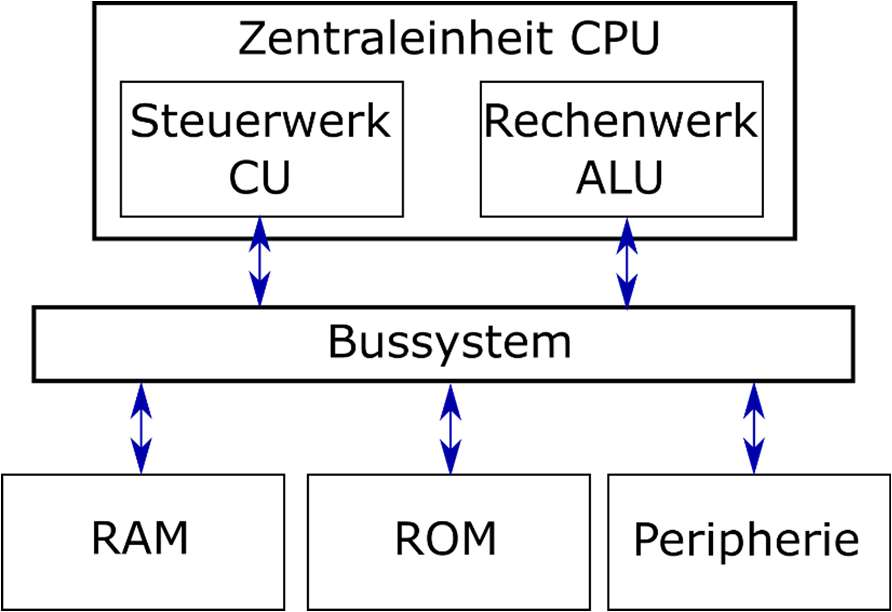
\includegraphics[width=3.125in,height=\textheight]{img/Kampl/AufbauES.jpg}
\caption{Aufbau eines Mikrocontrollers}
\end{figure}

\hypertarget{cpu}{%
\subparagraph{CPU}\label{cpu}}

Die CPU (Central Processing Unit) ist die primäre Steuereinheit eines
Systems. Sie besteht aus der ALU und der CU. Die ALU (Arithmetic Logic
Unit) ist der Teil der CPU, der arithmetisch-logische Operationen mit
binären Daten ausführt. Die CU (Control Unit) steuert mithilfe des
internen Oszillators die Abläufe im System. Nachdem ein Befehl decodiert
wurde, gibt die CU selbst weitere Befehle aus, um die korrekten Aktionen
zu starten. Diese Befehle werden dann über den Bus aus dem
Arbeitsspeicher abgerufen.

\hypertarget{bus}{%
\subparagraph{Bus}\label{bus}}

Der Bus verbindet die CPU mit den anderen Komponenten. Es gibt daher
verschiedene Arten von Bussen, wie z. B. den Datenbus, den Adressbus und
den Steuerbus. Je nach Prozessor können unterschiedlich viele Bits
gleichzeitig übertragen werden.

Des weiteren kann mann Busse noch in 2 Typen nach der Breite aufteilen:

\begin{enumerate}
\def\labelenumi{\arabic{enumi}.}
\tightlist
\item
  Parallel: Beim parallelen System gibt es mehrere Leitungen welche
  gleichzeitig Daten verschicken wodurch die Busbreite viel höher ist.
\item
  Seriell: Serielle Systeme übertragen Daten bitweise über eine einzelne
  Leitung, also nacheinander. Ein serieller Bus kann
  synchron,taktsignalbasiert, oder asynchron, durch Steuerleitungen und
  Protokolle koordiniert, arbeiten. Während ältere serielle Busse oft
  langsamer als parallele waren, sind moderne serielle Bussysteme durch
  höhere Taktraten und verbesserte Protokolle meist leistungsfähiger und
  effizienter.
\end{enumerate}

\hypertarget{schnittstellen}{%
\subparagraph{Schnittstellen}\label{schnittstellen}}

\begin{itemize}
\item
  \textbf{SPI:}\footnote{Serial Peripheral Interface} Eine synchrone
  serielle Schnittstelle, ideal für die Verbindung von Peripherigeräten.

  Es besteht aus den drei Leitungen POCI\footnote{Peripheral
    Out/Controller In} oder auch MISO\footnote{Master In/Slave Out},
  PICO/MOSI\footnote{Peripheral In/Controller Out \textbar{} Master
    Out/Slave In} und der Serial Clock. Außerdem dem gibt es noch den
  Slave-Select, aber da dies ein äußerst problematischer Außdruck ist
  wurde es zu Chip-Select umbenannt. Die Chip-Select Leitung sorgt
  dafür, dass der Controller ein Peripherigerät zur Kommuniaktion
  auswählt.

  Bei der SPI-Kommunikation gibt es keinen klaren Sender oder Empfänger,
  sondern einen kontinuierlichen Austausch, da sowohl die Peripherie als
  auch der Controller gleichzeitig ein Bit übertragen. Die Peripherie
  steuert die Kommunikation, indem sie die SCK-Impulse generiert,
  während der Controller das Signal annimmt und verarbeitet. Selbst wenn
  noch kein Ergebnis vorliegt, misst die Peripherie die Polarität der
  PICO/MOSI-Leitung und bestimmt daraus das nächste Bit.

  \begin{figure}
  \centering
  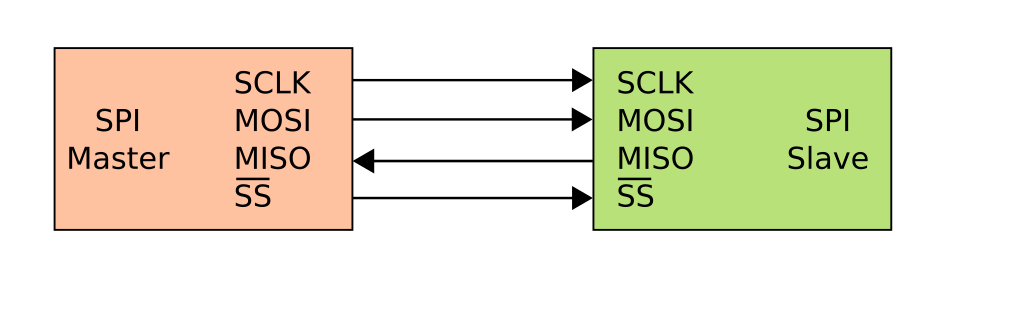
\includegraphics[width=4.16667in,height=\textheight]{img/Kampl/SPI-single-slave.svg.png}
  \caption{SPI-BUS-Grafik
  {[}\protect\hyperlink{ref-Serial-Peripheral-Interface-Grafik}{2}{]}}
  \end{figure}

  \begin{figure}
  \centering
  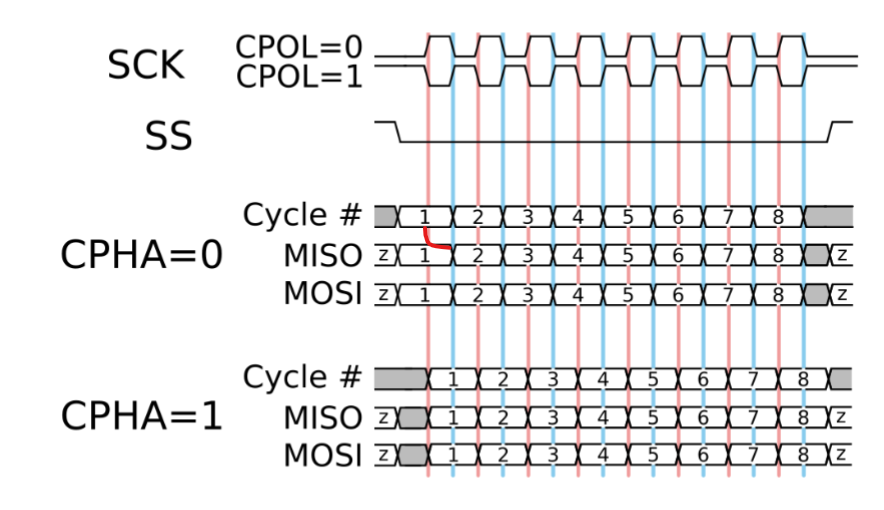
\includegraphics[width=4.16667in,height=\textheight]{img/Kampl/TimerDiagramm-SPI.png}
  \caption{SPI-Timerdiagramm
  {[}\protect\hyperlink{ref-Serielle-Schnittstellen}{3}{]}}
  \end{figure}
\item
  \textbf{UART:}\footnote{Universal Asynchronous Receiver Transmitter}
  Asynchrone serielle Verbindung, die ohne externen Taktgeber arbeitet.

  UART ist eine serielle Schnittstelle, die asynchron arbeitet. Sie
  wurde entwickelt, um die Kommunikation zwischen digitalen Geräten zu
  ermöglichen, und wird häufig in Mikrocontrollern, Computern und
  anderen elektronischen Geräten verwendet. Im Gegensatz zu synchronen
  Schnittstellen wie SPI oder I2C benötigt UART keine zusätzliche
  Taktleitung, sondern synchronisiert sich durch Start- und Stop-Bits.
  Der Datenaustausch erfolgt über zwei Leitungen, wobei ein Gerät als
  Sender und das andere als Empfänger fungiert.

  UART verwendet in der Regel zwei Hauptleitungen: TX\footnote{Transmit}
  zum Senden und RX\footnote{Receive} zum Empfangen von Daten.
  Zusätzlich können für die Hardware-Flow-Control weitere Leitungen
  genutzt werden, wie RTS\footnote{Request to Send}, mit dem der Sender
  signalisiert, dass er bereit ist, Daten zu übertragen, und
  CTS\footnote{Clear to Send}, das dem Sender anzeigt, dass der
  Empfänger bereit ist.

  \begin{figure}
  \centering
  \includegraphics[width=4.16667in,height=\textheight]{img/Kampl/I2C-Grafik.gif}
  \caption{I2C-BUS-Grafik
  {[}\protect\hyperlink{ref-I2C-Bus-Grafik}{4}{]}}
  \end{figure}

  \begin{figure}
  \centering
  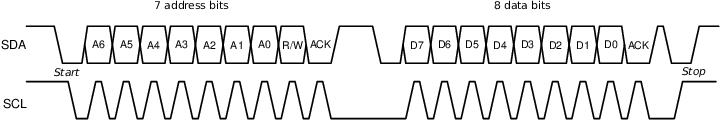
\includegraphics[width=4.16667in,height=\textheight]{img/Kampl/I2C-TimerDiagramm.png}
  \caption{I2C-Timerdiagramm
  {[}\protect\hyperlink{ref-I2C-TimerDiagramm}{5}{]}}
  \end{figure}
\item
  \textbf{I2C:}\footnote{Inter-Integrated Circuit} Serieller
  Zweidraht-Bus mit Master-Slave-Kommunikation.

  In einem I2C-Bus gibt es mindestens einen Master und bis zu 127
  Slaves. Ein Bus mit mehreren Mastern wird als Multi-Master-Bus
  bezeichnet. Jeder Slave benötigt eine eigene 7- oder 10-Bit-Adresse,
  um individuell mit einem Master kommunizieren zu können. Zusätzlich
  gibt es eine Broadcast-Adresse, über die alle Slaves gleichzeitig
  angesprochen werden können. Wie bei SPI beginnt die Kommunikation
  erst, wenn der Master einen Slave adressiert. Anders als bei SPI wird
  jedoch festgelegt, ob gesendet oder empfangen wird. Die Übertragung
  erfolgt durch Start- und Stopp-Bedingungen, die der Master über die
  Zustände der Takt- und Datenleitung steuert. Nach einer erfolgreichen
  Kommunikation senden die Slaves ihre Adresse und im Schreibfall ein
  Acknowledge.

  \begin{figure}
  \centering
  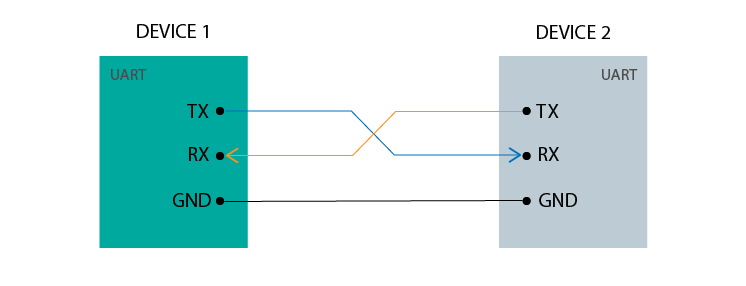
\includegraphics[width=4.16667in,height=\textheight]{img/Kampl/UART-Grafik.png}
  \caption{UART-Grafik {[}\protect\hyperlink{ref-UART-Grafik}{6}{]}}
  \end{figure}

  \begin{figure}
  \centering
  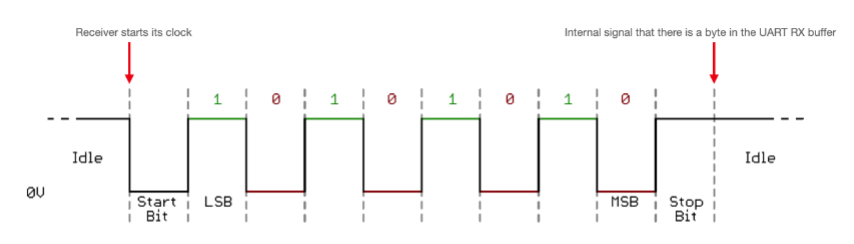
\includegraphics[width=4.16667in,height=\textheight]{img/Kampl/UART-TimerDiagramm.png}
  \caption{UART-Timerdiagramm
  {[}\protect\hyperlink{ref-Serielle-Schnittstellen}{3}{]}}
  \end{figure}
\end{itemize}

\hypertarget{ram}{%
\subparagraph{RAM}\label{ram}}

RAM ist eine Art Speichertyp, in welchem die Speicherzellen direkt
angesprochen werden. In diesem Zusammenhang spricht man dann von
\emph{Speicher mit wahlfreiem Zugriff}. Das heißt RAM erlaubt den
Zugriff jede Speicherzelle. RAM wird als Arbeitsspeicher verwendet, weil
es eine schnelle Verarbeitung vom Prozessor garantiert. Im Grunde
unterscheidet man zwischen zwei Arten von RAMs:

\begin{itemize}
\tightlist
\item
  \textbf{SRAM:}\footnote{Static RAM} Der schnellere der zwei Ram-Typen.
  Er speichert seine Inahlte mittels Flip-Flops und benötigt deshalb
  auch keine Refreshes. Jedoch ist der Einsatz von Flip-Flops äußerst
  Stromaufwendig und zu dem auch noch teuer. Trotzdem wird aufgrund eben
  dieser Kippglieder der SRAM häufig als Cache oder Puffer eingesetzt,
  da der Inhalt nach dem Abruf immer noch erhalten bleibt.
\item
  \textbf{DRAM:}\footnote{Dynamic RAM} Die einfache und billigere
  Variante. Der DRAM benutzt Kondensatoren als Speicherelement. Dabei
  muss über sogenannte Refreshes immer wieder die Spannung neugeladen
  werden wodurch der komplette Prozess langsamer wird. Jedoch hat er
  ingegensatz zum SRAM einen geringeren Stromverbrauch.
\end{itemize}

\hypertarget{rom}{%
\subparagraph{ROM}\label{rom}}

Wie der RAM ist auch der ROM eine Art Speicher. ROM-Speicher holt sich
den Befehlscode direkt aus den Programmspeicher. Der große Unterschied
zu anderen Speicherarten ist das der ROM, meist, nur lesenden Zugriff
erlaubt und nicht löschbar ist, daher auch der Name \textbf{Read Only
Memory}.

\begin{itemize}
\item
  \textbf{PROM}:\footnote{Programmable Read-Only Memory} Dieser
  Speichertyp kann nur einmal beschrieben werden. Beim Programmieren
  werden selektiv Sicherungen durchgebrannt, sodass die gespeicherten
  Daten nicht mehr verändert werden können.
\item
  \textbf{EPROM}:\footnote{Erasable Programmable Read-Only Memory}
  Dieser Speicher kann mit UV-Licht gelöscht werden. Dazu ist ein
  spezielles Quarzfenster erforderlich, durch das das UV-Licht die
  Speicherzellen erreicht und löscht, sodass der Speicher erneut
  beschrieben werden kann.
\end{itemize}

\begin{figure}
\centering
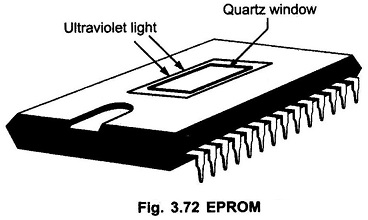
\includegraphics[width=3.125in,height=\textheight]{img/Kampl/EPROM.jpg}
\caption{EPROM {[}\protect\hyperlink{ref-EPROM}{7}{]}}
\end{figure}

\begin{itemize}
\item
  \textbf{OTP-EPROM}:\footnote{One-Time Programmable EPROM} Eine
  spezielle Variante des EPROM, die nicht mit UV-Licht gelöscht werden
  kann. Das liegt daran, dass der Speicher in ein lichtundurchlässiges
  Gehäuse eingeschweißt ist, wodurch ein erneutes Löschen verhindert
  wird.
\item
  \textbf{Flash}: Elektronisch lösch- und beschreibbarer Speicher, der
  in Blöcken oder einzelnen Sektoren selektiv gelöscht werden kann.
  Während das Schreiben und Löschen relativ langsam ist, erfolgt das
  Lesen sehr schnell. Flash-Speicher ersetzt zunehmend traditionelle
  ROM-Typen.
\end{itemize}

\begin{figure}
\centering
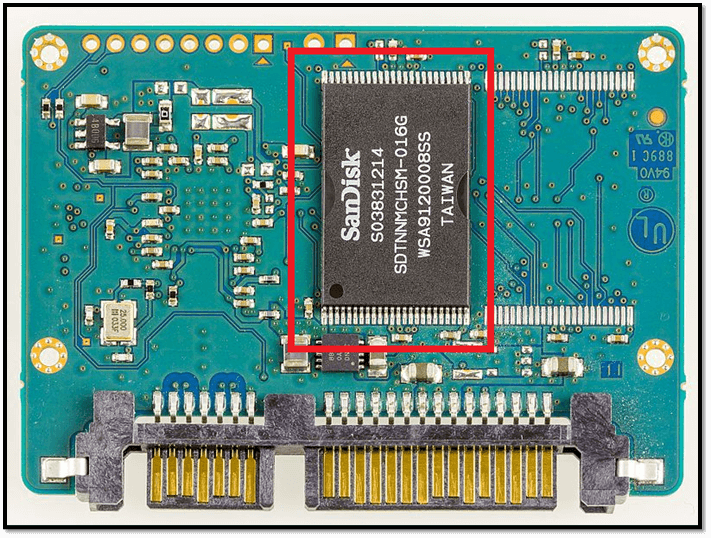
\includegraphics[width=3.125in,height=\textheight]{img/Kampl/Flash.png}
\caption{FLASH {[}\protect\hyperlink{ref-FLASH}{8}{]}}
\end{figure}

\begin{itemize}
\tightlist
\item
  \textbf{EEPROM}:\footnote{Electrically Erasable Programmable Read-Only
    Memory} Dieser Speicher kann elektrisch gelöscht und erneut
  beschrieben werden. Er wird oft für kleine, nichtflüchtige
  Datenspeicher wie Seriennummern oder MAC-Adressen in elektrischen
  Geräten verwendet. EEPROMs benötigen im Vergleich zu Flash-Speichern
  weniger Pins und werden meist seriell beschrieben.\\
  {[}\protect\hyperlink{ref-EmbeddedSystems}{1}{]}
\end{itemize}

\hypertarget{register}{%
\subparagraph{Register}\label{register}}

Register sind temporäre Speicher, die teils festgelegte
Verwendungszwecke (z. B. Befehls- oder Statusregister) haben und teils
für allgemeine Aufgaben genutzt werden.

\hypertarget{peripherie}{%
\subparagraph{Peripherie}\label{peripherie}}

\begin{itemize}
\item
  \textbf{GPIO}:\footnote{General Purpose Input/Output} GPIO-Pins sind
  flexibel nutzbare Ein- und Ausgänge eines Mikrocontrollers. Sie können
  als digitale Eingänge zur Erfassung von Tasterzuständen oder
  Sensordaten sowie als digitale Ausgänge zur Steuerung von LEDs,
  Motoren oder anderen Komponenten genutzt werden. Manche GPIOs verfügen
  über zusätzliche Funktionen, wie ADC-Eingänge oder Timer-Steuerung.
\item
  \textbf{Timer:} Das Timer-Modul dient zur Überwachung und Steuerung
  zeitkritischer Prozesse. Es kann als einfacher Zähler, zur Erzeugung
  von PWM-Signalen oder zur Zeitmessung verwendet werden.
  Timer-Interrupts ermöglichen präzise Steuerungen in
  Echtzeitanwendungen.
\item
  \textbf{Watchdog:} Der Watchdog-Timer erhöht die Sicherheit eines
  Systems, indem er einen automatischen Neustart auslöst, wenn das
  System nicht in regelmäßigen Abständen auf ihn reagiert. Dies
  verhindert ein Hängenbleiben oder Blockieren der Software und sorgt
  für eine höhere Zuverlässigkeit in Embedded-Systemen.
  Umgangssprachlich wird er als Totmansschalter bezeichnet.
\item
  \textbf{DMA}:\footnote{Direct Memory Access} Der Direct Memory Access
  ermöglicht es Peripheriegeräten, Daten direkt mit dem Speicher
  auszutauschen, ohne die CPU zu belasten. Dies beschleunigt den
  Datentransfer erheblich, insbesondere bei großen Datenmengen wie
  Audio- oder Videodaten, und verbessert die Gesamtleistung des
  Systems.\\
  {[}\protect\hyperlink{ref-EmbeddedSystems}{1}{]}
\end{itemize}

\hypertarget{firmware}{%
\subparagraph{Firmware}\label{firmware}}

Die Firmware ist eine softwarebasierte Komponente, die fest in einem
elektronischen Gerät implementiert ist und auf einem nicht-flüchtigen
Speicher abgelegt wird (z. B. Flash oder EEPROM). Sie verbindet Hardware
mit der Anwendungssoftware.

\hypertarget{recheneinheit}{%
\subparagraph{Recheneinheit}\label{recheneinheit}}

\begin{itemize}
\item
  \textbf{General-Purpose-Prozessoren:} Vielseitig einsetzbar und mit
  hoher Rechengeschwindigkeit ausgestattet. Sie verfügen über
  mehrschichtige Caches und sind für allgemeine Anwendungen optimiert,
  weisen jedoch keine integrierte Peripherie (wie Timer oder
  umfangreichen Speicher) auf, was sie weniger spezialisiert macht.
\item
  \textbf{Mikrocontroller:} In einem einzigen Chip vereint ein
  Mikrocontroller CPU, Speicher und Peripherieelemente (wie Bus-Treiber,
  PWM-Units, A/D- und D/A-Wandler). Diese enge Integration ermöglicht
  eine optimale Anpassung an spezifische Aufgaben in Embedded Systems,
  oft sogar ohne die Notwendigkeit eines externen Taktgebers, da interne
  Taktgeneratoren zur Verfügung stehen.
\item
  \textbf{Digitale Signalprozessoren (DSPs)}:\footnote{Digitale
    Signalprozessoren} Optimiert für die Echtzeit-Signalverarbeitung,
  bieten DSPs einen erweiterten Befehlssatz und spezielle
  Hardwareeinheiten -- etwa Multiply-Accumulate-Einheiten (MAC) -- zur
  effizienten Durchführung rechenintensiver Operationen, was sie ideal
  für Audio-, Video- und Kommunikationsanwendungen macht.
\item
  \textbf{ASICs}:\footnote{Application Specific Integrated Circuits}
  Diese speziell für bestimmte Anwendungen entwickelten Chips sind
  hinsichtlich Geschwindigkeit, Energieeffizienz, Baugröße und
  Zuverlässigkeit hoch optimiert. Ihre unflexible Natur und die hohen
  Kosten bei Entwicklung und Fertigung in kleinen Stückzahlen machen sie
  vor allem für Massenfertigung wirtschaftlich.
\item
  \textbf{FPGAs}:\footnote{Field-Programmable Gate Arrays}
  Programmierbare Hardwarebausteine, die vor der Verwendung nicht auf
  ein konkretes Verhalten festgelegt sind. FPGAs lassen sich mehrfach
  rekonfigurieren, was sie besonders in der Entwicklung (z.\,B. als
  Testumgebung für ASICs) attraktiv macht -- wenngleich sie im Vergleich
  zu spezialisierten Mikrocontrollern oft teurer sind und bei gleicher
  Technologie eine etwas geringere Performance bieten.
  {[}\protect\hyperlink{ref-EmbeddedSystems}{1}{]}
\end{itemize}

\hypertarget{zusuxe4tzliche-module}{%
\paragraph{Zusätzliche Module}\label{zusuxe4tzliche-module}}

\begin{itemize}
\tightlist
\item
  \textbf{A/D- und D/A-Wandler:}\footnote{Analog/Digital \&
    Digital/Analog Wandler} Ermöglichen die Umwandlung zwischen analogen
  und digitalen Signalen. Wichtig für Sensoranwendungen.
\item
  \textbf{PWM:}\footnote{Pulsweitenmodulation} Steuerung von LEDs,
  Motoren oder anderen Aktoren durch variable Einschaltdauer eines
  Signals.
\end{itemize}

\hypertarget{sensoren}{%
\subsubsection{Sensoren}\label{sensoren}}

\hypertarget{temperatur---thermometer}{%
\paragraph{Temperatur - Thermometer}\label{temperatur---thermometer}}

\hypertarget{luftdruck---barometer}{%
\paragraph{Luftdruck - Barometer}\label{luftdruck---barometer}}

\hypertarget{luftfeuchtigkeit---hygrometer}{%
\paragraph{Luftfeuchtigkeit -
Hygrometer}\label{luftfeuchtigkeit---hygrometer}}

\hypertarget{beschleunigung---accelerometer}{%
\paragraph{Beschleunigung -
Accelerometer}\label{beschleunigung---accelerometer}}

\hypertarget{gps}{%
\paragraph{GPS}\label{gps}}

\hypertarget{prototyping-mit-dem-eps32}{%
\subsubsection{Prototyping mit dem
EPS32}\label{prototyping-mit-dem-eps32}}

\hypertarget{ide}{%
\paragraph{IDE}\label{ide}}

Um ein Programm erfolgreich auf dem ESP32 ausführen zu können, benötigt
man eine geeignete IDE\footnote{Integrated Development Environment}.
Aber was genau ist eine IDE?

\begin{quote}
Eine integrierte Entwicklungsumgebung (IDE) ist Software für eine
optimierte Anwendungsentwicklung, die gängige Entwicklertools in einer
zentralen grafischen Oberfläche vereint.
{[}\protect\hyperlink{ref-RedHatIDE}{9}{]}
\end{quote}

Jede IDE enthält in der Regel ähnliche Standardkomponenten, darunter
einen integrierten Code-Editor -- also einen Texteditor mit
Syntax-Highlighting und gegebenenfalls Autovervollständigung --, ein
Programm zum Bauen und Kompilieren des Codes sowie einen Debugger.
{[}\protect\hyperlink{ref-RedHatIDE}{9}{]}

\hypertarget{vorteile}{%
\subparagraph{Vorteile}\label{vorteile}}

\textbf{IDEs bieten viele Vorteile, die beim Schreiben von Code
unterstützen.}

Während intelligente Code-Vervollständigung und -Generierung eher als
\emph{Nice-to-have}-Features gelten, gibt es echte Zeitersparnisse.
Besonders das \textbf{Echtzeit-Parsen von Code} spart erheblich Zeit bei
der Fehlersuche. Zudem beinhalten IDEs häufig Funktionen, die speziell
auf eine Programmiersprache zugeschnitten sind.

Ein Beispiel dafür ist \textbf{IntelliJ}, eine von der Firma JetBrains
entwickelte IDE, die speziell für Java konzipiert wurde. Sie bietet
unter anderem folgende Funktionen:

\begin{itemize}
\tightlist
\item
  \textbf{Generierung ganzer POJO-Klassen} per Knopfdruck
\item
  \textbf{Herunterladen von JDKs}\footnote{Java Development Kit}
\item
  \textbf{Darstellung von Dokumentationen} als Kommentaren im Fließtext
\end{itemize}

\hypertarget{platformio}{%
\paragraph{PlatformIO}\label{platformio}}

Eine der bekanntesten und am weitesten verbreiteten
Entwicklungsumgebungen für Mikrocontroller ist die Arduino IDE.
Allerdings stießen wir bei unserem Projekt auf Anforderungen, die mehr
Kontrolle über den Entwicklungs- und Upload-Prozess erforderten. Daher
entschieden wir uns für eine professionellere und flexiblere Lösung:
PlatformIO.

\begin{figure}
\centering
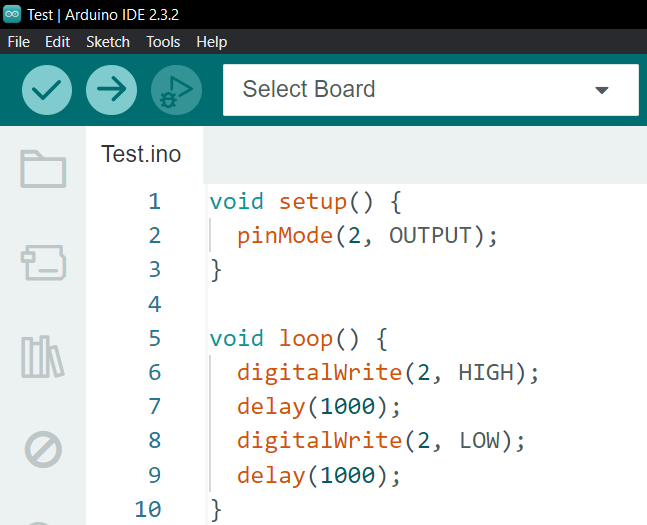
\includegraphics[width=4.16667in,height=\textheight]{img/Kampl/ArduinoIDE.png}
\caption{ArduinoIDE}
\end{figure}

\begin{center}\rule{0.5\linewidth}{0.5pt}\end{center}

\begin{figure}
\centering
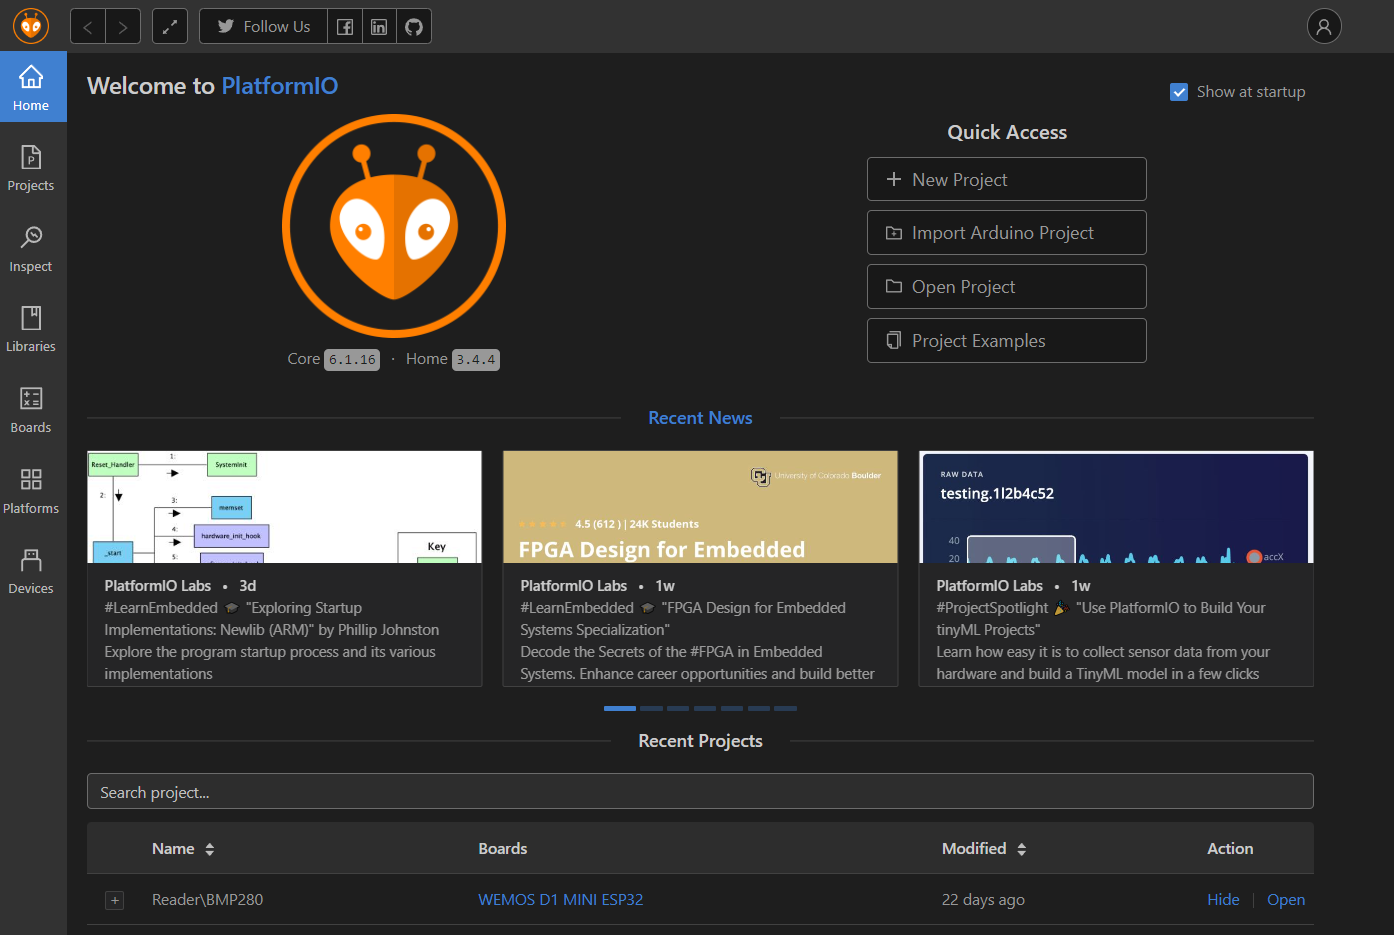
\includegraphics[width=5.20833in,height=\textheight]{img/Kampl/PlatformIO.png}
\caption{PlatformIO}
\end{figure}

PlatformIO ist eine Entwicklungsumgebung, die als Erweiterung für den
Texteditor Visual Studio Code genutzt wird. Sie bietet eine bessere
Projektstruktur, eine fortschrittlichere Konfigurationsverwaltung und
umfangreiche Unterstützung für verschiedene Mikrocontroller. Zwei
zentrale Elemente sorgen dabei für einen reibungslosen Ablauf: die
Hauptdatei (Main-File) und die Plattform-Konfigurationsdatei
(.ini-File). Besonders die .ini-Datei spielt eine entscheidende Rolle,
da sie die Projektkonfiguration festlegt und sicherstellt, dass der
Upload-Prozess auf den Mikrocontroller zuverlässig und ohne
Komplikationen funktioniert.

\begin{lstlisting}[caption={Beispiel einer .ini Datei für ein PlatformIO Projekt}]
    ; PlatformIO Project Configuration File
    ;
    ;   Build options: build flags, source filter
    ;   Upload options: custom upload port, speed and extra flags
    ;   Library options: dependencies, extra library storages
    ;   Advanced options: extra scripting
    ;
    ; Please visit documentation for the other options and examples
    ; https://docs.platformio.org/page/projectconf.html

    [env:board_name]
    platform = platform_name
    board = board_name
    framework = framework_name

    ; Zusätzliche Konfigurationsoptionen
    monitor_speed = 115200   ; Serielle Monitor-Geschwindigkeit
    upload_speed = 115200    ; Upload-Geschwindigkeit
    build_flags = -DDEBUG    ; Build-Flags hinzufügen
    lib_deps =               ; Bibliotheken hinzufügen
        library1
        library2
\end{lstlisting}

{[}\protect\hyperlink{ref-gpt-inifile}{10}{]}

\hypertarget{aufsetzen}{%
\subparagraph{Aufsetzen}\label{aufsetzen}}

Um PlatformIO benutzen zu können muss man die \emph{PlatformIO IDE} in
Visual Studio installieren. Nach der Installation und einem Neustart
kann man ein erstes Projekt erstellen.

Um nun ein erstes Projekt zu erstellen muss mann einfach nur auf den
PlatformIO Home Knopf drücken. Danach drückt man auf \emph{New Project}
und wähl das passende Board aus.
{[}\protect\hyperlink{ref-PlatformIO-firststeps}{11}{]}

\hypertarget{tools}{%
\subparagraph{Tools}\label{tools}}

\begin{figure}
\centering

\includegraphics[width=5.20833in,height=\textheight]{img/Kampl/platformio-ide-vscode-toolbar.png}
\caption{Toolbar von PlatformIO
{[}\protect\hyperlink{ref-PlatformIO-firststeps}{11}{]}}
\end{figure}

\begin{enumerate}
\def\labelenumi{\arabic{enumi}.}
\tightlist
\item
  \textbf{Home}: sorgt dafür, dass das Home Menü von PlatformIO. In
  diesem kann man seine Projekte verwalten sowie Bibiliothekten für das
  aktuelle hinzufügen.
\item
  \textbf{Build}: Kompiliert den Code des Projekts und erstellt eine
  Datei welche auf den Mikrocontroller hochgeladen werden kann.
\item
  \textbf{Upload}: Lädt die erstellte Datei von der Build Funktion auf
  das Festgelegte Zielgerät, in unseren Fall ein ESP32, hoch.

  \begin{enumerate}
  \def\labelenumii{\arabic{enumii}.}
  \tightlist
  \item
    Zuerst sucht PlatformIO nach richtigen Port. Entweder in der
    .ini-Datei festgelegt oder er wird automatisch erkannt.
  \item
    Die Firmware (.bin oder .hex Datei) wird auf das Gerät über den Port
    hochgeladen.
  \item
    Während des Uploads wird jeglicher Fortschritt im Terminal
    angezeigt.
  \end{enumerate}
\item
  \textbf{Clean}: Löscht alle temporären Dateien, welche beim
  Build-Prozess erstellt wurden. (z.B.: kompilierte Objektdateien, die
  Firmware-Datei). Im Grunde wird der /.pio Ordner gelöscht.
\item
  \textbf{Serial Port Monitor}: Öffnet eine Konsole innerhalb von Visual
  Studio, welche die Kommunikation zwischen dem ESP32 und dem Computer
  überwacht. Wichtig dabei ist zu beachten das die Baudrate richtig
  eingestellt ist. Übliche Baudraten sind 9600 sowie 115200. (Baud 8-N-1
  --\textgreater{} Ein Starbit, 8 Datenbits-Kein Paritätsbit-1 Stoppbit)
\item
  \textbf{Core (CLI)}: Ist eine Kommandozeilen-Toolbox, welche die
  vorher genannten Funktionen anbietet.
\item
  \textbf{Project Environment Switcher}: Erlaubt es zwischen
  verschiedenen Umgebungen innerhalb eines Projektes zu wechseln, falls
  sie vorhanden sind. Diese Umgebungen werden in der platformio.ini
  Datei angelegt. Das könnte ungefähr so aussehen:
\end{enumerate}

\begin{lstlisting}[caption={Beispiel Von Mehreren Umgebungen in PlatfromIO}]
[env:esp32]
platform = espressif32
board = esp32dev
framework = arduino

[env:stm32]
platform = ststm32
board = nucleo_f401re
framework = mbed
\end{lstlisting}

{[}\protect\hyperlink{ref-PlatformIO-firststeps}{11}{]}

\hypertarget{programmieren}{%
\subsubsection{Programmieren}\label{programmieren}}

Da wir nun eine vollständig funktionsfähige Entwicklungsumgebung
besitzen und auch wissen, wie man diese einsetzt, können wir mit der
tatsächlichen Programmierung starten. Wir verbinden den ESP32 mit
unserem Computer oder Laptop über ein USB-Kabel und schreiben unsere
ersten Code-Snippets, um zu testen, ob der Mikrocontroller ordnungsgemäß
funktioniert.

\begin{lstlisting}[language={C++}, caption={BME Testprogramm}]
// TestProgramm
void setup() {
  // Seriellen Monitor mit Baudrate 115200 starten
  Serial.begin(115200);
  Serial.println("ESP32 LED-Blinktest gestartet!");

  // LED-Setup (Standardmäßig GPIO 2 für die Onboard-LED)
  pinMode(LED_BUILTIN, OUTPUT);
}

void loop() {
  // LED ein
  Serial.println("LED AN");
  digitalWrite(LED_BUILTIN, HIGH);
  delay(500);

  // LED aus
  Serial.println("LED AUS");
  digitalWrite(LED_BUILTIN, LOW);
  delay(500);
}
\end{lstlisting}

Jetzt, da wir wissen, dass unser Gerät funktioniert, können wir mit der
weiteren Entwicklung beginnen. Zuerst sollten wir jeden einzelnen Sensor
separat ansprechen, um auch hier zu testen, ob die Sensoren
funktionieren. Ein Schritt nach dem anderen.

\hypertarget{bme280-als-temperatur-luftdruch-und-luftfeuchtigkeits-sensor}{%
\paragraph{BME280 als Temperatur, Luftdruch und Luftfeuchtigkeits
Sensor}\label{bme280-als-temperatur-luftdruch-und-luftfeuchtigkeits-sensor}}

Zuvor müssen wir jedoch einige Bibliotheken hinzufügen damit wir den
BME280 einfacher ansprechen können. Die verbreitetste Bibliothek ist die
\textbf{Adafruit BME280 Library}. Man fügt sie dem Projekt hinzu indem
man etweder man die folgende Zeile
\passthrough{\lstinline!adafruit/Adafruit BME280 Library@^2.2.4!} unter
dem Punkt \textbf{lib\_deps} in der .ini-Datei hinzufügt, oder indem man
PlatformIO verwendet, um die Library automatisch hinzuzufügen.

\begin{figure}
\centering
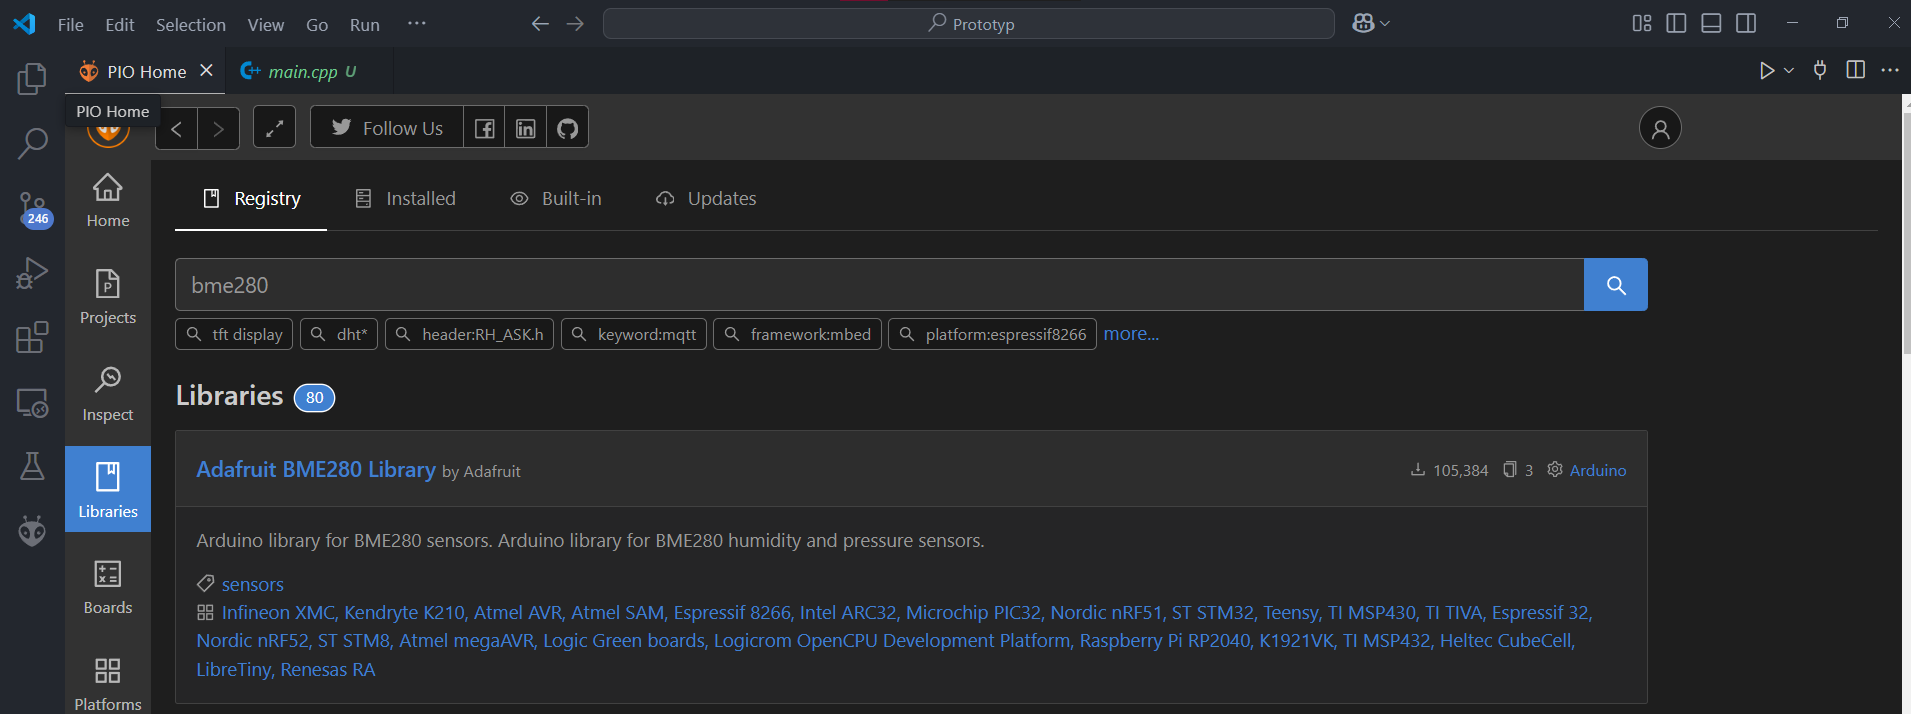
\includegraphics[width=5.20833in,height=\textheight]{img/Kampl/BME-Library.png}
\caption{BME-Library}
\end{figure}

Außerdem benötigt man noch die
\passthrough{\lstinline!adafruit/Adafruit BME280 Library@^2.2.4!},
welche als Schnittstelle für die Sensoren dient.

Am Ende verwenden wir folgenden Code für unseren Sensor:

\begin{lstlisting}[language={C++}, caption={BME Testprogramm}]
#include <Wire.h>
#include <Adafruit_Sensor.h>
#include <Adafruit_BME280.h>

#define SEALEVELPRESSURE_HPA (1013.25)

Adafruit_BME280 bme; 

unsigned long delayTime;

void printValues();

void setup() {
    Serial.begin(115200);
    Serial.println(F("BME280 test"));

    
    if (!bme.begin(0x76)) {
        Serial.println("Could not find a valid BME280 sensor, check wiring, address, sensor ID!");
        Serial.print("SensorID was: 0x"); Serial.println(bme.sensorID(),16);
        Serial.print("        ID of 0xFF probably means a bad address, a BMP 180 or BMP 085\n");
        Serial.print("   ID of 0x56-0x58 represents a BMP 280,\n");
        Serial.print("        ID of 0x60 represents a BME 280.\n");
        Serial.print("        ID of 0x61 represents a BME 680.\n");
        while (1) delay(10);
    }
    
    Serial.println("-- Default Test --");
    delayTime = 1000;

    Serial.println();
}


void loop() { 
    printValues();
    delay(delayTime);
}


void printValues() {
    Serial.print("Temperature = ");
    Serial.print(bme.readTemperature());
    Serial.println(" C");

    Serial.print("Pressure = ");

    Serial.print(bme.readPressure() / 100.0F);
    Serial.println(" hPa");

    Serial.print("Approx. Altitude = ");
    Serial.print(bme.readAltitude(SEALEVELPRESSURE_HPA));
    Serial.println(" m");

    Serial.print("Humidity = ");
    Serial.print(bme.readHumidity());
    Serial.println(" %");

    Serial.println();
}
\end{lstlisting}

{[}\protect\hyperlink{ref-BME280-Test}{12}{]}

\hypertarget{erkluxe4rung}{%
\subparagraph{Erklärung}\label{erkluxe4rung}}

Dieses Programm liest die Daten welche der BME280 Sensor bekommt aus der
I2C Schnittstelle aus und bereit sie über Print-Statements schnön
leserlich auf.

\textbf{\emph{Bibliotheken}}

\begin{lstlisting}[language={C++}, caption={Dependencies BME}]
#include <Wire.h>
#include <Adafruit_Sensor.h>
#include <Adafruit_BME280.h>
\end{lstlisting}

{[}\protect\hyperlink{ref-BME280-Test}{12}{]}

Dieser Teil zeigt die bereits vorhin Beschriebenen Bibliotheken mit
einer zusätzlichen der \textbf{Wire-Library}. Dies ist eine
Standardmäßige enthaltene Bibliothek und ermöglicht erst die I2C
Kommunikation.

\textbf{\emph{Definitionen und Variablen}}

\begin{lstlisting}[language={C++}, caption={Definition und Variablen BME}]
#define SEALEVELPRESSURE_HPA (1013.25)

Adafruit_BME280 bme; 

unsigned long delayTime;

void printValues();
\end{lstlisting}

{[}\protect\hyperlink{ref-BME280-Test}{12}{]}

\begin{enumerate}
\def\labelenumi{\arabic{enumi}.}
\tightlist
\item
  \textbf{SEALEVELPRESSURE\_HPA}: Ist eine Konstante welche den
  Standardluftdruck auf Meereshöhe annimmt.
\item
  \textbf{bme}: ist ein Instanz des Objektes Adafruit\_BME280 und stellt
  den Sensor dar.
\item
  \textbf{delayTime}: Ist eine Varible welche für einen delay verwendet
  wird.
\item
  \textbf{void printValues()}: Ist eine Vorwärtsdeklarierte Funktion.
\end{enumerate}

\textbf{\emph{Setup}}

\begin{lstlisting}[language={C++}, caption={Setup BME}]
void setup() {
    Serial.begin(115200);
    Serial.println(F("BME280 test"));

    
    if (!bme.begin(0x76)) {
        Serial.println("Could not find a valid BME280 sensor, check wiring, address, sensor ID!");
        Serial.print("SensorID was: 0x"); Serial.println(bme.sensorID(),16);
        Serial.print("        ID of 0xFF probably means a bad address, a BMP 180 or BMP 085\n");
        Serial.print("   ID of 0x56-0x58 represents a BMP 280,\n");
        Serial.print("        ID of 0x60 represents a BME 280.\n");
        Serial.print("        ID of 0x61 represents a BME 680.\n");
        while (1) delay(10);
    }
    
    Serial.println("-- Default Test --");
    delayTime = 1000;

    Serial.println();
}
\end{lstlisting}

{[}\protect\hyperlink{ref-BME280-Test}{12}{]}

Das Setup ist im Grunde der wichtigste Teil, da es alle wichtigen
Variablen, Modi usw. intialisiert. Es selbst ist hier in drei Teile
eingeteilt:

\begin{enumerate}
\def\labelenumi{\arabic{enumi}.}
\tightlist
\item
  \textbf{Serial.begin(115200)}: Hier wird die auf 115200 gestellt damit
  der serielle Monitor und der Sensor kommunizieren können.
\item
  \textbf{if(!bme.begin(0x76))}: Hier wird der Sensor mit der Adresse
  0x76 , wie im Datenblatt beschrieben, initialisiert.
  {[}\protect\hyperlink{ref-BME280-Datasheet}{13}{]}
\item
  \textbf{Fehlerbehandlung}: Falls der BME280 nicht gefunden wird oder
  nicht initialisiert werden kann kommt es zur Fehlerbehandlung und wenn
  nicht dann geht es weiter in den
\end{enumerate}

\textbf{\emph{Loop}}

\begin{lstlisting}[language={C++}, caption={Loop Funktion des BME Programms}]
void loop() { 
    printValues();
    delay(delayTime);
}
\end{lstlisting}

{[}\protect\hyperlink{ref-BME280-Test}{12}{]}

Wie der Name schon verrät wird der Loop immer wieder ausgeführt. In
diesem Fall hat der Loop die Funktionen
\passthrough{\lstinline!printValues()!} welche nach jedem Durchlauf
aufgerufen wird und \passthrough{\lstinline!delay()!}, mit der vorher
erwähnten \passthrough{\lstinline!delayTime!}, welche nach jedem Loop
eine Pause von einer Sekunde einlegt.

\textbf{\emph{Ausgabe}}

\begin{lstlisting}[language={C++}, caption={Ausgabe BME}]
void printValues() {
    Serial.print("Temperature = ");
    Serial.print(bme.readTemperature());
    Serial.println(" C");

    Serial.print("Pressure = ");
    Serial.print(bme.readPressure() / 100.0F);
    Serial.println(" hPa");

    Serial.print("Approx. Altitude = ");
    Serial.print(bme.readAltitude(SEALEVELPRESSURE_HPA));
    Serial.println(" m");

    Serial.print("Humidity = ");
    Serial.print(bme.readHumidity());
    Serial.println(" %");

    Serial.println();
}
\end{lstlisting}

{[}\protect\hyperlink{ref-BME280-Test}{12}{]}

Dieser Teil des Codes gibt die Messwerter auf dem Serial Monitor, in
einer aufpolierten Version aus. Der Grund für die Ausgabe ist meist
Debugging.

\begin{figure}
\centering
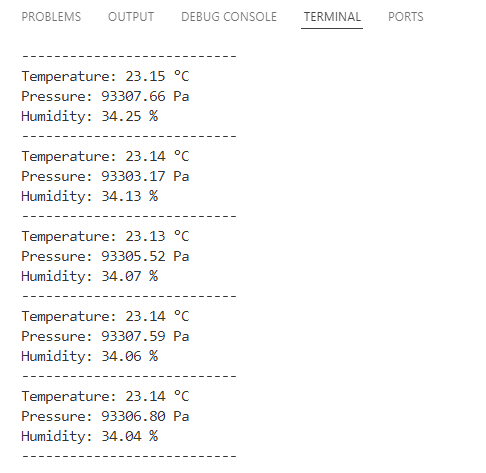
\includegraphics[width=5.20833in,height=\textheight]{img/Kampl/BME-Terminal.png}
\caption{BME-Ausgabe}
\end{figure}

\hypertarget{mpu6050-als-beschleunigungssensor}{%
\paragraph{MPU6050 als
Beschleunigungssensor}\label{mpu6050-als-beschleunigungssensor}}

Um nun auf diesen Sensor zugreifen zu können werden wieder einige
Bibliotheken benötigt welche man wieder in der Ini-Datei hinzufügen
muss. Über die Unified Sensor Library wurde schon geschrieben neu ist
die \passthrough{\lstinline!adafruit/Adafruit MPU6050 @ ^2.0.3!} Library
welche die verbindung zum Beschleunigungsensor vereinfacht.

Um nun tatsächlich Daten vom Sensor zu bekommen benutzt man folgendes
Programm

\begin{lstlisting}[language={C++}, caption={MPU Beispiel}]
// Basic demo for accelerometer readings from Adafruit MPU6050

#include <Adafruit_MPU6050.h>
#include <Adafruit_Sensor.h>
#include <Wire.h>

Adafruit_MPU6050 mpu;

void setup(void) {
  Serial.begin(115200);
  while (!Serial)
    delay(10); // will pause Zero, Leonardo, etc until serial console opens

  Serial.println("Adafruit MPU6050 test!");

  // Try to initialize!
  if (!mpu.begin()) {
    Serial.println("Failed to find MPU6050 chip");
    while (1) {
      delay(10);
    }
  }
  Serial.println("MPU6050 Found!");

  mpu.setAccelerometerRange(MPU6050_RANGE_8_G);
  Serial.print("Accelerometer range set to: ");
  switch (mpu.getAccelerometerRange()) {
  case MPU6050_RANGE_2_G:
    Serial.println("+-2G");
    break;
  case MPU6050_RANGE_4_G:
    Serial.println("+-4G");
    break;
  case MPU6050_RANGE_8_G:
    Serial.println("+-8G");
    break;
  case MPU6050_RANGE_16_G:
    Serial.println("+-16G");
    break;
  }
  mpu.setGyroRange(MPU6050_RANGE_500_DEG);
  Serial.print("Gyro range set to: ");
  switch (mpu.getGyroRange()) {
  case MPU6050_RANGE_250_DEG:
    Serial.println("+- 250 deg/s");
    break;
  case MPU6050_RANGE_500_DEG:
    Serial.println("+- 500 deg/s");
    break;
  case MPU6050_RANGE_1000_DEG:
    Serial.println("+- 1000 deg/s");
    break;
  case MPU6050_RANGE_2000_DEG:
    Serial.println("+- 2000 deg/s");
    break;
  }

  mpu.setFilterBandwidth(MPU6050_BAND_21_HZ);
  Serial.print("Filter bandwidth set to: ");
  switch (mpu.getFilterBandwidth()) {
  case MPU6050_BAND_260_HZ:
    Serial.println("260 Hz");
    break;
  case MPU6050_BAND_184_HZ:
    Serial.println("184 Hz");
    break;
  case MPU6050_BAND_94_HZ:
    Serial.println("94 Hz");
    break;
  case MPU6050_BAND_44_HZ:
    Serial.println("44 Hz");
    break;
  case MPU6050_BAND_21_HZ:
    Serial.println("21 Hz");
    break;
  case MPU6050_BAND_10_HZ:
    Serial.println("10 Hz");
    break;
  case MPU6050_BAND_5_HZ:
    Serial.println("5 Hz");
    break;
  }

  Serial.println("");
  delay(100);
}

void loop() {

  /* Get new sensor events with the readings */
  sensors_event_t a, g, temp;
  mpu.getEvent(&a, &g, &temp);

}
\end{lstlisting}

{[}\protect\hyperlink{ref-MPU6050-Test}{14}{]}

\hypertarget{erkluxe4rung-1}{%
\subparagraph{Erklärung}\label{erkluxe4rung-1}}

Dieses Programm liest die Daten welche der MPU6050 Sensor bekommt aus
der I2C Schnittstelle aus und bereit sie über Print-Statements schnön
leserlich auf.

\textbf{\emph{Bibliotheken}}

\begin{lstlisting}[language={C++}, caption={Dependencies MPU}]
#include <Wire.h>
#include <Adafruit_Sensor.h>
#include <Adafruit_MPU6050.h>
\end{lstlisting}

{[}\protect\hyperlink{ref-MPU6050-Test}{14}{]}

Dieser Teil zeigt die bereits beschreibt die schon beim BME
beschriebenen Bibliotheken + der MPU Bibliothek.

\textbf{\emph{Definitionen und Variablen}}

\begin{lstlisting}[language={C++}, caption={Definition und Variablen MPU}]
Adafruit_MPU6050 mpu;
\end{lstlisting}

\begin{enumerate}
\def\labelenumi{\arabic{enumi}.}
\setcounter{enumi}{1}
\tightlist
\item
  \textbf{mpu}: ist ein Instanz des Objektes Adafruit\_MPU6050 und
  stellt den Sensor dar.
\end{enumerate}

\textbf{\emph{Setup}}

\begin{lstlisting}[language={C++}, caption={Setup MPU}]
void setup(void) {
  Serial.begin(115200);
  while (!Serial)
    delay(10); // will pause Zero, Leonardo, etc until serial console opens

  Serial.println("Adafruit MPU6050 test!");

  // Try to initialize!
  if (!mpu.begin()) {
    Serial.println("Failed to find MPU6050 chip");
    while (1) {
      delay(10);
    }
  }
  Serial.println("MPU6050 Found!");

  mpu.setAccelerometerRange(MPU6050_RANGE_8_G);
  Serial.print("Accelerometer range set to: ");
  switch (mpu.getAccelerometerRange()) {
  case MPU6050_RANGE_2_G:
    Serial.println("+-2G");
    break;
  case MPU6050_RANGE_4_G:
    Serial.println("+-4G");
    break;
  case MPU6050_RANGE_8_G:
    Serial.println("+-8G");
    break;
  case MPU6050_RANGE_16_G:
    Serial.println("+-16G");
    break;
  }
  mpu.setGyroRange(MPU6050_RANGE_500_DEG);
  Serial.print("Gyro range set to: ");
  switch (mpu.getGyroRange()) {
  case MPU6050_RANGE_250_DEG:
    Serial.println("+- 250 deg/s");
    break;
  case MPU6050_RANGE_500_DEG:
    Serial.println("+- 500 deg/s");
    break;
  case MPU6050_RANGE_1000_DEG:
    Serial.println("+- 1000 deg/s");
    break;
  case MPU6050_RANGE_2000_DEG:
    Serial.println("+- 2000 deg/s");
    break;
  }

  mpu.setFilterBandwidth(MPU6050_BAND_21_HZ);
  Serial.print("Filter bandwidth set to: ");
  switch (mpu.getFilterBandwidth()) {
  case MPU6050_BAND_260_HZ:
    Serial.println("260 Hz");
    break;
  case MPU6050_BAND_184_HZ:
    Serial.println("184 Hz");
    break;
  case MPU6050_BAND_94_HZ:
    Serial.println("94 Hz");
    break;
  case MPU6050_BAND_44_HZ:
    Serial.println("44 Hz");
    break;
  case MPU6050_BAND_21_HZ:
    Serial.println("21 Hz");
    break;
  case MPU6050_BAND_10_HZ:
    Serial.println("10 Hz");
    break;
  case MPU6050_BAND_5_HZ:
    Serial.println("5 Hz");
    break;
  }

  Serial.println("");
  delay(100);
}
\end{lstlisting}

{[}\protect\hyperlink{ref-MPU6050-Test}{14}{]}

\begin{enumerate}
\def\labelenumi{\arabic{enumi}.}
\tightlist
\item
  \textbf{Serial.beginn(115200)}: Hier wird die auf 115200 gestellt
  damit der serielle Monitor und der Sensor kommunizieren können.
\item
  \textbf{if (!mpu.begin())}: Hier wird der Sensor initialisiert.
\item
  \textbf{mpu.setAccelerometerRange(MPU6050\_RANGE\_8\_G)}: Ist die
  Auflösung des Beschleunigungssensor, also in welchen Bereich, und wie
  genau, gemessen wird. Desto kleiner der G-Wert\footnote{Erdbeschleunigung}
  desto genauer die Auflösung und desto kleiner der Messbereich.
\end{enumerate}

\begin{longtable}[]{@{}ll@{}}
\toprule
G-Bereich & Max. Messwert\tabularnewline
\midrule
\endhead
±2G & 19,62 m/s²\tabularnewline
±4G & 39,24 m/s²\tabularnewline
±8G & 78,48 m/s²\tabularnewline
±16G & 156,96 m/s²\tabularnewline
\bottomrule
\end{longtable}

\begin{enumerate}
\def\labelenumi{\arabic{enumi}.}
\setcounter{enumi}{3}
\tightlist
\item
  \textbf{mpu.setGyroRange(MPU6050\_RANGE\_500\_DEG)}: Dieser Teil setzt
  den Messbereich des Gyroskops fest. Um genauer zu sein in diesen fall
  auf +-500 Grad/Sekunde. Auch hier gilt das Prinzip wieder, je größer
  der Bereich desto kleiner die Auflösung.
\end{enumerate}

\begin{longtable}[]{@{}ll@{}}
\toprule
Konstantenname & Messbereich\tabularnewline
\midrule
\endhead
\passthrough{\lstinline!MPU6050\_RANGE\_250\_DEG!} & ±250
°/s\tabularnewline
\passthrough{\lstinline!MPU6050\_RANGE\_500\_DEG!} & ±500 °/s
(gesetzt)\tabularnewline
\passthrough{\lstinline!MPU6050\_RANGE\_1000\_DEG!} & ±1000
°/s\tabularnewline
\passthrough{\lstinline!MPU6050\_RANGE\_2000\_DEG!} & ±2000
°/s\tabularnewline
\bottomrule
\end{longtable}

\begin{enumerate}
\def\labelenumi{\arabic{enumi}.}
\setcounter{enumi}{4}
\tightlist
\item
  \textbf{mpu.setFilterBandwidth(MPU6050\_BAND\_21\_HZ)}: Hier wird die
  Brandweite angepasst um einzustellen Welche werte der Sensor misst und
  welche er nur als Rauschen wahrnimmt.
\end{enumerate}

\textbf{\emph{Loop}}

\begin{lstlisting}[language={C++}, caption={Loop Funktion des MPU Sensors}]
void loop() { 
  sensors_event_t a, g, temp;
  mpu.getEvent(&a, &g, &temp);

  Serial.print("Acceleration X: ");
  Serial.print(a.acceleration.x);
  Serial.println(" m/s^2");
}
\end{lstlisting}

{[}\protect\hyperlink{ref-MPU6050-Test}{14}{]}

Der Loop ist eine grundlegende Struktur in Arduino-Sketches, die
kontinuierlich ausgeführt wird, solange das Programm läuft. Hier ist
eine detaillierte Erklärung der einzelnen Komponenten.
\textbf{sensors\_event\_t a, g, temp}: Diese Zeile deklariert drei
Variablen mit dem Typ sensors\_event\_t. Diese Variablen werden
verwendet, um die Ereignisdaten für die Beschleunigung (a), die
Drehgeschwindigkeit (g) und die Temperatur (temp) zu speichern.
\textbf{mpu.getEvent(\&a, \&g, \&temp);}: Diese Funktion ruft die
neuesten Sensordaten vom MPU6050-Sensor ab und speichert sie in den
Variablen von vorher.

Außerdem gibt der Loop wieder die Werte über Print-Statements aus um sie
auf dem Serial Monitor sehen zu können.

\begin{figure}
\centering
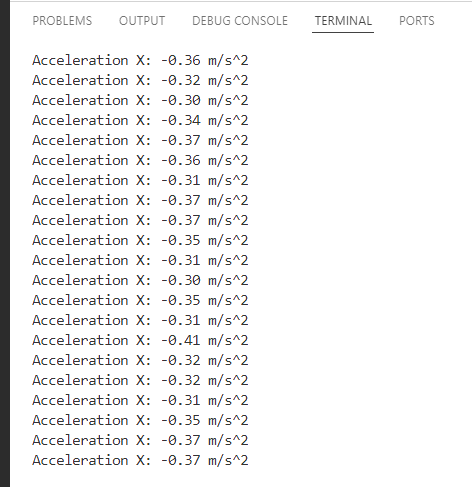
\includegraphics[width=5.20833in,height=\textheight]{img/Kampl/MPU-Terminal.png}
\caption{MPU-Ausgabe}
\end{figure}

\hypertarget{gy-gpsmv2-sensor-zur-bestimmung-der-postition-mittels-gps}{%
\paragraph{GY-GPSMV2 Sensor zur Bestimmung der Postition mittels
GPS}\label{gy-gpsmv2-sensor-zur-bestimmung-der-postition-mittels-gps}}

Der letzte Sensor zur Realisierung ist das GPS-Modul GY-GPSMV2. Im
Grunde werden für diesen Sensor keine weiteren Bibliotheken benötigt
jedoch kommt dazu gleich noch mehr. Um nun die GPS-Postion in seiner
NMEA\footnote{National Marine Electronics Association} Rohform auslesen
zu können, greift man mit dem folgenden Programm auf die
UART-Schnittstelle des Sensors zu.

\begin{lstlisting}[language={C++}, caption={GY-GPSMV2 Test Programm mit Daten in Rohform}]
#define RXD2 16
#define TXD2 17

#define GPS_BAUD 9600

// Create an instance of the HardwareSerial class for Serial 2
HardwareSerial gpsSerial(2);

void setup(){
  // Serial Monitor
  Serial.begin(115200);
  
  // Start Serial 2 with the defined RX and TX pins and a baud rate of 9600
  gpsSerial.begin(GPS_BAUD, SERIAL_8N1, RXD2, TXD2);
  Serial.println("Serial 2 started at 9600 baud rate");
}

void loop(){
  while (gpsSerial.available() > 0){
    // get the byte data from the GPS
    char gpsData = gpsSerial.read();
    Serial.print(gpsData);
  }
  delay(1000);
  Serial.println("-------------------------------");
}
\end{lstlisting}

{[}\protect\hyperlink{ref-GPS-Testprogramm}{15}{]}

\hypertarget{erkluxe4rung-2}{%
\subparagraph{Erklärung}\label{erkluxe4rung-2}}

\textbf{\emph{Variablen für das GPS-Modul}}

\begin{lstlisting}[language={C++}, caption={GY-GPSMV2 Variablen}]
  #define RXD2 16
  #define TXD2 17
  #define GPS_BAUD 9600

  HardwareSerial gpsSerial(2);
\end{lstlisting}

\begin{enumerate}
\def\labelenumi{\arabic{enumi}.}
\tightlist
\item
  \textbf{RXD2}: Ist eine Konstante, die den GPIO-Pin 16 für den Empfang
  von Daten definiert.\\
\item
  \textbf{TXD2}: Ist eine Konstante, die den GPIO-Pin 17 für das Senden
  (TX) von Daten definiert.\\
\item
  \textbf{GPS\_BAUD}: Ist eine Konstante, die die Baudrate von 9600, wie
  im Datenblatt angegeben, für die Kommunikation mit dem Sensor
  festlegt. {[}\protect\hyperlink{ref-GPS-Baudrate}{16}{]}
\item
  \textbf{gpsSerial(2)}: Hier wird eeine Instanz des HardwareSerial
  Objektes auf UART-Port2 erstellt um mit dem Mikrocontroller zu
  kommunizieren
\end{enumerate}

\textbf{\emph{Setup für das GPS-Modul}}

\begin{lstlisting}[language={C++}, caption={GY-GPSMV2 Setup}]
void setup(){
  // Serial Monitor
  Serial.begin(115200);
  
  // Start Serial 2 with the defined RX and TX pins and a baud rate of 9600
  gpsSerial.begin(GPS_BAUD, SERIAL_8N1, RXD2, TXD2);
  Serial.println("Serial 2 started at 9600 baud rate");
}
\end{lstlisting}

Wie auch schon bei den anderen Sensoren muss auch hier zuerst eine
Baudrate, in diesen Fall 115200, für die Kommunikation initialisiert
werden. Mithilfe von \passthrough{\lstinline!gpsSerial!} wird eine
Serielle Verbindung zum GPS-Modul hersgestellt in welcher die Baudrate,
die Standard-Konfiguration von 8-Datenbits, keine Parität, der Stoppbit
und die zwei Schnittstellen übergeben werden. Desweiteren gibt es noch
das Print-Statement um den Fortschritt auf dem Serial Monitor sehen zu
können.

\textbf{\emph{Loop Funktionen für das GPS-Modul (NMEA)}}

\begin{lstlisting}[language={C++}, caption={GY-GPSMV2 Test Programm mit Daten in Rohform}]
void loop(){
  while (gpsSerial.available() > 0){
    // get the byte data from the GPS
    char gpsData = gpsSerial.read();
    Serial.print(gpsData);
  }
  delay(1000);
  Serial.println("-------------------------------");
}
\end{lstlisting}

Die Loop Funktion für das GPS-Modul überprüft zuerst, ob Daten momentan
verfügbar sind. Dies regelt sie mithilfe der While-Schleife:
\passthrough{\lstinline!while (gpsSerial.available() > 0)!}. Um nun die
NMEA-Daten zu Printen, werden sie zuerst in einem char-Datentypen
gespeichert und danach mittels
\passthrough{\lstinline!Serial-print(gpsData);!} auf dem Serial Monitor
ausgebene werden können.

\textbf{\emph{Loop Funktionen für das GPS-Modul (Aufbereitet)}}

Das Proplem mit NMEA Daten ist, das sie unleserlich sind

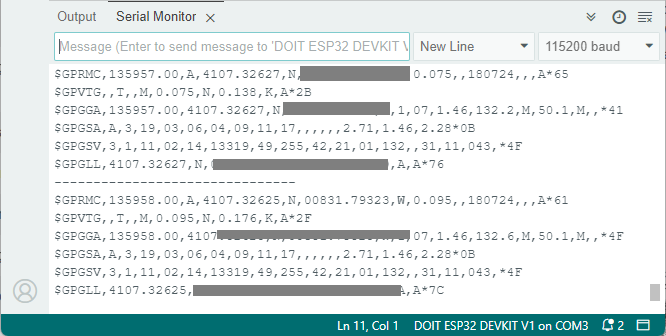
\includegraphics[width=5.20833in,height=\textheight]{img/Kampl/NMEA-Ausgabe.png}
{[}\protect\hyperlink{ref-GPS-Testprogramm}{15}{]}

Deshalb, benötigt man doch noch eine Bibliothek und zwar
\textbf{TinyGPSPlus}. Man fügt wie immer diese Bibliothek in der
Ini-Datei hinzu, diesesmal mit auf folgende Weise:
\passthrough{\lstinline!mikalhart/TinyGPSPlus@^1.1.0!}.

Danach wird der Code hierum erweitert:

\begin{lstlisting}[language={C++}, caption={GY-GPSMV2 Erweiterung mit verarbeiteten Daten}]
TinyGPSPlus gps;

void loop() {
  // This sketch displays information every time a new sentence is correctly encoded.
  unsigned long start = millis();

  while (millis() - start < 1000) {
    while (gpsSerial.available() > 0) {
      gps.encode(gpsSerial.read());
    }
    if (gps.location.isUpdated()) {
      Serial.print("LAT: ");
      Serial.println(gps.location.lat(), 6);
      Serial.print("LONG: "); 
      Serial.println(gps.location.lng(), 6);
      Serial.print("SPEED (km/h) = "); 
      Serial.println(gps.speed.kmph()); 
      Serial.print("ALT (min)= "); 
      Serial.println(gps.altitude.meters());
      Serial.print("HDOP = "); 
      Serial.println(gps.hdop.value() / 100.0); 
      Serial.print("Satellites = "); 
      Serial.println(gps.satellites.value()); 
      Serial.print("Time in UTC: ");
      Serial.println(String(gps.date.year()) + "/" + String(gps.date.month()) + "/" + String(gps.date.day()) + "," + String(gps.time.hour()) + ":" + String(gps.time.minute()) + ":" + String(gps.time.second()));
      Serial.println("");
    }
  }
}
\end{lstlisting}

Die TinyGPSPlus bietet viele Funktionen zur leserlichen Darstellung der
GPS-Daten. Die wichtigste von ihnen ist die
\passthrough{\lstinline!gps.encode()!} Funktionen welche die
unleserlichen NMEA dekodiert und verarbeitet. Danach wird mithilfe eines
IF-Statements darauf geachtet, ob sich die Position des Gerätes
verändert hat \passthrough{\lstinline!if(gps.locaton.isUpdated())!}. Und
zum Schluss gibt es alle möglichen Daten, wie den Längen und
Breitengrad, des Sensors aus.

\hypertarget{datenuxfcbertragung}{%
\subsubsection{Datenübertragung}\label{datenuxfcbertragung}}

\hypertarget{mqtt}{%
\paragraph{MQTT}\label{mqtt}}

\begin{quote}
MQTT (Message Queuing Telemetry Transport) ist ein Nachrichtenprotokoll
für eingeschränkte Netzwerke mit geringer Bandbreite und IoT-Geräte mit
extrem hoher Latenzzeit. Da Message Queuing Telemetry Transport auf
Umgebungen mit niedriger Bandbreite und hoher Latenz spezialisiert ist,
ist es ein ideales Protokoll für die Machine-to-Machine-Kommunikation
{[}\protect\hyperlink{ref-Inray-GmbH}{17}{]}
\end{quote}

MQTT wird häufig in IoT-Anwendungen\footnote{Internet of Things}
aufgrund eben dieser geringen benötigten Bandbreite verwendet, da es
dadurch sehr zuverlässig arbeitet und selbst bei schlechter
Netzwerkverbindung funktioniert.

Einige Wichtige Begriffe im Zusammenhang mit MQTT sind

\begin{itemize}
\tightlist
\item
  \textbf{Publisher}: Der Sender, der Informationen oder Daten an den
  Broker schickt.
\item
  \textbf{Subscriber}: Der Empfänger, der sich beim Broker anmeldet, um
  bestimmte Nachrichten zu erhalten.
\item
  \textbf{Broker}: Ist ein Vermittler, zum Beispiel ein Server, welcher
  Nachrichten von Publishern/Sendern entgegennimmt und sie and
  Subscribern/Empfängern weiterleitet.
\item
  \textbf{Topic}: Eine Art ``Kategorien'' in welchen Nachrichten
  veröffentlicht werden. Diese Kategorien können von von Empfänger
  abonniert werden um diese Nachrichten zu bekommen.
\end{itemize}

\hypertarget{wlan-mesh}{%
\subsubsection{WLAN-Mesh}\label{wlan-mesh}}

Ein Mesh ist ein System/Netzwerk, welches aus mehreren
WLAN-Zugangspunkten, songenannten Access Points, besteht. Es sorgt
dafür, dass diese Access Points eine lückenlose WLAN-Abdeckung
zugesichert werden kann.

Um nun ein Mesh-Netzwerk nun aufbauen zu können muss man zuerst die
einzelnen Knotenpunkte miteinander verbinden. Dabei ist immer mindestens
einer dieser Punkte mit einem Router oder Modem verbunden um eine
Verbindung mit dem Internet herzustellen. Die restlichen Knoten
kommunizieren dann drahtlos untereinander. {[}vgl.@EK-WlanMesh{]} Wenn
nun ein Knoten Daten sendet werden sie von nächstgelegenen Knoten auch
aufgenommen. Die Daten werden dann von Knoten zu Knoten weitergeleitet
bis sie den Hauptknoten erreichen und zum Schluss im Internet landen.
Dieser Prozess wird Hop-to-Hop Kommunikation
genannt.{[}vgl.@Wikipedia-Hop{]} Ein weiters wichtiges Merkmal eines
Meshes ist, das songenannte Seamless-Roaming. Dabei wechseln die
einzelnen Knoten immer zu Access Point mit dem stärksten Signal ohne,
dass die Verbindung unterbrochen wird. Des weiteren verfügt ein Mesh
über eine Selbstheilungsfunktion. D.h.: Wenn ein Knotenpunkt, aus
verschiedensten Gründen, ausfällt oder die Verbindung verliert, so sucht
das System automatisch nach einer alternativen Route über andere
Knotenpunkte um wieder eine stabile Verbindung
aufzubauen.{[}vgl.@EK-WlanMesh{]}

\hypertarget{sonstiges}{%
\subsubsection{Sonstiges}\label{sonstiges}}

\hypertarget{github-actions}{%
\paragraph{GitHub Actions}\label{github-actions}}

GitHub Actions ist ein Tool zur Automatisierung von Softwareprozessen
wie dem Testen und Bereitstellen von Code. Ein zentrales Feature ist
\textbf{CI/CD}\footnote{Continuous Integration und Continuous
  Delivery/Deployment}, das automatisch Code ändert und veröffentlicht.
Nach erfolgreichem Abschluss aller Tests kann der neue Code automatisch
ins Repository übertragen werden.

Actions haben noch viele weitere Funktionen da sie im Grunde eine
Virtuelle Umgebung erschaffen in welcher Code ausgeführt werden kann.

Um einen \textbf{Workflow} zu erstellen, legt man, im vorher erstellten
Woreine \textbf{YAML-Datei} an, die folgende Elemente definiert:

\begin{itemize}
\tightlist
\item
  \textbf{Event}: Der Auslöser des Workflows (z. B. ein neuer
  Code-Push).\\
\item
  \textbf{Jobs}: Die Aufgaben, die nach dem Event ausgeführt werden.\\
\item
  \textbf{Runner}: Die Umgebung, in der der Code läuft (z. B. Ubuntu,
  Windows, macOS).\\
\item
  \textbf{Steps \& Actions}: Schritte innerhalb eines Jobs, die
  bestimmte Aktionen ausführen, wie z. B. das Testen oder Überprüfen des
  Codes.
\end{itemize}

\newpage

\hypertarget{praktische-arbeit}{%
\subsection{Praktische Arbeit}\label{praktische-arbeit}}

\hypertarget{entwicklung-des-prototypen}{%
\subsubsection{Entwicklung des
Prototypen}\label{entwicklung-des-prototypen}}

\hypertarget{benuxf6tigte-hardwarekomponenten}{%
\paragraph{Benötigte
Hardwarekomponenten}\label{benuxf6tigte-hardwarekomponenten}}

Um ein Projekt zu realisieren, bei dem Umweltdaten ausgelesen werden,
benötigt man geeignete Komponenten, auf denen die Software zuverlässig
läuft. Bei der Auswahl dieser Komponenten spielten mehrere Faktoren eine
Rolle, darunter die Kosten, die Größe, die Anwendungsfälle sowie die
Anzahl der verfügbaren Funktionen. Des weiteren ist zu beachten, dass
die Diplomarbeit mehr ein \emph{Proof of Concept} sein soll.

Unser finaler Prototyp sollte folgende physikalischen Messwerte erfassen
können.

\begin{itemize}
\tightlist
\item
  Temperatur
\item
  Luftfeuchtigkeit
\item
  Luftdruck
\item
  Beschleunigung und Geschwindigkeit
\item
  Standortbestimmung mittels GPS

  \begin{itemize}
  \tightlist
  \item
    Breiten/- Längengrade
  \item
    Meereshöhe
  \end{itemize}
\end{itemize}

Nach sorgfältiger Abwägung haben wir uns schließlich für die folgenden
Komponenten entschieden:

\hypertarget{esp32}{%
\subparagraph{ESP32}\label{esp32}}

\textbf{Grund}: Der ESP32 ist ein leistungsstarker und kostengünstiger
Mikrocontroller mit integrierter WLAN- und Bluetooth Funktionalität. Er
bietet eine höhere Rechenleistung als ein Arduino und ist im
durchschnitt auch kleiner als jener, was für die mobile Nutzung vom
Vorteil ist. \textbf{Spezifikationen}:

\begin{lstlisting}
 - Größe: $39mm  *  28mm  *  6mm$
 - 34 I/O Pins
 - SoC: ESP32-WROOM-32
 - Netzspannung: 5V
\end{lstlisting}

\begin{figure}
\centering
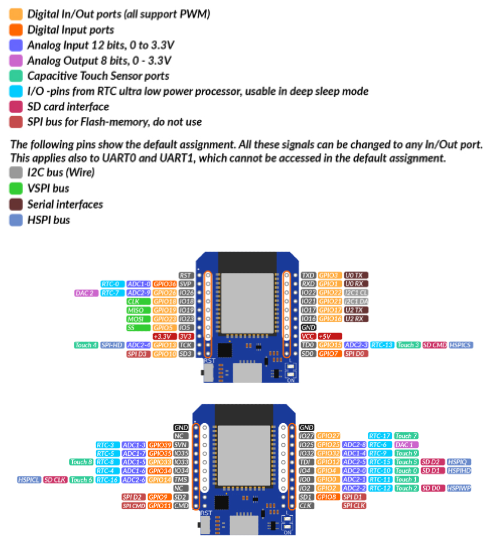
\includegraphics[width=5.20833in,height=\textheight]{img/Kampl/ESP32-Pins.png}
\caption{ESP32-Pins {[}\protect\hyperlink{ref-ESP32-Datenblatt}{18}{]}}
\end{figure}

\hypertarget{bme280}{%
\subparagraph{BME280}\label{bme280}}

\textbf{Grund}: Der BME280 ist ein vielseitiger Sensor, welcher sowohl
die Temperatur, die Luftfeuchtigkeit als auch den Luftdruck messen kann.
Außerdem ist er kompakt und kostengünstig. \textbf{Spezifikationen}:

\begin{lstlisting}
 - Größe: $9mm  *  11mm  *  2mm$
 - 4 Pins
 - Schnittstelle I2C
 - Spannung: 3.3V bis 5V
\end{lstlisting}

\begin{figure}
\centering
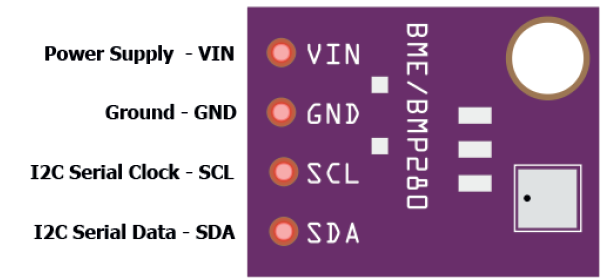
\includegraphics[width=3.125in,height=\textheight]{img/Kampl/BME280-Pins.png}
\caption{BMEPins {[}\protect\hyperlink{ref-BME280-Datenblatt}{19}{]}}
\end{figure}

\hypertarget{mpu6050}{%
\subparagraph{MPU6050}\label{mpu6050}}

\textbf{Grund}: Der MPU6050 ist eine Kombination aus
Beschleungiungssensor und Gyroskop. Damit können Bewegungen auf der X,
der Y und der Z-Achse erfasst werden. \textbf{Spezifikationen}:

\begin{lstlisting}
 - Größe: $25mm  *  20mm  *  7mm$
 - 8 Pins
 - Schnittstelle I2C
 - Spannung: 3.3V bis 5V
\end{lstlisting}

\begin{figure}
\centering
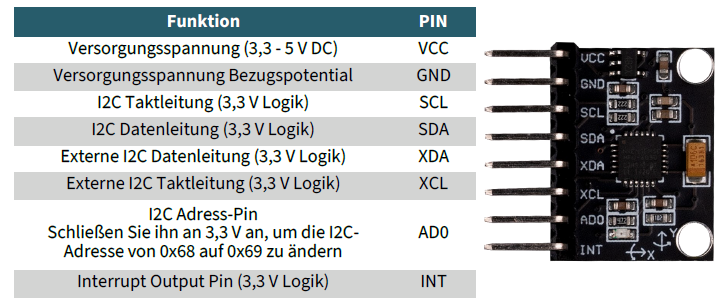
\includegraphics[width=5.20833in,height=\textheight]{img/Kampl/MPU6050-Pins.png}
\caption{MPUPins {[}\protect\hyperlink{ref-MPU6050-Datenblatt}{20}{]}}
\end{figure}

\hypertarget{gy-gpsmv2}{%
\subparagraph{GY-GPSMV2}\label{gy-gpsmv2}}

\textbf{Grund}: Das GY-GPSMV2-Modul ermöglicht die Standortbestimmung
über GPS. Es bietet eine hohe Genauigkeit und eine stabile Leistung,
wodurch die Postion präzise erfasst werden kann.
\textbf{Spezifikationen}:

\begin{lstlisting}
 - Größe: $16mm  *  12.2mm  *  2.4mm$
 - 3 Pins
 - Schnittstelle UART
 - Spannung: 3.3V
\end{lstlisting}

\begin{figure}
\centering
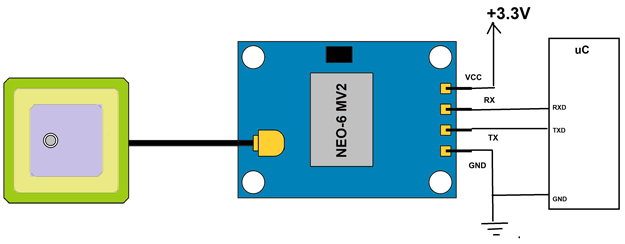
\includegraphics[width=3.125in,height=\textheight]{img/Kampl/GPS-Module-Pins.png}
\caption{GYPINS}
\end{figure}

\hypertarget{kosten}{%
\paragraph{Kosten}\label{kosten}}

\begin{longtable}[]{@{}lllrrr@{}}
\toprule
Anzahl & Ort & Produkt & Einzelpreis & Lieferkosten & Preis
gesamt\tabularnewline
\midrule
\endhead
3 & Ali-Express & GY-NEO6MV2 & 3.19 € & 2.46 € & 12.03 €\tabularnewline
3 & AZ & BME280 & 3.47 € & 5.98 € & 16.39 €\tabularnewline
32 & Reichelt & Lochrasterplatinen & 13.21 € & 6.65 € & 19.86
€\tabularnewline
3 & AZ & GY-521 & 2.50 € & 5.30 € & 12.79 €\tabularnewline
1 & Amazon & ET-Starterkit & 16.13 € & 3.99 € & 20.12 €\tabularnewline
\bottomrule
\end{longtable}

\begin{longtable}[]{@{}l@{}}
\toprule
Preis Hardware insgesamt\tabularnewline
\midrule
\endhead
81.19 €\tabularnewline
\bottomrule
\end{longtable}

\hypertarget{zusammenbau-des-prototyps}{%
\paragraph{Zusammenbau des Prototyps}\label{zusammenbau-des-prototyps}}

Nachdem nun alle Einzelteile vorhanden sind, kann mit dem Zusammenbau
begonnen werden. Bevor jedoch die Komponenten verbunden werden, ist es
wichtig, einen detaillierten Plan zu erstellen. Zur Erstellung dieses
Plans habe ich die Software \textbf{Fritzing} verwendet.

\begin{figure}
\centering
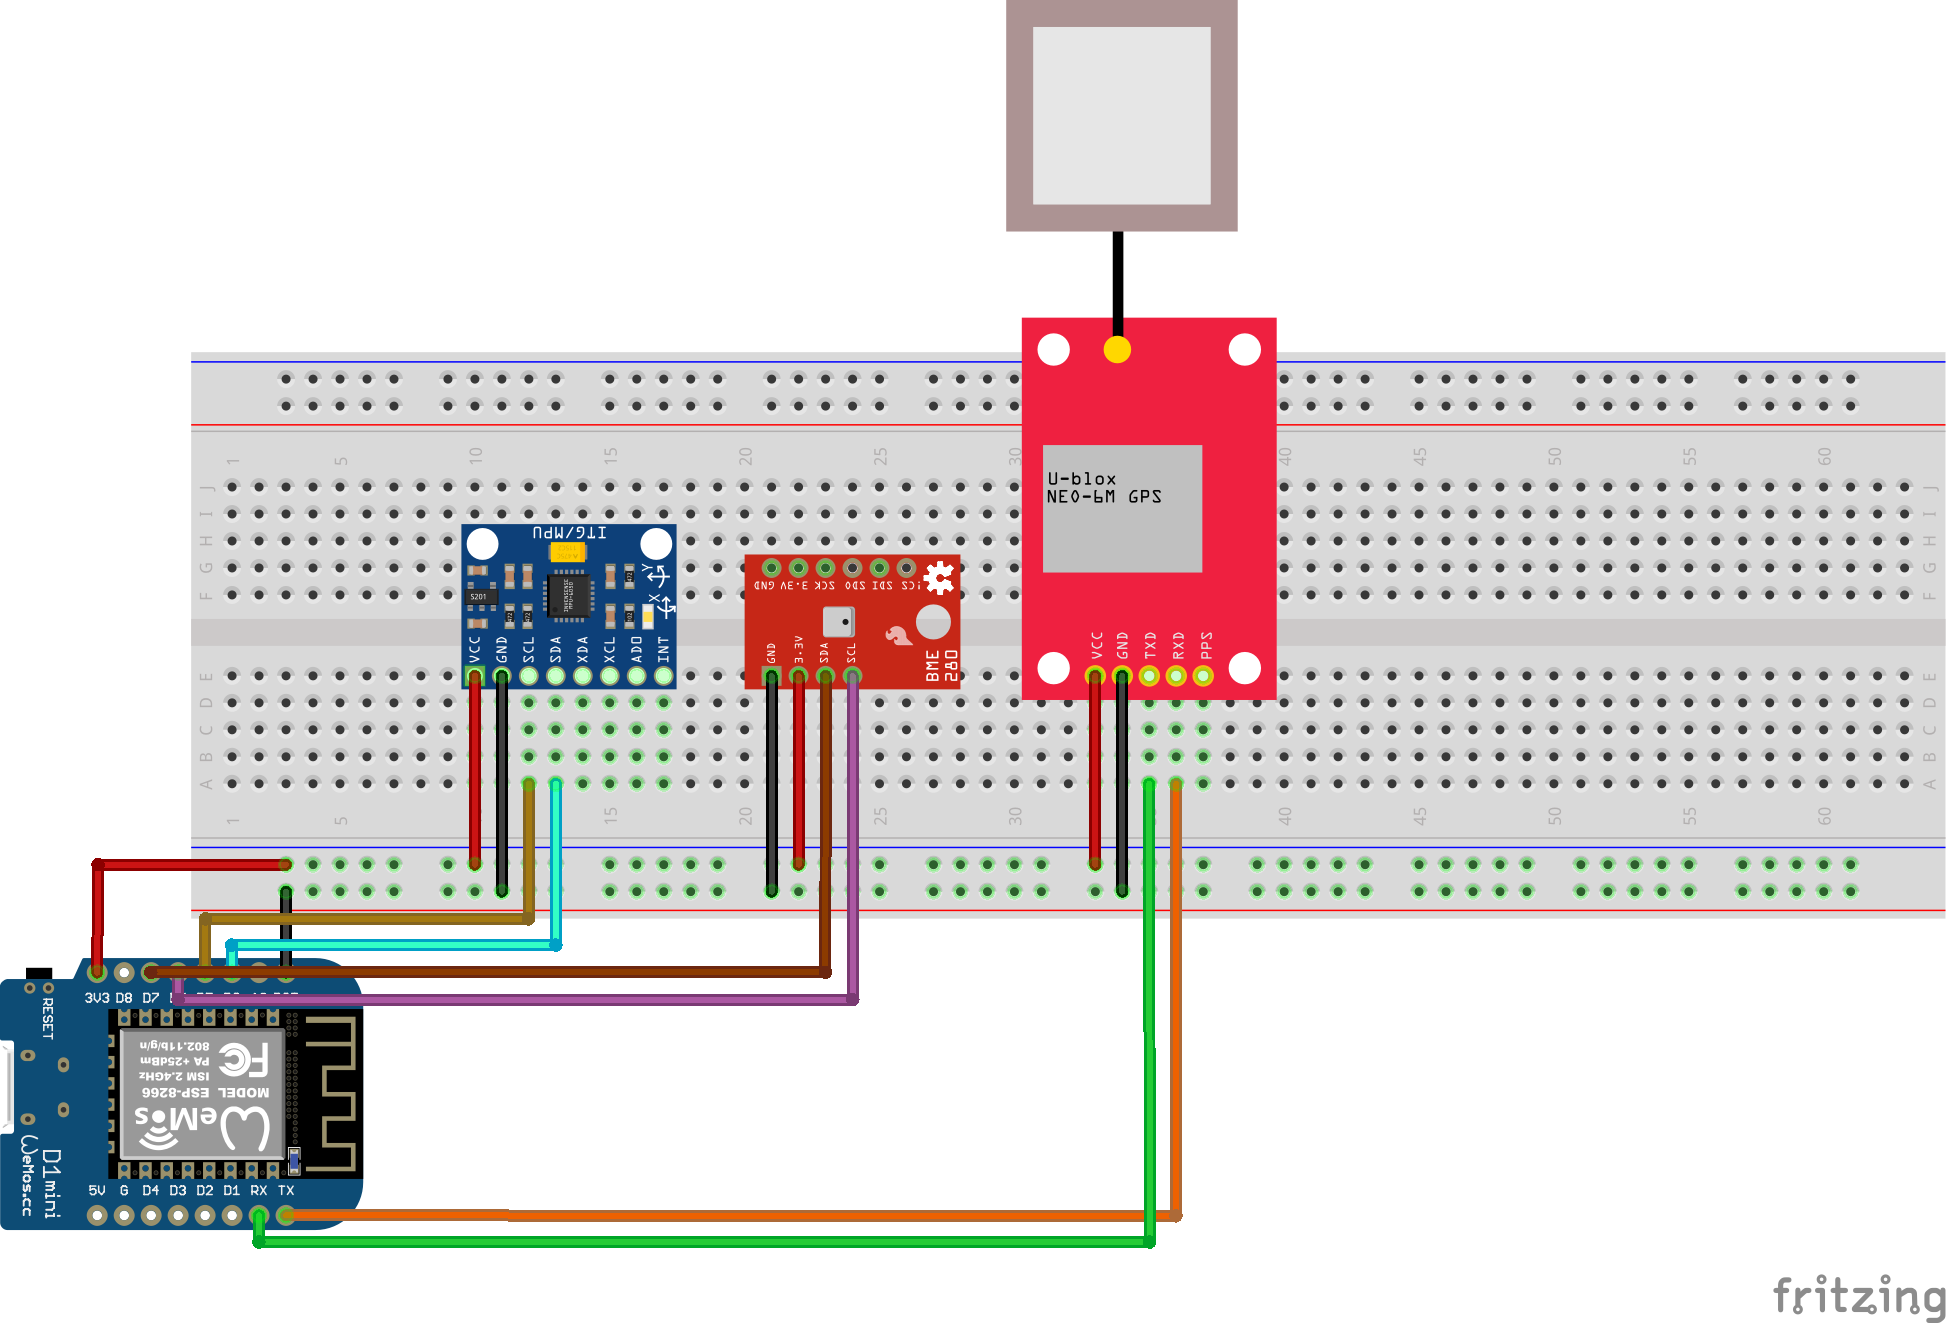
\includegraphics[width=4.16667in,height=\textheight]{img/Kampl/Prototyp-Steckplatine.png}
\caption{Modell des Prototyps}
\end{figure}

\hypertarget{was-ist-fritzing}{%
\subparagraph{Was ist Fritzing?}\label{was-ist-fritzing}}

\begin{quote}
Fritzing ist ein benutzerfreundliches Werkzeug, das einen intuitiven und
nachhaltigen Einstieg in die Elektronik und das Physical Computing
ermöglicht. Die Software stellt elektronische Komponenten wie Sensoren,
Steckplatinen oder Mikrocontroller realistisch dar und erleichtert das
Erstellen von Schaltplänen sowie die Dokumentation elektronischer
Prototypen. Dies schafft eine wichtige Grundlage für die Kommunikation
und den Austausch im Rahmen eines Projekts.
\end{quote}

{[}\protect\hyperlink{ref-Was-ist-Fritzing}{21}{]}

\hypertarget{aufbau-des-prototyps-auf-dem-breadboard}{%
\subparagraph{Aufbau des Prototyps auf dem
Breadboard}\label{aufbau-des-prototyps-auf-dem-breadboard}}

Nach der Modellierung des Grundaufbaus in \textbf{Fritzing} können wir
den Prototypen physisch auf einem \textbf{Breadboard} (Steckplatine)
aufbauen. Dies ist ein wichtiger Schritt, um die einzelnen Komponenten
zu überprüfen und die Programmierung zu starten.

\begin{figure}
\centering
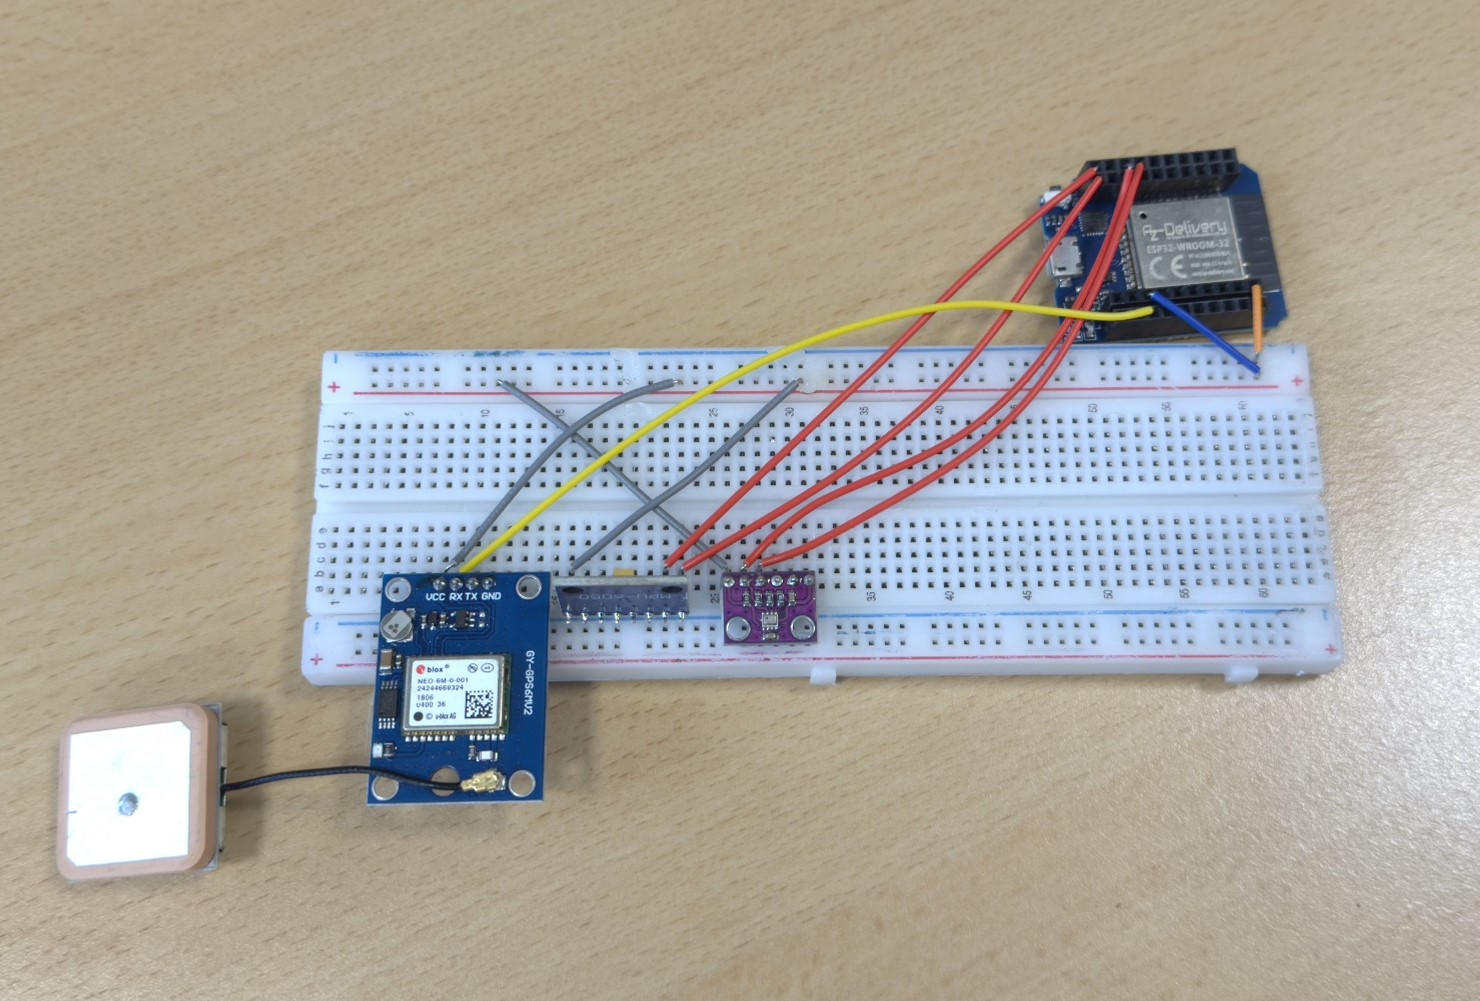
\includegraphics[width=4.16667in,height=\textheight]{img/Kampl/Breadboard-Aufbau.jpg}
\caption{Prototyp auf der Steckplatine}
\end{figure}

\hypertarget{endprodukt}{%
\paragraph{Endprodukt}\label{endprodukt}}

\begin{figure}
\centering
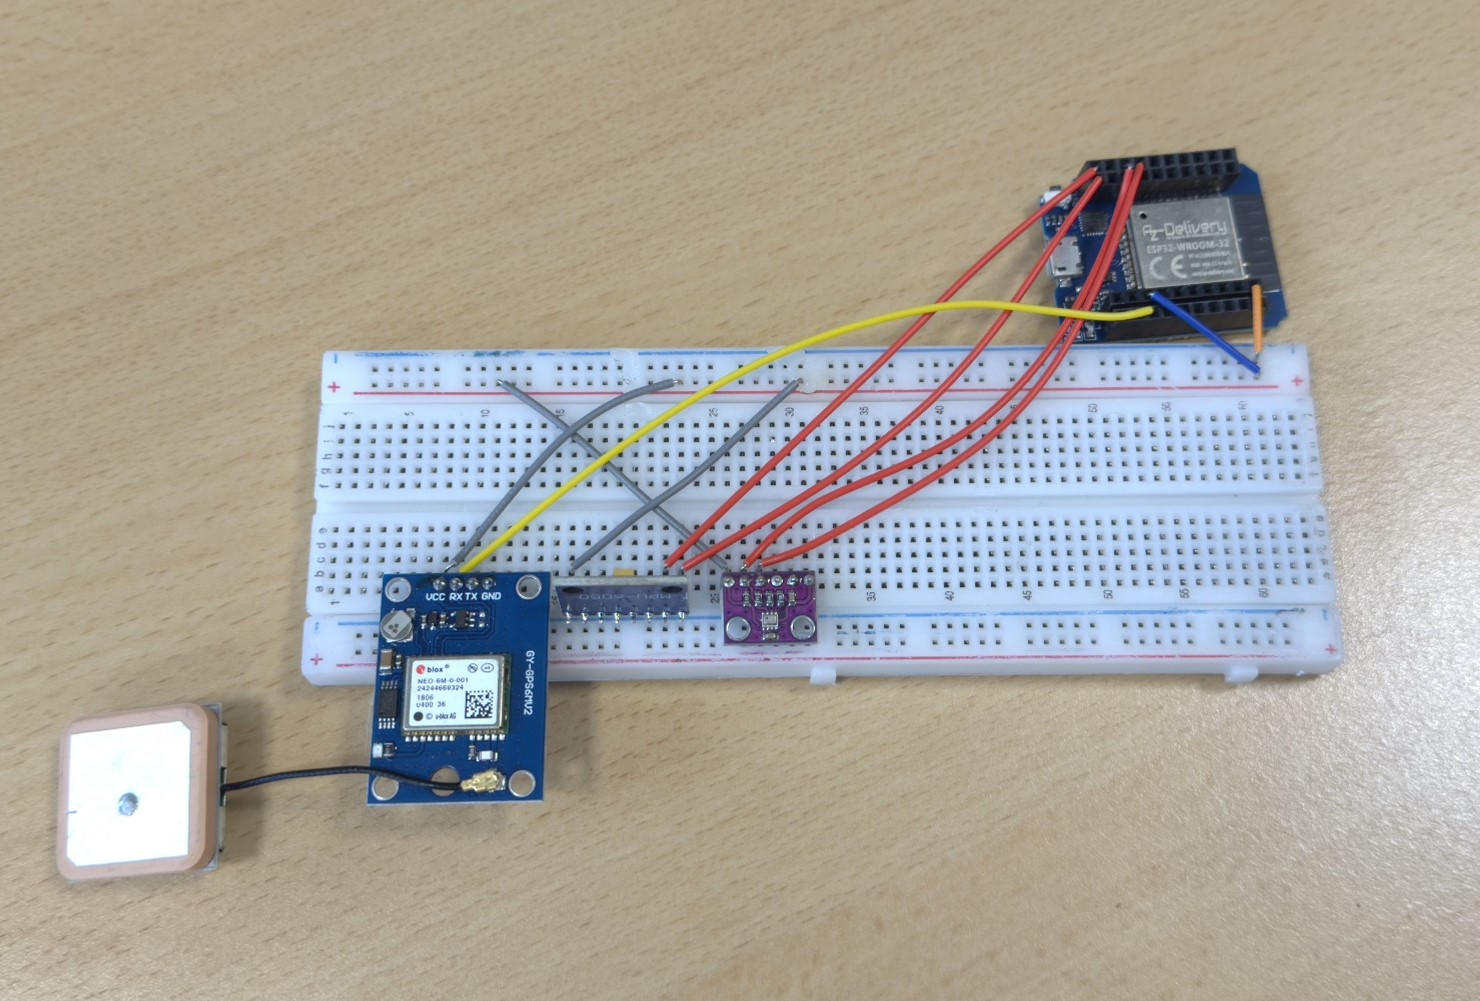
\includegraphics[width=4.16667in,height=\textheight]{img/Kampl/Breadboard-Aufbau.jpg}
\caption{Endprodukt}
\end{figure}

\hypertarget{programmierung-des-prototypen}{%
\subsubsection{Programmierung des
Prototypen}\label{programmierung-des-prototypen}}

Nun, da wir ein vollständig aufgebautes Gerät besitzen, können wir mit
der Programmierung des Prototypen beginnen. Wie bereits in der
theoretischen Ausarbeitung besprochen, verwenden wir hierfür
\textbf{PlatformIO}. Die Initialisierungsdatei sieht wie folgt aus:

\begin{lstlisting}[language={C++}]
; PlatformIO Project Configuration File
;
;   Build options: build flags, source filter
;   Upload options: custom upload port, speed and extra flags
;   Library options: dependencies, extra library storages
;   Advanced options: extra scripting
;
; Bitte besuchen Sie die Dokumentation für weitere Optionen und Beispiele:
; https://docs.platformio.org/page/projectconf.html

[env:esp32dev]
platform = espressif32
board = wemos_d1_mini32
board_build.partitions = min_spiffs.csv
framework = arduino
monitor_speed = 115200
lib_deps = 
    adafruit/Adafruit Unified Sensor@^1.1.14
    adafruit/Adafruit BME280 Library@^2.2.4
    knolleary/PubSubClient@^2.8
    adafruit/Adafruit MPU6050@^2.0.3
    arduino-libraries/Arduino_JSON@^0.1.0
    mikalhart/TinyGPSPlus@^1.1.0
    painlessmesh/painlessMesh@^1.4.5
    ArduinoJson
    arduinoUnity
    TaskScheduler
    AsyncTCP
\end{lstlisting}

In dieser Datei werden viele Konfigurationen festgelegt, damit das
Programm richtig gebaut werden kann. Der verwendete Mikrocontroller ist
der \textbf{wemos\_d1\_mini32}, der auf der Plattform
\textbf{espressif32} basiert. Als Framework wird \textbf{arduino}
verwendet. Die Monitor-Geschwindigkeit ist auf \textbf{115200} Baud
festgelegt. Zudem werden verschiedene Bibliotheken eingebunden, die für
die Funktionalität des Prototypen notwendig sind.

\hypertarget{gesamtes-programm}{%
\paragraph{Gesamtes Programm}\label{gesamtes-programm}}

Im Theorie Teil wurde bereits umfangreich darauf eingegangen, wie die
Programmierung der Sensoren funktioniert, werde ich hier nicht mehr
darauf eingehen, jedoch wurden einige Programmteile noch nicht erklärt
und werden hier aufgeführt. Zuvor jedoch, hier unser Programm welches:

\begin{enumerate}
\def\labelenumi{\arabic{enumi}.}
\tightlist
\item
  Die Daten aus der Sensoren ausliest.
\item
  Die ausgelesenen Daten an den Server mittels MQTT schickt.
\item
  Ein Mesh-Netzwerk benutz, um eine stabile Internetverbindung zu
  bewahren.
\end{enumerate}

\begin{lstlisting}[language={C++}, caption={Ini-File des Prototypen}]
#include "Arduino.h"
#include "Wire.h"
#include "SPI.h"
#include "Adafruit_Sensor.h"
#include "Adafruit_BME280.h"
#include "PubSubClient.h"
#include "WiFi.h"
#include "Adafruit_MPU6050.h"
#include "TinyGPS++.h"
#include "painlessMesh.h"
#include <Arduino_JSON.h>

// Define the RX and TX pins for Serial 2
#define RXD2 16
#define TXD2 17
#define GPS_BAUD 9600

// --- Constants & Credentials ---
const char *ssid = "You lost the Game";
const char *password = "Achtzehn";
const char *mqtt_server = "mqtt.contrude.eu";
const char *mqtt_username = "contrude";
const char *mqtt_password = "HaG1$Vk&62!cWv";
const char *mqtt_domain = "contrude/";
const int ship_number = 1;
const int mqtt_port = 1883;
// Number for this node and also number for the container
int nodeNumber = 1;

String mqtt_publish = String(mqtt_domain) + ship_number + "/" + nodeNumber;

// --- MESH Details ---
#define MESH_PREFIX "CONTRUDE_MESH" 
#define MESH_PORT 5555 

// --- Objects ---
Adafruit_BME280 bme;
Adafruit_MPU6050 mpu;
HardwareSerial gpsSerial(2);
WiFiClient espClient;
PubSubClient client(espClient);
TinyGPSPlus gps;

Scheduler userScheduler;
painlessMesh mesh;


// String to send to other nodes with sensor readings
String readings;

// --- Timing ---
unsigned long currentTime, lastTime = 0;
const unsigned long interval = 1000;

// --- Function Declarations ---
void setup_wifi();
void reconnect();
void publishSensorData();
void printBMEData();
void printMPUData();
void printGPSData();
void initBME();
void initMPU();
void initGPS();
void checkGPS();
String getReadings();
void sendMessage();

// Create tasks: to send messages and get readings
Task taskSendMessage(TASK_SECOND * 5 , TASK_FOREVER, &sendMessage);

String getReadings() {
  JSONVar jsonReadings;
  jsonReadings["node"] = nodeNumber;
  jsonReadings["temp"] = bme.readTemperature();
  jsonReadings["hum"] = bme.readHumidity();
  jsonReadings["pres"] = bme.readPressure()/100.0F;
  readings = JSON.stringify(jsonReadings);
  return readings;
}

void sendMessage() {
  String msg = getReadings();
  mesh.sendBroadcast(msg);
}


void receivedCallback(uint32_t from, String &msg) {
  Serial.printf("Received from %u msg=%s\n", from, msg.c_str());
  JSONVar myObject = JSON.parse(msg.c_str());
  int node = myObject["node"];
  double temp = myObject["temp"];
  double hum = myObject["hum"];
  double pres = myObject["pres"];
  Serial.print("Node: ");
  Serial.println(node);
  Serial.print("Temperature: ");
  Serial.print(temp);
  Serial.println(" C");
  Serial.print("Humidity: ");
  Serial.print(hum);
  Serial.println(" %");
  Serial.print("Pressure: ");
  Serial.print(pres);
  Serial.println(" hpa");
}

void newConnectionCallback(uint32_t nodeId) {
  Serial.printf("New Connection, nodeId = %u\n", nodeId);
}

void changedConnectionCallback() {
  Serial.printf("Changed connections\n");
}

void nodeTimeAdjustedCallback(int32_t offset) {
  Serial.printf("Adjusted time %u. Offset = %d\n", mesh.getNodeTime(), offset);
}

void setup() {
  Serial.begin(115200);

  Serial.println("In Setup");

  // Setup Sensors
  initBME();
  initMPU();
  initGPS();


  // Setup WiFi and MQTT
  setup_wifi();
  client.setServer(mqtt_server, mqtt_port);
  

  //mesh.init(MESH_PREFIX, password, &userScheduler, MESH_PORT);
  //mesh.onReceive(&receivedCallback);
  //mesh.onNewConnection(&newConnectionCallback);
  //mesh.onChangedConnections(&changedConnectionCallback);
  //mesh.onNodeTimeAdjusted(&nodeTimeAdjustedCallback);

  //userScheduler.addTask(taskSendMessage);
  //taskSendMessage.enable();
}

void loop() {
  //mesh.update();

  if (!client.connected()) {
    reconnect();
  }
  client.loop();

  currentTime = millis();
  if (currentTime - lastTime >= interval) {
    publishSensorData();
    printMPUData();
    lastTime = currentTime;
  }
}


// Wifi and Server Segment

void setup_wifi() {
  Serial.print("Connecting to ");
  Serial.println(ssid);
  WiFi.begin(ssid, password);
  while (WiFi.status() != WL_CONNECTED) {
    delay(50);
    Serial.print(".");
  }
  Serial.println("\nWiFi connected!");
}

void reconnect() {
  while (!client.connected()) {
    Serial.print("Attempting MQTT connection...");
    if (client.connect("ESP32Client", mqtt_username, mqtt_password)) {
      Serial.println("connected");
    } else {
      Serial.print("failed, rc=");
      Serial.print(client.state());
      Serial.println(" retrying in 2 seconds...");
      delay(2000);
    }
  }
}

void publishSensorData() {
  sensors_event_t a, g, temp;
  mpu.getEvent(&a, &g, &temp);

  client.publish((String(mqtt_publish) + "/temperature").c_str(), String(bme.readTemperature()).c_str());
  client.publish((String(mqtt_publish) + "/pressure").c_str(), String(bme.readPressure()).c_str());
  client.publish((String(mqtt_publish) + "/humidity").c_str(), String(bme.readHumidity()).c_str());
  client.publish((String(mqtt_publish) + "/vibration").c_str(), String(a.acceleration.x).c_str());



}

// Initializer Segment

void initBME() {
  bme.begin(0x76);
  Serial.println("Initialized BME");
}

void initMPU() {
  mpu.begin();
  Serial.println("Initialized MPU");
}

void initGPS() {
  gpsSerial.begin(GPS_BAUD, SERIAL_8N1, RXD2, TXD2);
  Serial.println("Initialized GPS on Baudrate: " + GPS_BAUD);
}


// Debug Segment 


//void checkGPS() {
//  if (gpsSerial.available() == 0) {
//    Serial.println("No data from GPS module. Check connections.");
//  }
//}
//
void printBMEData() {
  Serial.print("Temperature: ");
  Serial.print(bme.readTemperature());
  Serial.println(" °C");

  Serial.print("Pressure: ");
  Serial.print(bme.readPressure());
  Serial.println(" Pa");

  Serial.print("Humidity: ");
  Serial.print(bme.readHumidity());
  Serial.println(" %");

  Serial.println("---------------------------");
}

void printMPUData() {
  sensors_event_t a, g, temp;
  mpu.getEvent(&a, &g, &temp);

  Serial.print("Acceleration X: ");
  Serial.print(a.acceleration.x);
  Serial.println(" m/s^2");
}

void printGPSData() {
  while (gpsSerial.available() > 0) {
    gps.encode(gpsSerial.read());
  }
}
\end{lstlisting}

\hypertarget{wlan}{%
\paragraph{WLAN}\label{wlan}}

Damit die Daten überhaupt auf den Server geschickt werden können, muss
erst einmal eine Internetverbindung vorliegen. Um diese Verbindung
herzustellen, brauch man den Namen des Netzwerkes die \textbf{ssid} und
das Password. Um nun eine Verbindung aufzubauen muss man dies zwei
Komponenten der WiFi-Bibliothek mittels
\passthrough{\lstinline!WiFi.begin(ssid, password);!} weitergeben. Die
restliche Arbeit erledigt die Bibliothek selbst.

\begin{lstlisting}[language={C++}, caption={Aufbau der WLan Verbindung und Funktion zur Wiederherstellung der Verbindung}]
#include "PubSubClient.h"
#include "WiFi.h"

const char *ssid = "";
const char *password = "";


void setup_wifi() {
  Serial.print("Connecting to ");
  Serial.println(ssid);
  WiFi.begin(ssid, password);
  while (WiFi.status() != WL_CONNECTED) {
    delay(50);
    Serial.print(".");
  }
  Serial.println("\nWiFi connected!");
}
\end{lstlisting}

\hypertarget{mesh}{%
\subparagraph{Mesh}\label{mesh}}

\hypertarget{mqtt-1}{%
\paragraph{MQTT}\label{mqtt-1}}

Wie bereits in der theoretischen Ausarbeitung besprochen, ist MQTT ein
Protokoll zur Übertragung von Daten, bei dem der Publisher, also der
Prototyp, ein Topic abonnieren muss, um genau auf dieses Topic die Daten
zu versenden.

\begin{lstlisting}[language={C++}, caption={Senden der Sensordaten an den MQTT-Server}]
const char *mqtt_server = "mqtt.contrude.eu";
const char *mqtt_username = "contrude";
const char *mqtt_password = "HaG1$Vk&62!cWv";
const char *mqtt_domain = "contrude/";
const int ship_number = 1;
const int mqtt_port = 1883;
// Number for this node and also number for the container
int nodeNumber = 1;

String mqtt_publish = String(mqtt_domain) + ship_number + "/" + nodeNumber;

void publishSensorData() {
  sensors_event_t a, g, temp;
  mpu.getEvent(&a, &g, &temp);

  client.publish((String(mqtt_publish) + "/temperature").c_str(), String(bme.readTemperature()).c_str());
  client.publish((String(mqtt_publish) + "/pressure").c_str(), String(bme.readPressure()).c_str());
  client.publish((String(mqtt_publish) + "/humidity").c_str(), String(bme.readHumidity()).c_str());
  client.publish((String(mqtt_publish) + "/vibration").c_str(), String(a.acceleration.x).c_str());
}

void reconnect() {
  while (!client.connected()) {
    Serial.print("Attempting MQTT connection...");
    if (client.connect("ESP32Client", mqtt_username, mqtt_password)) {
      Serial.println("connected");
    } else {
      Serial.print("failed, rc=");
      Serial.print(client.state());
      Serial.println(" retrying in 2 seconds...");
      delay(2000);
    }
  }
}
\end{lstlisting}

In unserem Fall habe ich das Abonnieren des Topics so skalierbar wie
möglich gemacht. Das bedeutet, dass ich das Topic aufgesplittet habe.

Das eigentliche Topic hat diese Form:
\textbf{contrude/Schiffsnummer/Containernummer/Sensordatenart}.

Um es zu ermöglichen, den Prototypen in jedes Schiff und jeden Container
zu platzieren, habe ich die einzelnen Teile in folgende Variablen
ausgelagert:

\begin{enumerate}
\def\labelenumi{\arabic{enumi}.}
\tightlist
\item
  \passthrough{\lstinline!const char *mqtt\_domain = "contrude/";!}
\item
  \passthrough{\lstinline!const int ship\_number = 1;!}
\item
  \passthrough{\lstinline!const int mqtt\_port = 1883;!}
\item
  \passthrough{\lstinline!int nodeNumber = 1;!}
\end{enumerate}

Diese einzelnen Teile habe ich dann in einem String zusammengefasst:
\passthrough{\lstinline!String mqtt\_publish = String(mqtt\_domain) + ship\_number + "/" + nodeNumber;!}

Die \passthrough{\lstinline!reconnect()!}-Funktion stellt sicher, dass
die Verbindung zum MQTT-Server bei Verbindungsabbrüchen
wiederhergestellt wird.

Falls die Verbindung unterbrochen wird oder der Client nicht verbunden
ist, versucht die Funktion in einer Schleife kontinuierlich, die
Verbindung wieder aufzubauen.

Bei jedem Verbindungsversuch wird überprüft, ob eine erfolgreiche
Verbindung hergestellt werden kann. Falls dies gelingt, wird eine
Bestätigung im Serial-Monitor ausgegeben, andernfalls erfolgt ein neuer
Versuch nach einer Wartezeit von zwei Sekunden. Dieses Verhalten
gewährleistet eine zuverlässige Datenübertragung, auch bei
Netzwerkproblemen oder Neustarts des Geräts. \# Teilaufgabe Schüler
Schrempf

\textauthor{Marko Daniel Schrempf}

\hypertarget{theorie-1}{%
\subsection{Theorie}\label{theorie-1}}

\hypertarget{datenspeicherung-und-visualisierung}{%
\subsubsection{Datenspeicherung und
Visualisierung}\label{datenspeicherung-und-visualisierung}}

Eine Datenbank ermöglicht die Speicherung und Verwaltung von
zusammenhängenden Daten. Hier können große Datenmengen übersichtlich
abgebildet werden. Es gibt verschiedenste Datenbankkonzepte, welche auf
ihre eigene Art und Weise Vor- und Nachteile bringen. In dieser
Ausarbeitung wird sich auf zwei funktional unterschiedliche Arten
fokussiert.

\hypertarget{relationale-datenbanken}{%
\paragraph{Relationale Datenbanken}\label{relationale-datenbanken}}

In einem relationalen Datenbanksystem werden Daten in Form von Tabellen
gespeichert. Jede Tabelle hat eine Relation zu einer anderen Tabelle,
entweder inhaltich oder strukturell. Durch diese Beziehungen, wenn sie
richtig definiert sind, werden Redundanzen vermieden. Um solche
Beziehungen richtig aufzubauen gibt es das Konzept der Normalisierung.

\begin{quote}
Die Normalisierung von relationalen Datenbanken ist ein Vorgehen, bei
dem die Ausgangstabelle in mehrere kleine Tabellen zerlegt wird. Dann
werden sie über Fremdschlüssel in Beziehung gesetzt. Ziel einer solchen
Normalisierung ist das Erschaffen einer redundanzfreien
Datenspeicherung, die Vermeidung von Anomalien, sowie die Erstellung
eines klar strukturierten Datenbankmodells.
{[}\protect\hyperlink{ref-Nachhilfe-Team}{22}{]}
\end{quote}

Der entscheidende Vorteil von RDBs\footnote{Relationale Datenbank} ist,
dass sie eine gemeinsame standardisierte Sprache für die Datenabfrage-
und verarbeitung besitzen - SQL\footnote{Structured Query Language}. In
relationalen Datenbanken werden primär Informationen persistiert, welche
auf längere Zeit vorhanden bleiben und auf die nicht in kurzen
Zeitintervallen zugegriffen wird.

\hypertarget{zeitreihen-datenbanken}{%
\paragraph{Zeitreihen Datenbanken}\label{zeitreihen-datenbanken}}

In einem zeitreihen basierten Datenbanksystem werden Daten mit einem
korrespondierenden Zeitstempel versehen. In anderen Datenbanken ist das
Speichern einer Zeitmarke per Wert zwar auch möglich, jedoch weist eine
TSDB\footnote{Time Series Database} jedem einzelnen Wert automatisch
einen eindeutigen Timestamp zu und vermerkt den daraus resultierenden
Datensatz in einer Historie. In dieser ist der gesamte zeitliche Verlauf
des Attributs festgehalten.

Zeitreihen DBs\footnote{Datenbank} sind optimiert auf viele schreib und
lese Operationen und sind nicht auf das verändern bzw. löschen der
Datensätze ausgelegt. Je nach DBMS\footnote{Datenbankmanagementsystem}
können verschiedene Erfassungszeiträume und somit auch die Granularitiät
des Timestamps definiert werden. Dies kann von Millisekunden bis hin zu
Tagen gehen. Außerdem gibt es keine einheitliche Query-Sprache. In TSDBs
werden Metriken, Sensordaten und generell Werte mit hoher Änderungsrate
persistiert. {[}\protect\hyperlink{ref-Computerweekly}{23}{]}

Ein Sonderfall der TSDB ist die RRD\footnote{Round Robin Database}.
Diese löscht alte Datensets nach einer definierten Zeit und / oder
aggregiert sie auf einen Wert zusammen.
{[}\protect\hyperlink{ref-joojscript}{24}{]}

\hypertarget{visualisierung}{%
\paragraph{Visualisierung}\label{visualisierung}}

\begin{quote}
Datenvisualisierung ist der Prozess der Verwendung visueller Elemente
wie Diagramme, Grafiken oder Karten zur Darstellung von Daten. Sie
übersetzt komplexe, umfangreiche oder numerische Daten in eine visuelle
Darstellung, die leichter zu verarbeiten ist.
{[}\protect\hyperlink{ref-aws-datenvisualisierung}{25}{]}
\end{quote}

Um Rohdaten verständlich zu machen, im Kontext betrachten zu können und
etwaige Korrelationen zwischen verschiedenen Datensets sichtbar zu
machen, ist es notwendig, die oben genannten Methoden anzuwenden.
Hierbei ist eine unkomplizierte Grafik als Endprodukt das Ziel.

\begin{figure}
\centering
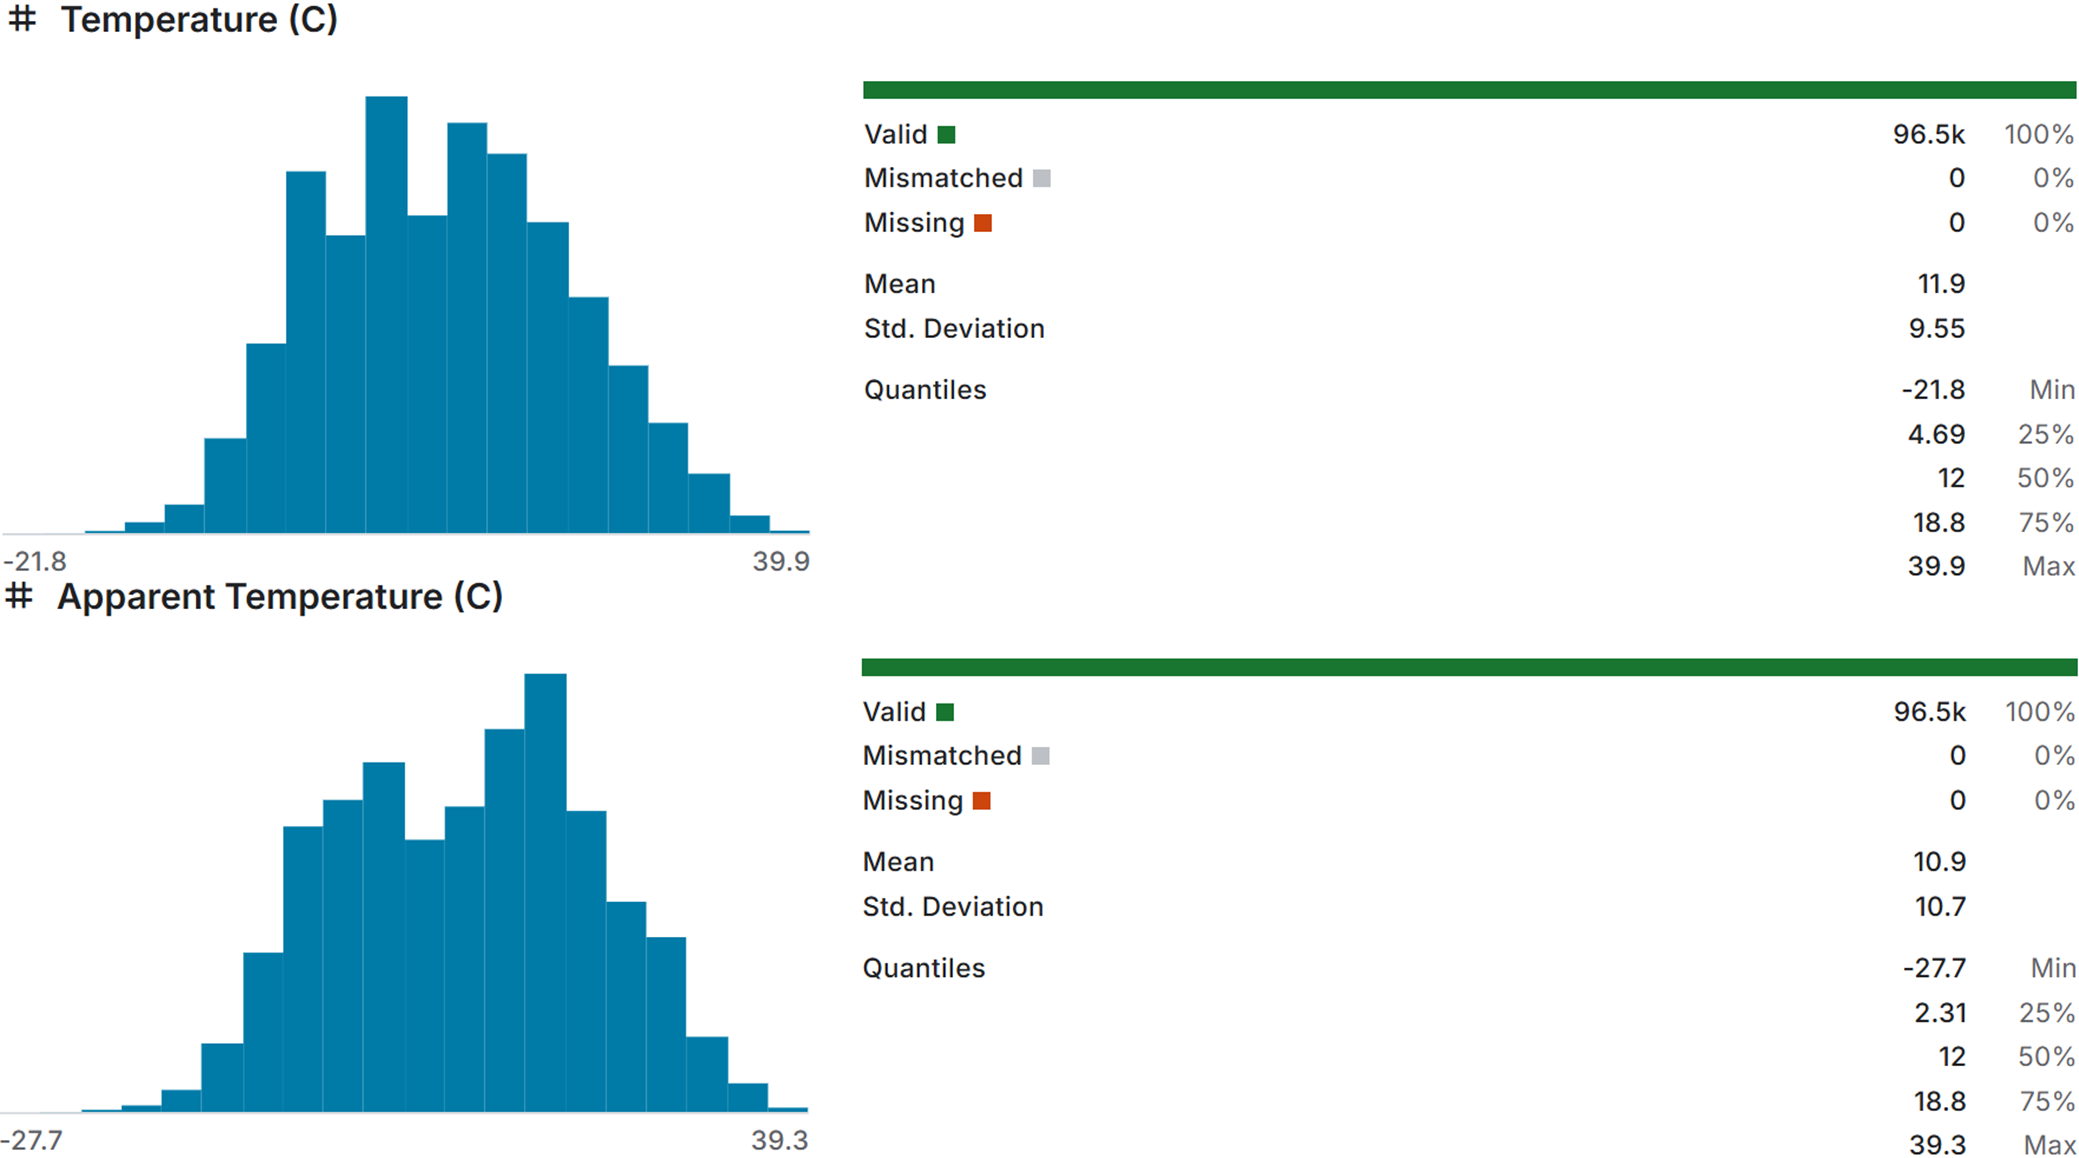
\includegraphics[width=1\textwidth,height=\textheight]{img/Schrempf/weather-data-set.png}
\caption{Beispiel einer Datenvisualisierung von Mittelwerten einer
Temperaturaufzeichnung
{[}\protect\hyperlink{ref-kaggle-weather-data}{26}{]}}
\end{figure}

Um solch ein Ergebnis zu erreichen, müssen vorhandene Daten bereinigt,
gefiltert und ausgewählt werden. Beim Erstellen der Visualisierungen
muss eine Verzerrung der Daten hinsichtlich Trivialisierung,
Überspitzung und menschlichen Vorurteilen vermeiden werden.
{[}\protect\hyperlink{ref-aws-datenvisualisierung}{25}{]}

\hypertarget{datenuxfcbertragung-1}{%
\subsubsection{Datenübertragung}\label{datenuxfcbertragung-1}}

\hypertarget{reverse-proxy}{%
\paragraph{Reverse Proxy}\label{reverse-proxy}}

Ein Reverse Proxy ist zwischen den in das Internet freigeschaltenen
Services und dem Internet. Somit kommuniziert ein Client nicht direkt
mit den Services, sondern muss zuerst beim Reverse Proxy vorbei. Dies
hat mehrere Vorteile. Die Anwendungen sind nicht direkt dem Internet
ausgesetzt, was eine zusätzliche Sicherheitsebene einführt, da nie die
Server IP(s), sondern nur die des Reverse Proxies ersichtlich sind. Load
Balancing ist ein weiterer Aspekt einer solchen Software. Es beschreibt
den Vorgang des Aufteilens der Anfragen an verschiedene Server, die aber
nach außen hin als einer agieren. Somit können überlastungsbedingte
Ausfälle vermieden werden. Wenn mehrere Benutzer den gleichen Inhalt
abfragen wollen, kann dieser zur Leistungsverbesserung
zwischengespeichert werden - Caching genannt. Diese Tätigkeit kann auch
übernommen werden. {[}\protect\hyperlink{ref-reverse-proxy}{27}{]}

\begin{figure}
\centering
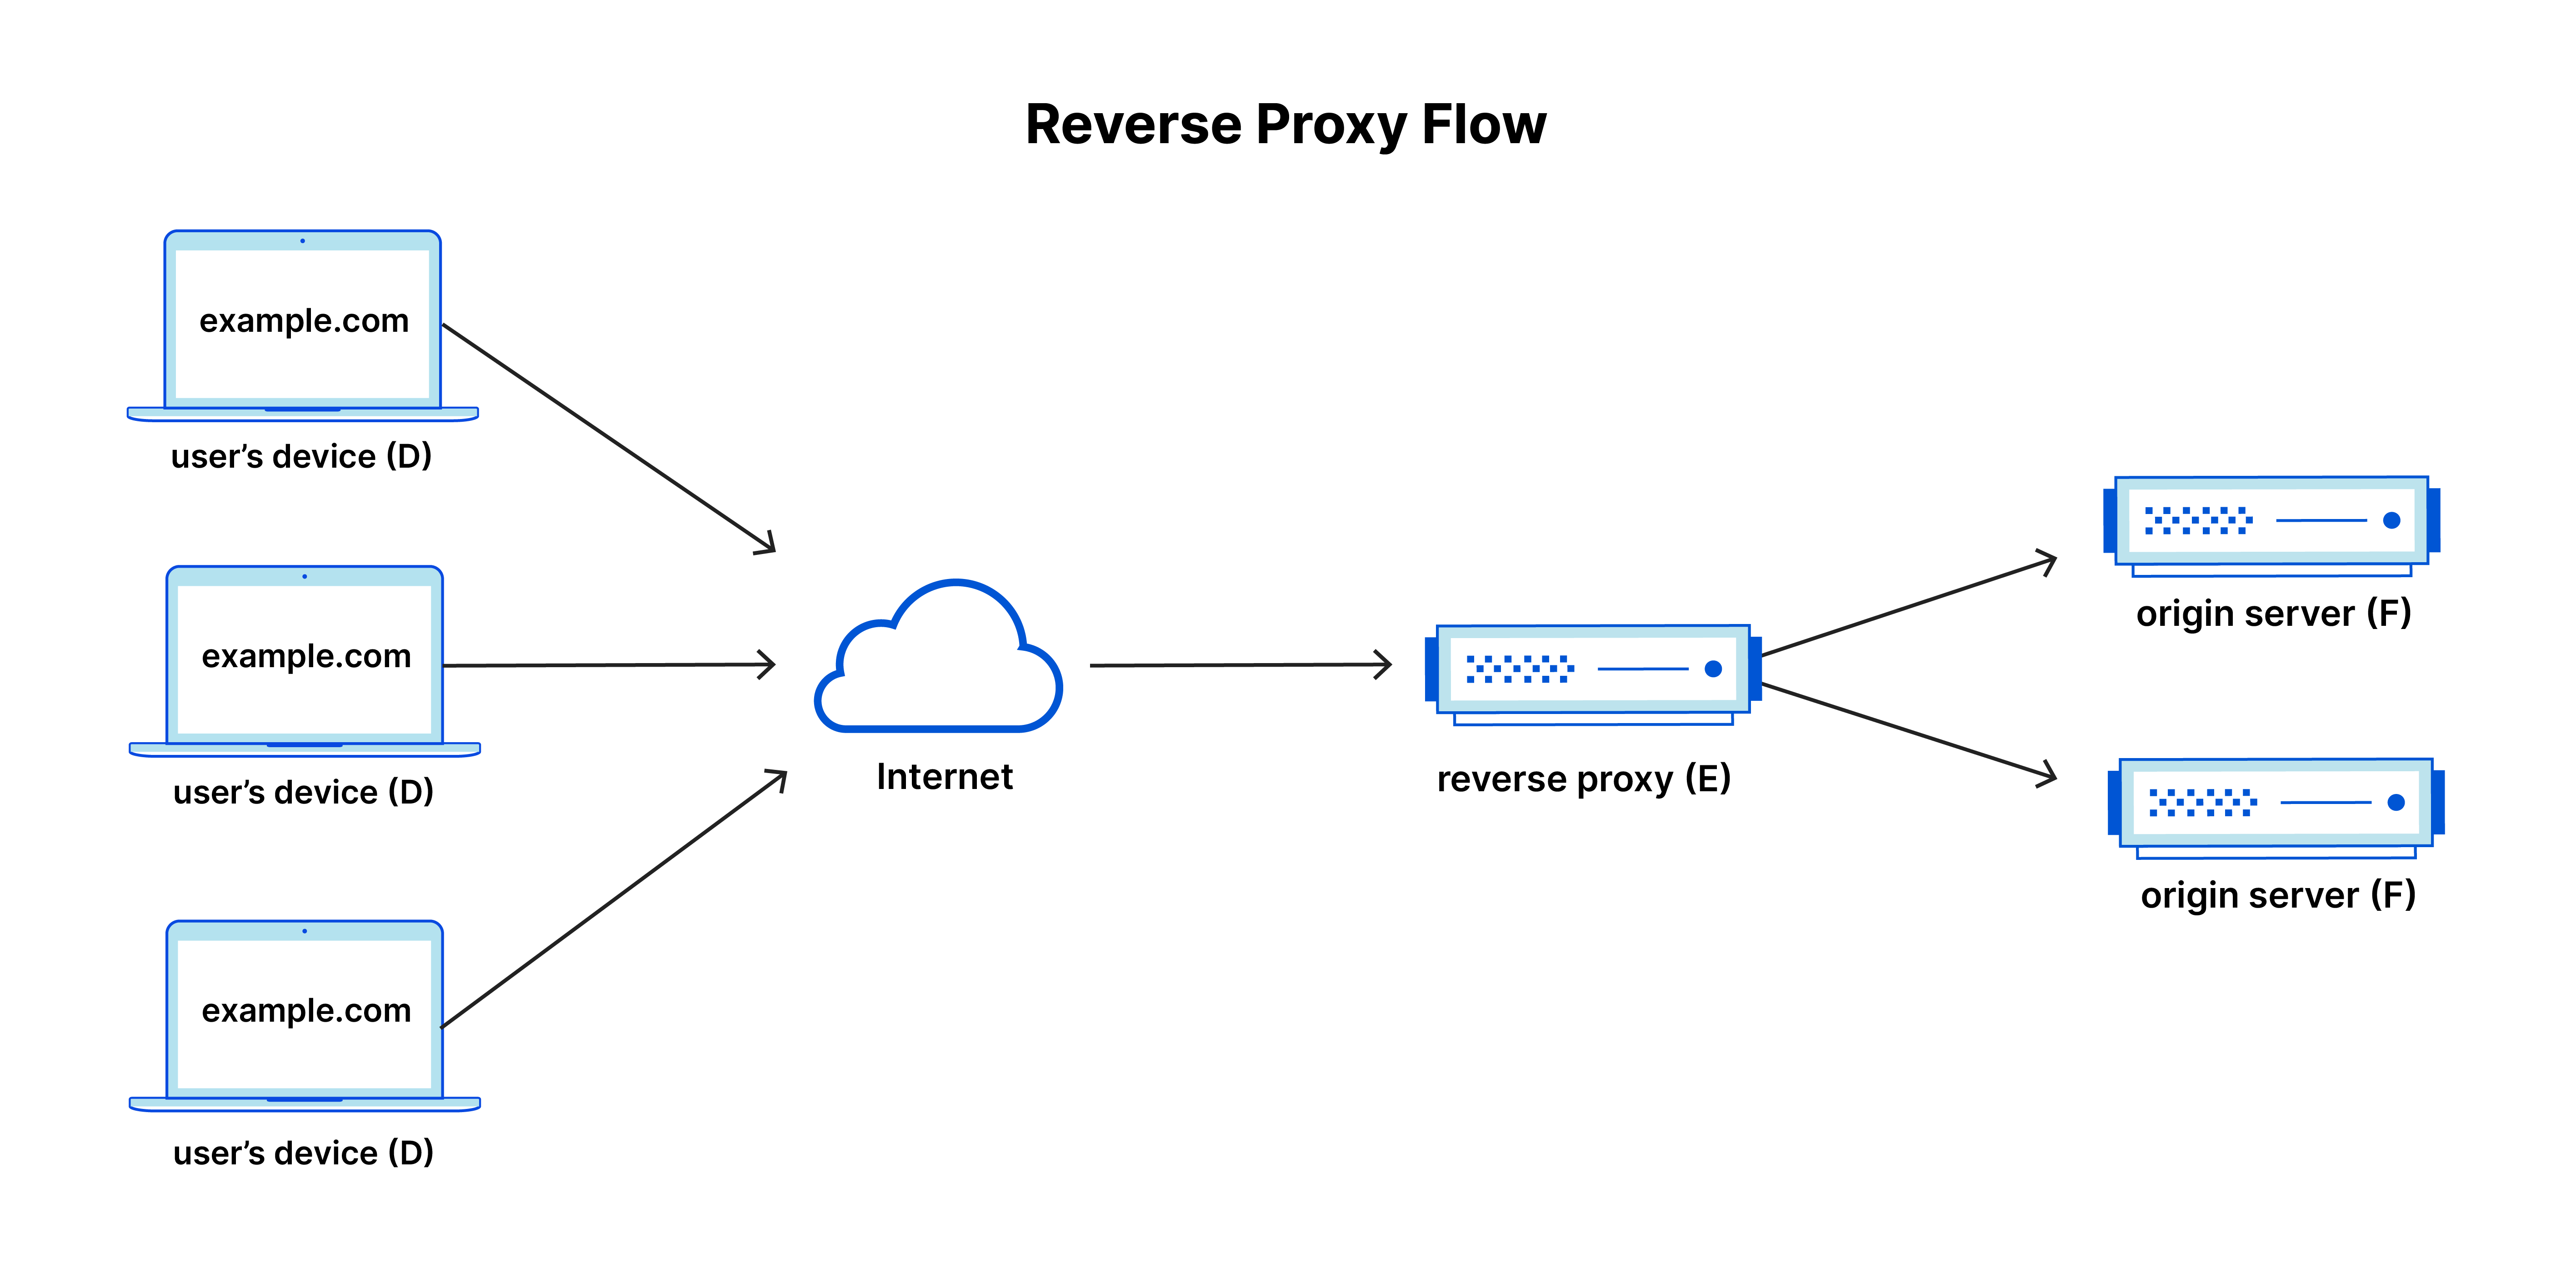
\includegraphics[width=1\textwidth,height=\textheight]{img/Schrempf/reverse-proxy.png}
\caption{Funktionsweise eines Reverse Proxies
{[}\protect\hyperlink{ref-tls}{28}{]}}
\end{figure}

Niemand will seine Daten unverschlüsselt versenden. Eine oft in
Kombination angebotene Lösung: SSL\footnote{Secure Sockets Layer} bzw.
TLS\footnote{Transport Layer Security}.
{[}\protect\hyperlink{ref-reverse-proxy}{27}{]} SSL ist der namentliche
Vorgänger zu TLS und ermöglicht das S in HTTPS\footnote{Hypertext
  Transfer Protocol Secure}. Bei SSL wird ein Handshake zwischen den
Geräten durchgeführt, welcher beweisen soll, dass sie auch die sind, für
die sie sich ausgeben. Außerdem werden die Daten verschlüsselt und
digital signiert. TLS hieß es erst seit dem, dass nicht nur die
IETF\footnote{Internet Engineering Task Force} sondern auch Netscape
daran mitentwickelten. Beide funktionieren mit einem Asymmetrisches
Kryptosystem. {[}\protect\hyperlink{ref-ssl}{29}{]}
{[}\protect\hyperlink{ref-tls}{28}{]}

\begin{figure}
\centering
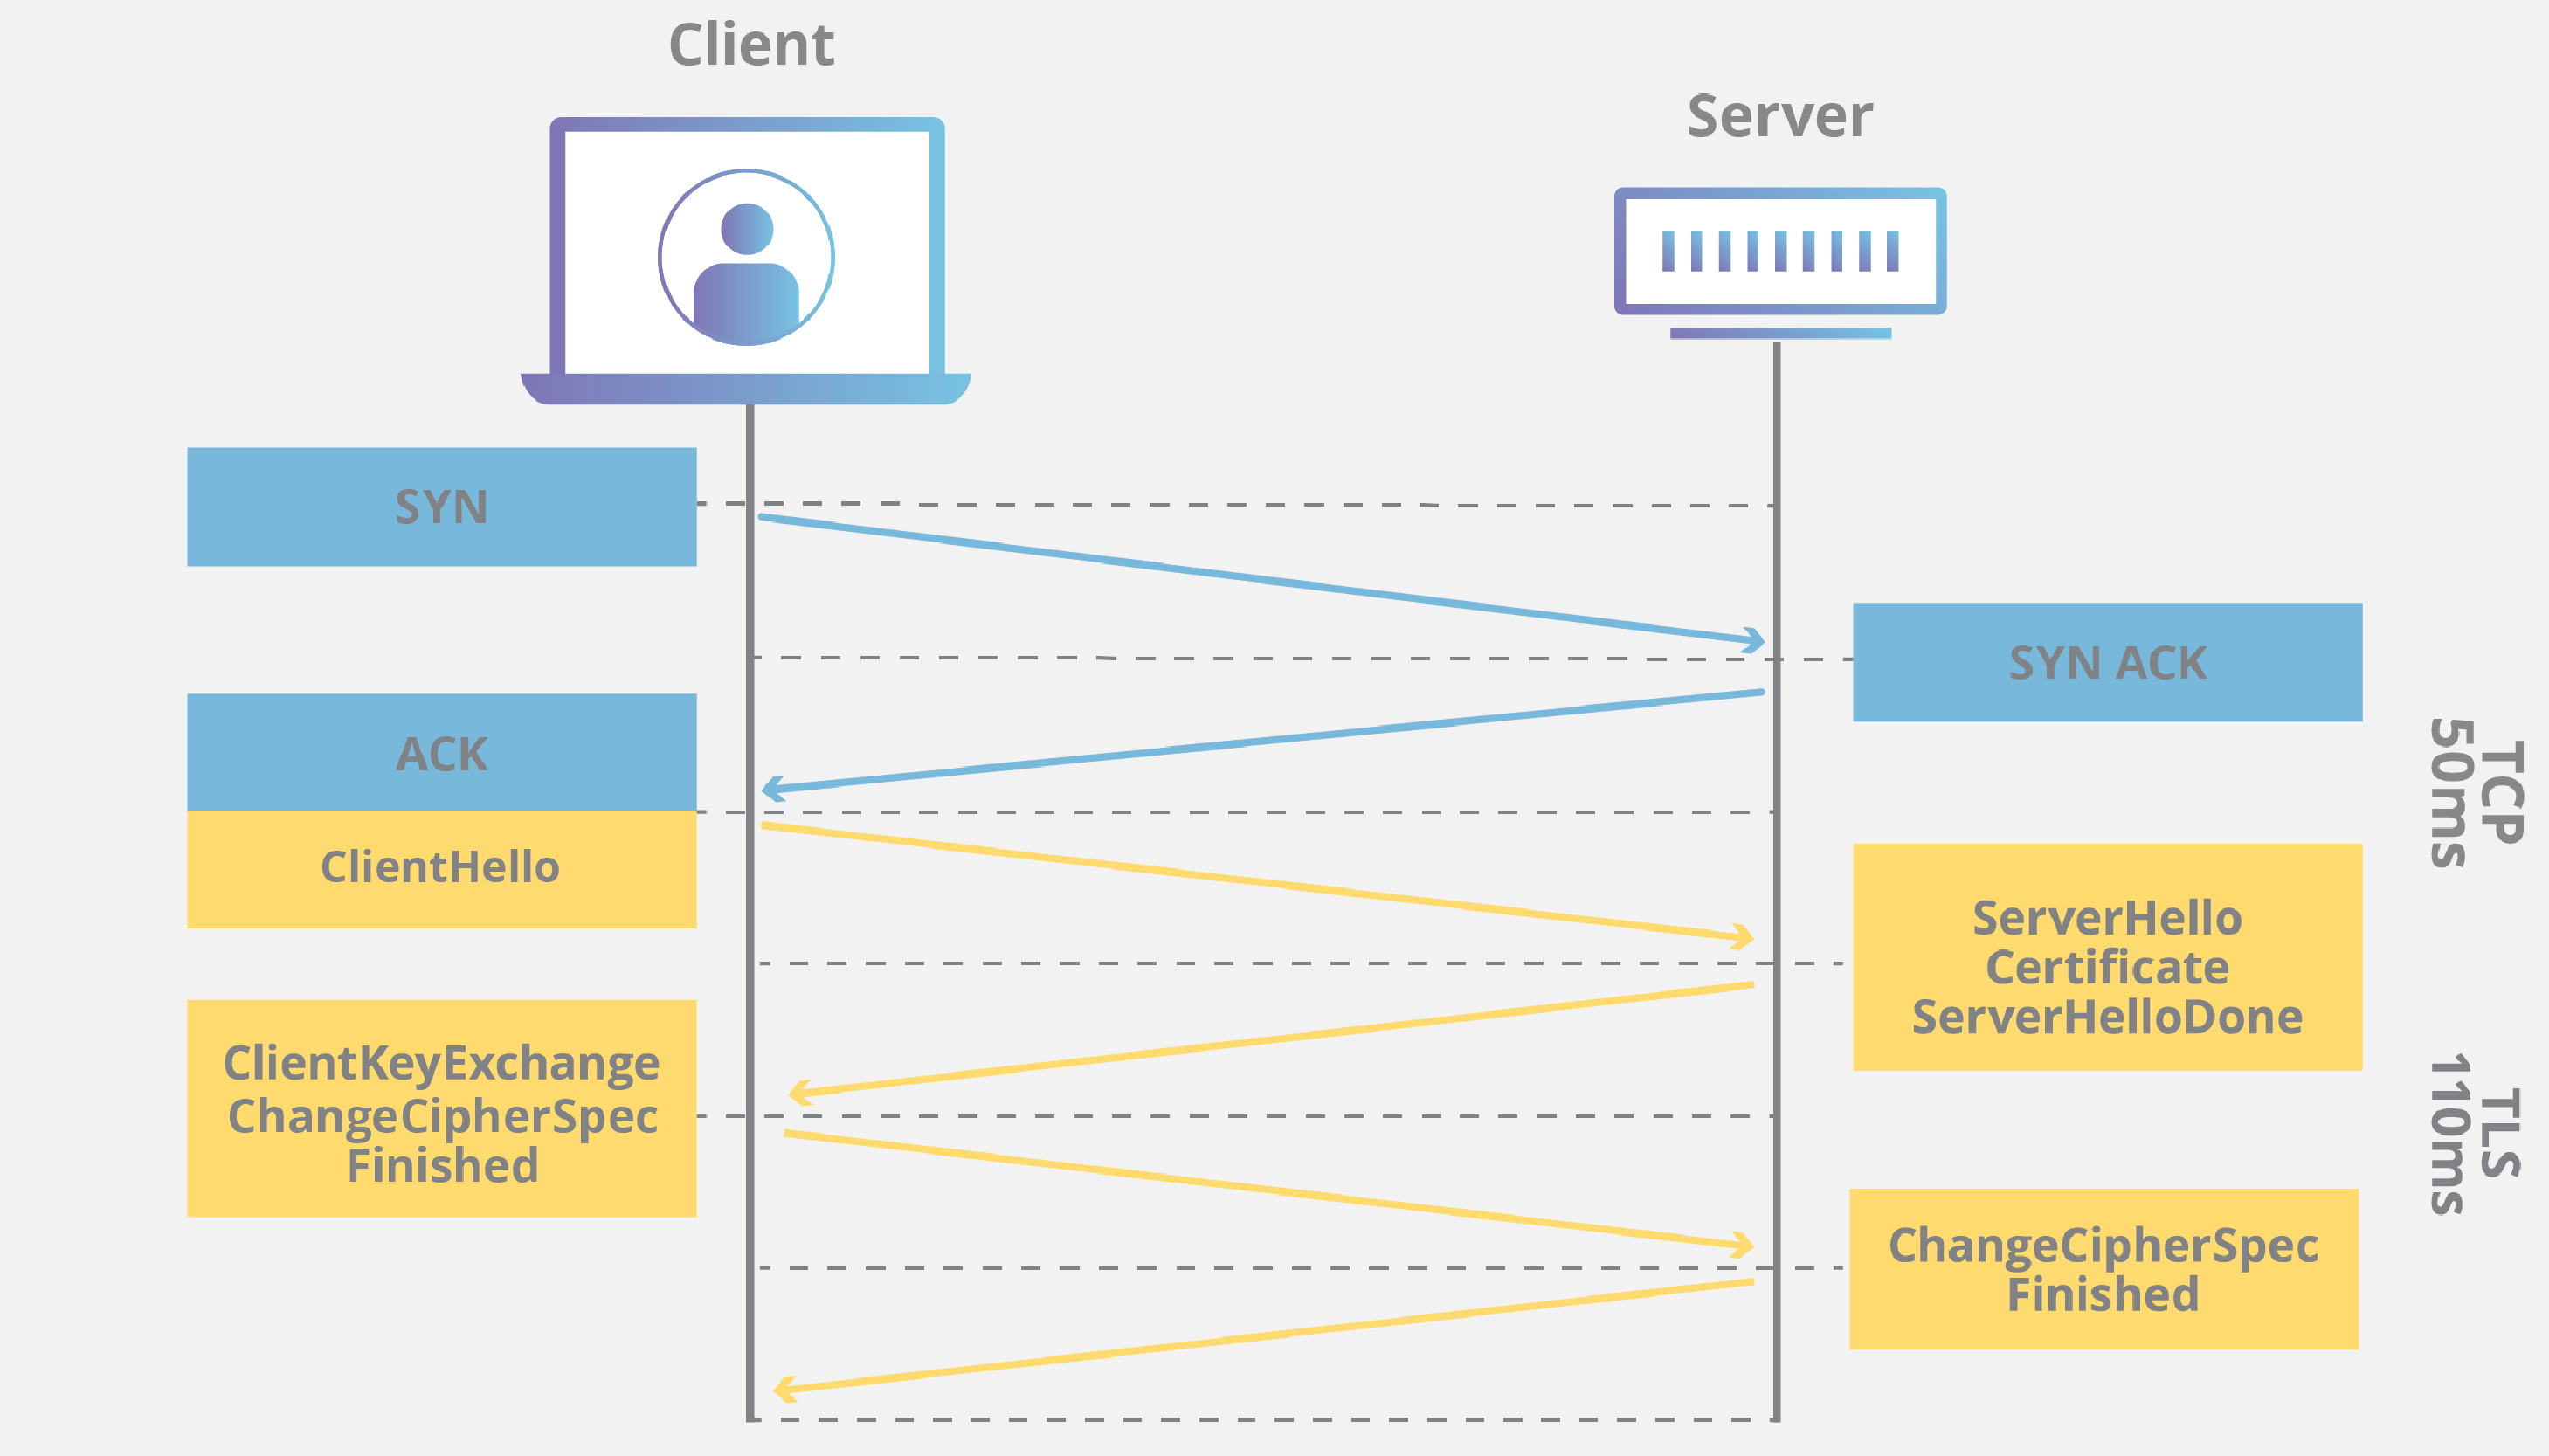
\includegraphics[width=1\textwidth,height=\textheight]{img/Schrempf/tls-ssl-handshake.png}
\caption{Funktionsweise eines TLS Handshakes
{[}\protect\hyperlink{ref-tls}{28}{]}}
\end{figure}

\hypertarget{mqtt-2}{%
\paragraph{MQTT}\label{mqtt-2}}

MQTT\footnote{Message Queuing Telemetry Transport} ist ein
Nachrichtenprotokoll, welches dazu verwendet wird, um mit nicht stabilen
Netzwerken oder mit Netzwerken mit begrenzten Ressourcen zu
kommunizieren. Dieser basiert auf der Publisher-Subscriber Architektur.
Der Publisher sendet seine Daten and den Broker unter einem gewissen
Topic. Diese kann man semantisch aneinanderreihen um Subkategorien eines
Themas zu erstellen. Man kann es sich als eine Baumstruktur vorstellen.
Für ein komplett neues Thema wird ein neues Topic erstellt. Hierbei ist
zu beachten, dass ein \# als Platzhalter inmitten eines Pfades dienen
kann. Ein Beispiel für solch eine Baumstruktur ist
\passthrough{\lstinline!town/house/kitchen!}. Unter diesem Topic kann
nun ein oder mehrere Werte im JSON\footnote{JavaScript Object Notation}-Format
abgelegt werden. Beim Broker liegen dann die Werte auf. Ein Topic kann
auch einen oder mehrere Tags haben. Diese sind Flags, welche zur
weiteren Klassifizierung des Topics an es angehängt werden können. Ein
Subscriber ist ein beliebiger Akteur, welcher den abgespeicherten
Datensatz unter der Angabe des Topics extrahiert.
{[}\protect\hyperlink{ref-mqtt-hivemq}{30}{]}

\begin{figure}
\centering
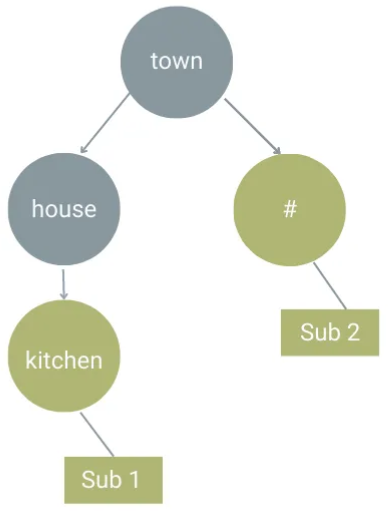
\includegraphics[width=0.3\textwidth,height=\textheight]{img/Schrempf/mqtt-topic-structure.png}
\caption{Beispiel MQTT Topic Structure
{[}\protect\hyperlink{ref-mqtt-hivemq}{30}{]}}
\end{figure}

\hypertarget{json-web-token}{%
\paragraph{JSON Web Token}\label{json-web-token}}

JWTs\footnote{JSON Web Token} sind mit dem Standard RFC 7519 normiert.
Sie dienen dazu, Tokens, also Schlüssel, zur Authentifizierung zu
erstellen. Sie sind sehr kompakt und können deshalb gut in HTTP-Headers
transportiert werden und enthalten Informationen zu den betroffenen
Benutzern. Durch die in ihnen gespeicherten Informationen vermindert man
die Anfragen, welche an die Datenbanken gestellt werdene müssen. Sie
werden dafür genutzt, um den Zugriff zu Diensten zu regulieren oder
verschlüsselt Daten auszutauschen. {[}\protect\hyperlink{ref-jwt}{31}{]}

Ein JSON Web Token besteht aus drei Teilen, welche durch Punkte getrennt
werden und im Base64 Format vorliegen. Der Header, Payload und die
Signatur. Somit folgt dieser Token der Form
\passthrough{\lstinline!xxxxx.yyyyy.zzzzz!}. Im Header wird der Typ des
Tokens (JWT) und der benutzte Hashingalgorithmus angegeben. In der
Payload werden die zu haltenden Daten angegeben. Die Signatur dient
dazu, zu verifizieren, dass der Absender / Ersteller des Tokens der ist,
für den er sich ausgibt. Sie besteht aus dem gehashten addierten Werten
des Headers, Payloads und eines Secrets. Das Secret dient als eine Art
Salt, welches zur Garantie der Eindeutigkeit beigefügt wird. Ein Salt
ist ein Zeichenkette, welche der Hashalgorithmus mathematisch
verschränkt in das Endprodukt einbindet.
{[}\protect\hyperlink{ref-jwt}{31}{]}

\begin{lstlisting}[caption={HMAC SHA256 Signatur eines JWT}]
HMACSHA256(
  base64UrlEncode(header) + '.' +
  base64UrlEncode(payload),
  secret)
\end{lstlisting}

Wie funktioniert es? Am Anfang gibt der Benutzer sein Login Daten an.
Vorzugsweise Benutzername und Passwort. Nun wird ihm nach erfolgreicher
Authentifizierung der Token zurückgegeben, welchen er bei den Protected
Routes im Authentication Header der Anfrage mitführen muss. Ein JWT ist
stateless, was bedeutet, dass der Status des Benutzers nicht im Server
vermerkt ist. {[}\protect\hyperlink{ref-jwt}{31}{]} Da solch ein Token
eine gewisse Macht mit sich bringt, ist stets zu beachten, dass die
Tokens auch nur eine gewisse Zeit, meistens 10 - 15 min gültig sind.
{[}\protect\hyperlink{ref-medium-auth-simple}{32}{]}

\begin{figure}
\centering
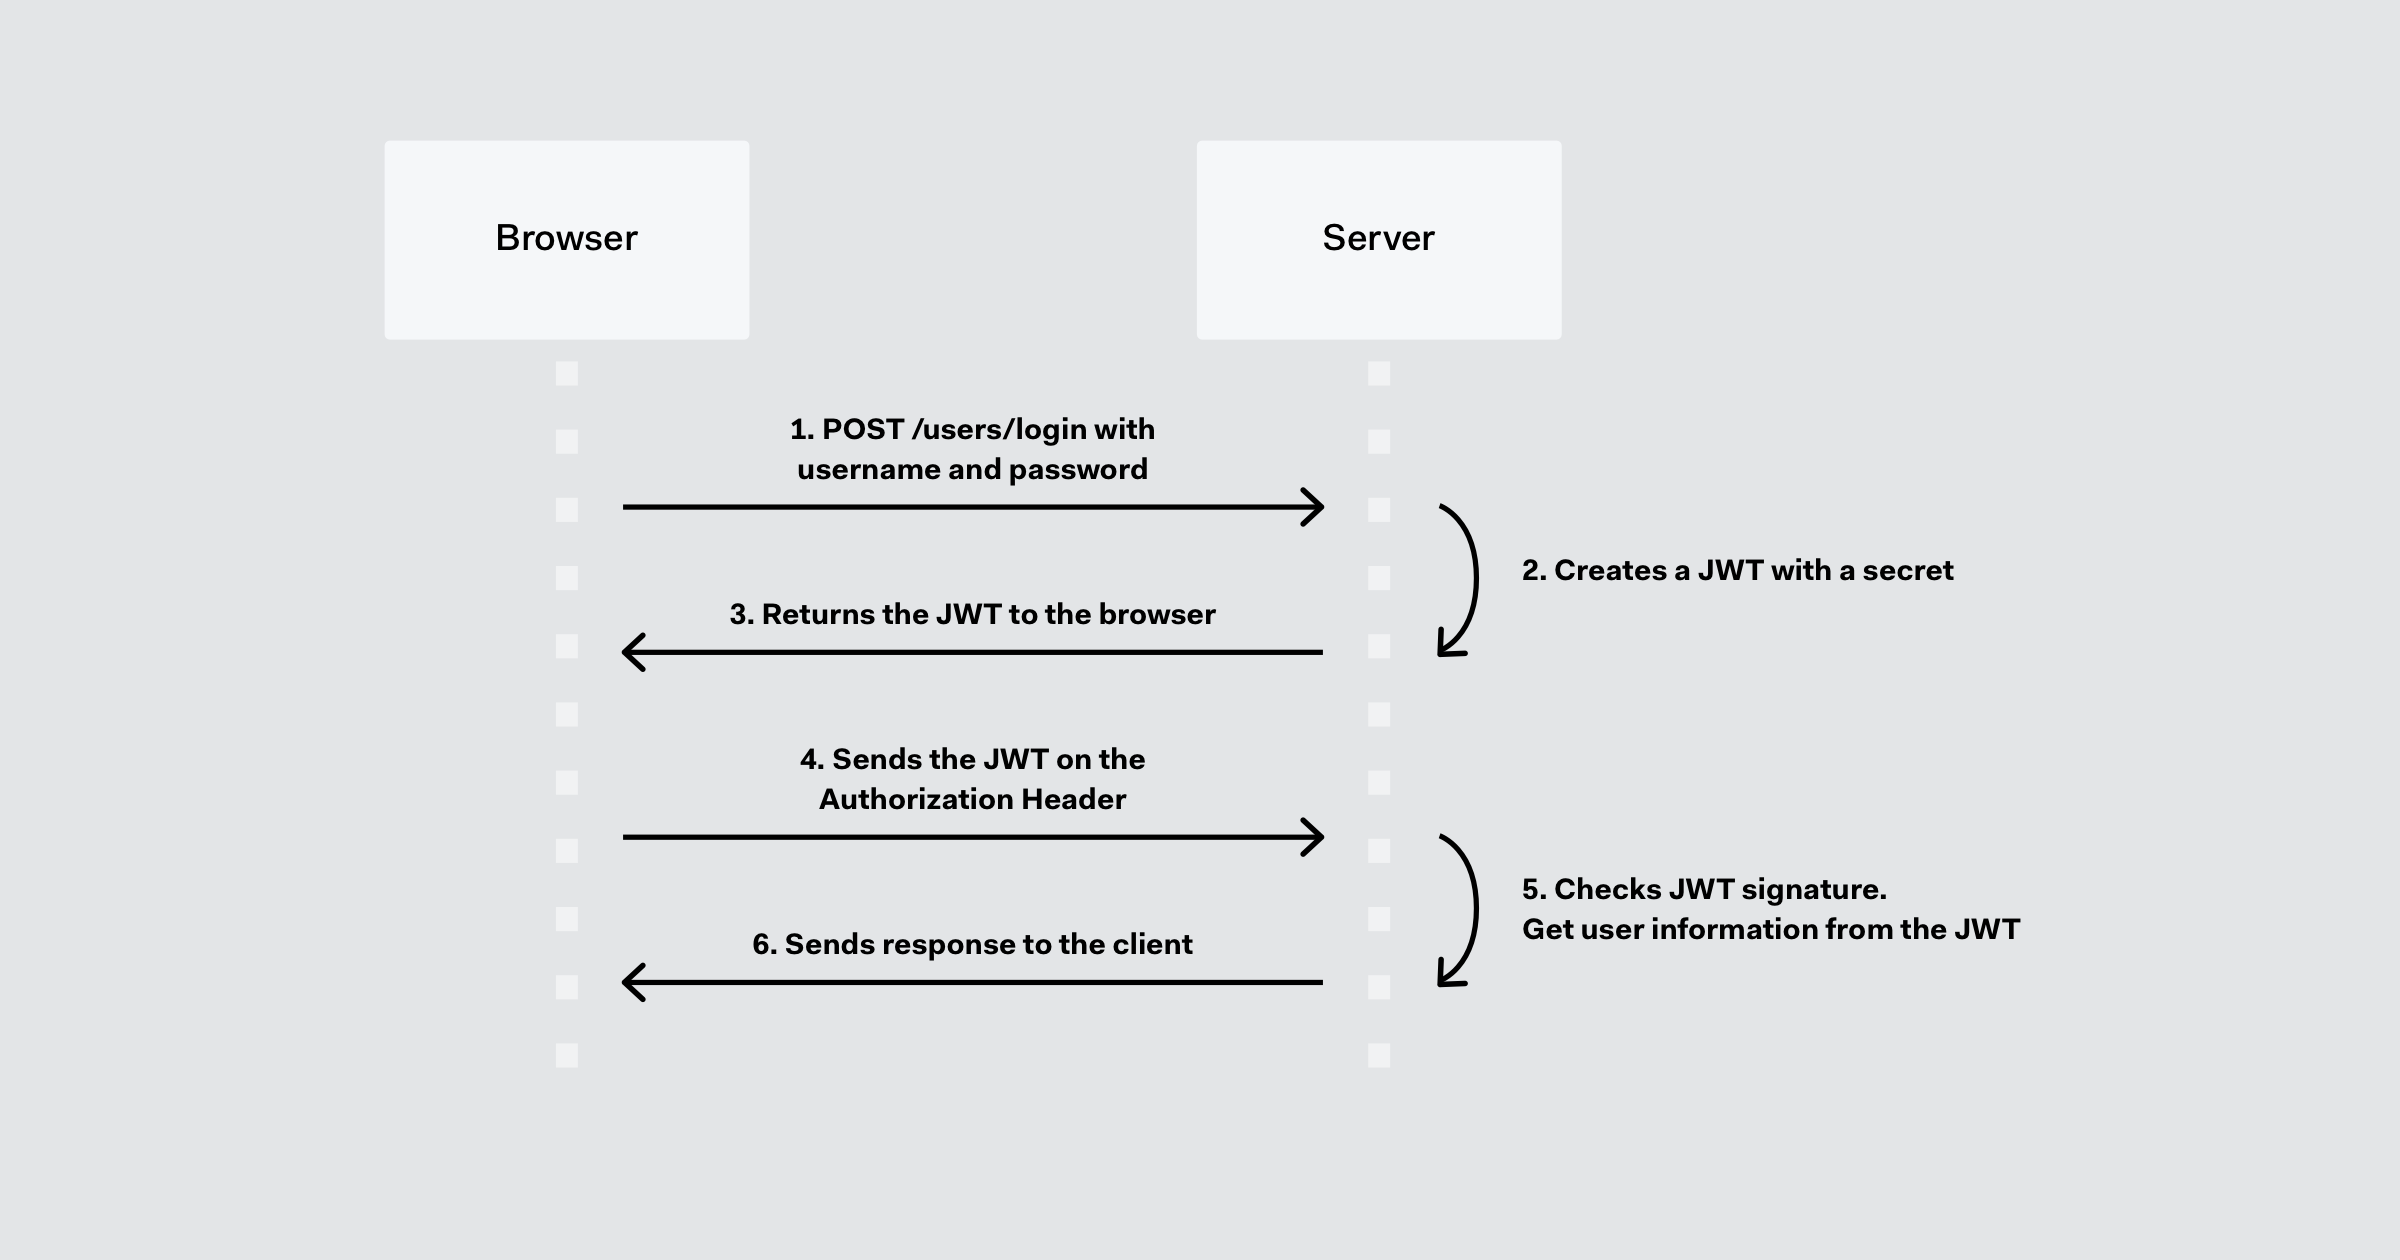
\includegraphics[width=1\textwidth,height=\textheight]{img/Schrempf/jwt-auth-process.png}
\caption{JWT Authentikationsablauf
{[}\protect\hyperlink{ref-jwt}{31}{]}}
\end{figure}

\hypertarget{continuous-integration-und-continuous-deployment}{%
\subsubsection{Continuous Integration und Continuous
Deployment}\label{continuous-integration-und-continuous-deployment}}

\begin{figure}
\centering
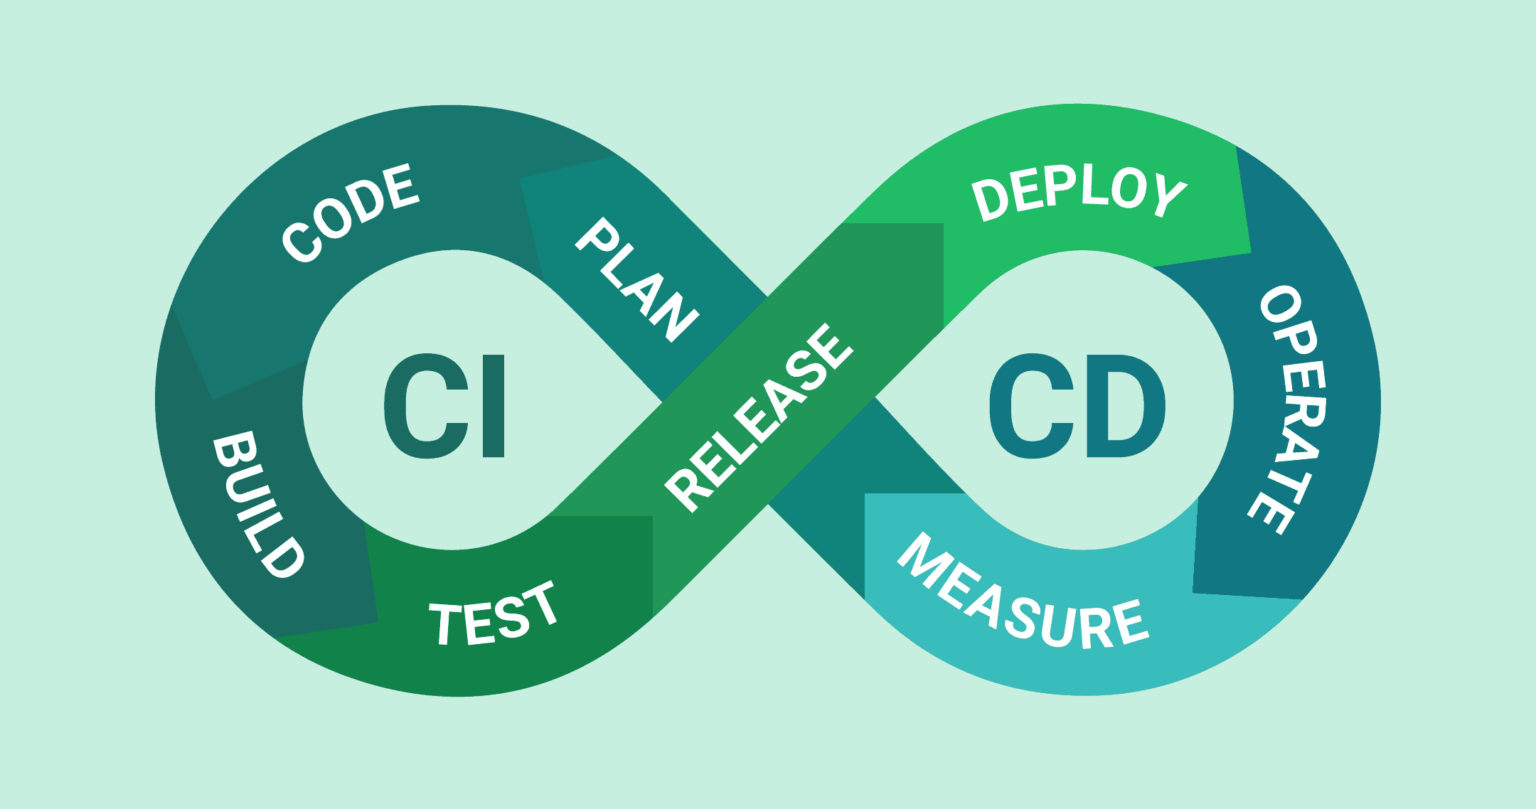
\includegraphics[width=1\textwidth,height=\textheight]{img/Schrempf/ci-cd.png}
\caption{CI / CD Ablauf {[}\protect\hyperlink{ref-bestarion}{33}{]}}
\end{figure}

CI / CD\footnote{Continuous Integration und Continuous Deployment} ist
ein Konzept, welches Entwicklerteams, dazu anregt, kontinuierlich und in
kürzeren Abständen Dinge am Code zu ändern, diesen zu verbessern und zu
automatisieren. Wie oben dargestellt, ist es ein nie endender Kreislauf.
Man unterscheidet zwei Komponenten voneinander: Die Continuous
integration und das Continuous delivery.

Unter CI\footnote{Continuous Integration} versteht man das tatsächliche
Entwickeln, Testen und Hochladen des Codes in das VCS\footnote{Version
  Control System}. Dies wird durch verschiedene Methoden und Prozesse
erleichtert, wie zum Beispiel automatisches Testen des Programms oder
agiles Projektmanagement.

Das Testen einer Applikation ist ein essenzieller Weg zum Erfolg. CI
befasst sich unter anderem mit den Wegen, wie ich mein Programm auf
besten Wege prüfen kann. Mit dieser Technologie wird der Grundstein für
unter anderem automatisches Unit-, Integration-, Regression-,
Performancetesten gelegt.

Unter CD\footnote{Continuous Deployment} versteht man das deployen von
Software auf verschiedene Umgebungen. Hier fallen, wie oben angedeutet,
Testumgebungen auch darunter, sowie Entwicklungsumgebungen und
Produktivsysteme. Dieser ganze Prozess ist im nun komplett automatisiert
und wird bei verschiedenen Events
getriggert.{[}\protect\hyperlink{ref-bestarion}{33}{]}

Um dieses sehr mächtige Konzept voll auszuschöpfen werden Pipelines
angelegt. Diese verrichten die Arbeit, welche ansonsten manuell
verrichtet werden müsste. Hier ein kleiner Ausblick:

\begin{enumerate}
\def\labelenumi{\arabic{enumi}.}
\tightlist
\item
  Definierte Tests aufsetzten und ausführen
\item
  Code packages erstellen
\item
  Verschiedene Umgebungen mittels Umgebungsvariablen vorbereiten
\item
  Code deployen
\item
  Versionen releasen
\end{enumerate}

\hypertarget{docker}{%
\paragraph{Docker}\label{docker}}

Um solch ein großes Konzept überhaupt realisieren zu können, muss man
sich ein Stück weit von der bisherigen Softwareentwicklung lossagen.
Hier kommen Microservices und die Containerization ins Spiel.

Microservices sind Teile eines Produkts. Früher gab es nur einen
einzigen großen Softwaremonolithen, welcher mit seinen Teilen als ein
großes Ganzes funktionierte. Heutzutage werden Teile identifiziert und
jeder Baustein wird für sich issoliert programmiert. Dies bietet mehrere
Vorteile. Bei einer konzeptionellen oder technischen Umstellung kann die
einzelne Komponente leicht ausgetauscht und durch eine neue ersetzt
werden. Außerdem ist die gesamte Software als auch einzelne Teile leicht
Skallierbar. Jedes einzelne Element läuft in seiner dezidierten
Umgebung, welche nur den Kernel mit dem OS\footnote{Operating System}
teilt und deswegen auch unabhängig auf verschiedenen Systemen
einsatzbereit ist. Solch ein dezidierte Umgebung besteht aus
Systembibliotheken, Abhängikeiten, Umgebungsvariablen und eventuellen
eigenproduzierten Code der zu hostenden Anwendung. Dies ist ein
Container. Es gilt: Funktioniert der Container, und somit auch der in
ihm definierte Microservice auf einem System, so tut er es auch überall
anders. Außerdem können Container auch leicht in Clouds deployd und
gehosted werden. Solch ein Aspekt ist vorallem in Zeiten immer stärker
werdenden Cloud-Computings immer wichtiger.
{[}\protect\hyperlink{ref-ibm-docker}{34}{]}

Ein Container benutzt die Virtualisierungstools des Linuxkernels um
Ressourcen zu teilen und verwalten. Für nicht Unix-Betriebsysteme gibt
es Software die den Linuxkernel simmulieren kann. Zum Beispiel
WSL\footnote{Windows-Subsystem für Linux} oder Hyper-V bei Windows.
Durch die gemeinsame Nutzung des Kernels muss auch keine dezidierte
Definition der benötigten Ressourcen stattfinden, da diese automatisch
vom System alloziert werden. Das Konzept eines Containers ähnelt dem,
einer VM\footnote{Virtuelle Maschine}. Nur mit dem wesentlichen Vorteil,
dass kein komplett eigenes OS verwendet wird, sondern nur die Schritte
zum produzieren eines gewissen Outputs angegeben werden. Container haben
eine Abstraktionsebene zum Kernel, aber da eben kein eigenes
Betriebsystem wie bei einer VM verwendet wird, gibt es auch ein
marginales Sicherheitsrisiko. Malware könnte durch die gemeinsame
Nutzung des Kernels eben auf diesen zugreifen und erheblichen Schaden
anrichten. Um dem Vorzubeugen, gibt es etliche Third-Party Tools mit
denene die Sicherheit über das schon gegebene Maß erhöht werden kann.
{[}\protect\hyperlink{ref-ibm-docker}{34}{]}

\begin{figure}
\centering
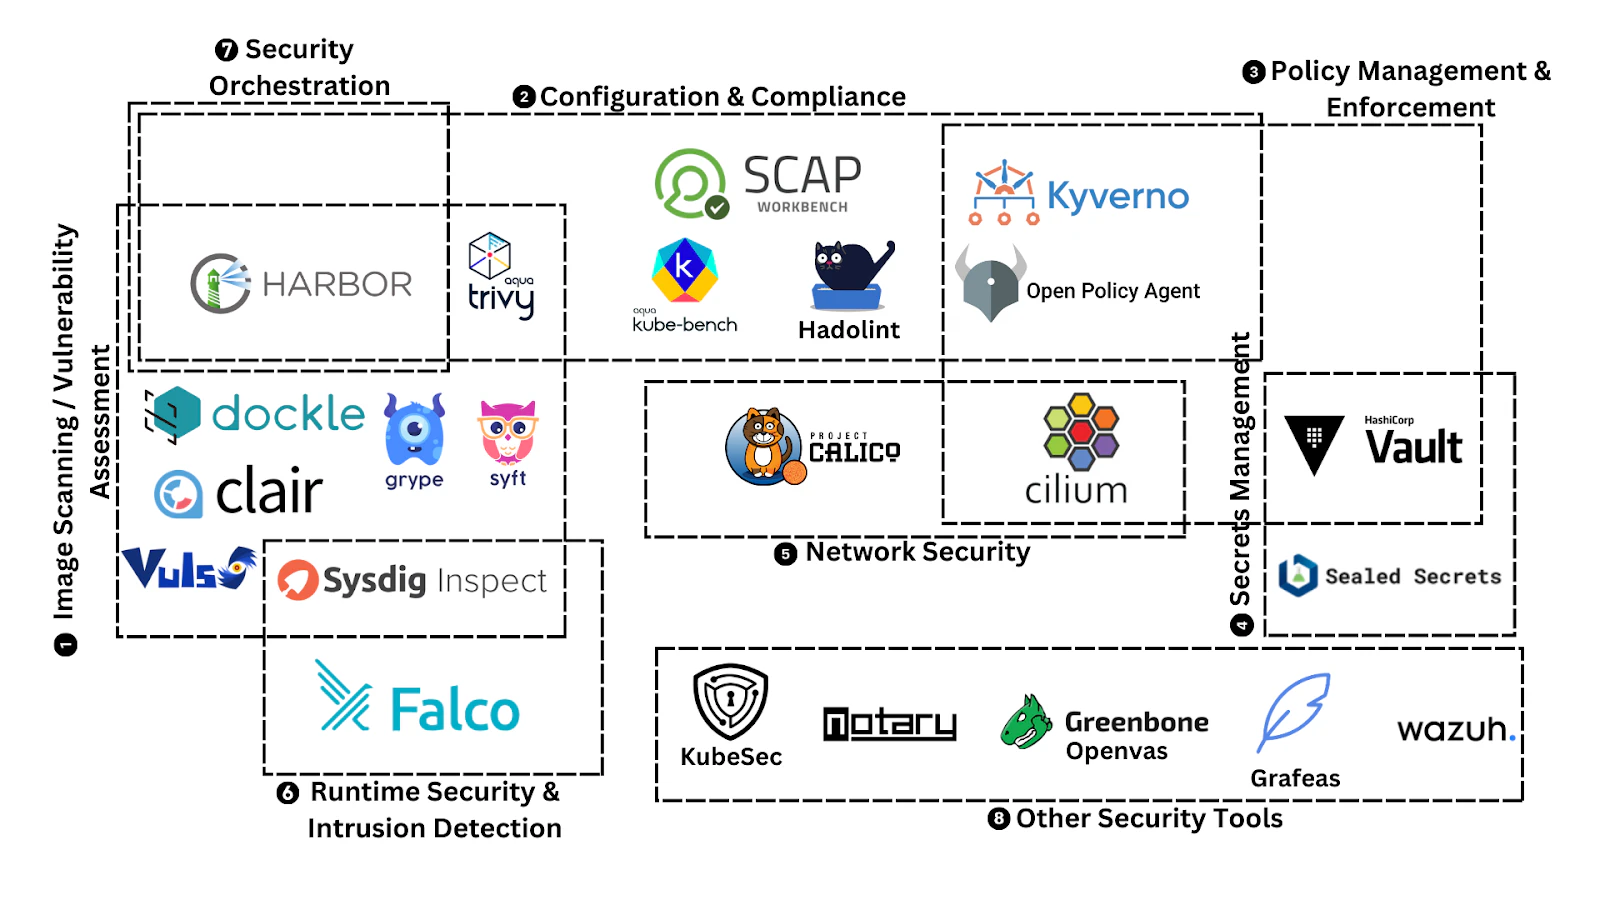
\includegraphics[width=1\textwidth,height=\textheight]{img/Schrempf/container-security-tools.png}
\caption{Übersicht von Container Security Tools
{[}\protect\hyperlink{ref-docker-security}{35}{]}}
\end{figure}

Soweit zum Allgemeinen der Virtualisierung. Doch was hat Docker damit zu
tun? Docker ist ein Open Source Projekt, welches sich auf die
Containerization spezialisiert hat. Es bietet einen riesigen freien
Markt (Docker Hub) zur Erstellung und Distribution von Docker Images an.
Es wird so verwaltet, dass es verschiedene Registries gibt. Pro Registry
gibt es die verschiedenen Versionen eines Images. Ein Registry wird mit
username/image-name benannt. Ein Image ist das zuvor genannte Äquivalent
zu der Definition eines Containers. Ein Image ist in Schichten aufgebaut
und jede Schicht stellt einen neuen Zustand des Containers dar. Das
vollständig ausgeführte und unter Umständen auch angepasste Image ist
dann der laufende Container. Auf Basis eines Images können mehrere
Container laufen. {[}\protect\hyperlink{ref-ibm-docker}{34}{]} Jedes
Image hat einen Entrypoint. In diesem wird spezifiziert, was geschehen
soll, wenn der Container (zum ersten mal) gestartet wird.

Jedes Image wird in einem \passthrough{\lstinline!Dockerfile!}
definiert. Hierbei spricht man nur von einer Datei, in welcher die
Anweisungen zum Aufbau der Schichten gespeichert sind. Beim Starten des
Containers interagiert die Docker CLI\footnote{command line interface}
mit dem \passthrough{\lstinline!Dockerfile!} und führt die Anweisungen
aus. Eine beliebte Variante ist es, ein schon bestehendes Image zu
verwenden und seine eigene Applikation mit Schichten on top zu bauen.
{[}\protect\hyperlink{ref-ibm-docker}{34}{]}

Ein \passthrough{\lstinline!Dockerfile!} ist sehr vielseitig und bietet
verschiedene Funktionen. Eine sehr wichtige sind Secrets. Diese stehen
für Platzhalter, in die der Anwender Werte eingibt, welche im weiteren
Programmablauf benötigt werden. Oftmals werden sie als
Umgebungsvariablen realisiert. Eine wichtige Eigenschaft solch einer
Einheit ist, dass es ein eigenes System ist, welches unabhängig vom Host
existiert. Dementsprechend gehen im Container gespeicherte Daten und
Änderungen verloren, wenn dieser heruntergefahren wird. Um dieses
Problem zu beheben, gibt es Volumes. Sie dienen dazu, Daten in den
Container, z.B. Code, und aus ihm heraus, z.B. Datenbanken, zu bekommen.
Um aus dem Container heraus kommunizieren zu können, muss ein
Portforwarding zwischen Host und Cotnainer eingestellt werden.

\begin{figure}
\centering
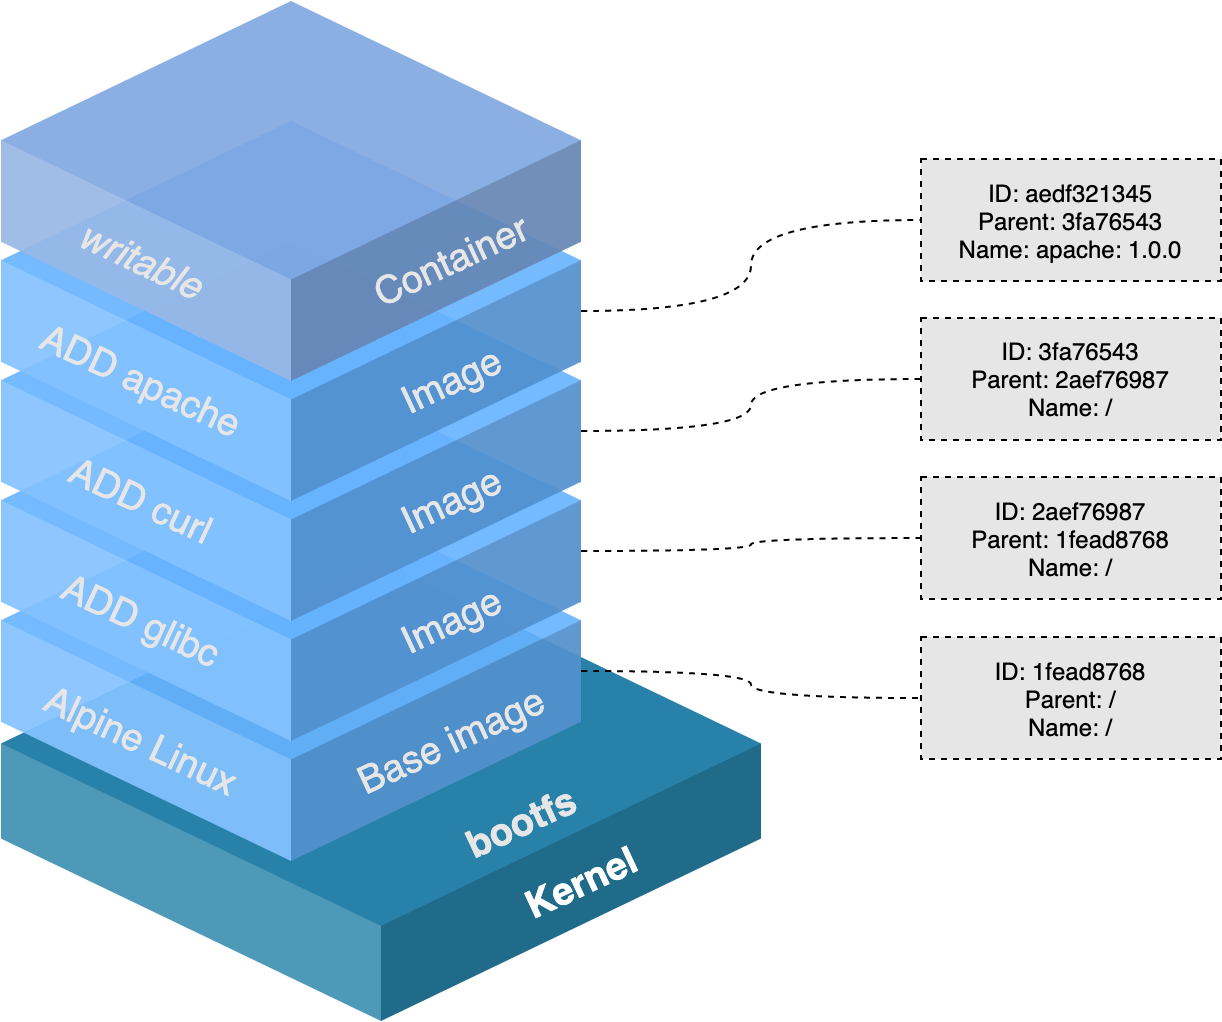
\includegraphics[width=0.8\textwidth,height=\textheight]{img/Schrempf/container-layers-overview.png}
\caption{Containerschichten
{[}\protect\hyperlink{ref-docker-image-layers}{36}{]}}
\end{figure}

\begin{figure}
\centering
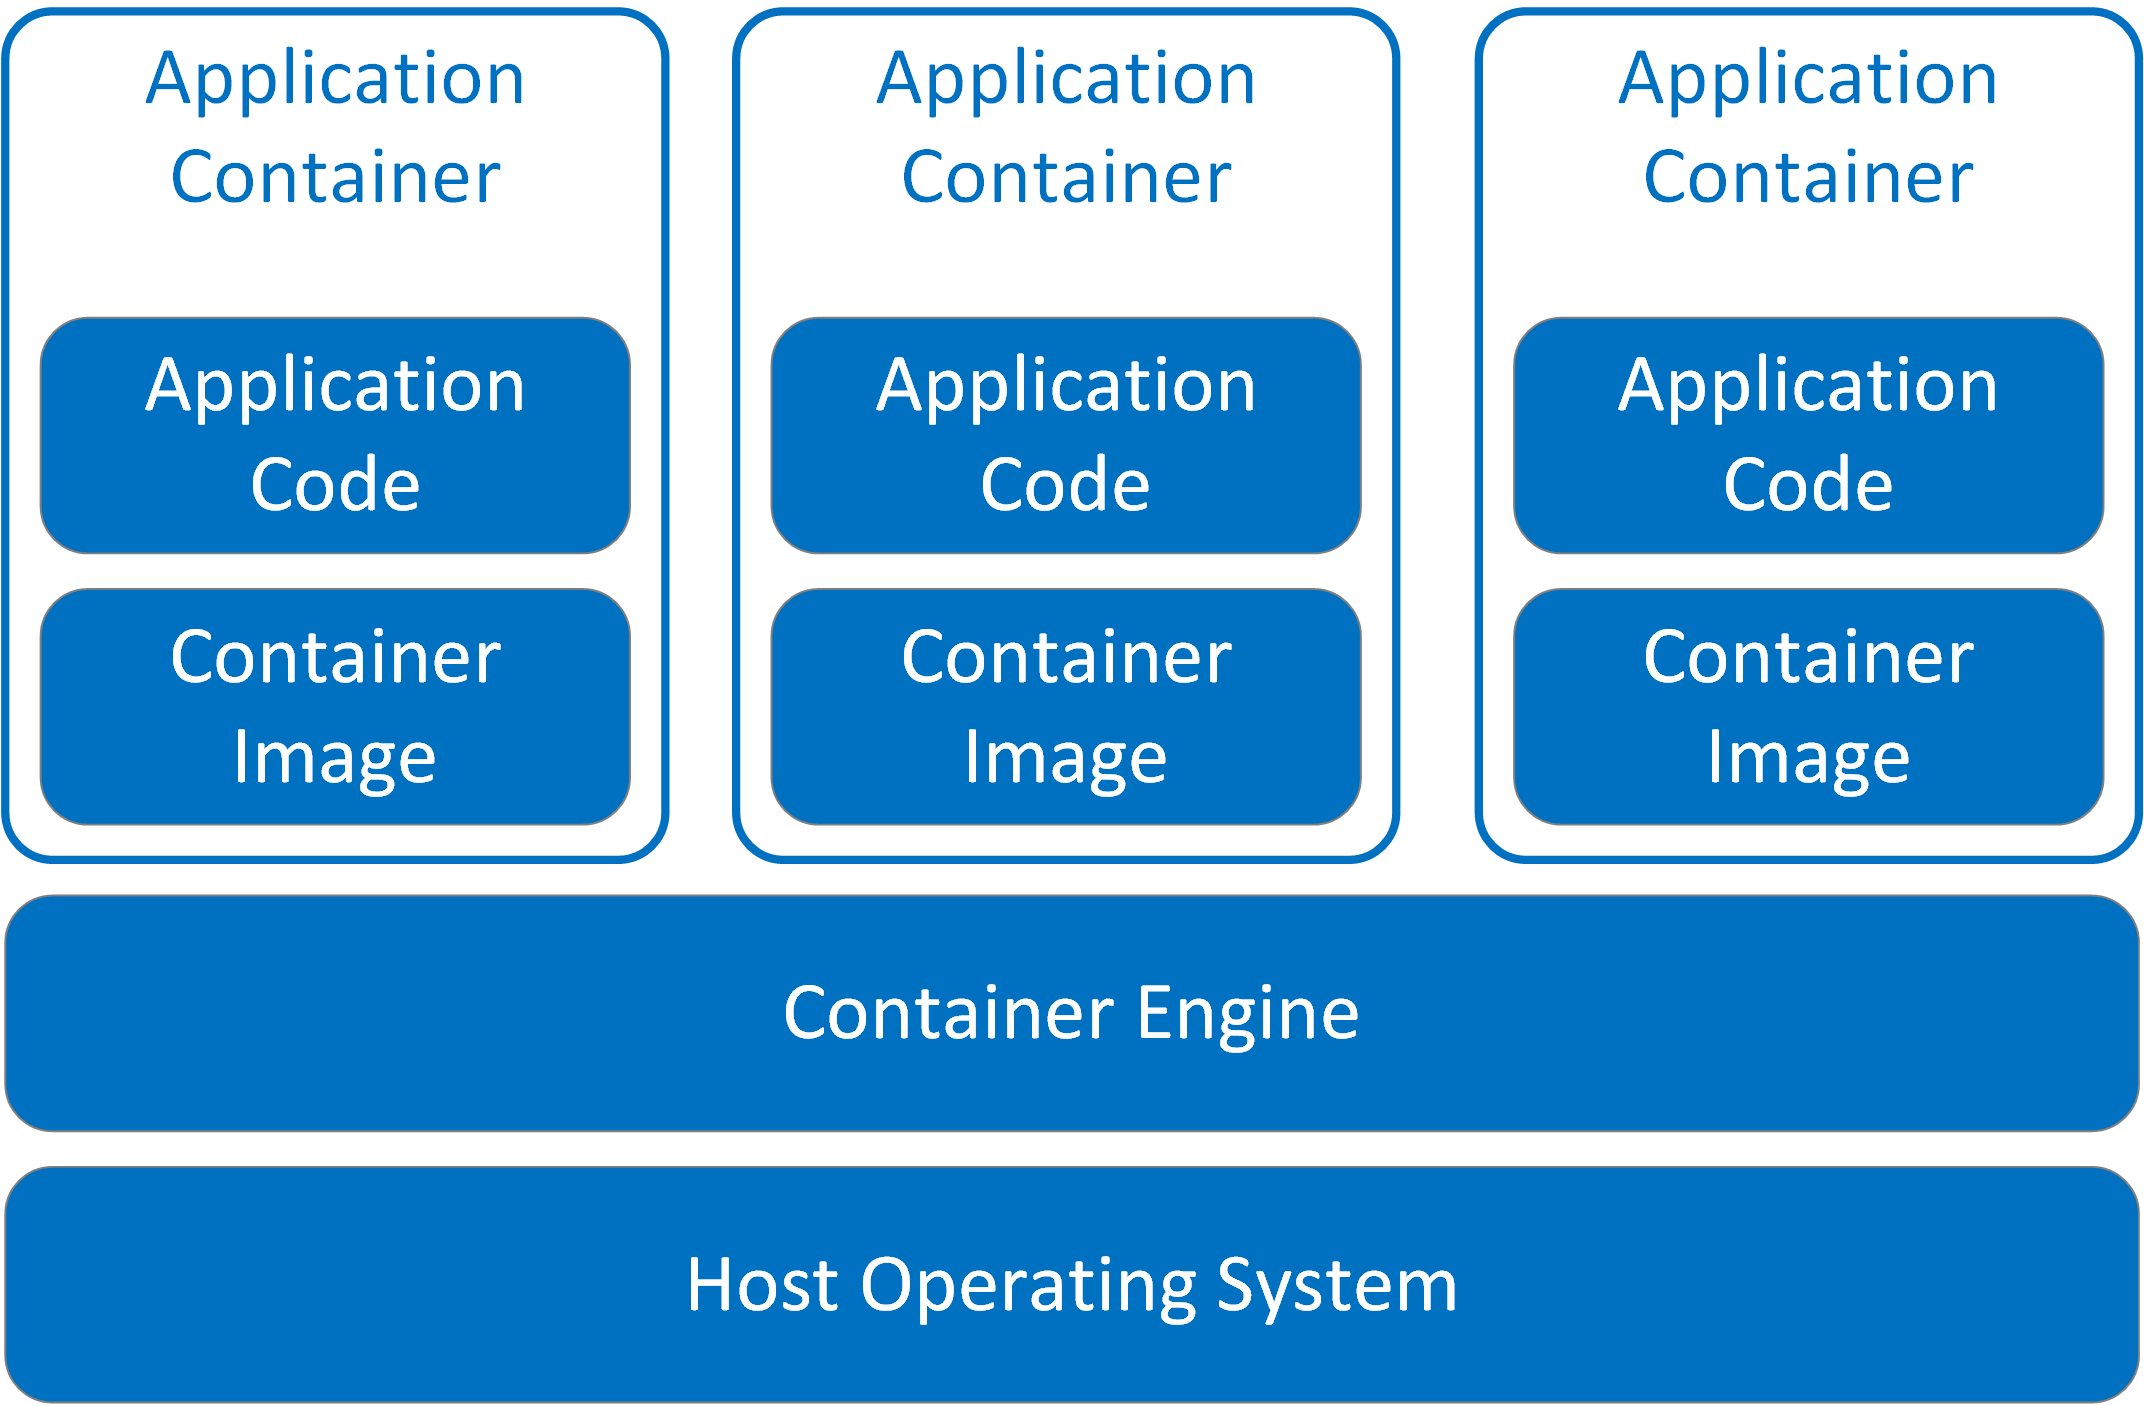
\includegraphics[width=0.8\textwidth,height=\textheight]{img/Schrempf/container-infrastructure-overview.png}
\caption{Übersicht vom Containeraufbau
{[}\protect\hyperlink{ref-container-overview}{37}{]}}
\end{figure}

Ein Beispiel solch eines Dockerfiles ist hier zu sehen. Es baut auf das
schon bestehenden Ubuntu-Image auf, installiert Python, fügt eine Datei
hinzu, schaltet die benötigten Ports frei und führt das Python-Script
aus. {[}\protect\hyperlink{ref-docker-dockerfile}{38}{]}

\begin{lstlisting}[caption={Beispiel eines Dockerfiles}]
# syntax=docker/dockerfile:1
FROM ubuntu:22.04

# install app dependencies
RUN apt-get update && apt-get install -y python3 python3-pip
RUN pip install flask==3.0.*

# install app
COPY hello.py /

# final configuration
ENV FLASK_APP=hello
EXPOSE 8000
CMD ["flask", "run", "--host", "0.0.0.0", "--port", "8000"]
\end{lstlisting}

{[}\protect\hyperlink{ref-docker-dockerfile}{38}{]}

Docker compose ist eine Funktionalität von Docker. Es ermöglicht die
Definition von mehreren Microservices in einer
YAML\footnote{yet another markup language}-Konfigurationsdatei Namens
\passthrough{\lstinline!compose.yml!}. Hier wird ein Microservice nur
Service genannt. Ein Service kann wieder als Dockerfile definiert werden
oder sogar das Image vom Docker Hub benutzt und in der Datei bis zu
einem gewissen Maß weiter spezialisiert werden. In der
\passthrough{\lstinline!compose.yml!} werden Ports, Secrets, zu
benutzende Volumes, Networks und die Anzahl der Container des Services
beschrieben. Da nun mehrere Microservices zwar als Bausteine definiert
werden, jedoch miteinander interagierene können um ein ganzes Konstrukt
zu bilden, gibt es die sogenanten Networks. Über diese können Tasks, wie
Containerübergreifende Datenkommunikation, realisiert werden. So sieht
eine \passthrough{\lstinline!compose.yml!} Datei grundelegend aus:
{[}\protect\hyperlink{ref-docker-compose}{39}{]}

\begin{lstlisting}[caption={Beispiel eines docker compose files}]
services:
  frontend:
    image: example/webapp
    ports:
      - "443:8043"
    networks:
      - front-tier
      - back-tier
    configs:
      - httpd-config
    secrets:
      - server-certificate

  backend:
    image: example/database
    volumes:
      - db-data:/etc/data
    networks:
      - back-tier

volumes:
  db-data:
    driver: flocker
    driver_opts:
      size: "10GiB"

configs:
  httpd-config:
    external: true

secrets:
  server-certificate:
    external: true

networks:
  front-tier: {}
  back-tier: {}
\end{lstlisting}

Ein weitere Funktionalität von Docker ist Docker Swarm. Mit diesem Tool
wird eine Orchestrierungsmöglichkeit für Anwendungen mit mehr als einem
Host angeboten. Hierbei kann man die Anzahl der Container per Host
angeben, wo welcher Container laufen soll und vieles mehr. Beschrieben
wird das Verhalten des Swarms über eine leicht anders funktionierende
Version der \passthrough{\lstinline!compose.yml!}. Jedoch ist
anzumerken, dass Docker Swarm nicht so ausgereift und mehr so etwas in
der Art wie ein Notbehelf aufgrund der Nachfrage ist. Für kontrollierte
und ausführliche Ochestrierung wird ein explizit dafür ausgelegtes
Framework, wie Kubernetes, empfohlen.
{[}\protect\hyperlink{ref-docker-swarm}{40}{]}
{[}\protect\hyperlink{ref-circleci-blog}{41}{]}

\hypertarget{pipeline}{%
\paragraph{Pipeline}\label{pipeline}}

Wie oben angedeuted, nehmen Pipelines dem Programmierer sehr viel arbeit
ab. Verschiedene Plattformen haben verschiedene Möglichkeiten Pipelines
zu benutzen, definieren und auszuführen. Beispiele wären Jenkins oder so
wie es in dieser Ausarbeitung verwendet worden ist: GitHub. GitHub
bietet GitHub Actions an. Hierbei schreibt man eine YAML-Datei in der
steht, was wann wie geschehen soll und legt sie im Verzeichnis
\passthrough{\lstinline!.github/workflows!} in seinem Repository ab.
Wenn die Action ausgelöst wird, startet GitHub eine VM mit dem unter dem
Tag \passthrough{\lstinline!runs-on!} definierten Betriebsystem, welche
die weiteren definierten Tasks ausführt.

Eine GitHub Action besteht aus folgenden Komponenten:

\begin{enumerate}
\def\labelenumi{\arabic{enumi}.}
\tightlist
\item
  Event

  \begin{itemize}
  \tightlist
  \item
    Trigger für Workflow
  \end{itemize}
\item
  Runner

  \begin{itemize}
  \tightlist
  \item
    Runtime Environment z.B. Ubuntu
  \end{itemize}
\item
  Job(s)

  \begin{itemize}
  \tightlist
  \item
    Die durch das Event getriggerten Workflows
  \end{itemize}
\item
  Steps

  \begin{itemize}
  \tightlist
  \item
    Ein Workflow hat mehrere Steps
  \end{itemize}
\item
  Action

  \begin{itemize}
  \tightlist
  \item
    Ein Step hat mehrere Actions
  \item
    Was in diesen Step ausgeführt wird
  \end{itemize}
\end{enumerate}

Hier wird eine workflow.yml dargestellt, welche eine Java-Applikation
beim Push-Event testet.

\begin{lstlisting}[caption={Beispiel einer GitHub Action}]
name: Test

on:
  push:

permissions:
  contents: read
  actions: read

jobs:
  test:
    runs-on: ubuntu-latest

    steps:
      - name: Checkout code
        uses: actions/checkout@v4

      - name: Set up JDK 21
        uses: actions/setup-java@v4
        with:
          java-version: '21'
          distribution: 'temurin'
          cache: maven

      - name: Run Tests
        run: mvn clean test
\end{lstlisting}

Weitere mögliche automatisierte Anwengungsfälle sind:

\begin{itemize}
\tightlist
\item
  Einen Release bei Softwareänderungen erstellen

  \begin{itemize}
  \tightlist
  \item
    Eine App auf dem Google / Apple Store hochladen
  \end{itemize}
\item
  Den geänderten Code auf dem Produktivsystem updaten

  \begin{itemize}
  \tightlist
  \item
    Docker Images updaten und hochladen
  \item
    Pullen der neuen Images auf dem Server
  \end{itemize}
\end{itemize}

\hypertarget{rest-api}{%
\subsubsection{REST API}\label{rest-api}}

Eine API\footnote{Application Programming Interface} ist
Programmierschnittstelle, die dafür entworfen worden ist, um autonomen
Anwendungen das Kommunizieren und den Austausch von Daten zu erleichtern
und zwischen ihnen zu standardisieren. REST\footnote{Representational
  State Transfer} ist ein Prinzip, welches verschieden umgesetzt werden
kann, als Zwischendienst zwischen dem Client und dem Backend dient und
als Schnitstelle zum Abrufen von Ressourcen vom Client and den Server
verwendet wird. Hierbei nutzt man URIs\footnote{Uniform Resource
  Identifier}. Ein Uniform Resource Identifier ist dafür da, eine
Ressource eindeutig zu identifizieren.
{[}\protect\hyperlink{ref-REST-API-Design-Rulebook}{42}{]}

Bei RESTful APIs sendet der Client eine Anfrage über HTTP\footnote{Hypertext
  Transfer Protocol} an eine URI und bekommt daraufhin seine Antwort.
{[}\protect\hyperlink{ref-redhat-rest}{43}{]} Die möglichen Anfragearten
des Clients nennt man HTTP-Methodes und diese sind:
{[}\protect\hyperlink{ref-mozilla-rest}{44}{]}

\begin{itemize}
\tightlist
\item
  GET

  \begin{itemize}
  \tightlist
  \item
    Ruft eine Ressource vom Server ab, ohne den Zustand der Ressource zu
    verändern.
  \end{itemize}
\item
  HEAD

  \begin{itemize}
  \tightlist
  \item
    Ruft nur die Header-Informationen einer Ressource ab, ohne den
    eigentlichen Inhalt.
  \end{itemize}
\item
  POST

  \begin{itemize}
  \tightlist
  \item
    Sendet Daten an den Server, um eine neue Ressource zu erstellen.
  \end{itemize}
\item
  PUT

  \begin{itemize}
  \tightlist
  \item
    Erstellt eine neue Ressource oder aktualisiert eine bestehende
    vollständig.
  \end{itemize}
\item
  DELETE

  \begin{itemize}
  \tightlist
  \item
    Löscht eine Ressource auf dem Server.
  \end{itemize}
\item
  OPTIONS

  \begin{itemize}
  \tightlist
  \item
    Ruft Informationen über die Kommunikationsoptionen mit dem Server
    ab.
  \item
    Gibt zurück, welche HTTP-Methoden und Header von einer URI
    unterstützt werden.
  \end{itemize}
\item
  TRACE

  \begin{itemize}
  \tightlist
  \item
    Gibt die Anfrage so zurück, wie sie der Server erhalten hat.
  \end{itemize}
\item
  PATCH

  \begin{itemize}
  \tightlist
  \item
    Aktualisiert eine Ressource teilweise, ohne sie vollständig zu
    ersetzen.
  \end{itemize}
\end{itemize}

\hypertarget{design}{%
\paragraph{Design}\label{design}}

Es gibt zwar verschiedene Ansätze so eine API umzusetzen, jedoch gibt es
Richtlinien und Best-Practices. Die Antwort des Servers and den Client
sollte in JSON verfasst sein. Um die Skalierbarkeit der Anwendungen zu
garantieren, ist eine Server nicht dazu verpflichtet, den Status einer
Ressource sich zu merken. Diese Aufgabe obligt rein dem Client.
{[}\protect\hyperlink{ref-REST-API-Design-Rulebook}{42}{]}

Eine URI soll klar verständlich und strukturell aufklärend designed
sein. Wenn man die URI begutachtet, soll genau ersichtlich sein, welche
Ressource man bei Aufruf erhält. Der Aufbau ist in der RFC 3986
beschrieben unter dem Format:

\passthrough{\lstinline!URI = scheme "://" authority "/" path [ "?" query ] [ "\#" fragment ]!}

\textbf{URI Namensregeln}:

\begin{itemize}
\tightlist
\item
  Ein / wird für hierachische Abhängikeiten benutzt

  \begin{itemize}
  \tightlist
  \item
    Ein / darf nicht am Ende einer URI stehen, da es sonst zu Verwirrung
    führen kann, ob eine neue Ressource anfängt oder nicht
  \end{itemize}
\item
  Zusammengesetzte Wörter sind mittels - zu trennen

  \begin{itemize}
  \tightlist
  \item
    Ein \_ als Trennzeichen ist aufgrund der erschwerte Lesbarkeit zu
    vermeiden
  \end{itemize}
\item
  Groß- und Kleinschreibung

  \begin{itemize}
  \tightlist
  \item
    In Schema und Authority wird sie ignoriert
  \item
    Im Path wird sie berücksichtigt
  \item
    Um unnötige Probleme zu vermeiden soll die gesamte URI klein
    geschrieben werden
  \end{itemize}
\item
  File extensions dürfen nicht in in der URI vorkommen
\item
  Widerspruchsfreie Namen für Subdomains.
\item
  CRUD\footnote{Create, Read, Update, Delete} Namen dürfen in keinem
  Part der URI verwendet werden.
  {[}\protect\hyperlink{ref-REST-API-Design-Rulebook}{42}{]}
\end{itemize}

\textbf{URI Designregeln}:

\begin{itemize}
\tightlist
\item
  Jeder neue / bedeutet einen neuen Path und somit eine neue abfragbare
  Ressource.

  \begin{itemize}
  \tightlist
  \item
    Jeder einzelne Path beinhaltet eine abfragbare Ressource.
  \item
    Paths sind mit Nomen zu benennen.
  \item
    Paths bei denen nur ein Datenpunkt übermittelt wird, sind im
    Singular zu benennen.

    \begin{itemize}
    \tightlist
    \item
      Solche Paths werden Document genannt
    \end{itemize}
  \item
    Paths bei denen ein Set an Daten zurückgegeben wird, sind im Plural
    zu benennen.

    \begin{itemize}
    \tightlist
    \item
      Solche Paths werden Collection genannt
    \end{itemize}
  \end{itemize}
\item
  Stores sind Path Variables und können anstelle eines Nomens eingesetzt
  werden.

  \begin{itemize}
  \tightlist
  \item
    Ein Store erzeugt keine neue URI.
  \item
    Ein Store benennt eine Ressource in der URI.
  \item
    Ein Store wird zur genauerene Identifikation / Spezifikation einer
    Ressource verwendet. (z.B. ID)
  \end{itemize}
\item
  Controller Elemente werden als letztes and die URI angehängt.

  \begin{itemize}
  \tightlist
  \item
    Sie können nicht den CRUD-Operationen zugeordnet werden.
  \item
    Sie spiegeln aufrufbare Funktionen wider.
  \item
    Verben sind für die Namensgebung zu verwenden.
  \end{itemize}
\item
  Eine URI soll im Schema
  \passthrough{\lstinline!\{collection\}/\{store\}/\{document\}!}
  aufgebaut sein.
  {[}\protect\hyperlink{ref-REST-API-Design-Rulebook}{42}{]}
\end{itemize}

\textbf{URI Optionals}:

\begin{itemize}
\tightlist
\item
  Queries dienen dazu, Daten anzugeben, die nicht strikt aneinander
  gekoppelt sind, jedoch miteinander korrelieren.

  \begin{itemize}
  \tightlist
  \item
    Der Inhalt der Base-URI darf sich nicht durch das Weglassen eines
    Query-Parameters verändern.
  \item
    Sie werden auf Collections und Stores angewandt.
  \item
    Sie dienen meistens zum Suchen / Filtern der Daten aus einer
    Ressource.
    {[}\protect\hyperlink{ref-REST-API-Design-Rulebook}{42}{]}
  \end{itemize}
\item
  Fragemnts werden nach Queries angegeben und geben eine spezifische
  Sektion oder ein Element in der URI an.

  \begin{itemize}
  \tightlist
  \item
    Sie sind bei der Navigation auf der Webpage hilfreichn
  \item
    Sie können die Status einer Webpage angeben / ändern ohne diese neu
    laden zu müssen.
    {[}\protect\hyperlink{ref-medium-uri-fragment}{45}{]}
  \end{itemize}
\end{itemize}

Beispiele von URIs nach besprochenem Konzepten sind
\passthrough{\lstinline!https://api.contrude.eu/sensors/42/7/temperature?latest=true!}
oder
\passthrough{\lstinline!https://contrude.eu/ships?user=123\#page2!}.

\hypertarget{javascript}{%
\paragraph{JavaScript}\label{javascript}}

Mit Frameworks wie Node.js kann auch eine frontendorientierte Sprache
wie JavaScript fürs Backend genutzt werden. Ein großer Vorteil von
Node.js, welcher es auch attraktiv für API-Design macht, ist seine
ereignisgesteuerte, nicht-blockierende Umsetzung. Dieses mächtige
Framework bietet sehr viele Packages an, was auch die Entwicklung sehr
modular gestaltet. Express ist ein Modul, welches den Prozess des API
Programmierens erleichtert. Anzumerken ist jedoch, dass Express keine
wirkliche Funktionalität für REST-Services anbietet, sondern nur das
Erstellen von Routes (path + query + fragment) ermöglicht. In die Routes
muss man die selbst progammierte Middleware einbinden, welche dann als
Backend fungiert, weitere Funktionen aufruft, Prozesse startet oder
direkt mit Datenbanken kommuniziert.

Um eine Node.js REST-Appp zu erstellen, muss man als erstes einen Ordner
seiner Wahl als ein Node.js project initialisieren. Als Package-Manager
wird hier NPM verwendet.

\begin{lstlisting}[caption={Initialisieren eines Node.js Projekts}]
  npm init
\end{lstlisting}

Danach können benötigte Packages installiert werden. In unserem fall
Express.

\begin{lstlisting}[caption={Installieren vom Express package}]
npm install express
\end{lstlisting}

Eine JS Datei mit folgendem Inhalt muss noch erstellt werden um einen
REST-Express Server in der Node.js Anwendung zu starten:

\begin{lstlisting}[caption={Beispiel für eine REST Schnitstelle in Node.js}]
import express from "express";

const app = express(); // lässt die App Express verwenden
const port = 80; // Port, auf dem der Server läuft

// Middleware
app.use(express.json());

// API-Routen
// Route, um eine JSON-Antwort bei einer GET-Anfrage an /hello zu senden
app.get("/hello", (req, res) => {
  res.status(200).json({ message: "Hello Express" });
});

// Starte den Server auf zuvor definiertem Port
app.listen(port, () => {
  console.log(`Server läuft auf Port ${port}`);
});
\end{lstlisting}

Mit dem letzten Befehl

\begin{lstlisting}[caption={Starten einer Node.js Applikation}]
node app.js
\end{lstlisting}

wird die Applikation gestarted und kann auf
\passthrough{\lstinline!http://localhost:80/hello!} oder mittels cURL
und \passthrough{\lstinline!curl localhost/hello!} aufgerufen werden.
{[}\protect\hyperlink{ref-medium-rest-api}{46}{]}

Das JSON, welches beim aufrufen des Endpoints ausgegeben wird, sieht so
aus:

\begin{lstlisting}[caption={Ausgabe eines Beispiel-REST-Endpoints}]
{
  "message": "Hello Express"
}
\end{lstlisting}

\hypertarget{praktische-arbeit-1}{%
\subsection{Praktische Arbeit}\label{praktische-arbeit-1}}

\hypertarget{datenspeicherung-und-visualisierung-1}{%
\subsubsection{Datenspeicherung und
Visualisierung}\label{datenspeicherung-und-visualisierung-1}}

\hypertarget{mysql}{%
\paragraph{MySQL}\label{mysql}}

MySQL ist ein Open-Source RDBMS, welches von Oracle verwaltet wird.
Diese DB wird stetig weiterentwickelt und ist sogar optimal in der Cloud
hostbar. {[}\protect\hyperlink{ref-talend-mysql}{47}{]}

MySQL verwendet zwar keine Schemas wie andere DBMS, trotzdem kann man
mehrere Datenbanken innerhalb einer MySQL Instanz erstellen und somit
dieses Verhalten simulieren. Irreführend ist hierbei, dass man trotzdem
eine \textbf{DATABASE} und \textbf{SCHEMA} erstellen kann, obwohl sie
gleich behandelt werden. {[}\protect\hyperlink{ref-mysql-glosar}{48}{]}
Um möglichst lange Support-Updates mittels LTS\footnote{Long Term
  Support} Versionen zu erhalten, wurde hier die MySQL 8 Version
verwendet, obwohl sie offiziell noch nicht fertig ausprogrammiert ist.
{[}\protect\hyperlink{ref-mysql-lts}{49}{]}

Um die in diesem Projekt verwendeten Datenbanken zu erstellen, wurden
SQL-init-scripts geschrieben, welche die MySQL Instanz mit den
notwendigen Tabellen initialisieren, User anlegen und Dummy Daten
einfügen. Hierbei ist der Aufbau immer der gleiche:

\dirtree{%
.1 scripts.
.2 CreateDB.sql.
.2 CreateUser.sql.
.2 GrantPriveleges.sql.
.2 InsertDummyData.sql.
}

In \passthrough{\lstinline!CreateDB.sql!} ist die gesamte Struktur
mitsamt \textbf{DATABASE} und \textbf{SCHEMA} Erstellung geregelt.
Anzumerken ist hier, dass \textbf{CHECK} Constraints schon in vorherigen
Versionen semantisch akzeptiert, jedoch erst ab Version 8.0.16
tatsächlich umgesetzt wurden.
{[}\protect\hyperlink{ref-mysql-8.0.16}{50}{]} Aufgrund dessen, und des
später erklärten Microservice-Ansatzes, wurde für das gesamte Projekt
die Verison 8.0.29 verwendet. Da eine Datenbank ohne Daten nur halb so
viel wert ist und bei jeder einzelnen DB-Erstellung die Daten neu
einzugeben sehr mühsälig werden kann, gibt es die
\passthrough{\lstinline!InsertDummyData.sql!} Datei, in der die
Probedaten in die DB eingfügt werden.

In \passthrough{\lstinline!CreateUser.sql!} werden die Benutzer samt
ihrer Benutzergruppen und Berechtigungen erstellt. Diese Datei wurde für
jede DB verwendet, da sich kein Sinn für eine Änderung der Benutzer
ergab. Um den Code sicher pushen zu können, wurde ein vordefiniertes
Einmapasswort für jeden Datenbankbenutzer festgelegt, welches beim
ersten Login geändert werden muss. Zusätzlich wurde die Beschränkung
eingeführt, dass das geänderte Passwort nicht gleich den letzten fünf
sein darf. Zusätzlich darf jeder Benutzer, außer der API Benutzer, nur
maximal 4 aktive Datenbankconnections gleichzeitig haben. Eingestellt
wurde auch, dass eine SSL Zertifizierung, um die Sicherheit zu
gewährleisten, von jedem DB-User beim Anmelden anzugeben ist. Dieses
kann in den MySQL-Server eingespielt werden, wird aber auch automatisch
bei Initialstart der DB generiert. Ein User wird mit `name'@`bereich'
erstellt. Wobei der Bereich der Gültigkeitsbereich des Users ist, somit
kann man User auch nur für z.B. den localhost erstellen.

\begin{lstlisting}[language=SQL, caption={Erstellen von Benutzergruppen und Benutzern in MySQL}]
CREATE ROLE IF NOT EXISTS 'admin', 'developer', 'api';

CREATE USER IF NOT EXISTS 'BitSneak'@'%'
    IDENTIFIED WITH caching_sha2_password BY '123'
    DEFAULT ROLE admin
    REQUIRE SSL
    WITH MAX_USER_CONNECTIONS 4
    PASSWORD EXPIRE
    PASSWORD HISTORY 5;

CREATE USER IF NOT EXISTS 'Luca'@'%'
    IDENTIFIED WITH caching_sha2_password BY '123'
    DEFAULT ROLE developer
    REQUIRE SSL
    WITH MAX_USER_CONNECTIONS 4
    PASSWORD EXPIRE
    PASSWORD HISTORY 5;

CREATE USER IF NOT EXISTS 'Max'@'%'
    IDENTIFIED WITH caching_sha2_password BY '123'
    DEFAULT ROLE developer
    REQUIRE SSL
    WITH MAX_USER_CONNECTIONS 4
    PASSWORD EXPIRE
    PASSWORD HISTORY 5;

CREATE USER IF NOT EXISTS 'rest'@'%'
    IDENTIFIED WITH caching_sha2_password BY '123'
    DEFAULT ROLE api
    REQUIRE SSL
    PASSWORD EXPIRE
    PASSWORD HISTORY 5;
\end{lstlisting}

Um diesen Usern auch noch Rechte auf dem DBMS zu geben, gibt es die
\passthrough{\lstinline!GrantPriveleges.sql!} Datei. Diese variiert pro
Datenbank, da sie jeder Benutzergruppe ihre Rechte auf verschiedene
Tabellen gibt. Doch der Anfangsteil ist immer der gleiche. Admins
sollten vollen Zugriff erhalten und andere User erstellen und Rechte
verteilen können, \emph{ALL PRIVILEGES}, ebenso wie die Developer. Der
einzige Unterschied ist jedoch, den Developern wird der Zugriff auf die
Systeminterne DB, \emph{sys}, verweigert. Der API sollen minimale Rechte
für spezifische DBs gegeben werden.

\begin{lstlisting}[language=SQL, caption={Zuweisen von Rollen zu Benutzergruppen in MySQL}]
GRANT ALL PRIVILEGES ON *.* TO 'admin' WITH GRANT OPTION;

GRANT ALL PRIVILEGES ON database.* TO 'developer';

FLUSH PRIVILEGES;
\end{lstlisting}

Es gibt verschiedene Sprachen auf der Welt. Jeder Sprache beinhaltet
verschiedene Zeichen, die nicht immer mit jeden Character-Set kompatibel
sind. Um auch diese Daten ordnungsgemäß zu persistieren, kann man die
Character-Sets einer jeden Datenbank und sogar jeder Tabelle anpassen.
Außerdem gibt es die Möglichkeit, dass man die Art und Weise, wie das
System Daten miteinander vergleicht, beeinflusst. Dies wird Collation
genannt. Hierbei beeinflusst man z.B. das Verhalten einer WHERE Klausel,
in dem man sagt, er soll den zu vergleichenden Text case sensitive
vergleichen. {[}\protect\hyperlink{ref-DB-character-set}{51}{]} Da
Schiffe, die darauf gelagerten Container und deren Firmen aus
verschiedenen Ländern kommen, wurde hier entschieden, das utf8mb4 (eine
Erweiterung von UTF-8) Character Set und die dazugehörige Collation
utf8mb4\_0900\_bin (0900 = Unicode Collation Algorithmus, bin =
Bitweises vergleichen) zu verwenden.
{[}\protect\hyperlink{ref-mysql-character-set}{52}{]} Dies sieht dann
wie folgt aus:

\begin{lstlisting}[language=SQL, caption={Erstellen einer MySQL Datenbank mit abgeänderten Character Set und Collation}]
CREATE DATABASE IF NOT EXISTS database DEFAULT CHARACTER SET utf8mb4 COLLATE utf8mb4_0900_bin;
CREATE SCHEMA IF NOT EXISTS schema DEFAULT CHARACTER SET utf8mb4 COLLATE utf8mb4_0900_bin;
\end{lstlisting}

\hypertarget{schiff}{%
\subparagraph{Schiff}\label{schiff}}

Jeder Container wird auf einem Schiff transportiert. Da ein Container im
laufe seines Transports auf verschiedenen Schiffen sein kann und
dementsprechend auch bewegt wird und auf verschiedenen Stellplätzen
landet, ist es wichtig, nachzuvervolfgen, auf welchen Schiffen der
Container war. In der hier gestalteten Datenbank wurden Schema für
allgemeine Schiffdaten (\passthrough{\lstinline!ship!}), Zertifikate die
das Schiff haben muss (\passthrough{\lstinline!certificate!}) und für
die Herkunft des Transportmittels
(\passthrough{\lstinline!corporation!}), angefertigt.

\begin{figure}
\centering
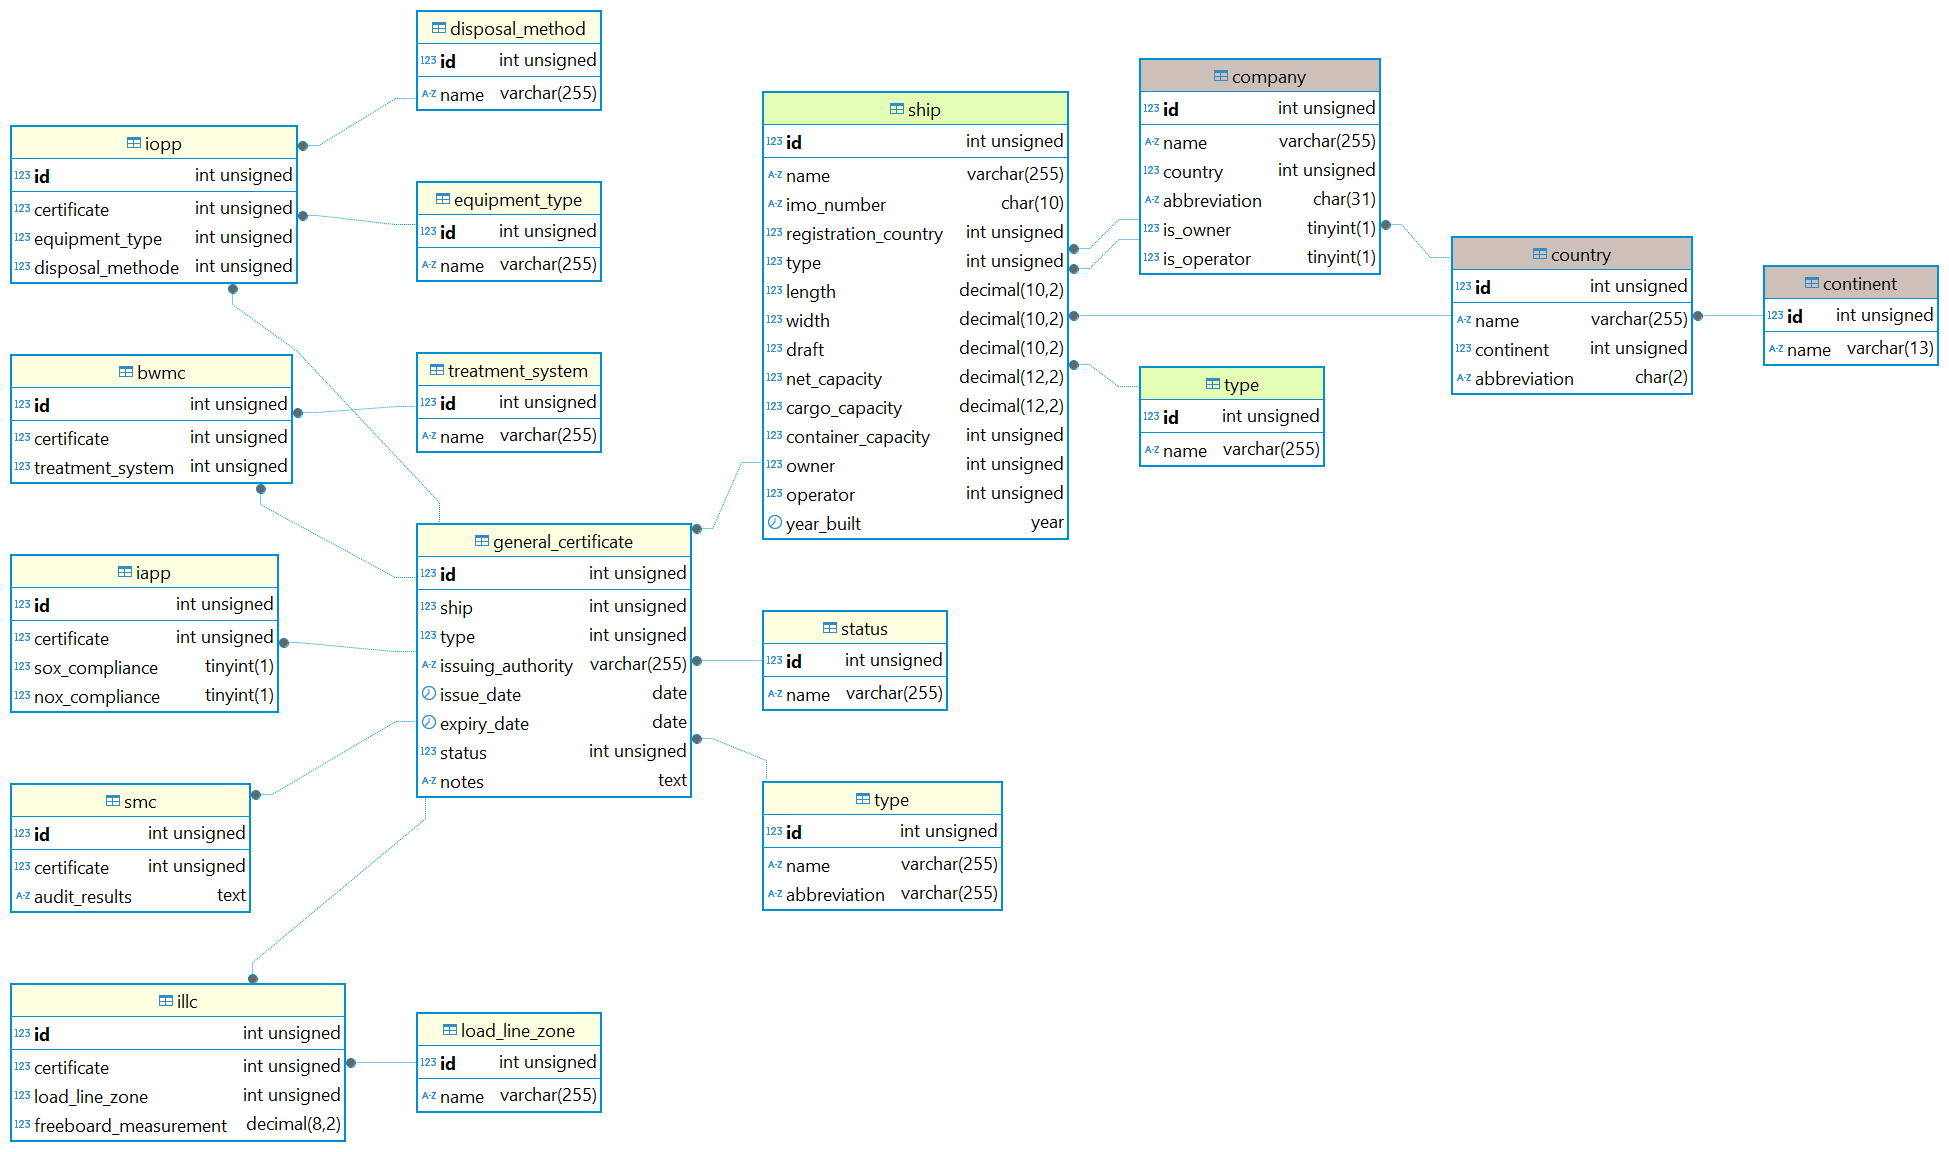
\includegraphics[width=1\textwidth,height=\textheight]{img/Schrempf/ship-erd.png}
\caption{ERD der Schiffdatenbank}
\end{figure}

Ein Schiff hat sehr viele Attribute wie seine Länge, Breite und Gewicht,
aber auch rechtlich verbindliche Angaben wie sein Typ oder verschiedene
Zertifikate die auf ihn zutreffen. In dieser Ausarbeitung ist die
Schiffsdatenbank nur ein unweigerliches Nebenprodukt der Gesamtarbeit.
Aufgrund dessen wurden nicht alle Zertifizierungen die ein Schiff haben
kann und manch andere Eigenschaften umgesetzt, sondern es wurde nur auf
das Nötigste begrenzt. Die hier implementierten Urkunden beschränken
sich auf:

\begin{itemize}
\tightlist
\item
  ILLC\footnote{International Load Line Certificate}
  {[}\protect\hyperlink{ref-imo}{53}{]}
\item
  IOPP\footnote{International Oil Pollution Prevention Certificate}
\item
  BWMC\footnote{Ballast Water Management Certificate}
\item
  IAPP\footnote{International Air Pollution Prevention Certificate}
  {[}\protect\hyperlink{ref-iapp}{54}{]}
\item
  SMC\footnote{Safety Management Certificate}
\end{itemize}

{[}\protect\hyperlink{ref-gpt-schiff-db}{55}{]}

\hypertarget{container}{%
\subparagraph{Container}\label{container}}

Jeder Container besitzt verschieden Parameter, welche ihn ausmachen.
Nicht nur seine Größe, sondern auch seine Materialbeschaffenheiten,
Tragfähigkeiten und Zulassungen sind ausschalggebend. In der hier
gestalteten Datenbank wurden Schema für allgemeine Containerdaten
(\passthrough{\lstinline!container!}), Größenklassifikationen des
Containers (\passthrough{\lstinline!dimension!}), Zertifikate die der
Container haben muss (\passthrough{\lstinline!certificate!}) und für die
Herkunft des Behälters (\passthrough{\lstinline!corporation!}),
angefertigt.

\begin{figure}
\centering
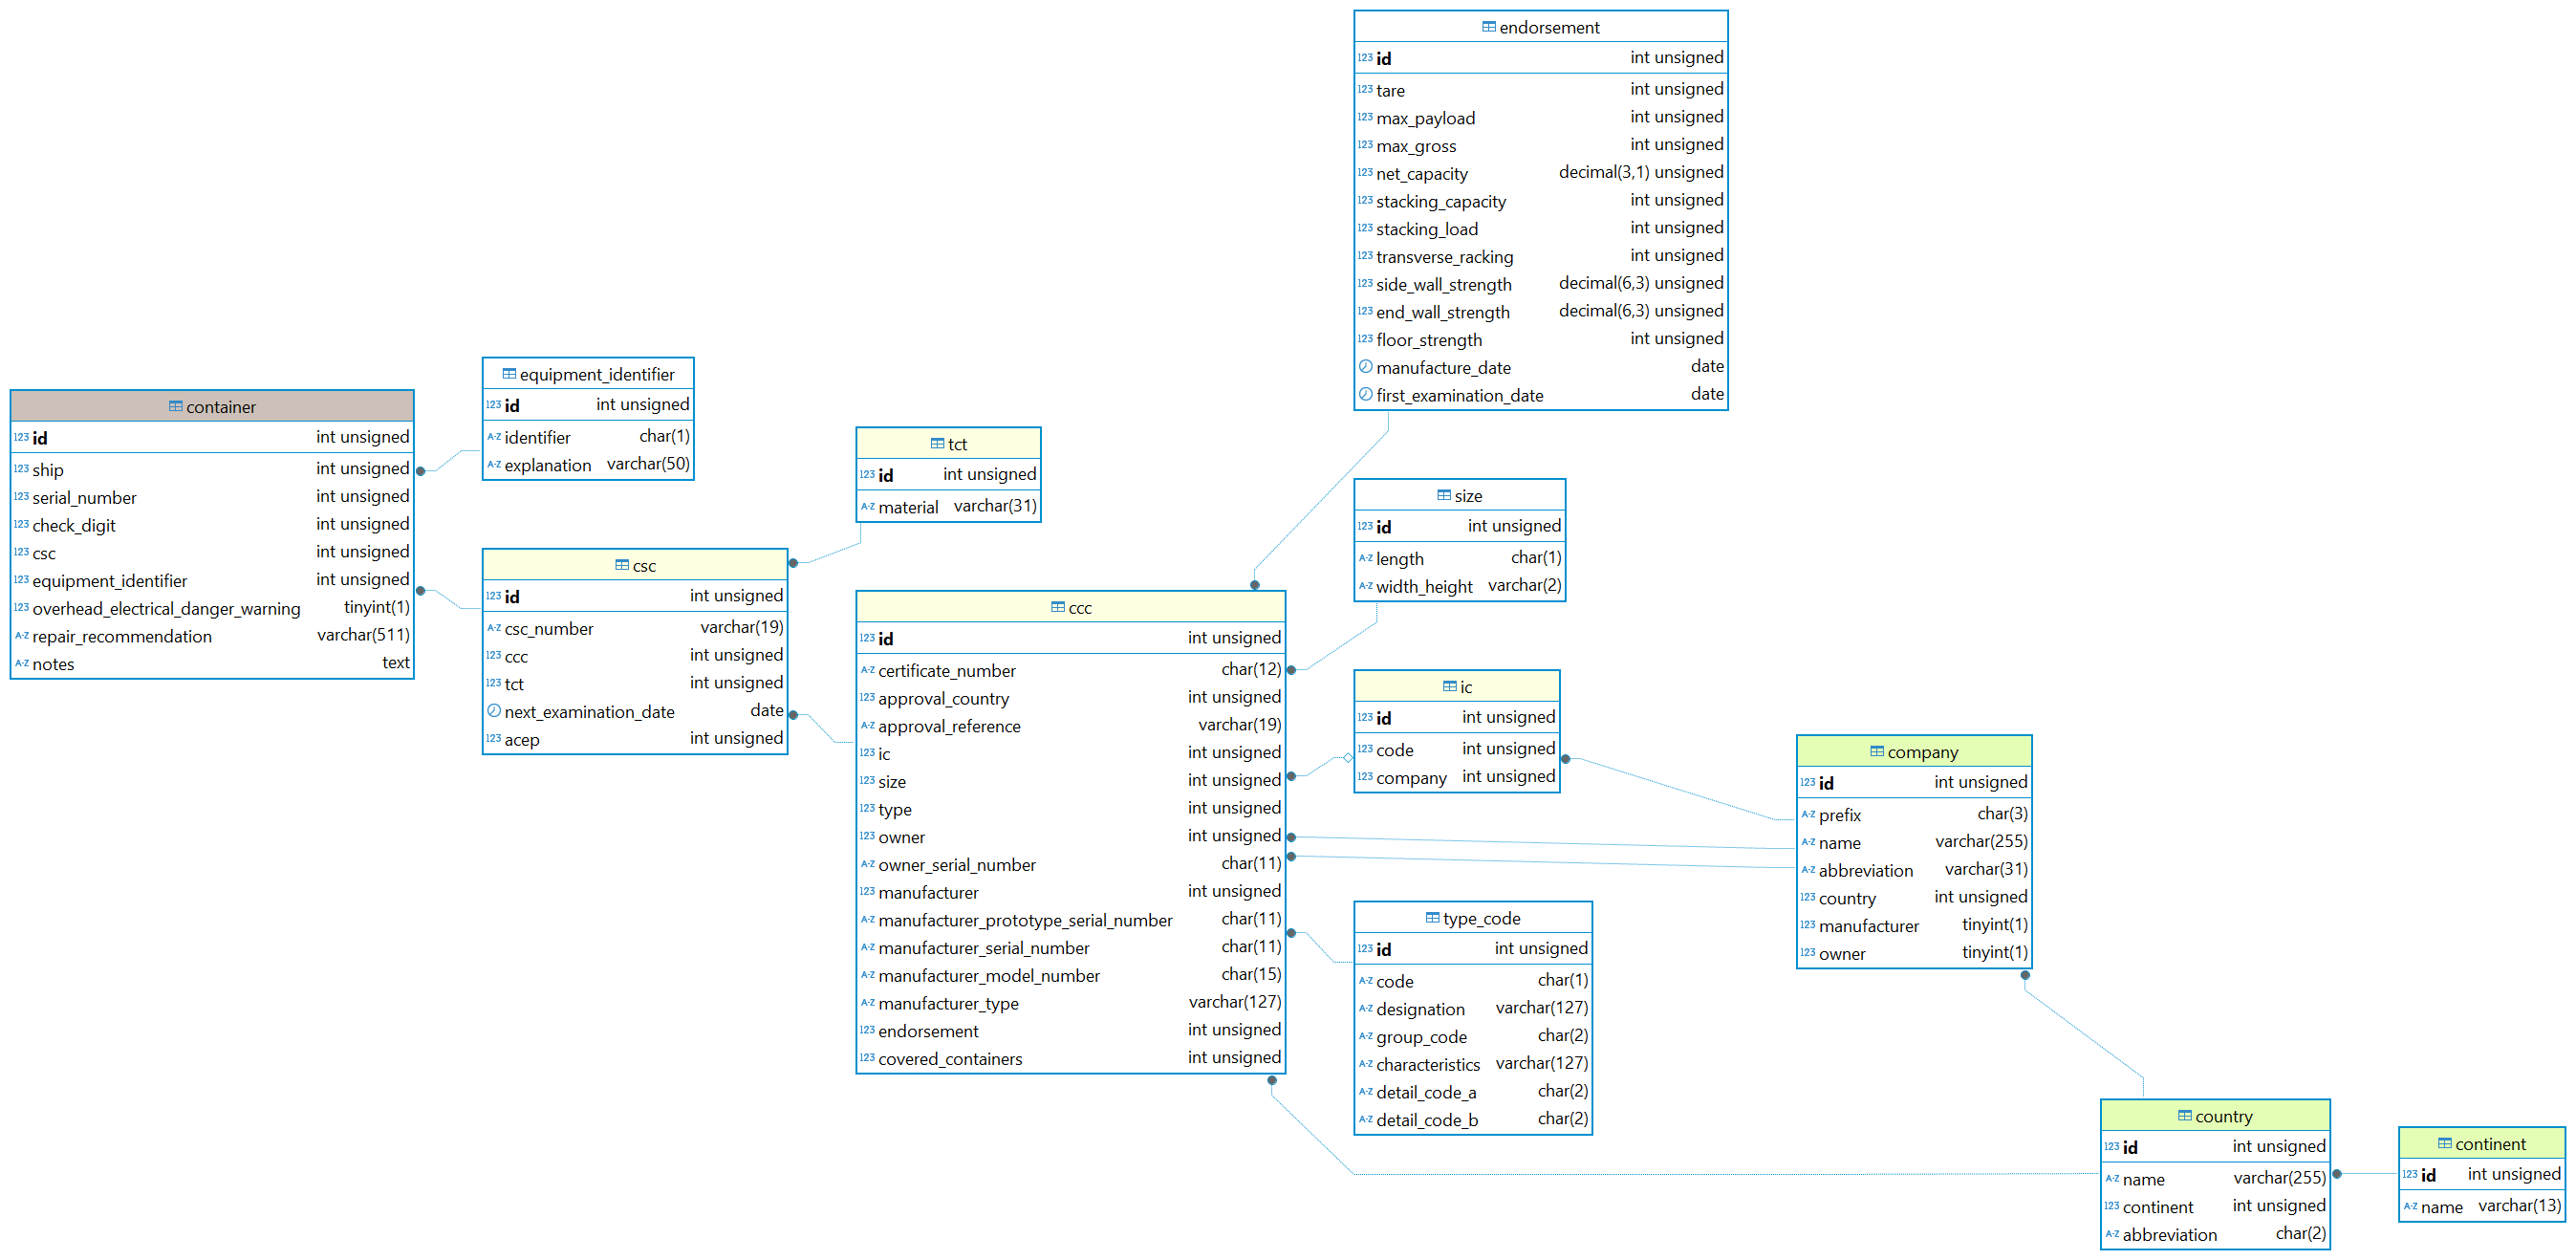
\includegraphics[width=1\textwidth,height=\textheight]{img/Schrempf/container-erd.png}
\caption{ERD der Containerdatenbank}
\end{figure}

Der Hauptfokus dieser Ausarbeitung liegt auf den Schiffcontainern. Diese
haben simple Attribute wie deren Abmessungen, Seriennummern und die
Firmen die sie hergestellt haben und besitzen.
{[}\protect\hyperlink{ref-bic-code}{56}{]}
{[}\protect\hyperlink{ref-icecargo}{57}{]} Doch wie bei den Schiffen
gibt es Zertifikate, die solch eine Transporteinheit standardisieren.
Dazu zählen:

\begin{itemize}
\tightlist
\item
  CSC\footnote{International Convention for Save Containers}

  \begin{itemize}
  \tightlist
  \item
    Vertrag der Vereinigten Nationen und der Internationalen
    Seefahrtsorganisation um standardisierte Regulationen bei Containern
    einzuführen. {[}\protect\hyperlink{ref-bic-code-csc}{58}{]}
  \end{itemize}
\item
  CCC\footnote{Container Construction Certificate}

  \begin{itemize}
  \tightlist
  \item
    Ist eine Zollplakette, in welcher die für diese Transporteinheit
    geltende Zollbestimmungen festgehalten sind.
    {[}\protect\hyperlink{ref-bic-code-csc}{58}{]}
  \end{itemize}
\item
  TCT\footnote{Timber Component Treatment}

  \begin{itemize}
  \tightlist
  \item
    Gemacht von der australischen Regierung um die konforme Beschichtung
    und Materialbeschaffenheit der Containerböden und Vermeidung eines
    möglichen Schädlingsbefalls durch in dem Holzboden übergebliebenen
    Parasiten sicherzustellen. {[}\protect\hyperlink{ref-tct}{59}{]}
  \end{itemize}
\item
  IC\footnote{InterContainer Codes}

  \begin{itemize}
  \tightlist
  \item
    Diese Zertifizierung bescheinigt einen Container zum Transport auf
    der Schiene. {[}\protect\hyperlink{ref-ic-codes}{60}{]}
  \end{itemize}
\end{itemize}

\hypertarget{grenzwerte}{%
\subparagraph{Grenzwerte}\label{grenzwerte}}

In dieser Ausarbeitung geht es um die Überwachung eines Containers.
Diese Datenbank dient dem Zweck, um nicht nur dessen Messwerte
auszulesen, sondern auch um zu definieren, wann ein kritischer Wert
erreicht worden ist. In der hier gestalteten DB wurde ein Schema für die
Grenzwerte (\passthrough{\lstinline!threshold!}) angefertigt. Ein
Grenzwert wird mit seinem Bereich in dem er gültig ist, seinem
Erwartungswert, in welchen Bereich um den Erwartungswert der gelieferte
Wert sein soll und die Priorität des angegebenen Limits definiert.

\begin{figure}
\centering
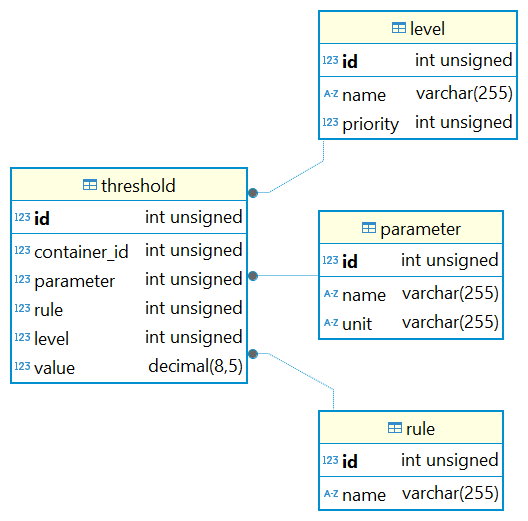
\includegraphics[width=0.5\textwidth,height=\textheight]{img/Schrempf/threshold-erd.png}
\caption{ERD der Grenzwertdatenbank}
\end{figure}

\hypertarget{user}{%
\subparagraph{User}\label{user}}

Um ein praktikable UI\footnote{user interface = Benutzeroberfläche}
bieten zu können, muss diese eine Login-Funktion beinhalten. Userdetails
müssen persistiert werden und die Datenbank dazu hat Schema für
allgemeine Userdaten und dessen Tokens (\passthrough{\lstinline!user!}),
Organisationsdaten des Benutzers (\passthrough{\lstinline!corporation!})
und die Rechte die der Anwender in der Applikation hat
(\passthrough{\lstinline!privilege!}). Wenn ein Benutzer sich
erfolgreich angemeldet hat, wernde zwei Tokens, Access und Refresh, vom
Server erstellt. Wie dies geschieht wird später weiter erläutert. Im
nachstehenden ERD\footnote{Entity-Relationship-Modell} ist zu bemerken,
dass die Tabelle der User-Tokens keine Verbindung zu anderen Tabellen
hat und somit auch mit keinen anderen Daten verknüpft ist, zumindest
scheint es so. Im Token selbst wird die Information, welchen Benutzer
dieser Token gehört, welche Rechte damit verbunden sind und wie lange er
gültig ist, eingebettet.

\begin{figure}
\centering
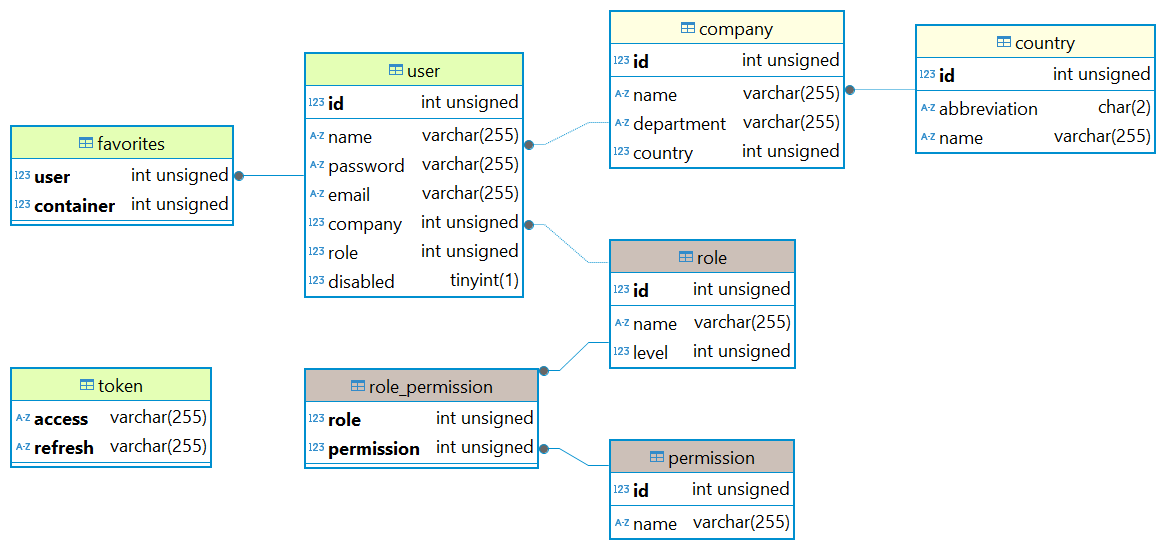
\includegraphics[width=1\textwidth,height=\textheight]{img/Schrempf/user-erd.png}
\caption{ERD der Benutzerdatenbank}
\end{figure}

\hypertarget{influxdb}{%
\paragraph{InfluxDB}\label{influxdb}}

Wir verwenden MQTT um Daten vom Prototyp zum Server zu bekommen. Das von
uns entworfene Gerät sendet seine Messwerte an einen MQTT Broker. In
unserem Fall ist der Publisher der Hardware-Prototyp und der Subsciber
ist Telegraf. Telegraf ist ein Client, in dieser speziellen Variante
auch Scraper genannt, welcher von InfluxDB entworfen wurde um aktiv
Datenquellen anzuzapfen und die mittels einer Konfigurationsdatei
definierten Filter auf die Ursprünge anzuwenden und die dadurch
extrahierten Werte an eine beliebige Applikation weiterzuleiten.
Telegraf ist in der Programmiersprache Go verfasst und bietet unzählige
Plugins zum empfangen, verarbeiten, aufbereiten und weitersenden der
Daten an. Die Konfigurationen werden im TOML\footnote{Tom's Obvious,
  Minimal Language}-Syntax geschrieben. Hier wurden die Erweiterung für
MQTT, RegEx\footnote{regular expression} zum Topic-Struktur-Filtern und
InfluxDBv2 verwendet. Das Filtern der Topics hat den Sinn, dass man nur
die nötigsten Daten bekommt, Overhead reduziert und auch die einzelnen
Werte exakt zuweisen kann. Als erstes wird nach einem groben Gesamttopic
gefiltert und temporäre Tags zum weiterverarbeiten erstellt.

\begin{lstlisting}[caption={Filtern der Topics in Telegraf mittels Regex}]
[[processors.regex]]
  [[processors.regex.tags]]
    key = "topic"
    pattern = "^contrude/(\\d+)/(\\d+)/([^/]+)$"
    replacement = "$1,$2,$3"
\end{lstlisting}

Nur wird jeder temporäre Tag mit einem real-funcktionalen Tag
ausgewechselt. Dieser Prozess passiert drei mal. Für Schiff, Container
und der Art des Sensors. Hier wird beispielhaftg nur der Schiffstag
angeheftet. {[}\protect\hyperlink{ref-gpt-telegraf-regex}{61}{]}

\begin{lstlisting}[caption={Ersetzen der temporären Topic-Tags durch funcktionale Tags}]
[[processors.regex]]
  [[processors.regex.tags]]
    key = "topic"
    pattern = "^([^,]+),([^,]+),([^,]+)$"
    replacement = "$1"
    result_key = "ship"
\end{lstlisting}

Zum Schluss wird der transformierte Datensatz in die Datenbank
eingespeist. Hierbei müssen sowohl die Verbindungsdetails und
Anmeldedaten als auch die Datenbank und die Zeitstempelpräzesion bekannt
gegeben werden. Zum Sicherstellen, dass nur ausgewählte Datensätze in
die DB kommen, wird mittels Tagpass definiert, welchen Tag das Topic
haben muss, um gespeichert zu werden. Im folgenden Beispiel muss das
Topic den in der Umgebungsvariable
\passthrough{\lstinline!TEMPERATURE\_TAGPASS!} definierten Tagwert
haben, um in den zugehörigen Temperaturbucket zu gelangen.

\begin{lstlisting}[caption={Persistieren der Messwerte in die Datenbank}]
[[outputs.influxdb_v2]]
  urls = ["${INFLUX_URL}:${INFLUX_PORT}"]
  token = "${INFLUX_TOKEN}"
  organization = "${INFLUX_ORG}"
  bucket = "${TEMPERATURE_BUCKET}"
  precision = "s"
  
  # Only pass data where the sensor tag is temperature
  [outputs.influxdb_v2.tagpass]
    sensor = ["${TEMPERATURE_TAGPASS}"]
\end{lstlisting}

InfluxDB ist ein zeitreihenbasierte Datenbankmanagementsystem, in
welchem eine Datenbank Bucket heißt. In diesem hier benötigten
Anwendungsfall gibt es für jeden einzelnen Messwert jeweils einen
Bucket. Diese wären:

\begin{itemize}
\tightlist
\item
  temperature = Temperatur
\item
  humidity = Luftfeuchtigkeit
\item
  air\_pressure = Luftdruck
\item
  vibration = Vibration
\item
  longitude = Längengrad
\item
  latitude = Breitengrad
\item
  altitude = Seehöhe
\end{itemize}

Außerdem gibt es InfluxDBv1 und InfluxDBv2. Bei V1 muss man für
API-Zugriffe Benutzername und Passwort angeben, was unter Umständen eine
Sicherheitslücke sein kann. Bei V2 wird der Gesamte API-Verkehr über
Tokens geregelt. Ein entscheidender Unterschied ist auch die
Abfragesprache. V1 verwendet normales SQL, V2 hingegen verwendet Flux.
Dies führte zu einer erheblichen Perfomancesteigerung.
{[}\protect\hyperlink{ref-influx-v1-vs-v2}{62}{]} Flux ist eine SQL
ähliche Query-Sprache, jedoch sehr stark auf das Abfragen von Zeitreihen
optimiert. {[}\protect\hyperlink{ref-flux}{63}{]}

\hypertarget{grafana}{%
\paragraph{Grafana}\label{grafana}}

Grafana ist ein Open-Source-Monitoring-Tool. Sprich, man kann es zur
Datenvisualisierung verschiedenster Quellen und Eingabearten verwenden
und sogar Alarme ausgeben lassen, wenn gewisse Events auftreten oder
Werte aus der Reihe tanzen. Somit bietet Grafana nicht nur
Visualisierungsmöglichkeiten der beliebtesten Datenquellen an, sondern
auch ein Benachrichtigungsystem, welche es in Summe auch zu einem
bekannten Industriestandard gemacht haben. In Grafana werden Dashboard
erstellt und darin Panels. Ein Panel ist eine Art der Visualisierung.
Zum Beispiel Histogramme, Heatmaps oder Balkendiagramme.
{[}\protect\hyperlink{ref-grafana-general}{64}{]} Außerdem bietet es den
großen Vorteil, dass Dashboards und Panels als JSON abrufbar sind und
somit sehr einfach importiert / exportiert werden können.

Um eine Visualisierung hinzuzufügen, muss man ein neues Dashboard und
darin eine neue Visualisierung erstellen. Nun wird man gefragt, die
Datenquelle zu konfigurieren. Hierfür wird das Plugin für InfluxDB
verwendet und eine neue Connection zu unserer Datenbank aufgebaut. Bei
den Dashboardeinstellungen kann man Variablen erstellen. Diese werden
hier in weiterer Folge als Platzhalter für die Schiff- und Container IDs
verwendet. Die Variablen bestehen jeweils aus einer Query, welche nur
die Werte mit den angegebenen Tags herausfiltern. Dies kann nur dann
geschehen, wenn die in InlfuxDB gespeicherten Werte überhaupt diese
Informationen als Tags bekommen haben.

\begin{figure}
\centering
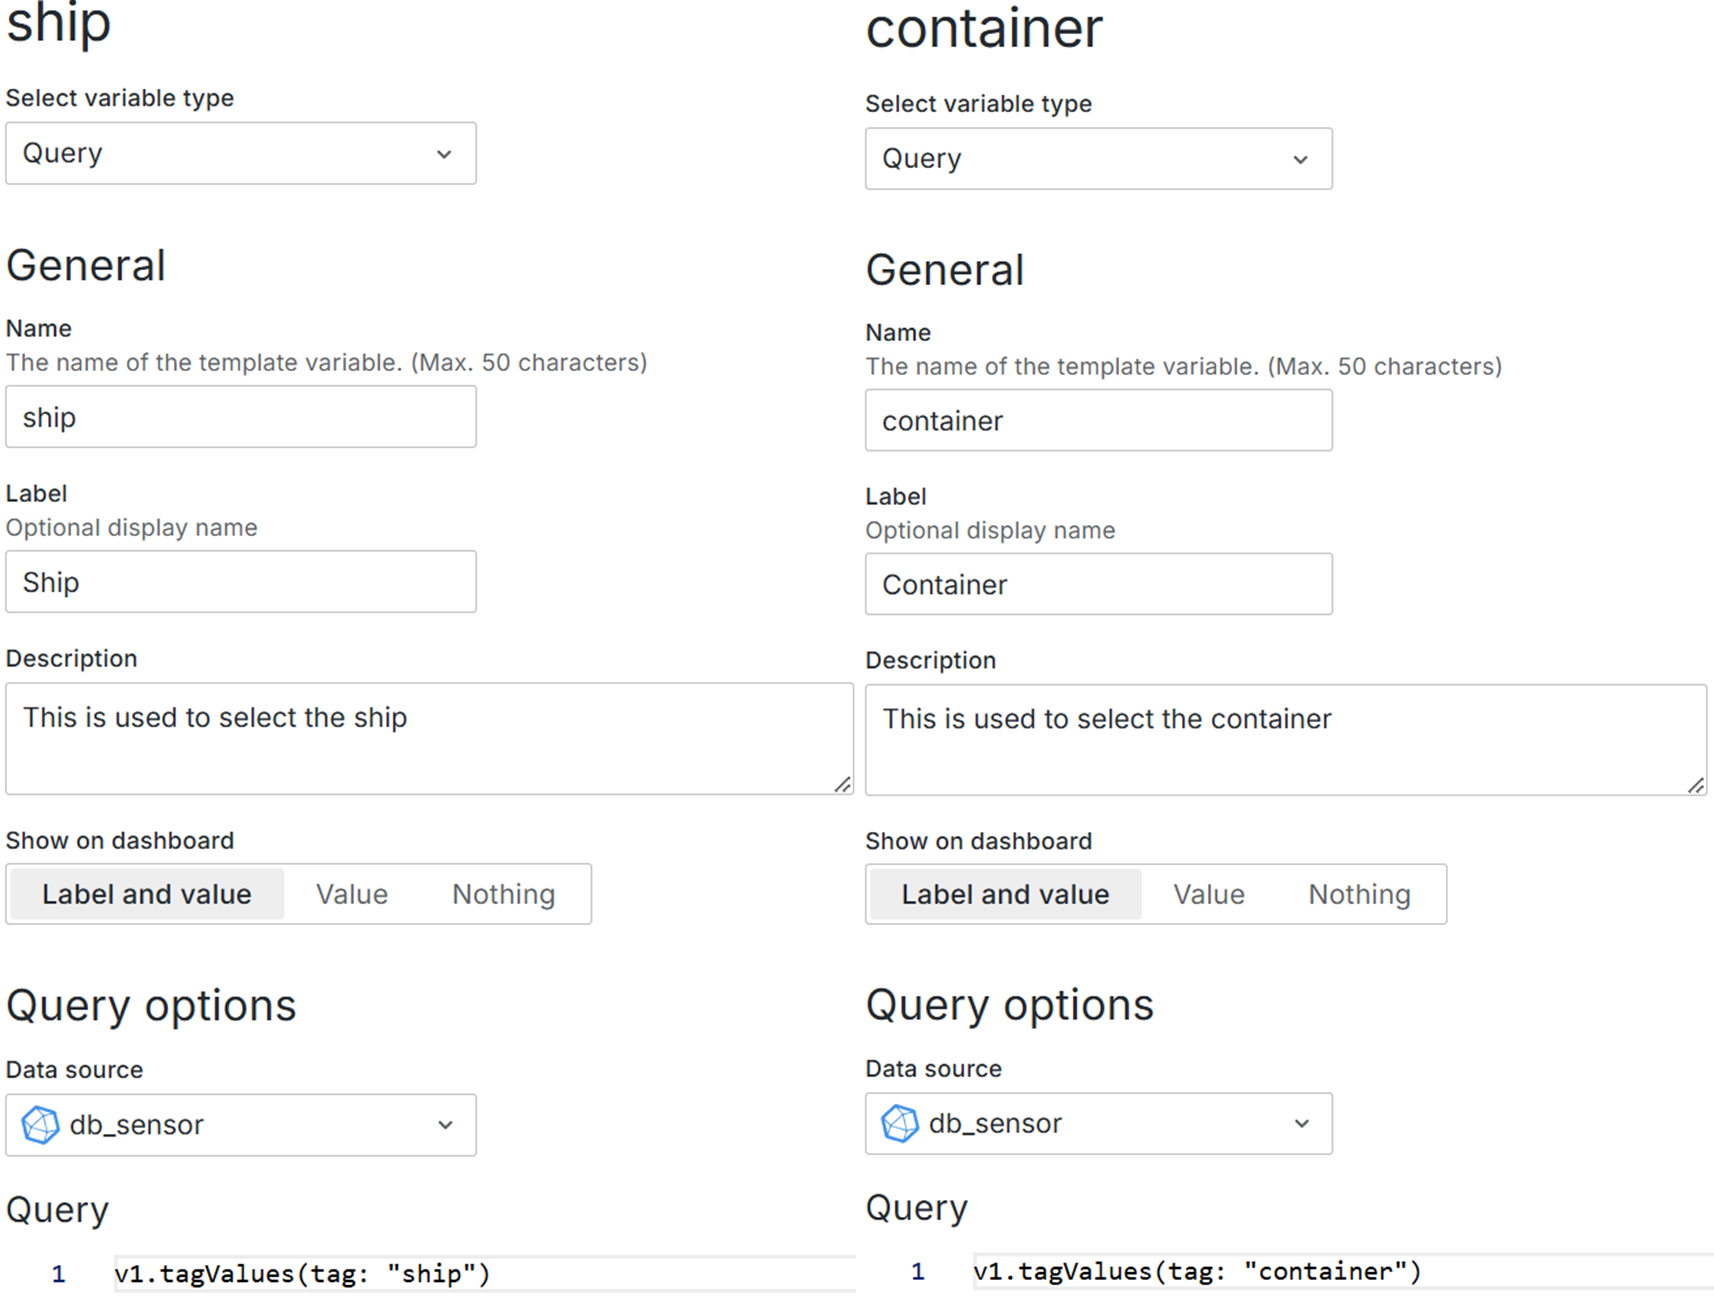
\includegraphics[width=1\textwidth,height=\textheight]{img/Schrempf/grafana-variables.png}
\caption{Grafana Variablen für Schiffe und Container
{[}\protect\hyperlink{ref-grafana-variables}{65}{]}}
\end{figure}

Nun sieht die leere Visualisierung (Panel) so aus:

\begin{figure}
\centering
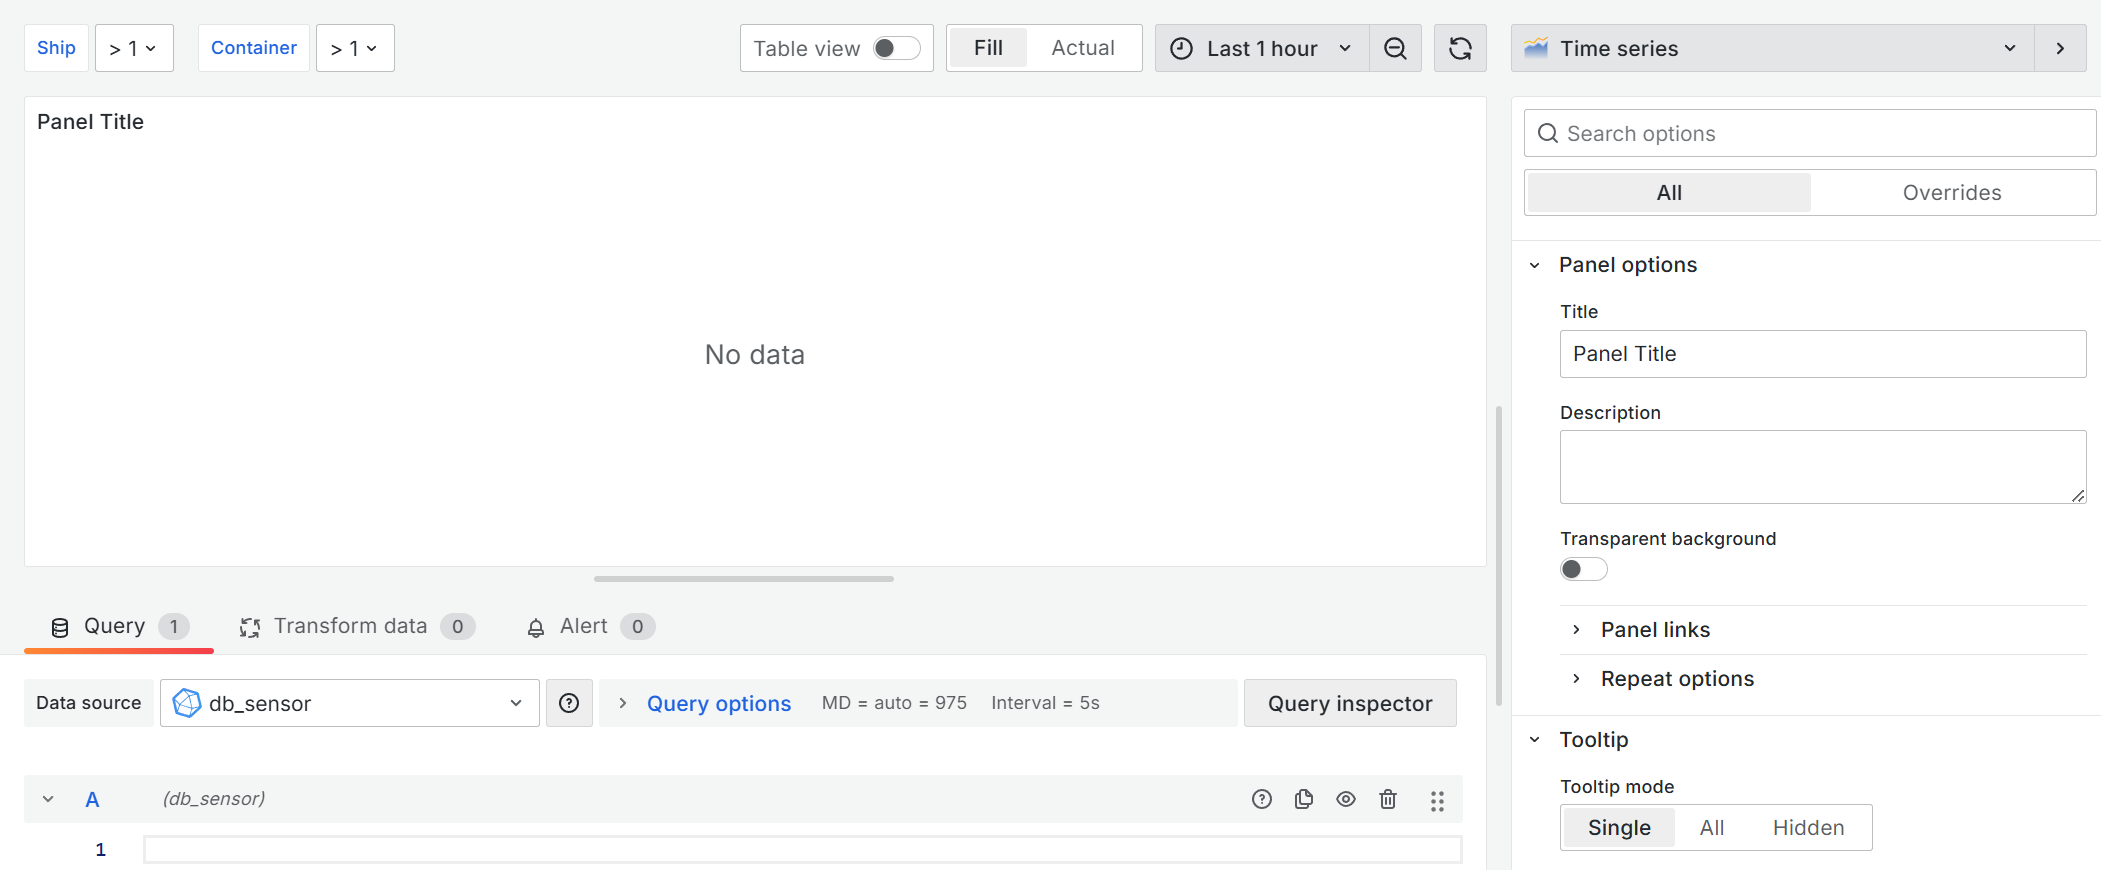
\includegraphics[width=1\textwidth,height=\textheight]{img/Schrempf/grafana-empty-panel.png}
\caption{Leeres Grafana Panel}
\end{figure}

Im unteren Teil kann man sehen, dass die zuvor ausgewählte Datensourse
da ist und das man diese mittels Flux-Queries abfragen kann. Um ein
Panel zur Temperaturvisualisierung zu gestalten, kann man die unten
angegebene Query verwenden. Der Zeitraum wird im Panel selbst definiert
und die Variablen können mittels einem Dropdownmenüs angepasst werden.

\begin{lstlisting}[caption={Flux-Query für Temperaturwerte in Grafana}]
from(bucket: "temperature")
  |> range(start: v.timeRangeStart, stop: v.timeRangeStop)
  |> filter(fn: (r) => r["ship"] == "${ship}")
  |> filter(fn: (r) => r["container"] == "${container}")
\end{lstlisting}

Nur noch auf Refresh drücken und es sieht schon so aus:

\begin{figure}
\centering
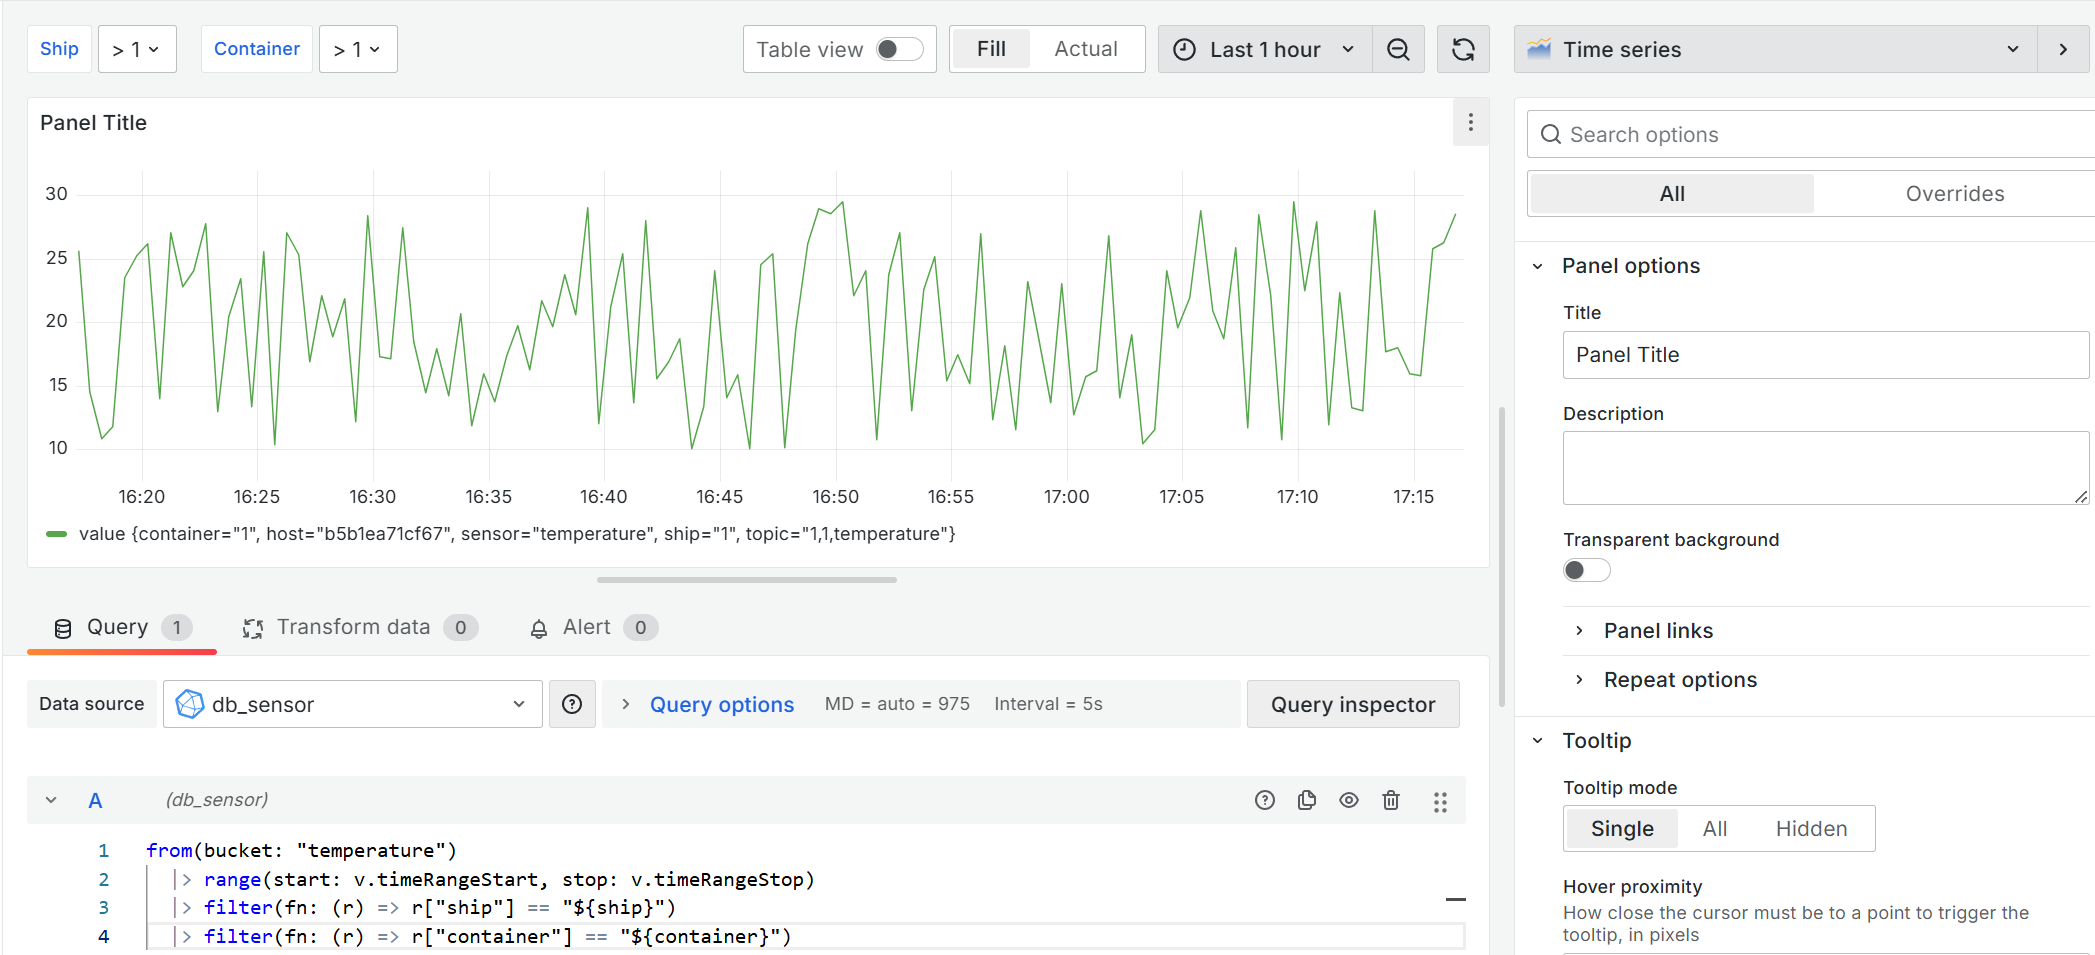
\includegraphics[width=1\textwidth,height=\textheight]{img/Schrempf/grafana-simple-panel.png}
\caption{Simples Grafana Panel}
\end{figure}

Nach weiteren Anpassungen wie Achsenbeschriftung, Diagrammtyp,
Diagrammtitel, Einheiten und Farben sieht das Diagramm in finaler
Version so aus:

\begin{figure}
\centering
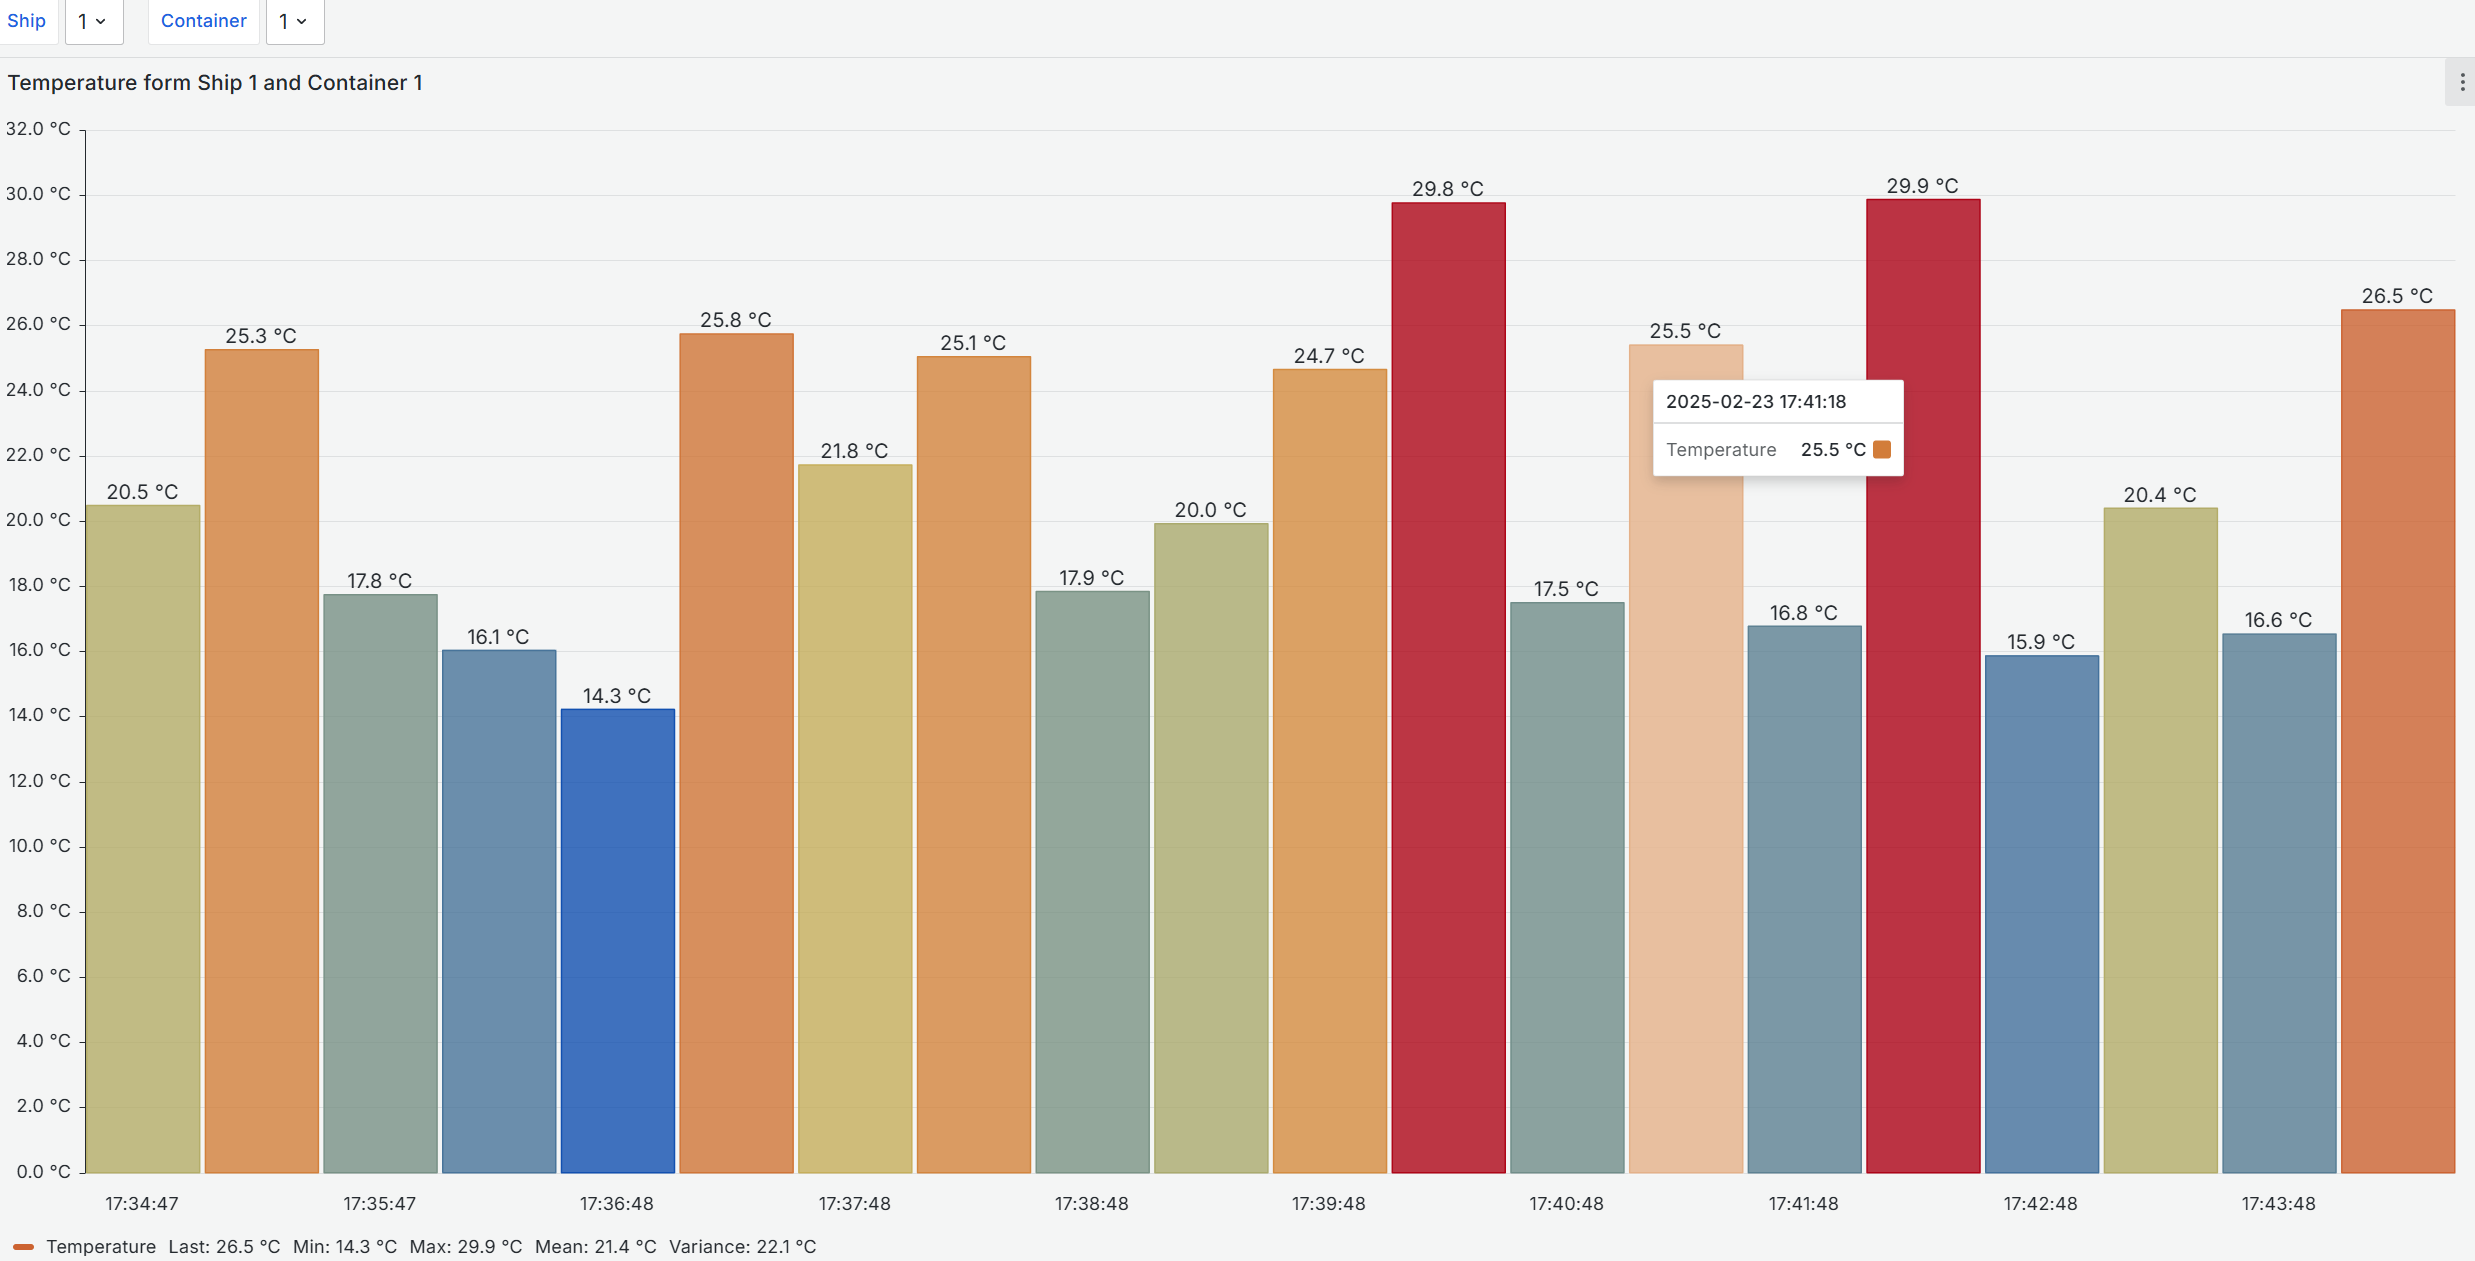
\includegraphics[width=1\textwidth,height=\textheight]{img/Schrempf/grafana-temperatur-panel.png}
\caption{Temperatur Grafana Panel}
\end{figure}

\hypertarget{continuous-integration-und-continuous-deployment-1}{%
\subsubsection{Continuous Integration und Continuous
Deployment}\label{continuous-integration-und-continuous-deployment-1}}

\hypertarget{docker-1}{%
\paragraph{Docker}\label{docker-1}}

In einer sich immer schneller ändernden Welt ist eine modulare Software
unausweichlich um Patches rasch einzuspielen, Sicherheitslücken zu fixen
und neue Features implementieren zu können. Da es leichter ist so ein
System einmal zu entwerfen und dann zu erweitern als ein bestehendes
Konstrukt umzugestalten, wurde hier vom Anfang an Docker verwendet um
genau so eine Architektur zu erzielen. Die gesamte Software ist in
Microservices unterteilt und kann theoretisch seperat betrieben werden.
Ausnahmen hinsichtlich der Abhängigkeit/Modularität bestehen nur bei
Anwendungen, die eine Andere voraussetzen z.B. ein Server eine
Datenbank. Anfangs wurde überlegt, für jeden einzelnen Service ein
Dockerfile zu schreiben. Ein Problem welches sich nicht lange darauf
einstellte war, wie man denn all die Anwendungen gleichzeitig hochfahren
könne. Eine Lösung bot hierbei Docker Compose. Nun kann man mehrere
Services in einer Datei definieren und mit einem Befehl hochfahren:
\passthrough{\lstinline!docker compose up!}. Da man in Docker Compose
zwar einen Service aus einem Image, welches in einem eigenen Dockerfile
beschrieben wurde, erstellen kann, dies jedoch bei uns keinen Sinn
hatte, wurde die Strategie dahin gehend verändert, dass nur noch das
Base-Image vom Docker-Hub verwendet und im gebotenen Rahmen abgewandelt
wurde. Wir haben uns für die zweite Version entschieden, da wird die
Base-Images nicht wirklich verändern, sondern eher Konfigurationen an
ihnen durchführen. Beispiele dafür sind Volume-Mounts, Entrypoints
anpassen oder Umgebungsvariablen setzen. Zusätzlich erspart das, das
schreiben unzähliger Dockerfiles und man kann alles übersichtlich in
einer Datei behalten.
{[}\protect\hyperlink{ref-gpt-server-structure}{66}{]} Ein guter
Vergleich für das gelingen unseres Ansetzes ist, dass zu Anfang nur drei
Services im Einsatz waren und nun sind wir bei zwölf, welche über den
Lauf der Zeit ihren Weg in unsere Anwendung gefunden haben und auch
leicht einzugliedern waren. Folgende Services sind final im Einsatz:

\begin{longtable}[]{@{}llll@{}}
\caption{Welche Images werden für welche Services
verwendet}\tabularnewline
\toprule
\begin{minipage}[b]{0.22\columnwidth}\raggedright
Image\strut
\end{minipage} & \begin{minipage}[b]{0.22\columnwidth}\raggedright
Usage\strut
\end{minipage} & \begin{minipage}[b]{0.22\columnwidth}\raggedright
Services\strut
\end{minipage} & \begin{minipage}[b]{0.22\columnwidth}\raggedright
Scope\strut
\end{minipage}\tabularnewline
\midrule
\endfirsthead
\toprule
\begin{minipage}[b]{0.22\columnwidth}\raggedright
Image\strut
\end{minipage} & \begin{minipage}[b]{0.22\columnwidth}\raggedright
Usage\strut
\end{minipage} & \begin{minipage}[b]{0.22\columnwidth}\raggedright
Services\strut
\end{minipage} & \begin{minipage}[b]{0.22\columnwidth}\raggedright
Scope\strut
\end{minipage}\tabularnewline
\midrule
\endhead
\begin{minipage}[t]{0.22\columnwidth}\raggedright
mysql:8.0.29\strut
\end{minipage} & \begin{minipage}[t]{0.22\columnwidth}\raggedright
MySQL Datenbanken\strut
\end{minipage} & \begin{minipage}[t]{0.22\columnwidth}\raggedright
Schiffe, Container, Grenzwerte, Benutzer\strut
\end{minipage} & \begin{minipage}[t]{0.22\columnwidth}\raggedright
Datenbanken\strut
\end{minipage}\tabularnewline
\begin{minipage}[t]{0.22\columnwidth}\raggedright
influxdb:2.7-alpine\strut
\end{minipage} & \begin{minipage}[t]{0.22\columnwidth}\raggedright
Zeitreihenbasierte Sensordatenbank\strut
\end{minipage} & \begin{minipage}[t]{0.22\columnwidth}\raggedright
InfluxDB\strut
\end{minipage} & \begin{minipage}[t]{0.22\columnwidth}\raggedright
Datenbanken\strut
\end{minipage}\tabularnewline
\begin{minipage}[t]{0.22\columnwidth}\raggedright
traefik:v3.1.5\strut
\end{minipage} & \begin{minipage}[t]{0.22\columnwidth}\raggedright
Reverse Proxy\strut
\end{minipage} & \begin{minipage}[t]{0.22\columnwidth}\raggedright
Traefik\strut
\end{minipage} & \begin{minipage}[t]{0.22\columnwidth}\raggedright
Backend\strut
\end{minipage}\tabularnewline
\begin{minipage}[t]{0.22\columnwidth}\raggedright
eclipse-mosquitto:openssl\strut
\end{minipage} & \begin{minipage}[t]{0.22\columnwidth}\raggedright
MQTT Broker\strut
\end{minipage} & \begin{minipage}[t]{0.22\columnwidth}\raggedright
MQTT\strut
\end{minipage} & \begin{minipage}[t]{0.22\columnwidth}\raggedright
Backend\strut
\end{minipage}\tabularnewline
\begin{minipage}[t]{0.22\columnwidth}\raggedright
telegraf:1.32-alpine\strut
\end{minipage} & \begin{minipage}[t]{0.22\columnwidth}\raggedright
Datenübermittelung von MQTT zu InfluxDB\strut
\end{minipage} & \begin{minipage}[t]{0.22\columnwidth}\raggedright
Telegraf\strut
\end{minipage} & \begin{minipage}[t]{0.22\columnwidth}\raggedright
Backend\strut
\end{minipage}\tabularnewline
\begin{minipage}[t]{0.22\columnwidth}\raggedright
node:22-alpine3.18\strut
\end{minipage} & \begin{minipage}[t]{0.22\columnwidth}\raggedright
JavaScript Applikationen\strut
\end{minipage} & \begin{minipage}[t]{0.22\columnwidth}\raggedright
Authentifizierung, REST-API, Webanwendung\strut
\end{minipage} & \begin{minipage}[t]{0.22\columnwidth}\raggedright
API, Frontend\strut
\end{minipage}\tabularnewline
\begin{minipage}[t]{0.22\columnwidth}\raggedright
grafana/grafana:main\strut
\end{minipage} & \begin{minipage}[t]{0.22\columnwidth}\raggedright
Datenvisualisierung\strut
\end{minipage} & \begin{minipage}[t]{0.22\columnwidth}\raggedright
Grafana\strut
\end{minipage} & \begin{minipage}[t]{0.22\columnwidth}\raggedright
Frontend\strut
\end{minipage}\tabularnewline
\bottomrule
\end{longtable}

Da gewisse Anwendungen vertrauliche Informationen benötigen wie
Passwörter, Tokens und Webaddressen wurden diese in
Envirnoment-Variable-Files gespeichert. Diese Datei wird in dem Docker
Compose Abschnitt \passthrough{\lstinline!env\_file!} angegeben. Zu
jedem Service der sensible Umgebungsvariablen benötigt, gibt es eine
\passthrough{\lstinline!.env.template!} Datei. Diese Datei spezifiziert
welche Environments gesetzt gehören und fungiert somit als Template.
Hier werden noch keine sensiblen Informationen angegeben und somit kann
sie in das VCS hochgeladen werden. Nicht nur sensibles kann hier
mitgegeben werden, sondern es wird auch eine Differenzierung zwischen
Produktiv- und Entwicklungsumgebungen ermöglicht.

\begin{lstlisting}[caption={Definition einer Entwicklungsumgebung mittels Umgebungsvariablen}]
TRAEFIK_DOMAIN=traefik.localhost
API_DOMAIN=api.localhost
WEB_DOMAIN=www.localhost
\end{lstlisting}

\begin{lstlisting}[caption={Definition einer Produktivumgebung mittels Umgebungsvariablen}]
TRAEFIK_DOMAIN=traefik.contrude.eu
API_DOMAIN=api.contrude.eu
WEB_DOMAIN=www.contrude.eu
\end{lstlisting}

Alle Services haben die gleiche Struktur und gewisse Ähnlichkeiten im
Aufbau. Bei jedem Service wird das Attribut
\passthrough{\lstinline!restart!} auf
\passthrough{\lstinline!unless-stopped!} gesetzt. Dies bewirkt, dass bei
einem schwerwiegenden Fehler, welcher den Container zum Absturz bringt,
sich ein neuer Container hochfährt und Anfragen weitherin
entgegengenommen werden können. Somit ist der Grundstein für eine
Self-Healing-Architecture gelegt. Wenn Volumes gemounted werden, wird
zur besseren Kontrolle auch spezifiziert, ob dieser Mount Read-Only oder
Read-Write Rechte im Container selbst haben soll. Die Sektion
\passthrough{\lstinline!deploy!} ist noch ein überbleibes aus der Phase
des Projekts, als wir Docker Swarm verwendet haben, wird aber auch unter
der alleinigen Nutzung von Docke Compose, zwar weniger effektiv aber
doch, verwendet.

\hypertarget{mysql-1}{%
\subparagraph{MySQL}\label{mysql-1}}

Die MySQL Datenbank Services sind so konfiguriert, dass sie alle das
selbe Admin (root) Passwort, welches nach der Erstanmeldung geändert
werden muss, haben. Dies dient zur leichteren Erstkonfiguration und
bringt aufgrund des Einmalpassworts einen gewissen Sicherheitsfaktor
mit. Es werden immer zwei Volumemounts vollzogen. Einmal die Datenbank
selbst, welche im Container unter dem Pfad
\passthrough{\lstinline!/var/lib/mysql!} erreichbar ist, und als zweites
die Datenbankscripts zum initialisieren der DB. Der Standardport einer
MySQL Instanz ist 3306, aber aufgrund dessen, dass bei uns davon vier
verschiedene Stück exesiteren, wurden die Ports inkremental geändert.
Hier ein Beispiel der Container DB:

\begin{lstlisting}[caption={Definition eines MySQL Services}]
db_container:
  image: mysql:8.0.29
  environment:
    MYSQL_ROOT_PASSWORD: 123
    MYSQL_ONETIME_PASSWORD: "yes"
  restart: unless-stopped
  volumes:
    - ./databases/container/mysql:/var/lib/mysql:rw
    - ./databases/container/scripts:/docker-entrypoint-initdb.d/:ro
  ports:
    - "3308:3306"
  deploy:
    mode: global
\end{lstlisting}

\hypertarget{node.js}{%
\subparagraph{Node.js}\label{node.js}}

In Docker Compose gibt es ein Attribut
\passthrough{\lstinline!command!}, in dem man Shell Commands angeben
kann, die beim Starten des Containers ausgeführt werden sollen. Node.js
benötigt viele Packages im Hintergrund, welche im Ordner
\passthrough{\lstinline!node\_modules!} geladen werden. Die Packages
können sich aber je nach Betriebsystem und / oder Kernel unterscheiden.
Somit ist es am sinnvollsten, wenn man sie jedes mal frisch installiert.
Dies kann mit dem Command
\passthrough{\lstinline!sh -c 'npm install \&\& npm run build \&\& npm run dev -- --host'!}
erzielt werden.

\hypertarget{traefik}{%
\subparagraph{Traefik}\label{traefik}}

Traefik ist ein Open-Source Reverse Proxy und Load Balancer. Ein großer
Vorteil von Traefik zu anderen Konkurenten ist, dass man nicht viel
konfigurieren muss, da es aufgrund eines eigenen Service Discorvery
Modus die zu routenden Anwendungen automatisch erkennt. Außerdem muss
man sich nicht mehr mühselig SSL-Zertifikate kaufen, sondern kann diese
sich generieren lassen. Ein kleines Kontra bringt dieses Feature aber
mit sich: Da die Zertifikate nicht von einer offiziellen Autorität
ausgestellt werden, werden diese in den Browsern und von manchen
Libraries als unsicher geflaggt.
{[}\protect\hyperlink{ref-traefik-overview}{67}{]}

\begin{figure}
\centering
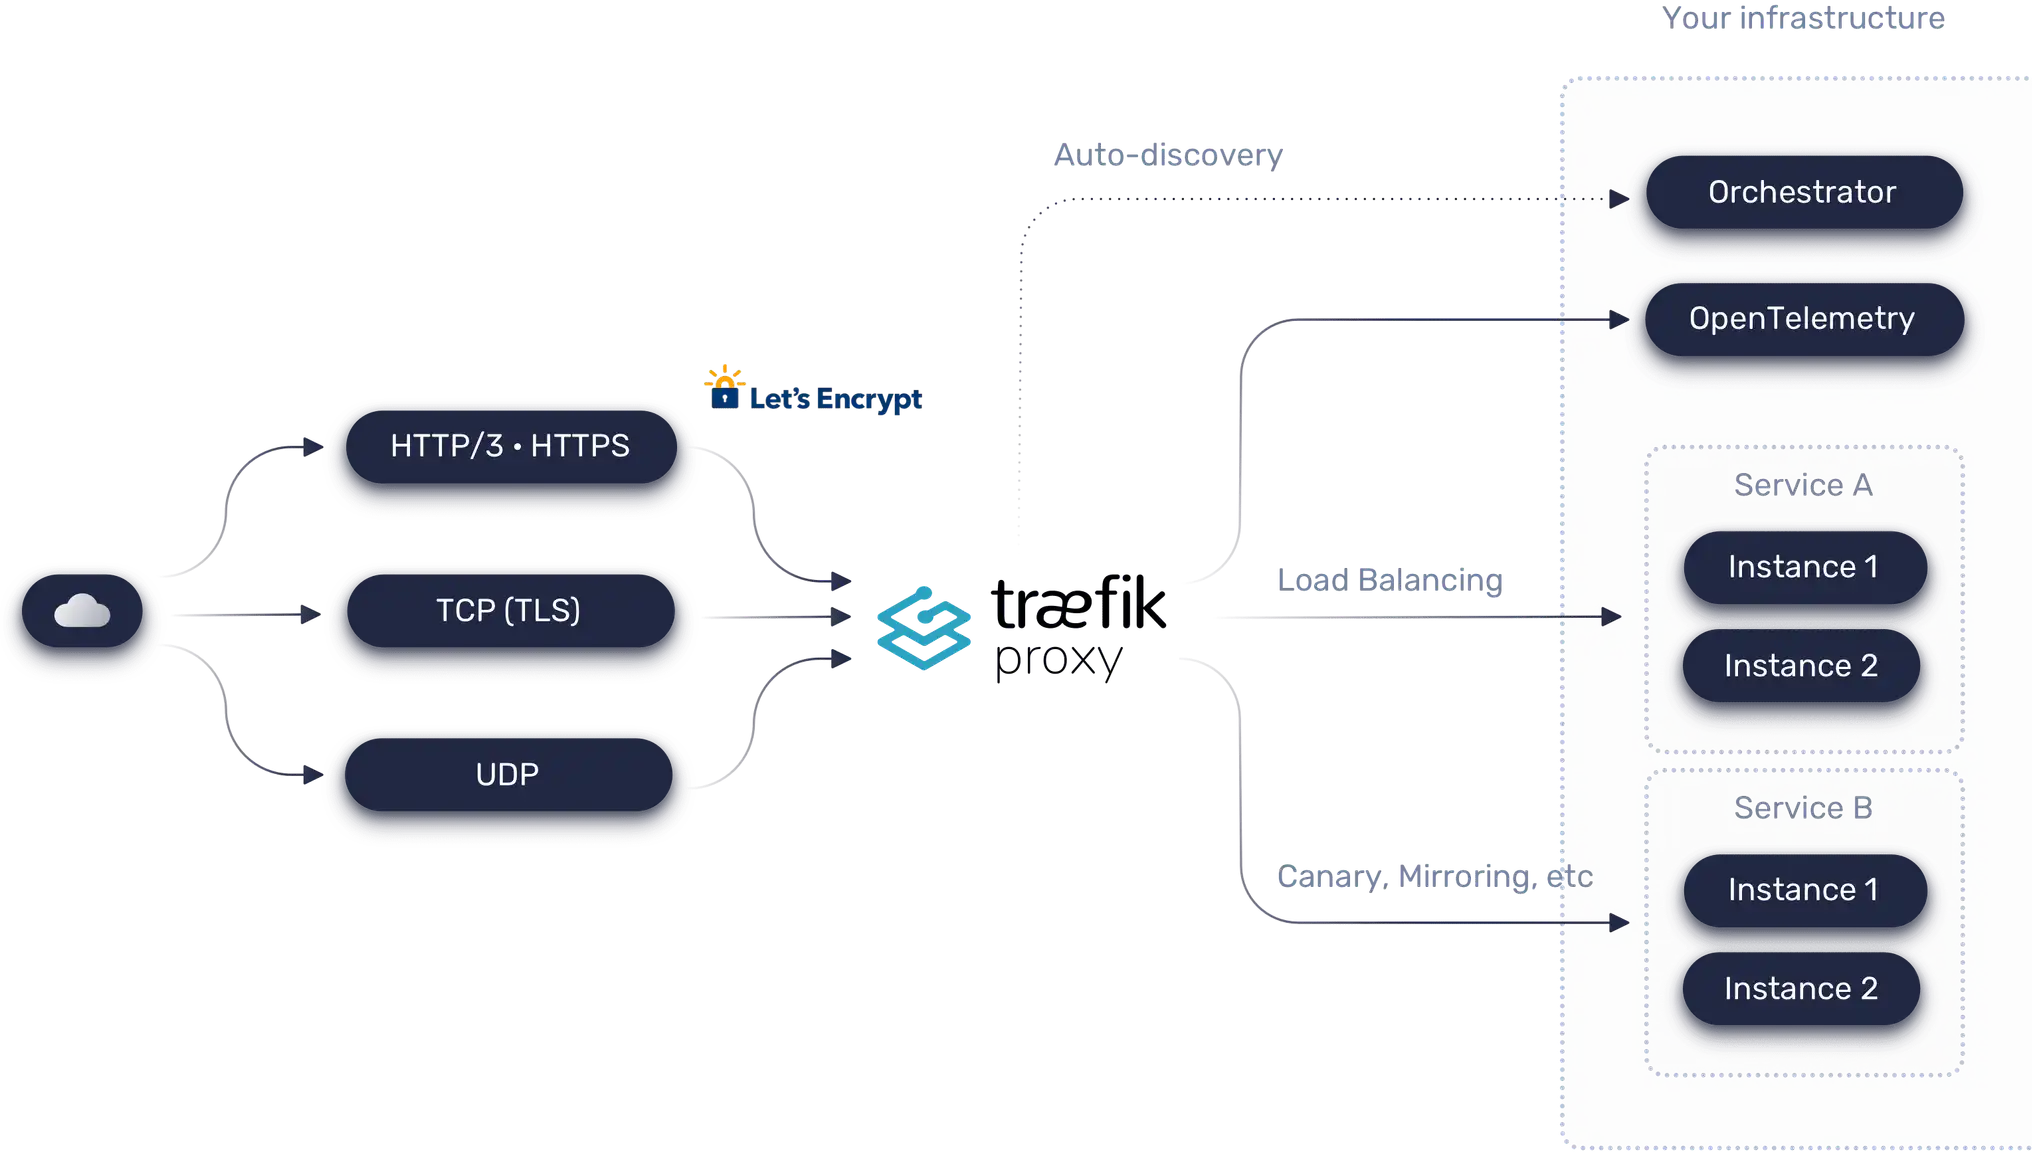
\includegraphics[width=1\textwidth,height=\textheight]{img/Schrempf/traefik-overview.png}
\caption{Traefik Übersicht
{[}\protect\hyperlink{ref-traefik-overview}{67}{]}}
\end{figure}

Um unsere Services sicher im Internet freizuschalten, verwenden wir die
automatisierte Generierung von TLS Zertifikaten von Traefik, welches mit
Let's Encrypt, einer Zertifizierungsauthorität, interagiert. Somit
upgraden wir von HTTP zu HTTPS auf.
{[}\protect\hyperlink{ref-traefik-lets-encrypt}{68}{]} Des Weiteren
haben wir Traefik so konfiguriert, dass jeglicher HTTP traffic auf HTTPS
umgeleitet wird. Dem Benutzer wird faktisch ein verschlüsselter
Datentransfer im Sinne des größeren Wohls aufgezwungen. Außerdem wird
zur Sicherheitssteigerung auch noch konfiguriert, dass nicht jeder
Service ins Web geschaltet werden soll, sondern nur jene, welche
expliziert erwähnt werden. Zusätzlich bietet Traefik ein Web-Dashboard
an, mit welchem man eine gute Übersicht über die verwalteten Services
erhält. Wir haben zwei API-Server. Einen zur Authentifizierung und einen
um die Daten der Schiffe, Container, Grenz- und Messwerte zu erhalten.
Um eine logische und (sicherheits-) technische Abgrenzung zu
ermöglichen, werden diese zwei seprat von einander betrieben. Um auch
einen Unterschied beim Aufrufen dieser im WWW\footnote{World Wide Web}
zu ermöglichen, gibt es eine Domain, aber verschiede Path-Prefixes unter
denen man die Services erreichen kann. Der Prefix für die
Authentifiziernungstelle lautet \passthrough{\lstinline!/auth!} und für
die restlichen Angelegenheiten \passthrough{\lstinline!/rest!}. Da es
mit der internen API Struktur der Server beim weiterrouten der Anfragen
Probleme gibt wenn davor etwas steht, was aber nicht im API-Server
selbst angegeben wurde, wird nach der Verarbeitung der Anfrage durch
Traefik der Path-Prefix wieder weggeschnitten.
{[}\protect\hyperlink{ref-gpt-traefik}{69}{]} Wichtig anzumerken ist
auch noch, dass wenn man Environment-Files für Traefik verwendet, diese
im exakt selben Ordner sein müssen wie die Docker Compose Datei in
welcher Traefik definiert ist, da ansonsten der Service die Datei nicht
lesen/interpretieren kann. Dies ist ein Sonderfall und trifft nur auf
den hier behandelten Dienst zu.

\begin{lstlisting}[caption={Definition eines Traefik Services}]
traefik:
  image: traefik:v3.1.5
  env_file: .env
  restart: unless-stopped
  command:
    - "--api.dashboard=true"
    - "--providers.docker=true"
    - "--providers.docker.exposedByDefault=false"
    - "--entrypoints.websecure.address=:443"
    - "--certificatesresolvers.myresolver.acme.httpchallenge.entrypoint=websecure"
    - "--certificatesresolvers.myresolver.acme.httpchallenge=true"
    - "--certificatesresolvers.myresolver.acme.email=${CERT_EMAIL}"
    - "--certificatesresolvers.myresolver.acme.storage=/letsencrypt/acme.json"
  ports:
    - "443:443" # only HTTPS traffic
  volumes:
    - "/var/run/docker.sock:/var/run/docker.sock:ro"
    - "./letsencrypt:/letsencrypt:rw" # storage for Let's Encrypt certificates
  labels:
    traefik.enable: true
    traefik.http.routers.api.rule: Host(`${TRAEFIK_DOMAIN}`) # hostname for dashboard
    traefik.http.routers.api.service: api@internal
    traefik.http.routers.api.entrypoints: websecure # reroute all traffic to https
    traefik.http.routers.api.tls.certresolver: myresolver
    traefik.http.routers.api.middlewares: traefik-auth
    traefik.http.middlewares.traefik-auth.digestauth.users: ${DASHBOARD_AUTH} # secure dashboard with login
    traefik.http.middlewares.traefik-auth.digestauth.removeheader: true
    traefik.http.middlewares.strip-prefixes.stripPrefix.prefixes: ${AUTH_PREFIX}, ${REST_PREFIX}
  deploy:
    mode: global
\end{lstlisting}

Den Diensten, welche freigeschaltet werden sollen, müssen nun Labels
hinzugefügt werden, welche dem Auto-Discovery von Traefik gewisse
Grundeinstellungen mitteilen.

\begin{lstlisting}[caption={Traefik Labels um einen Service zu konfigurieren}]
traefik.enable: true
traefik.http.routers.web.rule: Host(`${DOMAIN}`) # hostname
traefik.http.services.web.loadbalancer.server.port: ${PORT} # port
traefik.http.routers.web.entrypoints: websecure # reroute to https
traefik.http.routers.web.tls.certresolver: myresolver
\end{lstlisting}

\hypertarget{server}{%
\paragraph{Server}\label{server}}

Um unsere Services öffentlich zugänglich machen zu können, wurde ein
simpler headless Ubuntu Server mit der Version 24.04 auf einem Rasperry
Pi Model B mit 4GB RAM aufgesetzt. Dieses Gerät wurde dann mittels einer
öffentlichen IP\footnote{Internet Protocol} Addresse und einer damit
assoziierten Domain im Internet zugänglich gemacht. Ein verlässlicher
Remotezuugriff wird mithilfe der Installation von SSH\footnote{Secure
  Shell} ermöglicht. Da unsere gesamte Architektur auf Docker aufbaut,
wurde auch diese Software dort installiert.

\begin{figure}
\centering
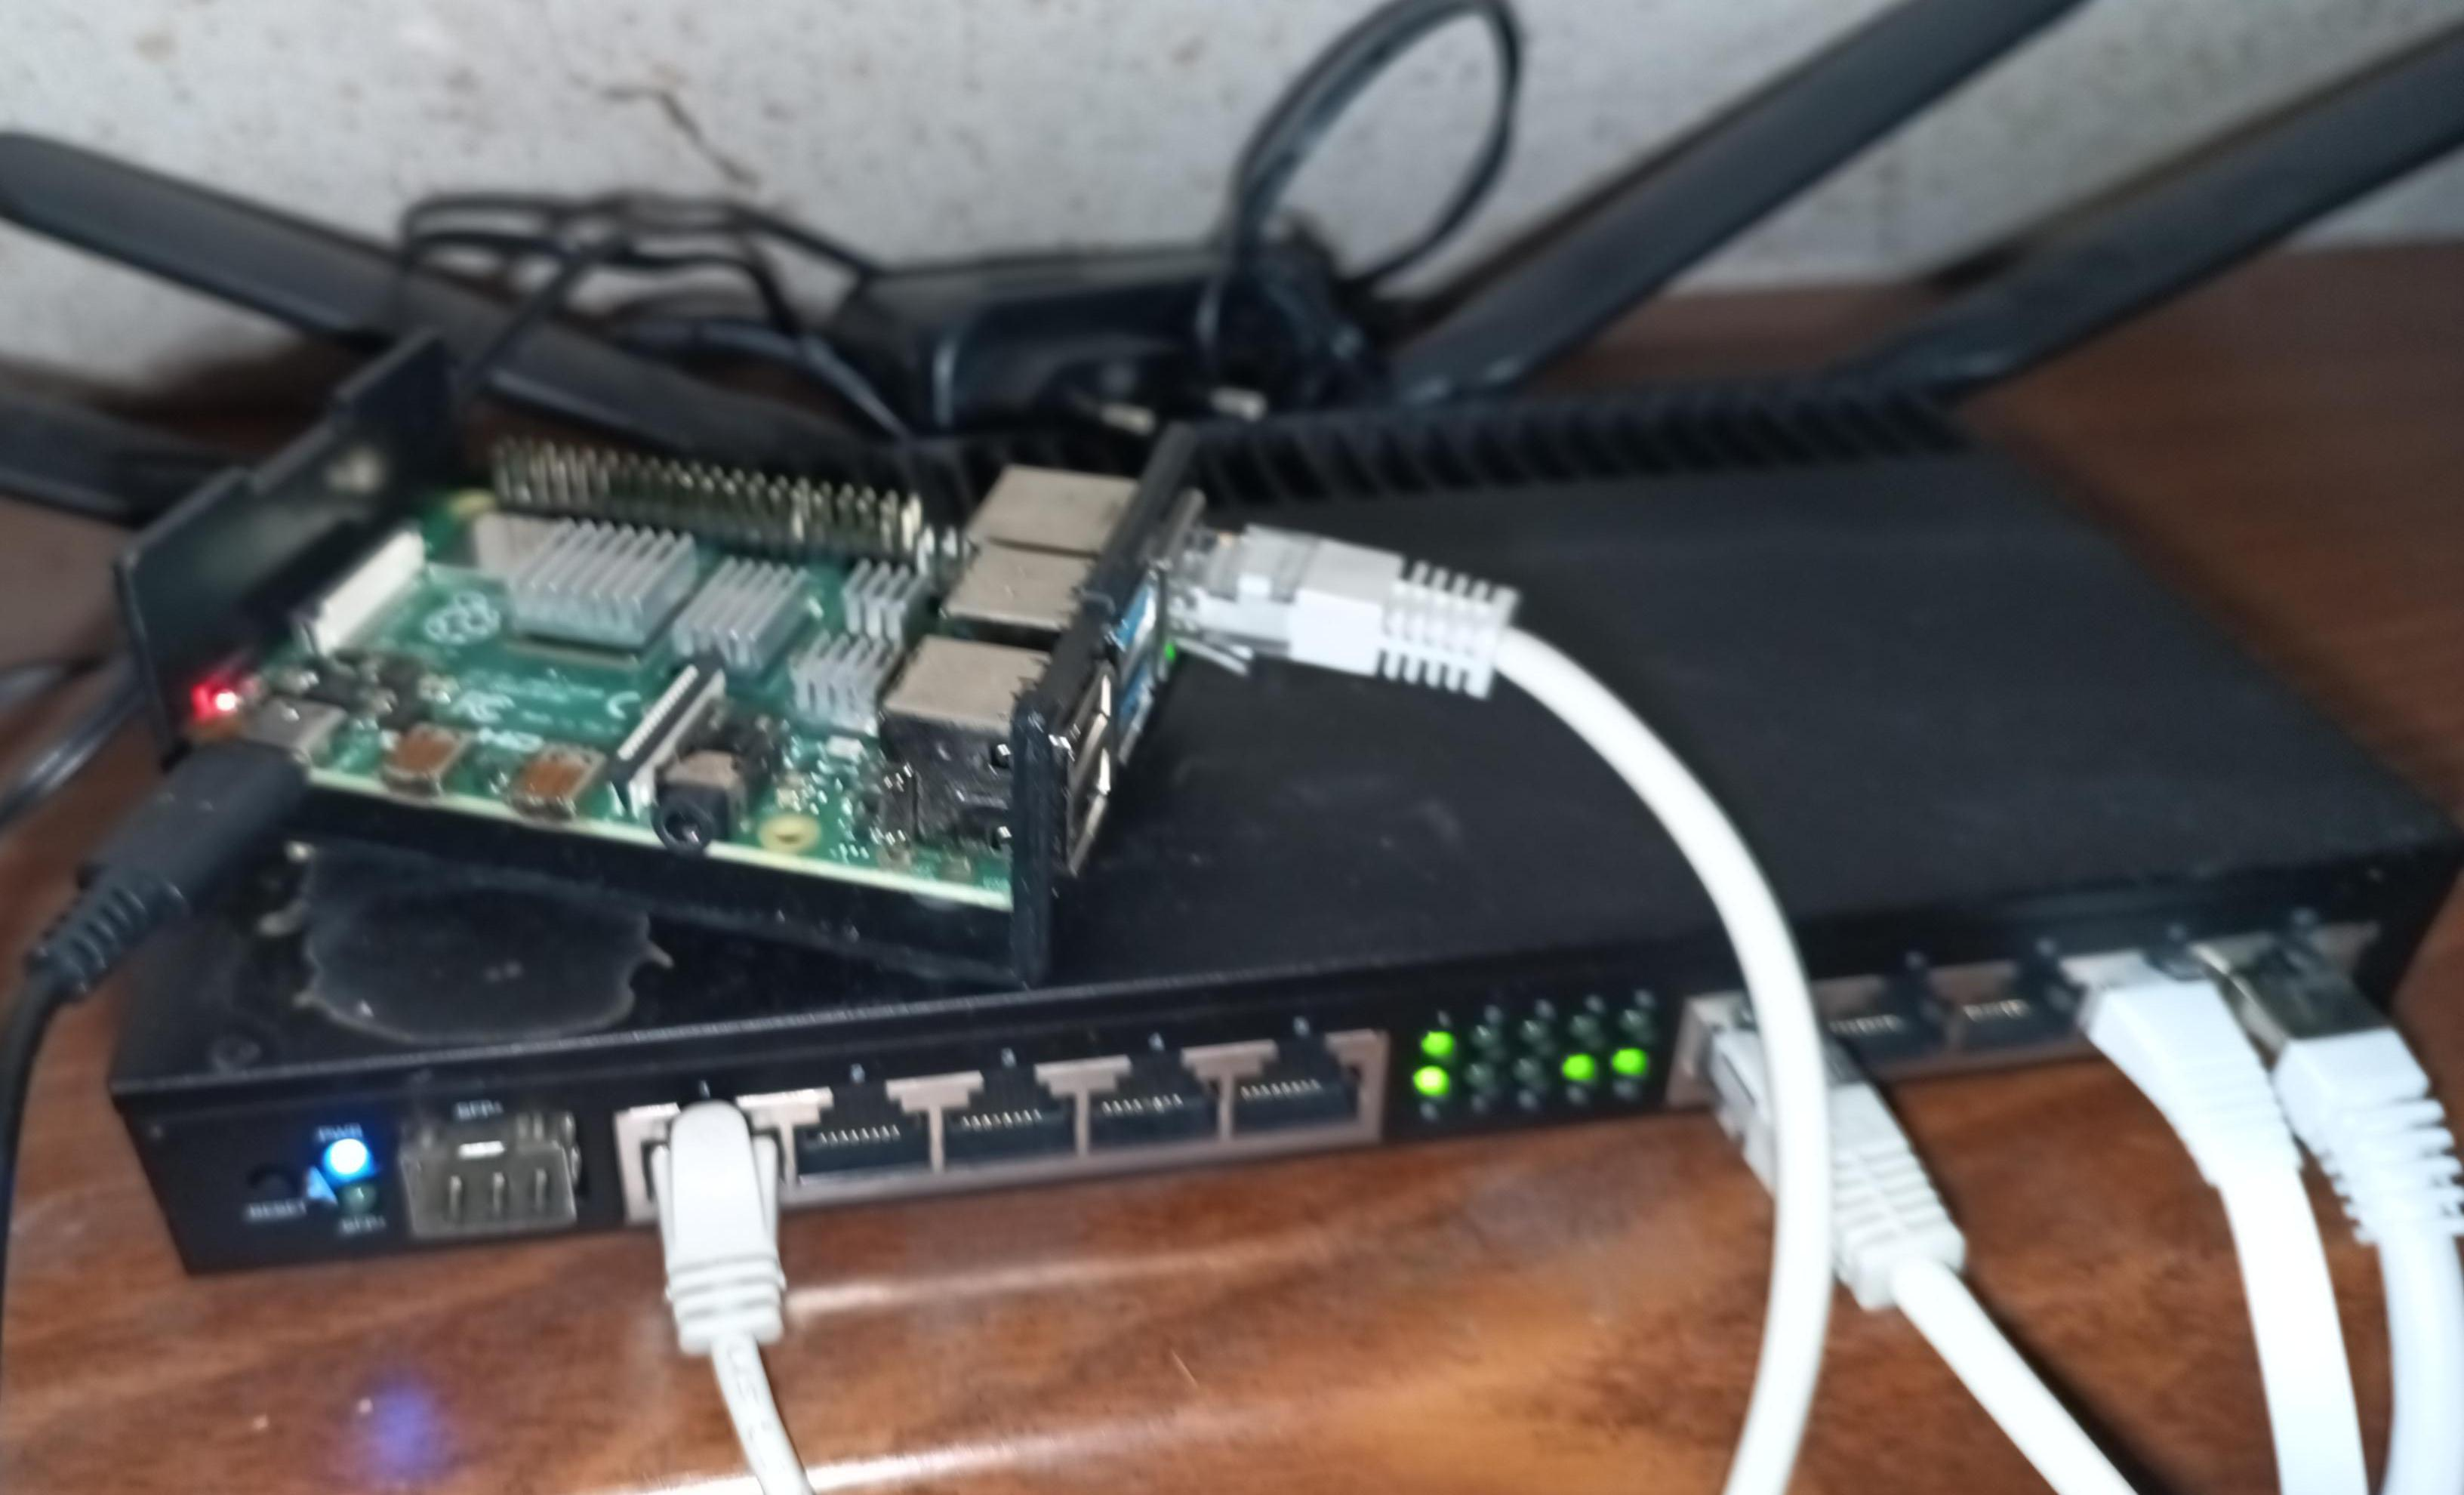
\includegraphics[width=1\textwidth,height=\textheight]{img/Schrempf/physical-server.png}
\caption{Server auf einem Raspberry Pi}
\end{figure}

\hypertarget{github-action}{%
\paragraph{GitHub Action}\label{github-action}}

Wir verwenden GitHub als VCS. Die durch diese Entscheidung möglich
gewordenen Automatisierungsmöglichkeiten haben wir sehr zu unserem
Vorteil genutzt. Es existieren zwei verschiedene Workflows um unser
Leben zu erleichtern.

\hypertarget{server-deploy}{%
\subparagraph{Server deploy}\label{server-deploy}}

Da sämtliche Anwendungen ihren eigenen Docker Container bzw. Eintrag im
Docker Compose haben, fällt es sehr leicht, unsere Arbeit zu deployen.
Es gibt verschiedene Ansätze solch eine Aufgabe zu realisieren, doch wir
haben uns dafür entschieden, eine SSH Verbindung zu unserem Server
aufzubauen, den geänderten Code von dort aus zu pullen und um
sicherzustellen das alle Dienste up to date sind die Docker Container
komplett herunter- und wieder hochzufahren. Dies bringt, eine für uns
vernachlässigbare, Downtime von 30s mit sich. Der angegebene Prozess
muss seitens Docker so ablaufen, da Codeänderungen sonst nicht direkt im
Container übernommen werden würden. Außerdem muss noch eine Änderung
beim Server vorgenommen werden, um diese Art des deployens zu
ermöglichen. Wenn man Docker Container auf Ubuntu starten bzw. stoppen
will, muss man dies mit erhöten Rechten, sprich
\passthrough{\lstinline!sudo!}, machen, was das eingeben eines Passworts
voraussetzt. Dieser Prozess beinhaltet eine Benutzerinteraktion und
lässt sich sehr schwer automatisieren. Das Benuzten einer GitHub Action
wird erschwert. Um das Problem zu umgehen, nutzen wir eine Datei des
Linuxsystems welche ermöglicht, gewisse Befehle ohne Sudo-Rechte
auszuführen. Sie befindet sich in \passthrough{\lstinline!/etc/sudoers!}
und man muss folgende Zeile anfügen, um ein Docker Compose Script ohne
Adminrechte ausführen zu können, wobei \passthrough{\lstinline!pi!} der
ausführende Benutzer ist:
\passthrough{\lstinline!pi ALL=(ALL) NOPASSWD: /usr/bin/docker compose up -d, /usr/bin/docker compose down!}.
{[}\protect\hyperlink{ref-sudo-no-pass}{70}{]} Der vollständige Workflow
besteht aus zwei Teilen, welche jeweils die korrespondierenden
Shellanweisungen ausführen.

\begin{enumerate}
\def\labelenumi{\arabic{enumi}.}
\tightlist
\item
  Das SSH Zertifikat des Servers zu den trusted Hosts in der GitHub
  Action VM hinzufügen.
\item
  Sich in den Server mittels SSH einloggen, den aktuellsten Stand pullen
  und die Docker Container herunter- und hochfahren.
\end{enumerate}

\begin{lstlisting}[caption={Updaten der Docker Container am Server}]
sshpass -p '${{ secrets.SSH_PWD }}' ssh -v -o StrictHostKeyChecking=no ${{ secrets.SSH_USER }}@${{ secrets.SSH_HOST }} <<'ENDSSH'
cd ${{ secrets.SSH_WORKDIR }}
git pull https://${{ secrets.SSH_GITHUB_PAT }}@github.com/BitSneak/Contrude.git
cd ./Server
sudo docker compose down
sudo docker compose up -d
ENDSSH
\end{lstlisting}

\hypertarget{super-linter}{%
\subparagraph{Super-Linter}\label{super-linter}}

Ein Linter ist eine Software, welche deinen Code analysiert und dich auf
Formatierungsfehler und Codekonsistenz hinweist. Seine Aufgabe ist es,
dich bei der Implementierung von Best-Practice Strategien zu
unterstützen und Programmfehler vorzubeugen. Für verschiedene
Programmiersprachen gibt es unterschiedliche Linter. Ein Super-Linter
ist nun eine Sammlung von Lintern und dient als Gesamtpacket. Somit muss
man nicht mehr für jede verwendete Programmiersprache einen
implementieren, sondern kann diese Collection verwenden um gleichzeitig
mehrere Sprachen abzudecken. Die zugehörige GitHub Action ist sehr
simpel und sieht folgendermaßen aus:
{[}\protect\hyperlink{ref-superlinter}{71}{]}

\begin{lstlisting}[caption={GitHub Superlinter}]
name: Super-Linter

on:
  push:

jobs:
  super-lint:
    name: Lint code base
    runs-on: ubuntu-latest
    steps:
      - name: Checkout Code
        uses: actions/checkout@v4

      - name: Lint Codebase
        uses: github/super-linter@v4
        env:
          DEFAULT_BRANCH: main
          GITHUB_TOKEN: $({ secrets.GITHUB_TOKEN })
\end{lstlisting}

\hypertarget{rest-api-1}{%
\subsubsection{REST API}\label{rest-api-1}}

Bei der Umsetzung der Backend Server haben wir uns für eine Trennung der
Authentifizierung und der Datenabfrage entschieden, da bei einer
Komprimierung einer dieser Komponenten die jeweils andere funktionsfähig
bleibt und sie auch getrennt von einander betrieben werden können, was
eine zusätzliche Sicherheitskomponente einführt. Außerdem wird
JavaScript als Programmiersprache und Node.js verwendet, da es
unzählige, für uns sehr nützliche, Libraries anbietet. Trotz der
logischen Trennung sind beide jedoch gleich aufgebaut:
{[}\protect\hyperlink{ref-medium-rest-api}{46}{]}

\dirtree{%
.1 src.
.2 db.
.3 connect.js.
.3 helper.js.
.2 errors.
.3 customErrors.js.
.2 middlewares.
.3 handleError.js.
.3 notFound.js.
.3 tryCatchWrapper.js.
.3 validateRouteParameter.js.
.2 resources.
.3 db.
.4 controller.js.
.4 helper.js.
.4 routes.js.
.1 ssl.
.1 .env.
.1 app.js.
.1 package.json.
}

In \passthrough{\lstinline!package.json!} werden die Grundzüge des
Projekts beschrieben. Welche Packages verwendet werden, welche Metadaten
vorhanden sind und der Einsprungspunkt. Da, aufgrund der besseren
Lesbarkeit, entschieden wurde, modular JavaScript (ES Module) zu
verwenden und dies auch spezifiziert werden muss, wurde
\passthrough{\lstinline!'type': 'module'!} in der oben angesprochenen
Datei eingegeben. Dies ermöglicht nun z.B.
\passthrough{\lstinline!import!} anstatt der CommonJS Variante
\passthrough{\lstinline!require()!} zu verwenden.

\passthrough{\lstinline!app.js!} ist der Einsprungspunkt der
Applikation. In ihr werden alle Routes importiert und Express
mitgeteilt, auch diese zu benutzten. Außerdem werden die
Standard-Error-Handler für die HTTP Codes 404 und 500 initialisiert und
der Server auf dem Port 80 gestartet.

\hypertarget{datenbanken}{%
\paragraph{Datenbanken}\label{datenbanken}}

Im Ordner \passthrough{\lstinline!db!} werden die Connection-Pools zu
den jeweiligen Datenbanken definiert. Ab der MySQL Version 8.0.16 sind
SSL-Zertifikate Pflicht zum Angeben beim Verbinden zur DB. Die
Zertifikate werden im gleichnamigen Ordner
\passthrough{\lstinline!ssl/db!} aufbewahrt. Dies im Hinterkopf
behaltend sieht ein Connection-Pool mit maximal 100 Connections
gelichzeitig folgendermaßen aus:
{[}\protect\hyperlink{ref-medium-rest-api}{46}{]}

\begin{lstlisting}[caption={MySQL Connection Pool für die Container DB}]
export const container = mysql
  .createPool({
    host: "db_container",
    port: 3306,
    database: "configuration",
    database: "certificate",
    database: "corporation",
    database: "dimension",
    user: "rest",
    password: process.env.DB_CONTAINER_PASSWORD,
    waitForConnections: true,
    connectionLimit: 100,
    ssl: {
      sslmode: "verify-full",
      ca: fs.readFileSync("./ssl/db/container/ca.pem"),
      cert: fs.readFileSync("./ssl/db/container/cert.pem"),
      key: fs.readFileSync("./ssl/db/container/key.pem"),
    }
  }).promise();
\end{lstlisting}

Hingegen solch eines Connection-Pools ist das Prozedere um einen für
eine InfluxDB herzustellen um einiges simpler, da man nur die Datenbank
URL und den passenden Token angeben muss:
{[}\protect\hyperlink{ref-influxdb-javascript}{72}{]}

\begin{lstlisting}[caption={InfluxDB Connection Pool für die Sensor DB}]
export const sensor = new InfluxDB({url: process.env.DB_SENSOR_URL, token: process.env.DB_SENSOR_TOKEN});
\end{lstlisting}

Alle Connection-Pools werden in der \passthrough{\lstinline!helper.js!}
genutzt werden. Dort sind Methoden definiert, welche einmal pro
Datenbankanfrage aufgerufen werden, sich für die Dauer der Anfrage eine
Connection aus dem Pool holen und nach Beendigung der Aufgabe diese
wieder freigeben. Folgendes Prinzip kann für alle SQL Datenbanken
verwendet und erweitert werden. Man erstellt eine Map aus den Namen,
Datentyp String, der Datenbanken in Kombination mit den Imports der
jeweiigen Datenbanken. In einer Funktion stellt man die Verbindung zur
DB her, formatiert mögliche Eingabeparameter des SQL Statements, führt
dieses in der Zugeteilten Datenbank aus und schließt die Connection.
Somit hat man einen Session Manager.

\begin{lstlisting}[caption={SQL Session Manager}]
import { container } from "./connect.js";

// Map from database name to database connection pool import
const dbMap = {
    "container": container,
};

// Generalized session function
const session = async function(sql, params, db) {    
    const con = await dbMap[db].getConnection();
    sql = params !== undefined ? dbMap[db].format(sql, params) : sql;
    
    const result = await con.query(sql);
    con.release();
    return result;
};

// Used general session to make a specific database session
export const container_session = async function(sql, params) {
    return session(sql, params, "container");
};
\end{lstlisting}

Eine No-SQL Datenbank kann weniger leicht generalisiert werden und muss
bis zu einem gewissen Grad spezifisch bleiben. Der Ansatz bleibt aber
wieder der Gleiche. Man übergiebt die auszuführende Query und bekommt
die Daten zurück. In InfluxDB gibt es pro Datensatz mehrere Spalten mit
verschiedensten Informationen. Jedoch werden nicht alle davon benötigt
und können der einfachheit halber nicht übernommen werden. Außerdem
können Daten in InfluxDB auch wieder über eine REST Schnitstelle
abgefragt werden, welche eine vorteilhafte Ebene an Abstraktion mti sich
bringt. In folgendem Beispiel wurde die Session auch gleich dazu
genutzt, Timestamps auf das richtige Format zu kriegen und gewisse
Datafields noch zu manipulieren / umzubenennen.

\begin{lstlisting}[caption={Flux Session Manager}]
export const sensor_session = async function(flux) {
    const api = sensor.getQueryApi(process.env.DB_SENSOR_ORG);

    return await new Promise((resolve, reject) => {
        const results = [];

        api.queryRows(flux, {
            next(row, tableMeta) {
                const result = tableMeta.toObject(row);

                // remove unnecessary fields
                delete result["result"];
                delete result["table"];
                delete result["_start"];
                delete result["_stop"];
                delete result["_field"];
                delete result["_measurement"];
                delete result["topic"];
                delete result["host"];

                // rename field _time to time
                result["time"] = result["_time"];
                delete result["_time"];
                // rename field _value to value
                result["value"] = result["_value"];
                delete result["_value"];

                // strip away unnecessary seconds
                result["time"] = result["time"].split('.')[0] + 'Z';
                // strip away unnecessary decimals
                result["value"] = parseFloat(result["value"]).toFixed(2);
                
                results.push(result); // add each row to the final results
            },
            error(error) {
                reject(error); // reject on error
            },
            complete() {
                resolve(results); // resolve with all collected results
            },
        });
    });
};
\end{lstlisting}

\hypertarget{middleware}{%
\paragraph{Middleware}\label{middleware}}

Eine Middleware ist prinzipiell dafür konzipiert, Daten zu
transformieren, überprüfen oder Fehler zu beheben oder zu werfen. Im
\passthrough{\lstinline!middlewares!} Ordner wird primär Error handling
und parameter checking betrieben. Mit
\passthrough{\lstinline!handleError.js!} wird eine Möglichkeit geboten,
indiviudelle Fehlermeldungen mit den korrespondierenden HTTP-Codes zu
werfen. Dies wird mit der Klasse \passthrough{\lstinline!CustomError!}
realisiert. Der \passthrough{\lstinline!tryCatchWrapper.js!} ist eine
Funktion, die einen try-catch Block beinhaltet und als Argument eine
auszuführende Funktion bietet. Wenn in der auszuführenden Funktion
Fehler geworfen werden, die dort nicht schon behandelt werden, schafft
diese Funktion sozusagen ein Schutzgitter, welches selbst bei critical
Errors die weitere Exekution des Programms ermöglicht. Es wird als
Wrapper angewandt. {[}\protect\hyperlink{ref-medium-rest-api}{46}{]}
URIs können Variablen in ihren Pathsegmenten beinhalten. Wenn solche vom
REST Endpoint benötigt werden, kann es zu schwerwiegenden Problemen
führen, wenn diese Variablen nicht gesetzt sind. Um dies vorzubeugen,
wurde \passthrough{\lstinline!validateRouteParameter.js!} geschrieben.
Es bietet eine Funktion, welche bei der Routendefinition als Middleware
eingespeist werden kann, um im Vorhinein zu überprüfen, ob die Variablen
gesetzt sind und wenn nicht, die Anfrage vorzeitig zu beenden.
Queryparameter und Routebodies muss man jedoch in der von der
Routedefinition aufgerufenen Funktion selbst nach Vorhandenheit prüfen.

\begin{lstlisting}[caption={Erstellen einer individuellen Error Klasse}]
export class CustomError extends Error {
    constructor(message, statusCode) {
      super(message);
      this.statusCode = statusCode;
    }
};
  
export const createCustomError = (message, statusCode) => {
  return new CustomError(message, statusCode);
};
\end{lstlisting}

\begin{lstlisting}[caption={Überprüfen der Vorhandenheit von Path Variablen bei REST Endpoints}]
const validateRouteParams = function(req, res, next) {
    // search for route parameters that are not set
    for (const [key, value] of Object.entries(req.params)) {
      // if a route parameter is not set, it starts with the place holder :
      if (value.startsWith(":")) {
        return next(createCustomError(`${key} parameter is required`, 400));
      }
    }
    next();
};
\end{lstlisting}

\hypertarget{routing}{%
\paragraph{Routing}\label{routing}}

Endpoints werden mittels Express in dem File
\passthrough{\lstinline!routes.js!} angefertigt. In dieser Dateie werden
alle von den Routen benötigten Funktionen von
\passthrough{\lstinline!controller.js!} importiert. In Letzterer wird
beschrieben, was welche Route machen soll bzw. die Funktion welche
hinter dieser Route steht. In der Ersten hingegen werden rein nur die
Routendefinitionen vorgenommen. Anzumerken ist hierbei, dass
Pathvariablen mit einem Dopppelpunkt und dem darauffolgenden
Variablennamen gekennzeichnet werden. Man kann auch direkt im Pathnamen
RegEx Ausdrücke anwenden.

\begin{lstlisting}[caption={Routing mittels Express}]
import express from "express";

import {
    getContainerById,
} from "./controller.js";
import validateToken from "../../middlewares/validateToken.js";
import validateRouteParams from "../../middlewares/validateRouteParameter.js";

const router = express.Router();

// execute the in the controller defined function when a request to this URI is sent
router.route("/container/:id").get(validateRouteParams, validateToken("select"), getContainerById);

export default router;
\end{lstlisting}

\hypertarget{authentifizierung}{%
\paragraph{Authentifizierung}\label{authentifizierung}}

Es gibt verschiedene Möglichkeiten eine API zugänglich zu machen. Sie
kann entweder für alle oder eingeschränkt verfügbar sein. Da in unserem
Anwendungsfall auch sensible Daten verarbeitet werden, haben wir uns für
eine beschränkte API entschieden. Wie schützt man sie nun? Mittels
Tokens. Was sind Tokens? Tokens sind zufällig generierte Schlüsselpaare,
welche Nutzerinformationen beinhalten. Diese darin gespeicherten
Informationen können nur dann ausgelesen werden, wenn man den Schlüssel
dekodieren kann. Deswegen ist es essenziell, um die Integrität des
Systems zu bewahren, dass man eine gute Verschlüsselung verwendet. In
diesem Fall hier werden die Libraries \passthrough{\lstinline!bcryptjs!}
zur Hash Erstellung und \passthrough{\lstinline!jsonwebtoken!} zur Token
Erstellung verwendet. Prinzipiell kann man auch nur einen JWT benutzen,
doch hier wird ein Access und Refresh Prinzip verfolgt. Es gibt nun zwei
Tokens. Einer, welcher jemanden Zugriff zu den Ressourcen ermöglicht und
einen welcher den Access Token nach Ablauf verlängern kann. Somit kann
ein Auto-Logout System implementiert werden. In dieser Ausarbeitung ist
der Access Token 15 min und der Refresh Token 20 min gültig. Solang eine
Aktivität des Benutzers verzeichnet wird, werden immer wieder neue
Tokenpaare generiert. Doch nach 20 min Inaktivität verliet der Benutzer
seinen Zugang und muss sich neu einloggen. Pro Tokenart gibt es
verschiedene Salts, welche mittels
\passthrough{\lstinline!require("crypto").randomBytes(64).toString("hex")!}
in Node.js generiert werden können. Die Passwörter der Benutzer werden
natürlich nicht im Reintext in den Datenbanken persitiert, sondern von
\passthrough{\lstinline!bcryptjs!} gehasht.
{[}\protect\hyperlink{ref-medium-auth-simple}{32}{]} Die Funktoin
\passthrough{\lstinline!bcryptjs.hash(input, n)!} nimmt zwei Parameter
an. Den zu hashenden Inputstring und die Anzahl der Hashdurchläufe n.~In
dieser Ausarbeitung wurden zehn Durchläufe festgelegt. Es gibt auch die
Möglichkeit, einen Input mittels der
\passthrough{\lstinline!bcryptjs.compare(input, hashedInput)!} Funktion
zu prüfen, ob er gleich dem zweiten schon gehashten Input ist. Die
wichtigsten Funktionen beim Authentifizierungssystem sind Login,
Validate Token, Refresh Token und Logout.

Die Login Funktion gibt einen Access- und Refresh Token als Response
zurück und nimmt im Routebody die ID des Benutzers und dessen Passwort
entgegen. Sie checkt in der Datenbank gegen, ob der Benutzer überhaupt
existiert, dann vergleicht sie das angegebene Passwort und das aus der
DB und speist schließendlich die Token mit den Benutzerdaten ein.
{[}\protect\hyperlink{ref-medium-auth-mysql}{73}{]}

\begin{lstlisting}[caption={Login Funktion}]
export const login = tryCatchWrapper(async function (req, res, next) {
  // extract data from request body
  const user = req.body.user;
  const pwd = req.body.password;

  // check if request body is present
  if (user === undefined) return next(createCustomError("user is required", 409));
  if (pwd === undefined) return next(createCustomError("password is required", 409));

  // sql statements
  const searchSql = "SELECT u.password, u.role, u.disabled FROM user.user u WHERE u.id = ? LIMIT 1";
  const insertSql = "INSERT INTO user.token VALUES (?, ?)";

  // check if user exists
  const [rows] = await session(searchSql, user);
  if (rows.length === 0) return next(createCustomError("User does not exist", 404));
  // check if user is disabled
  if (rows[0].disabled) return next(createCustomError("User is disabled", 401));

  const hashedPwd = rows[0].password;
  // check if the given password is correct
  if (await bcryptjs.compare(pwd, hashedPwd)) {
    // generate tokens
    const accessToken = generateAccessToken(user, rows[0].role);
    const refreshToken = generateRefreshToken(user, rows[0].role);

    // insert tokens into the database and send them back
    await session(insertSql, [accessToken, refreshToken]);
    return res.status(201).json({ accessToken: accessToken, refreshToken: refreshToken});
  } else {
    return next(createCustomError("Password incorrect", 401));
  }
});
\end{lstlisting}

\begin{lstlisting}[caption={Access Token Generierung}]
export const generateAccessToken = function(user, role) {
    return jwt.sign({user, role}, process.env.ACCESS_TOKEN_SECRET, {expiresIn: "15m"})
};
\end{lstlisting}

\begin{lstlisting}[caption={Refresh Token Generierung}]
export const generateRefreshToken = function(user, role) {
    return jwt.sign({user, role}, process.env.REFRESH_TOKEN_SECRET, {expiresIn: "20m"})
};
\end{lstlisting}

Die \passthrough{\lstinline!validateToken!} Funktion prüft, ob ein
Token, welcher im Authorization-Header mitgeführt wird, valide ist. Dies
beinhaltet, das nachschauen, ob der Token in der Datenbank vorhanden
ist, ob er noch eine zeitliche Gültigkeit aufweist und das Überprufen,
dass der Benutzer die für die Ressource benötigten Rechte aufweist und
auch nicht gesperrt ist. Ein zusätzlicher Parameter
\passthrough{\lstinline!isMiddleware!} wird aufgrund der Rückgabewerte
benötigt, um zu unterscheiden, ob die Funktion innerhalb des
Authentifizierungsservers oder von einer REST Abfrage aufgerufen wird.
Als Routeparameter nimmt sie die benötigte Rechtsstufe entgegen und gibt
entweder die HTTP-Codes 200 für valide (Zugriff gewährt) oder 403
(Zugriff verweigert) zurück.

\begin{lstlisting}[caption={Validate Token Funktion}]
export const validateToken = (requiredPermission, isMiddleware = true) => {
  return tryCatchWrapper(async (req, res, next) => {
    // retrieve token from authorization header
    const authHeader = req.headers["authorization"];

    if (authHeader == null) return next(createCustomError("Token not present", 400));
  
    const token = authHeader.split(" ")[1];
    if (token == null) return next(createCustomError("Token not present", 400));

    if (requiredPermission === null || requiredPermission === "") return next(createCustomError("Permission not present", 400));

    // sql statements
    const searchUserSql = "SELECT u.disabled FROM user.user u WHERE u.id = ? LIMIT 1";
    const searchTokenSql = "SELECT 1 FROM user.token t WHERE t.access = ? LIMIT 1";
    // query to check if the role has the required permission
    const searchRolePermissionSql = `
      SELECT 1
        FROM privilege.role_permission rp
        INNER JOIN privilege.role r
          ON rp.role = r.id
        INNER JOIN privilege.permission p
          ON rp.permission = p.id
        WHERE r.id = ? AND p.name = ? LIMIT 1`;

    // check if token is valid
    let [rows] = await session(searchTokenSql, token);
    if (rows.length === 0) return next(createCustomError("Token invalid", 401));

    // verify token
    const payload = jwt.verify(token, process.env.ACCESS_TOKEN_SECRET, (err, user) => {
      if (err) return next(createCustomError("Token expired", 403));
      req.user = user;
      return user;
    });

    // extract name and role from token
    const user = payload.user;
    const userRole = payload.role;

    // check if user is disabled
    [rows] = await session(searchUserSql, user);
    if (rows[0].disabled) return next(createCustomError("User is disabled", 401));

    [rows] = await session(searchRolePermissionSql, [userRole, requiredPermission]);

    // if there are any entries the user has the required permission
    if (rows.length > 0) {
      if (isMiddleware) return next();
      else return res.status(200).json({ message: "ok" });
    } else return next(createCustomError("Permission denied", 403)); 
  });
};
\end{lstlisting}

Die \passthrough{\lstinline!refreshToken!} Funktion ist dafür gedacht,
dass man ihr im Routebody den Refresht Token übergibt und wenn dieser
noch nicht abgelaufen ist, wird einem ein neues Paar an Access- und
Refresh Tokens übergeben und das alte Paar aus der Datenbank entfernt.

\begin{lstlisting}[caption={Refresh Token Funktion}]
export const refreshToken = tryCatchWrapper(async function (req, res, next) {
  // extract data from request body
  const refreshTokenOld = req.body.refreshToken;

  // check if request body is present
  if (refreshTokenOld === undefined) return next(createCustomError("refreshToken is required", 409));

  // sql statements
  const searchTokenSql = "SELECT 1 FROM user.token t WHERE t.refresh = ? LIMIT 1";
  const searchUserSql = "SELECT u.disabled FROM user.user u WHERE u.id = ? LIMIT 1";
  const updateSql = "UPDATE user.token t SET t.access = ?, t.refresh = ? WHERE t.refresh = ?";

  // check if token is valid
  let [rows] = await session(searchTokenSql, refreshTokenOld);
  if (rows.length === 0) return next(createCustomError("Refresh token invalid", 400));

  // check if refresh token is expired
  const payload = jwt.verify(refreshTokenOld, process.env.REFRESH_TOKEN_SECRET, (err, user) => {
    if (err) return next(createCustomError("Token expired", 403));
    else return user;
  });

  // retrieve user name from token
  const user = payload.user;
  const userRole = payload.role;

  // check if user is disabled
  [rows] = await session(searchUserSql, user);
  if (rows[0].disabled) return next(createCustomError("User is disabled", 401));

  // generate tokens
  const accessTokenNew = generateAccessToken(user, userRole);
  const refreshTokenNew = generateRefreshToken(user, userRole);

  await session(updateSql, [accessTokenNew, refreshTokenNew, refreshTokenOld]);
  return res.status(201).json({ accessToken: accessTokenNew, refreshToken: refreshTokenNew });
});
\end{lstlisting}

Um den Prozess der Benutzerabwicklung zu vervollständigen, gibt es noch
den Logout. Hier wird im Routebody wieder der Refresh Token übergeben
und die Tokenpaare des Nutzers aus der Datenbank entfernt.

\begin{lstlisting}[caption={Logout Funktion}]
export const logout = tryCatchWrapper(async function (req, res, next) {
  // extract data from request body
  const refreshToken = req.body.refreshToken;

  // check if request body is present
  if (refreshToken === undefined) return next(createCustomError("refreshToken is required", 409));

  // sql statements
  const searchSql = "SELECT 1 FROM user.token t WHERE t.refresh = ? LIMIT 1";
  const deleteSql = "DELETE FROM user.token t WHERE t.refresh = ?";

  // check if token is valid
  const [rows] = await session(searchSql, refreshToken);
  if (rows.length === 0) return next(createCustomError("Token invalid", 400));

  // check if refresh token is expired
  jwt.verify(refreshToken, process.env.REFRESH_TOKEN_SECRET, (err, user) => {
    if (err) return next(createCustomError("Token expired", 403));
  });

  // delete old token
  await session(deleteSql, refreshToken);
  return res.status(201).json({ message: "Logged out"});
});
\end{lstlisting}

Um diese Funktionen auch tatsächlich benutzen zu können, müssen sie
mittels Express in einer URI bereitgestellt werden können.

\begin{lstlisting}[caption=Authentifizierungsroutes]
router.route("/login").post(login);
router.route("/logout").delete(logout);
router.route("/token/:permission").get(validateRouteParams, (req, res, next) => validateToken(req.params.permission, false)(req, res, next));
router.route("/token/refresh").post(refreshToken);
\end{lstlisting}

\hypertarget{datenabfrage}{%
\paragraph{Datenabfrage}\label{datenabfrage}}

Im Vergleich zur allgemeinen Struktur gibt es beim Datenabfrageserver
noch eine weitere Datei namens
\passthrough{\lstinline!middlewares/validateToken.js!}. Diese bietet
eine Schnittstelle zum Authentifizierungsserver um die in den Header
mitgeführten Token zu prüfen. Sie leitet einfach die Anfrage weiter und
verarbeitet sie erst dann, wenn von
\passthrough{\lstinline!auth/token/:permission!} ein Statuscode 200
zurückgegeben wird. Die Struktur bleibt aber ansonten aufrecht. Damit
ist gemeint, dass in \passthrough{\lstinline!ressources!} nun weitere
Ordner für die jeweiligen Datenbanken gemacht wurden.

\dirtree{%
.1 resources.
.2 container.
.2 sensor.
.2 ship.
.2 threshold.
}

Vom Aufbau und der Funktionsweise gibt es kaum Unterschiede. Das einzige
was hier verschieden ist, ist die Sensordatenbank, welche mit InfluxDB
funktioniert. In \passthrough{\lstinline!helper.js!} wurden die Methoden
\passthrough{\lstinline!fluxQueryTimeRange!} für Sensordaten in einem
speziellen Zeitraum, \passthrough{\lstinline!fluxQueryLatest!} für die
neuesten Sensordaten und \passthrough{\lstinline!checkParams!} zum
Überprüfen der richtigen Zeitstempeleinheit (ISO 8601, UTC) definiert.
Im Controller ist eine Map definiert, welche den Sensortypen ihren
Bucket zuweist. Ein Sensortyp kann z.B. Temperatur (temperature) oder
Luftfeuchtigkeit (humidity) sein. Mit dieser Map wird eine signifikante
Codereduzierung ermöglicht, da man nur noch eine
\passthrough{\lstinline!getSensorData(sensorType)!} Funktion mit dem
Sensortyp als Attribut haben kann. Als Pathvariablen werden die IDs des
Containers und dessen aktuelles Schiffes angegeben. Als Queryparameter
fungieren die Start- und Stopzeit und ein Boolean, ob man nur den
neuesten Wert des Sensors haben will.

\begin{lstlisting}[caption={Allgemeine Sensordaten Funktion}]
export const getSensorData = (sensorType) => {
  return tryCatchWrapper(async function (req, res, next) {
    // extract data from request parameters
    const ship = req.params.ship;
    const container = req.params.container;
    // extract data from request query
    const start = req.query.start;
    const stop = req.query.stop;
    const latest = req.query.latest;

    // get the configuration for the given sensor type
    const config = SENSOR_CONFIG[sensorType];
    if (!config) return next(createCustomError("Invalid sensor type", 400));

    // validate query parameters
    let flux;
    if (latest) {
      // build query for the latest data
      flux = fluxQueryLatest(config.bucket, ship, container);
    } else if (start && stop) {
      // validate start and stop
      const checked = checkParams(start, stop);
      if (checked) return next(createCustomError(checked, 400));

      // build query for the time range
      flux = fluxQueryTimeRange(config.bucket, ship, container, start, stop);
    } else {
      // invalid query parameters
      return next(createCustomError("No valid query parameters", 400));
    }

    // execute query
    const rows = await sensor_session(flux);
    return res.status(200).json({ [config.responseKey]: rows });
  });
};
\end{lstlisting}

Um eine erhöhte Praktikabilität bieten zu können, gibt es auch die
Möglichkeit, alle neuesten Sensorwerte eines gesamten Containers
aufzurufen. Hierbei werden nur die Schiff und Container ID als
Pathvariable benötigt.

\begin{lstlisting}[caption={Funktion um alle Sensordaten eines Container zu bekommen}]
export const getAllSensorDataPerContainer = tryCatchWrapper(async function (req, res, next) {
  // extract data from request parameters
  const ship = req.params.ship;
  const container = req.params.container;

  // get data for all sensors
  const sensorDataPromises = Object.keys(SENSOR_CONFIG).map(async (sensorType) => {
    const config = SENSOR_CONFIG[sensorType];
    const flux = fluxQueryLatest(config.bucket, ship, container);
    const rows = await sensor_session(flux);
    return { [config.responseKey]: rows };
  });

  // resolve all promises
  const sensorDataArray = await Promise.all(sensorDataPromises);

  // combine results into a single object
  const sensorData = sensorDataArray.reduce((acc, data) => ({ ...acc, ...data }), {});

  return res.status(200).json({ sensor_data: sensorData });
});
\end{lstlisting}

\hypertarget{teilaufgabe-schuxfcler-gekle}{%
\section{Teilaufgabe Schüler Gekle}\label{teilaufgabe-schuxfcler-gekle}}

\textauthor{Luca Alexander Gekle}

\hypertarget{theorie-2}{%
\subsection{Theorie}\label{theorie-2}}

\hypertarget{java-container-simulator}{%
\subsubsection{Java Container
Simulator}\label{java-container-simulator}}

Ein zentraler Aspekt der Diplomarbeit ist das ungefähre Identifizieren
der Position eines bestimmten Containers auf einem Containerschiff.

Die Kapazität eines Schiffes wird in der Regel mit TEUs (Twenty Foot
Equivalent Units) angegeben. Jeder Container ist also 20 Fuß (6,1 m)
oder ca. 6 Meter lang. Containerschiffe können von weniger als tausend
TEUs bis hin zu 24000 TEUs haben.
{[}\protect\hyperlink{ref-Pfeiffer-Containerschiffe}{74}{]}
{[}\protect\hyperlink{ref-IngenieurDE-Containershiffe}{75}{]}

\begin{figure}
\centering
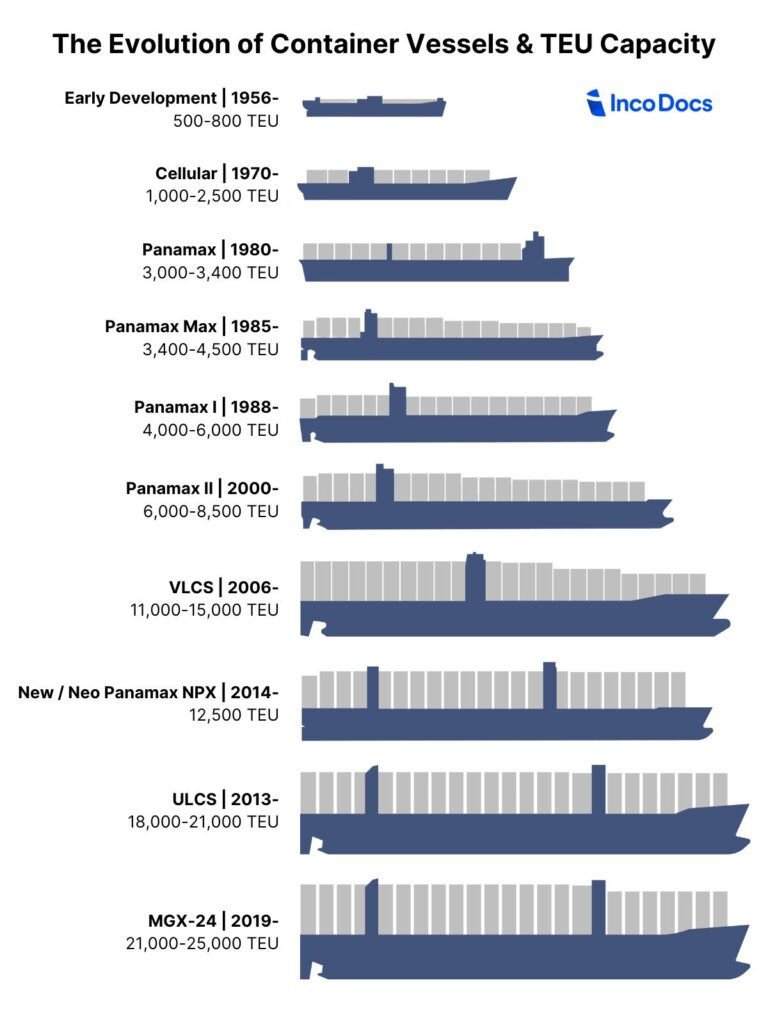
\includegraphics[width=0.5\textwidth,height=\textheight]{img/Gekle/Evolution-Container-Schiffe.jpg}
\caption{Entwicklung von Container Schiffen
{[}\protect\hyperlink{ref-IncoDocs-TEU}{76}{]}}
\end{figure}

Im Rahmen der Diplomarbeit werden aber nur 3 Prototypen angefertigt,
welche einerseits die benötigten Umweltdaten liefern, andererseits aber
auch miteinander kommunizieren. Die Komplexität eines
``Containergeflechts'' bestehend aus nur 3 Containern hält sich daher in
Grenzen und um den vollen Umfang unserer Diplomarbeit zu
veranschaulichen ist ein anderer Weg vonnöten. Dies ist, wo der
Simulator ins Spiel kommt: Er übernimmt die Aufgabe, ein System an
Containern ohne hunderten oder gar tausenden Prototypen darzustellen.

\hypertarget{graphentheorie}{%
\paragraph{Graphentheorie}\label{graphentheorie}}

Das Endergebnis des Simulators sollt ein Graph sein, welcher dabei
hilft, die Verbindungen zwischen den einzelnen Containern zu skizzieren.
Die Graphentheorie, ein Teilgebiet der Mathematik, spielt hierbei eine
essenzielle Rolle.

Allgemein gilt folgendes:

\begin{quote}
Ein \textbf{Graph} G besteht aus einer Menge V von \textbf{Knoten} und
einer Menge E von Knotenpaaren, welche als \textbf{Kanten} bezeichnet
werden. Die Notation für einen Graphen lautet G=(V,E)G=(V,E). E und V
stehen dabei für \emph{edges} und \emph{vertices}, also die englischen
Begriffe für Kanten und Knoten. Eine Kante \{u, v\} ELEMENT E verbindet
die Knoten u und v.
{[}\protect\hyperlink{ref-Uni-Bremen-Graphentheorie}{77}{]}
\end{quote}

Zusätzlich muss man innerhalb der Graphentheorie zwischen Ungerichteten
und Gerichteten Graphen unterscheiden. Der primäre Unterschied liegt
darin, ob die Kanten als einfache Striche (ungerichtet) oder Pfeile
(gerichtet) dargestellt werden.
{[}\protect\hyperlink{ref-Studyflix-Graphentheorie}{78}{]} Bei einem
gerichteten Graph ist daher die Richtung der Kante/ Beziehung zu
beachten. Gilt z.B. A -\textgreater{} B -\textgreater{} C mit V=\{A, B,
C\} und E=\{\{A,B\}, \{B,C\}\}, dann ist es nicht erlaubt, etwa von C zu
B zu gehen, sondern nur von B nach C. Bei einem ungerichteten Graph gilt
diese Regel nicht. Selbiges Beispiel nur ungerichtet: A - B - C; hier
darf man sowohl von B nach C als auch umgekehrt von C nach B gehen.

Abschließend muss man noch auf den Zusammenhang der einzelnen Knoten
schauen. Ein ungerichteter Graph ist dann zusammenhängend, wenn alle
Knoten erreichbar, also es zu jedem Knoten einen Weg gibt. Ist dies
nicht der Fall, gibt es sogenannte isolierte Knoten und der Graph ist
nicht zusammenhängend. Bei gerichteten Graphen unterscheidet man
zusätzlich zwischen schwach und stark zusammenhängenden Graphen.
{[}\protect\hyperlink{ref-Studyflix-Graphentheorie}{78}{]} In dem
Beispiel A -\textgreater{} B mit V=\{A, B\} und E=\{A,B\}, ist der
Knoten A nur erreichbar, wenn man die Richtung außer Acht lässt, man
spricht von einem schwach zusammenhängenden Graph. Für einen stark
zusammenhängenden Graph müsste zusätzlich noch eine Kante \{B, A\}
bestehen.

Der Containersimulator hat als Endergebnis einen \textbf{ungerichteten}
Graphen wie im folgenden Bild zu sehen ist:

\begin{figure}
\centering
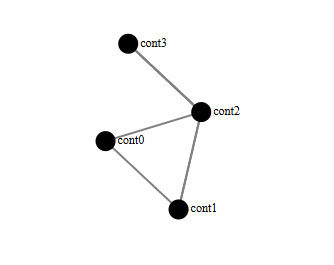
\includegraphics{img/Gekle/GraphExample.png}
\caption{Beispiel eines ungerichteten Graphen}
\end{figure}

Anhand des beispielhaften Graphs, lässt sich also folgendes herauslesen:

\begin{itemize}
\tightlist
\item
  Es gibt insgesamt 4 Knoten: V = \{con0, con1, con2, con3\}
\item
  Es gibt insgesamt 4 Kanten: E = \{\{cont0, cont1\}, \{cont0, cont2\},
  \{cont1, cont2\}, \{cont2, cont3\}\}
\end{itemize}

Die Beziehungen der Knoten im ungerichteten Graphen zueinander werden
mittels Adjazenzen und Inzidenzen beschrieben werden. Man spricht von
inzident, wenn bei einem Knoten V und einer Kante E folgendes gilt:
\(V \in E\). In anderen Worten: Eine Kante E verbindet den Knoten V mit
einem anderen Knoten im Graph. Zwei Knoten V und W sind miteinander
adjazent bzw. benachbart, falls mit einer Kante \(E \in {V, W}\) eine
direkte Verbindung zwischen den beiden Knoten existiert. Auch Kanten
können inzident sein, wenn sie beide zu einem gemeinsamen (benachbarten)
Knoten gehören.
{[}\protect\hyperlink{ref-Uni-Bremen-Graphentheorie}{77}{]}

\hypertarget{inzidenzmatrix}{%
\subparagraph{Inzidenzmatrix}\label{inzidenzmatrix}}

Unter einer Inzidenzmatrix versteht man eine n x m Matrix (n\ldots{}
Anzahl der Knoten V und m\ldots{} Anzahl der Kanten E). Durch die
Erstellung der Inzidenzmatrix lassen sich die Inzidenzen abbilden, also
man erkennt, ob der jeweilige Knoten an einer Kante anliegt oder nicht.
{[}\protect\hyperlink{ref-BWL-Lexikon-Inzidenzmatrix}{79}{]}

Als Beispiel eine Erweiterung des Graphs von oben:

\begin{figure}
\centering
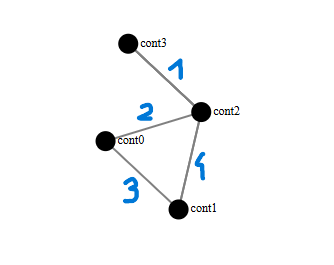
\includegraphics{img/Gekle/GraphExampleExtended.png}
\caption{Nummerierung der Kanten des obrigen Graphen}
\end{figure}

Hier wurden die Kanten durchnummeriert um die \textbf{Inzidenzmatrix} zu
erstellen:

\begin{longtable}[]{@{}lllll@{}}
\toprule
\textbf{V/ E} & \textbf{1} & \textbf{2} & \textbf{3} &
\textbf{4}\tabularnewline
\midrule
\endhead
\textbf{cont0} & 0 & 1 & 1 & 0\tabularnewline
\textbf{cont1} & 0 & 0 & 1 & 1\tabularnewline
\textbf{cont2} & 1 & 1 & 0 & 1\tabularnewline
\textbf{cont3} & 1 & 0 & 0 & 0\tabularnewline
\bottomrule
\end{longtable}

(1\ldots{} Verbindung; 0\ldots{} keine Verbindung) (V\ldots{} Knoten)
(E\ldots{} Kanten)

\hypertarget{adjazenzmatrix}{%
\subparagraph{Adjazenzmatrix}\label{adjazenzmatrix}}

Wie für Inzidenzen gibt es auch für Adjazenzen eine Matrix, hierbei
werden also die Nachbarschaften der einzelnen Knoten V abgebildet. Die
Matrix ist bei einer Anzahl N an Knoten V also n x m groß. Ein Vorteil
der Adjazenzmatrix ist, dass die Anzahl der Kanten E keine Rolle spielt
und sie sich somit sehr gut als Rechenbasis für rechnerische
Verarbeitungen des dazugehörigen Graphen eignet. Auch für die
Durchführung von Analysen eignet sie sich sehr gut, so kann die Matrix
etwa für folgendes hergezogen werden:

\begin{itemize}
\tightlist
\item
  Ermittlung erreichbarer Knoten
\item
  Errechnen von Pfadlängen
\item
  Analyse von Schleifenfreiheit
\end{itemize}

{[}\protect\hyperlink{ref-BigDataInsider}{80}{]}

Auch hier wird wieder das Beispiel aus dem Kapitel Indizenzmatrix
verwendet und so folgende Adjazenzmatrix erstellt:

\begin{longtable}[]{@{}lllll@{}}
\toprule
V/ W & cont0 & cont1 & cont2 & cont3\tabularnewline
\midrule
\endhead
\textbf{cont0} & \textbf{0} & 1 & 1 & 0\tabularnewline
\textbf{cont1} & 1 & \textbf{0} & 1 & 0\tabularnewline
\textbf{cont2} & 1 & 1 & \textbf{0} & 1\tabularnewline
\textbf{cont3} & 0 & 0 & 1 & \textbf{0}\tabularnewline
\bottomrule
\end{longtable}

(1\ldots{} Verbindung; 0\ldots{} keine Verbindung) (V\ldots{} Knoten)
(W\ldots{} 2. Knoten)

Wenn ein Knote V = Knote W ist, also bei einer Verbindung zu sich selbst
wird 0 eingetragen. Dadurch entsteht in jeder Adjazenzmatrix eines
ungerichteten Graph eine 0-Diagonale, welche oben auch gekennzeichnet
wurde.

\hypertarget{visualisierung-von-graphen}{%
\paragraph{Visualisierung von
Graphen}\label{visualisierung-von-graphen}}

\hypertarget{dot}{%
\subparagraph{DOT}\label{dot}}

Mithilfe der DOT Sprache, welche Teil von Graphviz
{[}\protect\hyperlink{ref-Graphviz-Homepage}{81}{]} ist, lassen sich
sehr einfach gerichtete und ungerichtete Graphen darstellen. Dies
erfolgt mit sogenannten ``edgeloops'', wobei ``-\textgreater{}'' für
gerichtete und ``--'' für ungerichtete Graphen steht. Diese können
innerhalb eines Graphen benutzt werden, welcher durch
\passthrough{\lstinline!graph\{\}!} für einen ungerichtete oder
\passthrough{\lstinline!diagraph\{\}!} für einen gerichteten
gekennzeichnet wird. Fügt man davor ein \passthrough{\lstinline!strict!}
hinzu (also z.B. \passthrough{\lstinline!strict graph\{\}!}) so kann man
bestimmen, dass zwischen zwei Knoten immer nur eine Verbindung besteht.
{[}\protect\hyperlink{ref-GraphViz-Documentation}{82}{]} Basierend auf
der Adjazenzmatrix kann man etwa so einen einfachen Graph erstellen:

\begin{lstlisting}[caption={Beispiel DOT Code}]
strict graph G {
    
  cont0 -- cont1;
  cont0 -- cont2;
  
  cont1 -- cont2;
  cont1 -- cont0;
  
  cont2 -- cont0;
  cont2 -- cont1;
  cont2 -- cont3;
  
  cont3 -- cont2;
}
\end{lstlisting}

Dieser Code würde folgendem entsprechen:

\begin{figure}
\centering
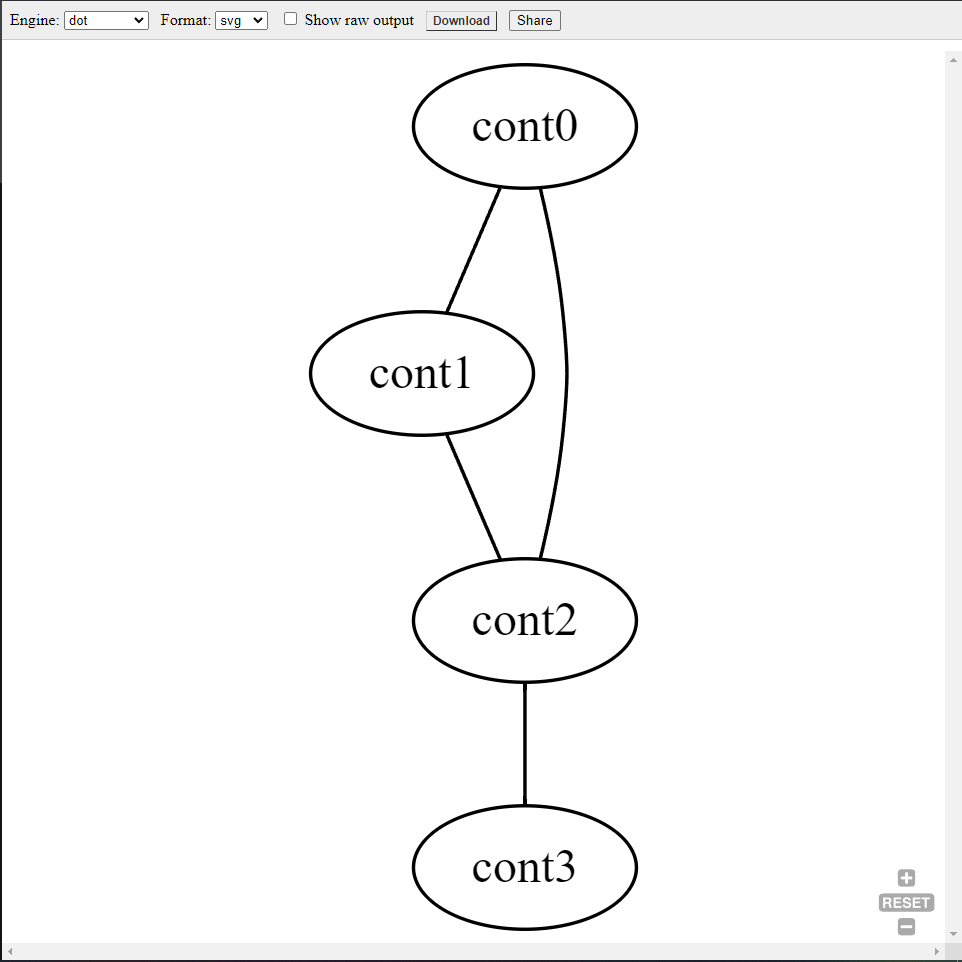
\includegraphics{img/Gekle/DotGraph.png}
\caption{Ungerichteter Graph mit DOT}
\end{figure}

\hypertarget{dragable-graph-dg}{%
\subparagraph{Dragable Graph (DG)}\label{dragable-graph-dg}}

Der große Vorteil des Dragable Graphs besteht darin, dass er interaktiv
ist. Ein User kann also mit dem Mauszeiger die einzelnen Knoten hin und
her bewegen, wobei auch die Kanten sich mit bewegen. Dies hilft
besonders bei der Benutzerfreundlichkeit, da sich der User den Graphen
so richten kann, wie es ihm gefällt, wodurch sie sich sehr gut für
Datenvisualisierung eignen. Eine JavaScript Bibliothek um so einem Graph
zu ermöglichen ist z.B. D3.js.
{[}\protect\hyperlink{ref-D3js-Homepage}{83}{]}, welcher auch in der
Diplomarbeit verwendet wurde.
{[}\protect\hyperlink{ref-gpt-DragableGraph}{84}{]} Des weiteren ist es
eine weitere Eigenschaft des DG, dass sich Knoten nicht übereinander
lagern können, da sie sich von einander abstoßen. Durch diese Mechanik
spannt sich der Graph automatisch auf und sorgt für eine übersichtliche
Visualisierung der Contaiener (Knoten), ohne dass sie sich gegenseitig
verdecken.

\hypertarget{website}{%
\subsubsection{Website}\label{website}}

\hypertarget{react}{%
\paragraph{React}\label{react}}

Bei React handelt es sich anders als bei z.B. Angular nicht tatsächlich
um ein Framework im herkömmlichen Sinne. Vielmehr ist es eine Bibliothek
zum Rendern graphischer Oberflächen. React setzt sehr stark auf
Komponentenorientierung, wobei zwischen klassenbasierten und
funktionalen Komponenten unterschieden wird. Die Tendenz geht allerdings
immer mehr in Richtung funktioneller Komponente.
{[}\protect\hyperlink{ref-Heise-React}{85}{]}

Auch hier im folgenden Beispiel ist eine funktionelle Komponente der
Diplomarbeits-Website zu sehen. Dies lässt sich u.a. an dem für
JavaScript typischen Syntax wie das ``=\textgreater{}'' erkennen, aber
auch daran, dass sogenannte Hooks (z.B. useStates) verwendet werden:

\begin{lstlisting}[caption={Beispiel funktionelle Komponente LoginField}]
const LoginField = ({ placeholder, value, onChange, isPassword = false }) => {
  const [showPassword, setShowPassword] = useState(false);
  const togglePasswordVisibility = () => {(...)}
  return (
    <div className="relative mb-4"> 
    (...)
    </div>
  );
};
export default LoginField;
\end{lstlisting}

\passthrough{\lstinline!LoginField!} kann rein theoretisch überall
eingesetzt werden, da diese Komponente an und für sich nur eine
spezielle Funktion übernimmt, jedoch kann man Komponenten aber auch so
gestalten, dass sie sich je nach Einsatzgebiet sich unterschiedlich
verhalten (z.B. anders aussehen, verschiedene andere Komponente
übernehmen etc.).

Im folgenden Code lässt sich dies auch gut erkennen. Der Code entspringt
einer ``Page'', also einer Seite, welche der User sieht. Der Code wird
aber nicht von oben bis unten durch in dieser einen Page (ebenfalls eine
funktionelle Komponente) geschrieben, sondern in mehrere Komponenten
aufgebrochen. Diese können dann ganz einfach in die Page eingefügt
werden. (z.B. \passthrough{\lstinline!Sidebar!},
\passthrough{\lstinline!Topbar!}, \passthrough{\lstinline!Detailspace!}
usw.). Betrachtet man die \passthrough{\lstinline!Topbar!} Komponente,
so sieht man, dass ihr weitere Komponenten übergeben werden, welche sie
dann nutzen kann. Wie eben erwähnt können die Parameter oder Komponenten
welche übergeben werden von Anwendungsfall zu Anwendungsfall komplett
unterschiedlich sein:

\begin{lstlisting}[caption={Unterschiedliche Verwendung von funktionelle Komponenten}]
<div className="flex h-screen">
  <Sidebar selectedShip={selectedShip} />
  <div className="flex-grow flex flex-col">
    <Topbar // Topbar in der MainPage
      leftComponents={[
        <SearchBar key="searchbar" selectedShip={selectedShip} onSearchSubmit=
        {handleSearchSubmit}
        />,
        <ShipSelect key="shipButton" ships={ships} selectedShip={selectedShip}
          onShipChange={setSelectedShip}
        />,
      ]}
      rightComponents={[
        <GridDropDown key="gridDropdown" gridSize={gridSize} setGridSize={setGridSize}
        />,
      ]}
    />
  </div>
</div>
\end{lstlisting}

Die \passthrough{\lstinline!Topbar!}-Komponente übernimmt in einer
anderen Page etwa ganz andere Komponenten wie hier zu sehen ist:

\begin{lstlisting}[caption={Alternative Verwendung der Topbar Komponente}]
// Topbar in der DetailPage
<Topbar
  leftComponents={[<SearchBar key="searchbar" />]}
  rightComponents={[
    <DetailControl
    onGoAlertClick={handleThreshholdViewerToggle} // Pass handler
  />
  ]}
/>
\end{lstlisting}

Anders als im ersten Code, wo eine \passthrough{\lstinline!Searchbar!}-,
\passthrough{\lstinline!ShipSelect!}- und
\passthrough{\lstinline!GridDropDown!}-Komponente übergeben wird, wird
hier etwa eine \passthrough{\lstinline!DetailControl!}-Komponente
übergeben. Die Funktionalität als auch das Aussehen der
\passthrough{\lstinline!Topbar!} ändert sich so. Dieses
Komponenten-basierte programmieren ist das Herz von React Development.

Die Komponente werden in React nicht in reinen Javascript geschrieben
sondern verwenden mit \textbf{JSX} eine erweiderte Form davon:

\begin{quote}
JSX ist eine Syntaxerweiterung für JavaScript, die es Ihnen erlaubt,
Komponenten und Elemente ohne großen Aufwand zu erzeugen. JSX nutzt eine
Schreibweise, die den Tags in HTML gleicht. Innerhalb von JSX können Sie
JavaScript-Ausdrücke in geschweiften Klammern einfügen und so
beispielsweise Werte oder das Ergebnis eines Funktionsaufrufs anzeigen.
\end{quote}

Schleifen erzeugen Sie normalerweise, indem Sie eine Datenstruktur,
meist ein Array, mit der map-Methode in eine JSX-Struktur umwandeln.
Bedingungen mit if-Statements innerhalb der JSX-Strukturen zu
formulieren, ist nicht möglich.

Sie können dies entweder auslagern oder beispielsweise mit dem Ternär-
oder dem logischen Und-Operator arbeiten. {[}Buchquelle{]}

\hypertarget{use-state-hooks}{%
\subparagraph{Use-State \& Hooks}\label{use-state-hooks}}

\begin{quote}
Die Hooks-API stellt eine Aufwertung der Funktionskomponenten dar. Vor
der Einführung der neuen Schnittstelle war es nur in Klassenkomponenten
möglich, einen lokalen State zu implementieren und auf
Lifecycle-Methoden zurückzugreifen. Diese und weitere Einschränkungen
werden durch die Hooks weitestgehend aufgehoben. {[}Buchquelle{]}
\end{quote}

Die großen Vorteile, welche die Hooks mit sich bringen sind hierbei
folgende:

\begin{itemize}
\tightlist
\item
  Reduzierung des Komponentenumfangs
\item
  Entfernen von Duplikaten
\item
  Ersatz von komplexen Entwurfsmustern {[}Buchquelle{]}
\end{itemize}

Der \passthrough{\lstinline!useState!}-Hook erlaubt es nun aber, dass
State zu den funktionellen Komponenten hinzugefügt wird.
{[}\protect\hyperlink{ref-GeeksForGeeks-useState}{86}{]} Es können auch
mehrere State-Variablen in einer Komponente definiert werden. Ein
\passthrough{\lstinline!useState!} sieht in der Regel in etwa so aus:

\begin{lstlisting}[caption={Beispiel useState Variable}]
const [username, setUsername] = useState('User');
\end{lstlisting}

\begin{itemize}
\tightlist
\item
  username = aktueller Zustand
\item
  setUsername = Funktion um den Zustand zu aktualisieren
\item
  `User' = Anfangswert
\end{itemize}

Mit ``Hooks'' kann man sich also in die jeweilige Variable
``einklinken''.

Es gibt in React neben der useState auch noch andere Hooks. React selbst
unterteilt diese in ihrer Dokumentation wiefolgt:

\begin{itemize}
\tightlist
\item
  Basic Hooks
\item
  Additional Hooks
\item
  Library Hooks
\end{itemize}

Die 3 ``Basic Hooks'' sind hierbei allerdings die wichtigsten. Neben dem
bereits erwähnten \passthrough{\lstinline!useState()!} gibt es auch
noch:

\begin{itemize}
\tightlist
\item
  \passthrough{\lstinline!useEffect()!} --\textgreater{} für Ausführung
  von Side-Effects wie das Laden von Daten via API, Event-Handler oder
  die Konsolen Ausgabe
\item
  \passthrough{\lstinline!useContext()!} --\textgreater{} ermöglicht es
  Daten aus einem Context-Provider zu konsumieren
  {[}\protect\hyperlink{ref-DoubleSlash-ReactHooks}{87}{]}
\end{itemize}

\hypertarget{react-router}{%
\subparagraph{React Router}\label{react-router}}

Viele Webanwendungen sind sogenannte ``Single-Page-Webanwendungen''. Sie
bestehen also aus nur einem HTML-Dokument, wobei der Inhalt dynamisch
nachgeladen wird. Sogenannte SPA (Single Page Applications) beinhalten
also Komponenten, welche sich wie Seiten verhalten. Um so etwas zu
erstellen, muss React-Router und das Routing verwendet werden. Mithilfe
des Routings werden Komponenten Routen zugeordnet. Dies stellt
\passthrough{\lstinline!react-router-dom!} zur Verfügung
{[}\protect\hyperlink{ref-FreeCodeCamp-Routing}{88}{]}

Dies erfolgt über das ``Route'' Element:

\begin{lstlisting}[caption={Beispiel Route Element}]
<Route path="/main" element={<MainPage />} />
\end{lstlisting}

Hierbei wird über die URL ``\ldots/main'' auf die MainPage verwiesen.
Gibt man in der Adresszeile eines Browsers die URL ein, würde man rein
theoretisch auf der MainPage landen.

Es ist wichtig anzumerken, dass alle Routes logischerweise Teil eines
Routers sein müssen. Dies würde in etwa so aussehen:

\begin{lstlisting}[caption={Beispiel React Router}]
const router = createBrowserRouter(
  createRoutesFromElements(
    <>
    {/* Hier kommen die Routes hin */}
    </>
  )
);
\end{lstlisting}

\hypertarget{frontend-build-tool---vite}{%
\paragraph{Frontend Build Tool -
Vite}\label{frontend-build-tool---vite}}

Bei der Verwendung von React ist es empfehlenswert ein sogenanntes Build
Tool zu verwenden. Dieses übernimmt die Aufgabe des ``Building'',
worunter man den Prozess versteht, in welchem der eigene Source Code so
transformiert und gebündelt wird, dass er von Browsern interpretiert
werden kann. {[}\protect\hyperlink{ref-CodeParrot-BuildTools}{89}{]}

Die zentralen Aufgaben eines Build Tools sind:

\begin{itemize}
\tightlist
\item
  konvertieren des JavaScript/ TypeScript Codes in eine für Browser
  kompatible Version
\item
  bündeln von Komponenten und Files um die Anzahl an HTTP Requests für
  das Laden der App zu verringern
\item
  unnütze Zeichen (z.B. Whitespaces) löschen um Ladezeiten zu verbessern
\item
  allgemein die Performance des Codes verbessern (z.B. mit ``Tree
  Shaking'', welches unbenutzten Code
  eliminiert){[}\protect\hyperlink{ref-CodeParrot-BuildTools}{89}{]}
\end{itemize}

Eines dieser Build Tools ist Vite, welches sich besonders durch seine
Geschwindigkeit auszeichnet (vite = französisch für schnell). Zu den
Gründen warum Vite mittlerweile so beliebt ist zählen u.a.:

\begin{itemize}
\tightlist
\item
  Geschwindigkeit --\textgreater{} benutzt ES, um Quellcode direkt im
  Browser bereitzustellen
\item
  out-of-the-box Support für React/TypeScript/\ldots{}
\item
  optimierter Build durch die Verwendung von Rollup als Bundler
  {[}\protect\hyperlink{ref-CodeParrot-BuildTools}{89}{]}
\end{itemize}

\begin{figure}
\centering

\includegraphics[width=1\textwidth,height=\textheight]{img/Gekle/Vite-Features.png}
\caption{Funktionen von Vite
\protect\hyperlink{ref-eluminoustechnologies-vite}{90}}
\end{figure}

Selbst aber mit dem sogenannten HMR (Hot Module Replacement
--\textgreater{} Änderungen im Code werden sofort im Browser angezeigt)
tendieren Build Tools dazu, mit wachsendem JavaScript langsamer zu
werden. Hierbei ist Vite jedoch besonders. Es nutzt eine Kombination aus
ES Modulen und einem virtuellen Modulsystem:
{[}\protect\hyperlink{ref-Telerik-BuildTools}{91}{]}

\begin{quote}
Wenn Sie ein Modul importieren, behandelt Vite es als virtuelles Modul.
Während der Entwicklung bündelt es nicht Ihren gesamten Code in eine
einzelne Datei. Stattdessen erstellt es bei Bedarf Builds für jedes
Modul und stellt sie in separaten Dateien bereit. Dieser Ansatz
eliminiert die Notwendigkeit eines vollständigen Bündelungsprozesses bei
jeder Änderung, führt zu schnelleren Reloads und -- natürlich -- zu
einem zufriedenen Entwickler.
{[}\protect\hyperlink{ref-Telerik-BuildTools}{91}{]}
\end{quote}

\hypertarget{erstellen-aufbau-eines-vite-react-projekt}{%
\subparagraph{Erstellen \& Aufbau eines Vite
React-Projekt}\label{erstellen-aufbau-eines-vite-react-projekt}}

Unter der Annahme, dass \passthrough{\lstinline!Node.js!} installiert
ist, ist es sehr einfach, ein React Projekt mithilfe von Vite zu
erstellen. Hierfür muss man einfach innerhalb eines Terminals folgenden
Befehl ausführen:

\begin{lstlisting}[caption={Befehl zum Erstellen eines React-Projekts mit Vite}]
npm create vite@latest project-name
\end{lstlisting}

{[}\protect\hyperlink{ref-React-CrashCourse}{92}{]}

Mithilfe diesen Befehls wird der Prozess zum Erstellen eines neuen React
Projekts mit der neuesten Vite Version gestartet. Als erstes wird
folgendes gefragt:

\begin{figure}
\centering
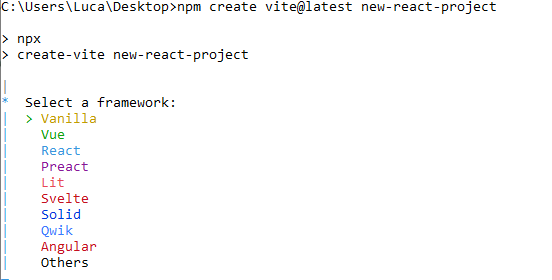
\includegraphics[width=0.75\textwidth,height=\textheight]{img/Gekle/CreateProject1.png}
\caption{Auswahl des Projekttyps nach npm Befehl}
\end{figure}

Um ein React Project speziell zu erstellen muss natürlich ``React''
mithilfe der Pfeiltasten und Enter ausgewählt werden. Daraufhin wird
noch gefragt, ob man Typescript oder JavaScript verwenden möchte (siehe
Bild unten). Im Rahmen der Diplomarbeit wurde einfach nur JavaScript
ausgewählt.

\begin{figure}
\centering
\includegraphics[width=0.75\textwidth,height=\textheight]{img/Gekle/CreateProject2.png}
\caption{Auswahl zwischen TypeScript und Javascript während der
Projekterstellung}
\end{figure}

Ist dies einmal gemacht, kann das Projekt mithilfe eines Code-Editors
geöffnet werden. Innerhalb des Projekts kann dann ein
\passthrough{\lstinline!vite.config.js!}-File gefunden werden, in
welchen man die Konfigurationen des Projekts (etwa den Port) ändern
kann. Um aber alles funktional zu machen müssen mit
\passthrough{\lstinline!npm install!} noch die Dependencies installiert
werden. In einem regulären Projekt würde man dann mit dem Befehl
\passthrough{\lstinline!npm run dev!} das React-Projekt starten. Bei
jedem React-Projekt handelt es sich wie bereits erwähnt um eine
``Single-Page-Application''. Diese ``Single-Page'' bildet
\passthrough{\lstinline!index.html!}, und alles weitere (Komponente)
werden via JavaScript dazugeladen. Als Einstiegsfile dient die
sogenannte \passthrough{\lstinline!main.jsx!}, welche (standardmäßig)
\passthrough{\lstinline!app.jsx!} lädt, welche wiederum die
Hauptkomponente des Projekts bildet.
{[}\protect\hyperlink{ref-React-CrashCourse}{92}{]}

\begin{lstlisting}[language=HTML, caption={index.html File}]
<!doctype html>
<html lang="en">
  <head>
    <meta charset="UTF-8" />
    <link rel="icon" type="image/svg+xml" href="/src/img/LogoSimple.png" />
    <meta name="viewport" content="width=device-width, initial-scale=1.0" />
    <title>Contrude</title>
  </head>
  <body>
    <div id="root"></div>
    <script type="module" src="/src/main.jsx"></script>
  </body>
</html>
\end{lstlisting}

Generell gibt es regulär 2 CSS-Files, da jedoch TailwindCSS benutzt
wird, wird nur eines davon benötigt:
\passthrough{\lstinline!index.css!}. Um TailwindCSS (Version 3.4) zu
installieren müssen nach dem React-Projekt Erstellen selbst noch
folgende 2 Befehle im Terminal ausgeführt werden:

\begin{lstlisting}[caption={TailwindCSS Installieren Befehle}]
npm install -D tailwindcss@3 postcss autoprefixer
npx tailwindcss init -p
\end{lstlisting}

{[}\protect\hyperlink{ref-TailwindCSS-Docs-ViteSetup}{93}{]}

Danach müsssen über die neu erschienene
\passthrough{\lstinline!tailwind.config.js!} noch die Pfade definiert
werden und der Inhalt der \passthrough{\lstinline!index.css!} mit
folgendem ersetzt werden:

\begin{lstlisting}[caption={Updaten der index.css für TailwindCSS}]
@tailwind base;
@tailwind components;
@tailwind utilities;
\end{lstlisting}

{[}\protect\hyperlink{ref-TailwindCSS-Docs-ViteSetup}{93}{]}

Ist dies gemacht, kann TailwindCSS innerhalb des (gesamnten) Projekts
genutzt werden.

\hypertarget{tailwind-css}{%
\paragraph{Tailwind CSS}\label{tailwind-css}}

Tailwind CSS ist ein CSS Framework, welches darauf abzielt das Designen
von Webanwendungen zu vereinfachen, indem vordefinierte Utility Klassen
benutzt werden.
{[}\protect\hyperlink{ref-GeeksForGeeks-TailwindCSS}{94}{]}

Der Unterschied zwischen Tailwind CSS und traditionellen CSS könnte z.B.
so aussehen (in React): Ohne Tailwind CSS:

\begin{lstlisting}[language=HTML, caption={Div in HTML}]
<div class="search-container"> CODE </div>
\end{lstlisting}

\begin{lstlisting}[caption={Traditionelles CSS für das obige Div}]
.search-container {
    width: 18rem; /* w-72 */
    padding-left: 0.75rem; /* pl-3 */
    height: 2.25rem; /* h-9 */
    background-color: white;
    display: flex;
    justify-content: flex-start;
    align-items: center;
    border: 2px solid black;
    border-top-left-radius: 9999px; /* rounded-l-full */
}
\end{lstlisting}

Mit Tailwind CSS:

\begin{lstlisting}[caption={CSS styling eines Div mit Tailwind}]
<div className='w-72 pl-3 h-9 bg-white flex justify-start items-center border-2 border-black rounded-l-full'>
  CODE
</div>
\end{lstlisting}

Tailwind CSS scannt alle HTML-Dateien, JavaScript-Komponenten und andere
Templates nach Klassenbezeichnern. Diese Bezeichner, die im Code
verwendet werden (z. B. \passthrough{\lstinline!w-72!},
\passthrough{\lstinline!bg-white!}, \passthrough{\lstinline!flex!}),
repräsentieren bestimmte Stileigenschaften. Nachdem Tailwind alle
genutzten Klassen gefunden hat, generiert es die entsprechenden
CSS-Regeln und schreibt sie in eine statische CSS-Datei.
{[}\protect\hyperlink{ref-TailwindCSS-Docs-GettingStarted}{95}{]}

Es ist auch möglich, Tailwind CSS mit bestimmten Ereignissen zu
verknüpfen. So ist es z.B. möglich folgendes zu tun:

\begin{lstlisting}[caption={Hover Funktion von Tailwind CSS}]
<button className='bg-red-400 hover:bg-red-600'>BUTTON</button>
\end{lstlisting}

Dies sagt aus, dass im Zustand ``hover'', also wenn der User mit dem
Mauszeiger über den Knopf hovert, der Farbton von
\passthrough{\lstinline!red-400!} auf den dunkleren Rotton
\passthrough{\lstinline!red-600!} geändert werden soll. Bezüglich den
Farben bietet TailwindCSS allgemein eine sehr große Palette an
vordefinierten Farben, welche mit Texten, Border-Liniern oder auch dem
eben erwähnten \passthrough{\lstinline!hover!} kombiniert werden können.
Dies lässt sich auch im Bild sehr gut erkennen:

\begin{figure}
\centering
\includegraphics{img/Gekle/TailwindCSS-Colors-Example.PNG}
\caption{Vordefinierte Farben von TailwindCSS}
\end{figure}

Tailwind nennt dies Pseudo Klassen. Die 3 wichtigsten sind folgende:

\begin{itemize}
\tightlist
\item
  Hover --\textgreater{} aktiviert, wenn der User über das Element
  hovert
\item
  Focus --\textgreater{} aktiviert, wenn der User das Element z.B. durch
  einen Klick in Fokus nimmt
\item
  Active --\textgreater{} aktiviert, wenn der User das Element durch
  User aktiviert wird
  {[}\protect\hyperlink{ref-TailwindCSS-DocsV1}{96}{]}
\end{itemize}

All diese Pseudo Klassen können auch mit ``group-'' verbunden werden, um
mehrere Code-Teile gleichzeitig zu manipulieren.
{[}\protect\hyperlink{ref-TailwindCSS-DocsV1}{96}{]}

Die großen Vorteile von Tailwind CSS sind also, dass keine externen CSS
Files erstellt werden müssen und man sich nicht immer komplexere
Klassen-Namen ausdenken muss. Auch die eingebaute Reaktionsfähigkeit
spricht für das Framework. Zusätzlich bietet Tailwind eine umfassende
Dokumentation, was das programmieren viel einfacher und effizienter
macht. {[}\protect\hyperlink{ref-GeeksForGeeks-TailwindCSS}{94}{]}

\hypertarget{rest-und-axios}{%
\paragraph{REST und Axios}\label{rest-und-axios}}

Die Webanwendung benötigt, damit sie ordentlich und sinnvoll
funktioniert Daten aus dem Backend. Diese Daten werden über die REST
(Representational State Transfer) API in das Frontend (sprich die
Website) geholt.

\hypertarget{rest}{%
\subparagraph{REST}\label{rest}}

Die API, welche aufgrund ihrer Flexibilität, Schnelligkeit und
Einfachheit berühmt wurde benutzt in der Regel das HTTP-Protokoll und
überträgt die Daten mithilfe von JSON. Im Kontext einer Website wird mit
dem Eingeben/Aufrufen einer URL, eine HTTP Anfrage gesendet. Die
wichtigsten HTTP Befehle hierbei sind:

\begin{itemize}
\tightlist
\item
  GET (Abrufen)
\item
  POST (Erstellen)
\item
  PUT (Aktualisieren)
\item
  DELETE (Löschen) {[}\protect\hyperlink{ref-Talend-REST}{97}{]}
\end{itemize}

Die Anfrage geht dann beim Server ein und die REST API kümmert sich
darum, dass eine Antwort gesucht und sofort zurückgeliefert wird. Die
Antworten sind in der Regel im JSON (JavaScript Object Notation) Format.
{[}\protect\hyperlink{ref-Talend-REST}{97}{]}

\hypertarget{kriterien-fuxfcr-rest}{%
\subparagraph{Kriterien für REST}\label{kriterien-fuxfcr-rest}}

Damit eine REST API gültig ist, müssen 6 Kriterien erfüllt sein:

\begin{enumerate}
\def\labelenumi{\arabic{enumi}.}
\tightlist
\item
  Architektur --\textgreater{} Clients, Servern und Ressourcen bei
  welcher Anfragen über HTTP laufen
\item
  ``Statelessness'' --\textgreater{} es werden keine
  Client-Informationen zwischen Anfragen gespeichert
\item
  Cachefähige Daten --\textgreater{} optimiert Interaktion zwischen
  Client und Server
\item
  einheitliche Schnittstelle zwischen Komponenten --\textgreater{} von
  überall kann auf Ressourcen gleich zugegriffen werden
\item
  mehrschichtiges System --\textgreater{} organisiert einzelne
  Servertypen und macht Struktur für Client unsichtbar
\item
  Code-On-Dmand --\textgreater{} auf Anforderungen ausführbaren Code von
  Server an Client senden (optional)
  {[}\protect\hyperlink{ref-RedHat-REST}{98}{]}
\end{enumerate}

\hypertarget{rest-in-react---axios}{%
\subparagraph{REST in REACT - Axios}\label{rest-in-react---axios}}

Es ist durchaus möglich, HTTP Abfragen innerhalb von React ohne externer
Library zu benutzen. Allerdings hat eine benutzerfreundliche externe API
wie Axios durchaus seine Vorteile. Axios verwendet Promises (JavaScript
Objekte welche den zukünftigen Wert einer asynchronen Funktion
repräsentiert), wodurch es einfacher ist mit ``asnyc functions'' zu
arbeiten. Auch die Tatsache, dass Axios automatisch JSON Objekte in
JavaScript Objekte überführt, sprich man ersparrt sich die
\passthrough{\lstinline!.json!}-Anweisung, spricht für die Verwendung
davon. Zusätzliche Vorteile von Axios sind:

\begin{itemize}
\tightlist
\item
  eingebaute Funktionen zum Abbrechen von Abfragen
\item
  interzeptieren (vor Senden einer Abfrage/ nach Erhalten einer Antwort
  logische Operationen durchführen)
\item
  hat CSRF (Cross Site Request Forgery) Schutz
\item
  breite Community + Support
  {[}\protect\hyperlink{ref-GeeksForGeeks-Axios}{99}{]}
\end{itemize}

Weiters ist der Code mit Axios etwas einfacher zu lesen: Ohne:

\begin{lstlisting}[caption={Beispiel REST Call mit fetch-api}]
const response = await fetch('https://api.contrude.eu/login', { 
  method: 'POST', 
  headers: { 'Content-Type': 'application/json', }, 
  body: JSON.stringify(loginData), });
\end{lstlisting}

Mit:

\begin{lstlisting}[caption={Beispiel REST Call mit Axios}]
const response = await axios.post('https://api.contrude.eu/login', loginData, { 
headers: { 'Content-Type': 'application/json', }, });
\end{lstlisting}

Die BaseURL und der Header sind bei jedem Call über die gesamte Website
hinweg die gleichen, daher kann man in einem separaten JavaScript File
eine sogenannte Axios Instanz
{[}\protect\hyperlink{ref-gpt-AxiosVT}{100}{]} erstellen:

\begin{lstlisting}[caption={Axios Instanz}]
import axios from 'axios';

const axiosInstance = axios.create({
  baseURL: 'https://api.contrude.eu',
  headers: {
    'Content-Type': 'application/json',
  },
});

export default axiosInstance;
\end{lstlisting}

{[}\protect\hyperlink{ref-Axios-Docs-Instance}{101}{]}

Diese wird dann in allen Komponenten eingebunden, in welchen man
REST-Abfrage durchführt:
\passthrough{\lstinline!import axiosInstance from '../api/AxiosInstance';!}

Ein Call würde dann noch vereinfachter aussehen:

\begin{lstlisting}[caption={Beispiel REST Call mit Axios + Instanz}]
const response = await axiosinstance.post('https://api.contrude.eu/login', loginData);
\end{lstlisting}

Die Fehlerbehandlung ist durch Axios ebenfalls verbessert. So sieht
fetch das Promise bei z.B. HTTP Fehlercodes wie 404 oder 500 trotzdem
als erfüllt. Sprich: Der Status Code muss explizit überprüft werden. Ein
Fehler wird also nur ausgelöst, wenn es sich um ein Netzwerkproblem
handelt (z.B. Server nicht erreichbar). Axios sieht HTTP-Fehler aber
automatisch als das, was sie sind, Fehler, und lehnt das Promise ab
wodurch die Fehlerbehandlung vereinfacht wird.
{[}\protect\hyperlink{ref-gpt-AxiosVT}{100}{]}

Alle Abfragen werden innerhalb von asynchronen Funktionen durchgeführt.
Dies hat einerseits den Vorteil, dass der Code besser lesbar ist, da
ohne \passthrough{\lstinline!async!} mit \passthrough{\lstinline!.then!}
und \passthrough{\lstinline!.catch!} gearbeitet werden muss. So wird
auch sogenannten ``Callback-Hells'' vorgebeugt, da man sich nicht in
\passthrough{\lstinline!then!} Schleifen verlieren kann. Auch die
Fehlerbehandlung ist aufgrund von \passthrough{\lstinline!try/catch!}
einfacher und sauberer.
{[}\protect\hyperlink{ref-gpt-WarumAsync}{102}{]}

\hypertarget{praktische-arbeit-2}{%
\subsection{Praktische Arbeit}\label{praktische-arbeit-2}}

\hypertarget{java-container-simulator-1}{%
\subsubsection{Java Container
Simulator}\label{java-container-simulator-1}}

\hypertarget{klassen}{%
\paragraph{Klassen}\label{klassen}}

\hypertarget{container-1}{%
\subparagraph{Container}\label{container-1}}

Diese Klasse ist eine etwas modifizierte POJO (Plain Old Java Object)
Klasse mit folgenden Variablen:

\begin{itemize}
\tightlist
\item
  String \passthrough{\lstinline!name!}
\item
  List\textless Container\textgreater{}
  \passthrough{\lstinline!adjacentContainers!}(ArrayList)
\item
  double \passthrough{\lstinline!signalMinimum!}
\end{itemize}

Die \passthrough{\lstinline!name!}-Variable aller Container ist gleich
aufgebaut: ``cont\#'', wobei \# für eine beliebige Nummer steht. Dies
macht die Namen nicht unnötig kompliziert und hat auch innerhalb der
Konsolen-Interaktion mit dem User seinen Vorteil. In
\passthrough{\lstinline!adjacentContainers!} werden alle benachbarten
Container, also jene, zu welchen der ausgewählte Container eine
Verbindung hat bzw. welche in seiner Nähe sind, abgespeichert. Die
Variable \passthrough{\lstinline!signalMinimum!} ist eine mithilfe von
\passthrough{\lstinline!ThreadLocalRandom.current()!} erstellte
zufällige Double-Variable, welche für das Generieren der Verbindung
zwischen den einzelnen Containern noch wichtig wird.
\passthrough{\lstinline!ThreadLocalRandom!} wird eigentlich eher für
Multithreading-Anwendungen benutzt
{[}\protect\hyperlink{ref-Baeldung-JavaRandom}{103}{]}, jedoch ist die
Syntax, um eine Zufallszahl mit ``von-bis'' zu generieren, etwas
angenehmer zu lesen:

\begin{lstlisting}[language=Java, caption={Zufällige Nummer mit .math und ThreadLocalRandom}]
// Mit Math.random
this.signalMinimum = 10 + (25 - 10) * Math.random();

// Mit ThreadLocalRandom
this.signalMinimum = ThreadLocalRandom.current().nextDouble(10, 25);
\end{lstlisting}

Der Grund hierfür ist, da \passthrough{\lstinline!Math.random!} nur eine
Zahl zwischen 0 \& 1 generiert, während man bei
\passthrough{\lstinline!ThreadLocalRandom!} den minimalen und maximalen
Wert einfach angeben kann.

Bezüglich Methoden hat \passthrough{\lstinline!Container!} für alle
Variablen Getter und Setter und einen Konstruktor, mit welchem
\passthrough{\lstinline!name!} und
\passthrough{\lstinline!signalMinimum!} gesetzt werden. Mithilfe von
\passthrough{\lstinline!void addDestination(Container con)!} kann ein
benachbarter Container zur Liste hinzugefügt werden (die Liste wird
außerhalb des Konstruktors initialisiert. Auch die
\passthrough{\lstinline!toString!} wurde etwas angepasst, um die Ausgabe
in der Konsole etwas besser aussehen zu lassen:

\begin{lstlisting}[language=Java, caption={Überarbeitung der .toString Methode von Container}]
@Override
public String toString() {
    StringBuilder adjacent = new StringBuilder();
    for (Container container : adjacentContainers) {
        adjacent.append(container.getName()).append(", ");
    }
  
    return "Container{" +
            "name='" + name + '\'' +
            ", adjacentContainers=" + adjacent +
            ", signalMinimum=" + signalMinimum +
            '}';
}
\end{lstlisting}

Entspricht:

\begin{lstlisting}[caption={Ausgabe mittels toString von Container}]
Container{name='cont1', adjacentContainers=cont0, , signalMinimum=10.753991237010691}
\end{lstlisting}

\hypertarget{ship}{%
\subparagraph{Ship}\label{ship}}

Dies ist die zweite Klasse, in welcher alle für den Simulator
notwendigen Funktionen implementiert sind. Die Klasse selbst verwaltet
drei Variablen:

\begin{itemize}
\tightlist
\item
  Set\textless Container\textgreater{}
  \passthrough{\lstinline!containers!} (HashSet)
\item
  ArrayList\textless String\textgreater{}
  \passthrough{\lstinline!contConList!}
\item
  int{[}{]}{[}{]} \passthrough{\lstinline!adjMatrix!}
\end{itemize}

In dem HashSet werden alle in der Main Klasse generierten Container
abgespeichert. In der \passthrough{\lstinline!contConList!} werden alle
Verbindungen zwischen Containern im Format ``A;B'' abgespeichert, wobei
A für Container (= Knoten im Graphen) und das Semikolon für die
Verbindung (=Kante im Graphen) stehen. Das 2d-Array repräsentiert eine
Adjazenzmatrix, welche u.a. für das Schreiben in JSON Files benötigt
wird.

Mit \passthrough{\lstinline!void addContainer (Container con)!} können
Container in das Set hinzugefügt werden. Weitere Methoden sind
diejenigen zum Schreiben in JSON Files oder jene, welche für das
Konsolen-Programm benötigt werden (z.B.
\passthrough{\lstinline!printAdjMatrix!} zum Schreiben der Adjazenz
Matrix). Außerdem erledigt sie die Aufgabe der Erstellung der
Verbindungen zwischen den einzelnen Container-Objekten.

\hypertarget{main}{%
\subparagraph{Main}\label{main}}

Der Container Simulator ist an und für sich ein Konsolen-Programm. Die
Interaktion zwischen dem User und dem Simulator passiert also (fast)
rein in der Konsole. Die \passthrough{\lstinline!Main!}-Klasse regelt
diese. Sie erstellt die Container, basierend auf der vom User
eingegebenen Menge, und übergibt diese an die ebenfalls von ihr
erstellten \passthrough{\lstinline!Ship!}-Klasse. Die User-Interaktion
wird dann innerhalb einer \passthrough{\lstinline!while!}-Schleife
fortgesetzt. Hier kann der User mehrere Buchstaben eingeben, welche für
verschiedene Aktionen stehen:

\begin{lstlisting}[language=Java, caption={Auswahlmöglichkeiten des Simulators}]
System.out.println("\nChoose an option:\n" +
        "(a) View single Container\n" +
        "(b) View Matrix\n" +
        "(c) Print Connection List\n" +
        "(d) Export to Json Format (all Containers)\n" +
        "(e) Export to Json Format (specific Container)\n" +
        "(q) Quit Simulator");
in = sc.nextLine();
\end{lstlisting}

Über einen \passthrough{\lstinline!Scanner!} wird diese Eingabe dann
geprüft. Das Ausführen der passenden Aktionen regelt ein
\passthrough{\lstinline!switch-case!}, wobei auf ein
\passthrough{\lstinline!default!} gesetzt ist, sollte die User-Eingabe
inkorrekt sein. Sobald der User ``q'' eingibt, bricht die
\passthrough{\lstinline!while!}-Schleife ab, dies wird durch folgenden
Ausdruck ermöglich:

\begin{lstlisting}[language=Java, caption={While Schleife in welcher die Main läuft}]
while(!in.equals("q")){}
\end{lstlisting}

\hypertarget{wie-die-dummy-daten-verbindungen-generiert-werden}{%
\paragraph{Wie die Dummy-Daten + Verbindungen generiert
werden}\label{wie-die-dummy-daten-verbindungen-generiert-werden}}

Startet man das Programm, so wird man als Erstes zu folgendem
aufgefordert:

\begin{figure}
\centering
\includegraphics{img/Gekle/SimulatorConsole1.png}
\caption{Anfangs-Konsolenausgabe des Simulators}
\end{figure}

Der User bestimmt also, wie viele Container für die Simulation erstellt
werden sollen. ``\textgreater=2'' wurde deshalb als Bedingung
eingeführt, da ein simuliertes Schiff mit nur einem Container keinem
Graph mit Knoten und Kanten entsprechen würde. Da es ja das Ziel ist,
die Kommunikationsstruktur mit Kanten darzustellen, macht die Auswahl 1
wenig Sinn.

Bestätigt der User seine Eingabe mit Enter, so wird ein
\passthrough{\lstinline!Ship!} Objekt erstellt. Dieses hat als zentrale
Variable ein \passthrough{\lstinline!Container!}-Set namens
\passthrough{\lstinline!containers!}, worin alle Container gespeichert
werden. Das Erstellen und Speichern der Container selbst passiert in der
\passthrough{\lstinline!Main!} mit folgendem Code:

\begin{lstlisting}[language=Java, caption={Code zum Erstellen der Container}]
for(int i = 0; i < count; i++){
    String containerName = "cont" + i;
    ship.addContainer(new Container(containerName));
}
\end{lstlisting}

Die \passthrough{\lstinline!count!} Variable ist zu Beginn auf -1
gesetzt. Dies hat den Hintergrund, da die Namen der Container bei 0
anfangen (also mit ``cont0''), der User aber die tatsächliche Anzahl
eingeben soll (z.B.: Eingabe = 7 --\textgreater{} Container Namen: cont0
bis cont6 = 7 Stk). Wichtig ist auch anzumerken, dass nur der Container
Name in \passthrough{\lstinline!ship!} gespeichert wird, da
\passthrough{\lstinline!signalMinimum!} einfach dann von den Methoden
selbst geholt wird, welche diese brauchen.

Nachdem die Container erstellt sind, müssen noch die Verbindungen bzw.
Nachbarschaften der Container bestimmt werden. Dies übernimmt folgende
Methode:

\begin{lstlisting}[language=Java, caption={Methode welche die Verbindungen zwischen einzelnen Containern erstellt}]
public void sendSetSignals(Container container){
    double signal = 15;
    double randomNum = ThreadLocalRandom.current().nextDouble(0.1, 1.0);
    boolean add = ThreadLocalRandom.current().nextBoolean();
  
    if(add){
        signal = signal + randomNum;
    }else{
        signal = signal - randomNum;
    }
  
    Container origin = container;
    for(Container cont : this.containers){
        if(!cont.getName().equals(origin.getName())){
            if(cont.getSignalMinimum() <= signal && checkContConList(origin.getName(),
             cont.getName())){
                origin.addDestination(cont);
                contConList.add(extractId(origin.getName()) + ";" +
                extractId(cont.getName()));
            }
        }
    }
    redoAllMinSignals();
}
\end{lstlisting}

Als Basis-Signal wurde willkürlich 15 hergenommen, dieser Wert wird dann
um einen zufälligen Wert zwischen 0.1 und 1 ebenfalls zufällig
verkleinert oder vergrößert. Dann wird der momentan übergebene Container
(z.B. cont5) auf \passthrough{\lstinline!origin!} gesetzt. Innerhalb der
\passthrough{\lstinline!for!}-Schleife werden dann alle Container
durchgegangen. Entspricht \passthrough{\lstinline!cont!} nicht
\passthrough{\lstinline!origin!}, so wird geprüft, ob das abgewandelte
\passthrough{\lstinline!signal!} kleiner-gleich dem Minimum-Signal von
\passthrough{\lstinline!cont!} ist. Sollte dies der Fall sein und
besteht noch keine Verbindung zwischen den beiden
(\passthrough{\lstinline!checkContConList!}), so gilt
\passthrough{\lstinline!cont!} als Nachbar von
\passthrough{\lstinline!origin!} und wird dementsprechend auch als
solcher festgehalten. Es ist wichtig anzumerken, dass diese Methode von
der \passthrough{\lstinline!main!} innerhalb einer
\passthrough{\lstinline!for-each!} Schleife aufgerufen wird, also jeder
erstellte Container einmal \passthrough{\lstinline!origin!} ist.

Was würde es nun bewirken, wenn \passthrough{\lstinline!randomNum!}
weiter verstreut wird (z. B., 0.1 bis 10)? Würde man diese Umstellung im
Simulator umsetzen, dann steigt der Wert, um welchen das Basis-Signal
(15) erhöht werden KANN (auch eine Verringerung ist natürlich möglich).
Dies bedeutet, dass der Wahrscheinlichkeit, dass folgender Fall
eintrifft:
\passthrough{\lstinline!cont.getSignalMinimum() <= signal => TRUE!}
steigt, was wiederum bedeutet, dass die Vernetzung zwischen den
Containern dichter wird. Anders sinkt die Eintritts-Wahrscheinlichkeit
des Ausdrucks, wenn \passthrough{\lstinline!randomNum!} verringert wird
(z.B. auf 0.01 bis 0.1).

\hypertarget{verwendung-der-daten-funktionen-des-simulators}{%
\paragraph{Verwendung der Daten (Funktionen des
Simulators)}\label{verwendung-der-daten-funktionen-des-simulators}}

Ist die Anzahl der Container erst einmal eingegeben, so wird der User
mit folgendem konfrontiert:

\begin{figure}
\centering
\includegraphics{img/Gekle/SimulatorConsole2.png}
\caption{Funktionen des Simulators}
\end{figure}

Der User hat nun also die Wahl zwischen sechs verschiedenen
Funktionalitäten des Containers.

\hypertarget{view-single-container}{%
\subparagraph{View single Container}\label{view-single-container}}

Möchte man zu einem Container die Details einsehen, wie etwa welche
Nachbar-Container dieser besitzt, kann mit (a) dies gemacht werden. Der
User wird gefragt, welchen Container er einsehen möchte, hierbei wird
auch deutlich gemacht, dass die Eingabe des Users
\passthrough{\lstinline!cont\#!} sein sollte, wobei der Hashtag für eine
Zahl steht. Der eingelesene Name wird dann mit der
\passthrough{\lstinline!checkIfContainerWithNameExists!}-Methode des
\passthrough{\lstinline!ship!} überprüft, gibt diese NULL zurück, so
wird dem User mitgeteilt, dass für den eingegebenen Namen kein Container
existiert, ansonsten wird wird über die
\passthrough{\lstinline!getSingleContainer!} (ebenfalls von
\passthrough{\lstinline!ship!}) das gesamte Container-Objekt
zurückgegeben und mithilfe der Veränderten
\passthrough{\lstinline!.toString!} ausgegeben.

\hypertarget{view-matrix}{%
\subparagraph{View Matrix}\label{view-matrix}}

Teil des \passthrough{\lstinline!ship!} ist ebenfalls eine
Adjazenzmatrix, welche nach dem Erstellen der Container und deren
Vernetzungen in der \passthrough{\lstinline!void fillAdjMatrix()!} von
\passthrough{\lstinline!ship!} angelegt wird. Dies geschieht durch zwei
\passthrough{\lstinline!for-each!}-Schleifen:

\begin{itemize}
\tightlist
\item
  Die Erste geht alle Container der
  \passthrough{\lstinline!containers!}-Set durch
  (=\passthrough{\lstinline!origin!})
\item
  Die Zweite geht alle benachbarten Container von
  \passthrough{\lstinline!origin!} durch, welche mittels des Getter von
  \passthrough{\lstinline!adjacentContainers!} hergeholt werden
  (=\passthrough{\lstinline!destination!})
\end{itemize}

Von diesen beiden Variablen werden dann eine 1 in ein 2d-Array an der
Position {[}ID-origin{]}{[}ID-destination{]}gespeichert. Was ist die ID?
Die ID ist jene Zahl, welche nach dem ``cont'' des Namens steht (z. B.:
name=``cont2''; ID = 2). Dies wird über eine separate Methode namens
\passthrough{\lstinline!extractID!} gemacht.
{[}\protect\hyperlink{ref-gpt-IdExtractor}{104}{]}

Wählt der User nun ``View Matrix'' aus, so wird sie folgendermaßen
ausgegeben:

\begin{lstlisting}[caption={Ausgabe der Adjazenzmatrix in der Konsole}]
c  0  1  2  3
0  0  1  0  0 
1  0  0  1  0 
2  0  1  0  1 
3  0  0  1  0 
\end{lstlisting}

(Beispiel mit 4 Containern)

Für diese Ausgabe ist eine weitere Methode von
\passthrough{\lstinline!ship!} verantwortlich:
\passthrough{\lstinline!void printAdjMatrix()!}. Diese gibt zuerst die
erste Zeile beginnend mit dem ``c'' aus, wobei die Länge der
\passthrough{\lstinline!for!}-Schleife in welcher dies passiert, auf
\passthrough{\lstinline!containers.size()!} beschränkt ist. Danach geht
eine verschachtelte \passthrough{\lstinline!for!}-Schleife das 2d-Array
der Adjazenzmatrix durch und gibt entweder 0 (keine Verbindung) oder 1
(Verbindung) aus.

\hypertarget{print-connection-list}{%
\subparagraph{Print Connection List}\label{print-connection-list}}

Möchte der User sich über die ``primitivste'' Weise, alle Verbindungen
zwischen den Containern haben, so kann er sich die
\passthrough{\lstinline!contConList!} von \passthrough{\lstinline!ship!}
ausgeben lassen. Dies passiert über die Methode
\passthrough{\lstinline!void printContConList()!}, welche die eben
erwähnte Variable mit einer \passthrough{\lstinline!for!}-Schleife
durchgeht und printet. Dies könnte in etwa so aussehen:

\begin{lstlisting}[caption={Ausgabe der contConList in der Konsole}]
cont0;cont1
cont0;cont3
cont1;cont2
cont2;cont0
\end{lstlisting}

(Beispiel mit 4 Containern)

Besonders aber in der Entwicklungsphase des Simulators war dies sehr
hilfreich, um schnell zu sehen, welcher Container von sich aus die
meisten Verbindungen hatte. Dies war später beim Erstellen der Dragable
Graphs sehr nützlich, da dieser immer einen Container als Ausgangspunkt
nahm. Die Liste ist auch bis zu einem gewissen Grad sortiert, da beim
Muster ``A;B'' A sich erst ändert, wenn alle Bs durch sind.

\hypertarget{exportieren-in-json-files}{%
\paragraph{Exportieren in JSON files}\label{exportieren-in-json-files}}

Es gibt zwei mögliche JSON Files, welche erstellt werden können:

\begin{itemize}
\tightlist
\item
  \passthrough{\lstinline!graph.json!}
\item
  \passthrough{\lstinline!graphSpecific.json!}
\end{itemize}

Beide sind in ihrem Aufbau sehr ähnlich, dienen aber unterschiedlichen
Zwecken.

\passthrough{\lstinline!graph.json!} entspringt folgender Methode:

\begin{lstlisting}[language=Java, caption={parseAllContainers Methode}]
public JSONObject parseAllContainersToJSON(){
    JSONArray containersJSON = new JSONArray();
  
    for(Container c : containers){
        JSONObject containerJSONObject = new JSONObject();
        containerJSONObject.put("contId", c.getName());
  
        if(getAllSubs(c) != null){
            JSONArray subsOfC = getAllSubs(c);
            containerJSONObject.put("subs", subsOfC);
        }  
        containersJSON.put(containerJSONObject);
  
    }
  
    JSONObject finalJSON = new JSONObject();
    finalJSON.put("containers", containersJSON);
    return finalJSON;
}
\end{lstlisting}

Diese Methode iteriert über alle bereits bestehenden Container. Es wird
jeweils ein neues \passthrough{\lstinline!JSONObject!} erstellt und mit
\passthrough{\lstinline!.put!} der Name des momentanen Containers
zusammen mit ``contId'' in das neu erstellte JSON-Objekt hinzugefügt.
Nun kommt die \passthrough{\lstinline!getAllSubs!}-Methode in das Spiel:
Dieser wird der aktuelle Container übergeben und sie checkt dann anhand
der \textbf{Adjazenz-Matrix}, ob es ``1'', also Verbindungen zu anderen
Containern gibt. Ist dies der Fall, gibt sie ein
\passthrough{\lstinline!JSONArray!} zurück, ist dies nicht der Fall,
NULL. Im Fall, ein \passthrough{\lstinline!JSON!}-Array vorhanden ist,
fügt die \passthrough{\lstinline!parseAllContainersToJSON!}-Methode
dieses mit dem Key ``subs'' (Sub-Container = benachbarte Container)
ebenfalls zum JSON-Objekt hinzu , bevor dieses dann selbst in das
\passthrough{\lstinline!containersJSON!}-Array hinzugefügt wird. Da die
Methode ein \passthrough{\lstinline!JSONObject!} zurückgeben soll
(Grund: da die Export-Methode dies verlangt), wird ein abschließendes
\passthrough{\lstinline!JSONObject!} erstellt, welches das Array mit dem
key ``containers'' abspeichert.
{[}\protect\hyperlink{ref-HowToDoInJava-JSON}{105}{]}

Das zweite File, entstammt einer anderen Funktion namens
\passthrough{\lstinline!parseSpecificToJSON!}:

\begin{lstlisting}[language=Java, caption={parseSpecificToJSON Methode}]
public JSONObject parseSpecificToJSON(Container origin, int depth){ 
    JSONObject originJSONObject = new JSONObject();
    originJSONObject.put("contId", origin.getName());
    
    if (depth > 0) {
        JSONArray subsArray = new JSONArray();
        JSONArray subsOfOrigin = getAllSubs(origin);
  
        if (subsOfOrigin != null) {
            for (Object sub : subsOfOrigin) {
                JSONObject subJSONObject = (JSONObject) sub;
                Container subContainer = convertJSONToContainer(subJSONObject);
  
                JSONObject subContainerJSON = parseSpecificToJSON(subContainer, depth -1);
                subsArray.put(subContainerJSON);
            }
            originJSONObject.put("subs", subsArray);
        }
    }
 return originJSONObject;
}
\end{lstlisting}

{[}\protect\hyperlink{ref-gpt-SpecificJson}{107}{]}

Diese Methode übernimmt einen Ausgangscontainer
\passthrough{\lstinline!origin!} und eine Tiefe
\passthrough{\lstinline!depth!}. Ziel dieser Methode ist es, bis zu
einer gewissen Tiefe die Sub-Container eines Ausgangscontainers in ein
JSON-Objekt zu schreiben. Angenommen der Ausgangscontainer ist ``cont0''
und die Tiefe ist 3, dann wird der Ausgangscontainer (Tiefe 0), seine
Verbindungs-Container (Tiefe 1) und deren Verbindungs-Container (Tiefe
2) in ein JSON-File geschrieben. Es ist diese Methode, welche die
Grundlage für das JSON File liefert, welches später im Dragable Graph
ebenfalls verwendet wird.

Zur Erklärung dieser Methode: Sollte eine passende Tiefe (\textgreater0)
übergeben worden sein und besitzt der Ausgangs-Container Verbindungen zu
anderen, so wird eine \passthrough{\lstinline!For!}-Schleife ausgelöst,
welche alle Sub-Container des \passthrough{\lstinline!origin!}
durchgeht. Jedes dieser ``sub Objects'' wird dann in ein
\passthrough{\lstinline!JSOBObject!} gecastet und daraufhin mit einer
Hilfsmethode (=\passthrough{\lstinline!convertJSONToContainer!}
{[}\protect\hyperlink{ref-gpt-SpecificJson}{107}{]}) in ein
\passthrough{\lstinline!Container!}-Objekt umgewandelt. Nun beginnt das
rekursive Aufrufen der Methode, wobei \passthrough{\lstinline!depth!}
immer um eins verringert wird. Durch dieses rekursive Aufrufen wird
immer einer der \passthrough{\lstinline!subs!} von dem ursprünglichen
\passthrough{\lstinline!origin!}, das neue
\passthrough{\lstinline!origin!} bis eben die Tiefe 0 erreicht hat und
die Methode zu Ende ist.

Das eigentliche Schreiben in die jeweiligen JSON Files übernimmt die
Methode \passthrough{\lstinline!exportToJsonFile!}
({[}\protect\hyperlink{ref-gpt-SpecificJson}{107}{]}), welche folgende
drei Variablen übernimmt:

\begin{itemize}
\tightlist
\item
  boolean \passthrough{\lstinline!sepcific!}
\item
  int \passthrough{\lstinline!depth!}
\item
  Container \passthrough{\lstinline!spc!}
\end{itemize}

Ist \passthrough{\lstinline!sepcifc = false!}, dann ruft die Methode
\passthrough{\lstinline!parseAllContainersToJSON!} auf, ist sie TRUE
\passthrough{\lstinline!parseSpecificToJSON(spc, depth)!}. Mithilfe
eines \passthrough{\lstinline!FileWriters!} wird dann entweder in
\passthrough{\lstinline!graph.json!} (bei
\passthrough{\lstinline!sepcifc = false!}) oder in
\passthrough{\lstinline!graphSpecific.json!} (bei
\passthrough{\lstinline!sepcifc = true!}) geschrieben.

Das Aufrufen dieser Methode geschieht in der
\passthrough{\lstinline!Main!}, wobei der User den Ausgangscontainer und
die Tiefe angeben muss, sollte er ``specific'' wählen.

Unter folgender Annahme..:

\begin{lstlisting}[caption={Beispiel für das JSON Erstellen basierend auf einem Container Geflecht mit Angabe der Tiefe und Origin}]
Container Anzahl = 4
Adjazenz Matrix =
c  0  1  2  3
0  0  1  1  1 
1  1  0  0  0 
2  0  0  0  0 
3  0  0  1  0 

Origin = cont1
Tiefe = 2
\end{lstlisting}

..würden folgende 2 Files entstehen:

\textbf{graph.json}:

\begin{lstlisting}[language=Java, caption={Erstelltes graph.json File basierend auf den obrigen Beispiel}]
{"containers": [
    {"contId": "cont2"},
    {
        "contId": "cont1",
        "subs": [{"contId": "cont0"}]
    },
    {
        "contId": "cont0",
        "subs": [
            {"contId": "cont1"},
            {"contId": "cont2"},
            {"contId": "cont3"}
        ]
    },
    {
        "contId": "cont3",
        "subs": [{"contId": "cont2"}]
    }]}
\end{lstlisting}

\textbf{graphSpecific.json}:

\begin{lstlisting}[language=Java, caption={Erstelltes graphSpecific.json basierend auf den obrigen Beispiel}]
{
    "contId": "cont1",
    "subs": [{
        "contId": "cont0",
        "subs": [
            {"contId": "cont1"},
            {"contId": "cont2"},
            {"contId": "cont3"}
        ]
    }]
}
\end{lstlisting}

\hypertarget{zustandekommen-des-dragable-graphs}{%
\paragraph{Zustandekommen des Dragable
Graphs}\label{zustandekommen-des-dragable-graphs}}

Die Erstellung des Graphen erfolgt über die JavaScript-Bibliothek D3.js,
welche für ihre dynamischen Visualisierungen von Graphen berühmt ist.
Das Skript übernimmt die \passthrough{\lstinline!graphSpecific.json!}
und teilt den Inhalt in zwei Arrays \passthrough{\lstinline!nodes!}
(=Knoten) und \passthrough{\lstinline!links!} (=Kanten) auf, wobei mit
einem Hilfsobjekt gesichert wird, dass kein Container doppelt vorkommt.
{[}\protect\hyperlink{ref-gpt-D3jsDGScript}{108}{]}

\begin{quote}
D3s Kraft-gestützte Simulation (forceSimulation) berechnet die
Positionen der Knoten basierend auf folgenden Kräften: - forceLink:
Verbindet Knoten basierend auf den Links. - forceManyBody: Erzeugt eine
Abstoßung zwischen Knoten, damit sie nicht zu dicht beieinander liegen.
- forceCenter: Zentriert das gesamte Diagramm im SVG-Bereich.
{[}\protect\hyperlink{ref-gpt-D3jsDGScript}{108}{]}
\end{quote}

\begin{lstlisting}[caption={Verwendung eines svg-Elements um den Graphen zu rendern}]
const svg = d3.select('svg');
const width = window.innerWidth;
const height = window.innerHeight;

const simulation = d3.forceSimulation(nodes)
    .force('link', d3.forceLink(links).id(d => d.id).distance(100))
    .force('charge', d3.forceManyBody().strength(-300))
    .force('center', d3.forceCenter(width / 2, height / 2));
\end{lstlisting}

{[}\protect\hyperlink{ref-gpt-D3jsDGScript}{108}{]}

Wie bereits erwähnt, stammen die Kanten aus dem
\passthrough{\lstinline!links!}-Array. Die Container selbst, erscheinen
in Form eines Kreises (mit ihrem Namen) als Knoten. Das Hin- und
Herziehen dieser Knoten wird über die D3s Dragging-API umgesetzt. Zieht
der User den Knoten von A nach B, so wird die Simulation neu gestartet,
um die Position dynamisch anzupassen. Ist die Drag-Geste vollendet, so
wird die Simulation wieder gestoppt und der Knoten verbleibt an seiner
Position. {[}\protect\hyperlink{ref-gpt-D3jsDGScript}{108}{]}

Zusätzlich wird durch das Einfärben der Komponente des Graphen, der
Knoten (blau) mit seinen Verbindungen (orange) zu anderen Containern
(grün) hervorgehoben. Damit direkt beim Aufrufen des Graphen bereits ein
Knoten automatisch markiert ist, wird der Name des Knoten bzw.
Containers, den man eingefärbt haben will, in die URL geschrieben:

\begin{lstlisting}[caption={URL eines Dragable Graphen, der über die Website aufgerufen wurde}]
https://www.contrude.eu/graphs/1.html?highlight=OBBU1000011
\end{lstlisting}

Wichtig ist hier das \passthrough{\lstinline!?highlight=OBBU1000011!}
(gibt Name des Knotens an), da das Script überprüft, ob ein solcher
vorhanden ist. Ist dies der Fall, dann wird die
\passthrough{\lstinline!applyHighlight!} Funktion aufgerufen, welche
dafür sorgt, dass der richtige Knoten und seine Nachbarn farblich
markiert werden:
{[}\protect\hyperlink{ref-gpt-D3jsDGScript-Erweiterung}{109}{]}

\begin{lstlisting}[caption={Farbsteuerung des Graphen}]
function applyHighlight(nodeId) {
    node.selectAll('circle')
        .classed('highlight', false)
        .classed('connected', false);

    link.classed('highlight-link', false);

    node.filter(d => d.id === nodeId)
        .select('circle')
        .classed('highlight', true);

    link.filter(d => d.source.id === nodeId || d.target.id === nodeId)
        .classed('highlight-link', true);

    node.filter(d =>
        links.some(link =>
            (link.source.id === nodeId && link.target.id === d.id) ||
            (link.target.id === nodeId && link.source.id === d.id)
        )
    )
    .select('circle')
    .classed('connected', true);
}
\end{lstlisting}

{[}\protect\hyperlink{ref-gpt-D3jsDGScript-Erweiterung}{109}{]}

Natürlich ist es auch möglich, per Klick einen anderen Container
auszuwählen. Dies ist möglich, da die Knoten über
\passthrough{\lstinline!.on('click', highlightNode)!} die
\passthrough{\lstinline!highLightNode!} Methode aufruft, welche die ID
des angeklickten Knotens übernimmt und an die oben angeführte
\passthrough{\lstinline!applyHighlight!} weitergibt.
{[}\protect\hyperlink{ref-gpt-D3jsDGScript-Erweiterung}{109}{]}

Basierend auf dem \passthrough{\lstinline!graphSpecific.json!} aus dem
Kapitel \emph{Exportieren in JSON Files} würde als Ergebnis des
Dragable-Graph-Skripts folgender Graph entstehen:

\begin{figure}
\centering
\includegraphics{img/Gekle/DG-Example.png}
\caption{Dragable Graph basierend auf graphSpecific aus vorhergehendem
Kapitel}
\end{figure}

Ein umfangreicherer Graph, welcher aus einer Simulation mit 16
Containern entstammt und folgende Daten hat\ldots{}

\begin{itemize}
\tightlist
\item
  Ausgangscontainer: cont2
\item
  Tiefe der \passthrough{\lstinline!graphSpecific!} = 2
\end{itemize}

\ldots{} würde folgendermaßen aussehen:

\begin{figure}
\centering
\includegraphics{img/Gekle/DG-Extended.png}
\caption{Umfangreicherer Dragable Graph in zwei Positionen}
\end{figure}

(link\ldots{} Position 1; recht\ldots{} Position 2 nach Drag-and-Drop)

\hypertarget{website-1}{%
\subsubsection{Website}\label{website-1}}

\hypertarget{design-der-seiten}{%
\paragraph{Design der Seiten}\label{design-der-seiten}}

Bevor die Website überhaupt mithilfe von React umgesetzt werden konnte,
musste ein Design entworfen werden, mit welchem sich alle Beteiligten
der Diplomarbeit ein Bild machen konnten, wie die Webanwendung
letztendlich aussehen sollte. Die Umsetzung erfolgte über das
Vektorgraphikprogramm Adobe Illustrator. Die Website wurde primär auf 3
Seiten aufgeteilt:

\begin{itemize}
\tightlist
\item
  Login Page
\item
  Main Page
\item
  Detail Page
\end{itemize}

\hypertarget{login-page}{%
\subparagraph{Login Page}\label{login-page}}

Die Login Page ist selbstverständlich für die Anmeldung des Users
verantwortlich. Im Rahmen der Diplomarbeit beschränkt sich diese aber
wirklich nur auf das Anmelden und bietet daher keine Funktion zum
Anlegen/ Registrierung eines neuen Users. Des Weiteren sollte die
``voll-umfangende'' Version des Logos, welches ebenfalls in Adobe
Illustrator erstellt wurde, zu sehen sein.

\begin{figure}
\centering
\includegraphics{img/Gekle/Contrude-All-Logos.png}
\caption{Alle Versionen des Logos; 1: Nur-Text 2: Symbole 3: Normal 4:
Voll umfassend}
\end{figure}

\hypertarget{main-page}{%
\subparagraph{Main Page}\label{main-page}}

Hat der User sich erfolgreich eingeloggt, so kommt er auf die Hauptseite
oder Main Page. Hier liegt der Fokus voll und ganz auf der
Visualisierung und Bereitstellung des zentralen Elements der
Diplomarbeit, den Containern. Die Idee war, dass man über ein
Dropdown-Menü ein Grid einstellen kann. Je nachdem welches Grid
ausgewählt wurde (z.B. 2x2) werden so viele Container angezeigt (im
Beispiel: 4 Container, 2 oben, 2 unten). Diese Container können aber
mehrere Container repräsentieren.

\hypertarget{detail-page}{%
\subparagraph{Detail Page}\label{detail-page}}

Klickt der User auf einen dieser Container, so wird er auf die Detail
Page weitergeleitet. Diese beinhaltet die zweite zentrale Komponente der
Diplomarbeit, die Umweltdaten. Tabellarisch werden passend zu dem
ausgewählten Container die Daten angezeigt (inkl. Seriennummer). Die
Tabelle selbst besteht aus folgenden Spalten:

\begin{itemize}
\tightlist
\item
  Umweltdaten
\item
  Wert
\item
  Einheit
\item
  ausgelöste Threshholds
\end{itemize}

Die letzte dient dazu, dass, wenn z.B. ein Container zu heiß ist, dies
auch symbolisiert und beschrieben wird.

Der Erstentwurf der Website sah dann folgendermaßen aus:

\begin{figure}
\centering
\includegraphics{img/Gekle/DesignV1.png}
\caption{Erste Version des Website-Designs}
\end{figure}

(1\ldots{} Login Page, 2\ldots{} Main Page, 3\ldots{} Detail Page)

\hypertarget{weiterentwicklung-der-website}{%
\subparagraph{Weiterentwicklung der
Website}\label{weiterentwicklung-der-website}}

Der Erstentwurf wurde dann von den an der Diplomarbeit Beteiligten
analysiert. Dies hatte das Ziel, Schwächen, schlechte
Design-Entscheidungen und fehlende Komponenten der Website aufzuzeigen.
Basierend auf dem Feedback wurde dann im Rahmen einer Gruppenarbeit
entschieden, welche Änderungsvorschläge tatsächlich umgesetzt werden und
welche nicht.

In der Login Page wurde mittels eines Hyperlinks die Möglichkeit
bereitgestellt, auf eine Impressum \& Kontakt-Seite zu gelangen. Die
Detailpage wurde um eine Notizfunktion erweitert, mit welcher der User
eigene Notizen zu den jeweiligen Containern verschriftlichen kann. Diese
wird links neben der Tabelle zu sehen sein.

Die Main Page wurde mit großem Abstand am stärksten verändert. Bei der
Containerzoom-Funktion wurde der Button von links nach rechts
verschoben, wo sie die Vor- und Zurückfunktion ersetzte. Daneben wurde
eine Anzeige des aktuellen Zooms hinzugefügt. Anstelle des Zoom Button
wurde auf der linken Seite ein ``ShipSelect'' Button eingeführt, welcher
das Wechseln des Schiffs ermöglicht. Auch wurde das Design allgemein
verbessert.

Eine völlig neue Komponente war der ShipChooser-Dialog. Dieser wird
aufgerufen, wenn auf einen durch das Grid angezeigten Container geklickt
wird. Angenommen ein Container repräsentiert zehn Container, dann kann
über den Dialog noch ausgewählt werden, welchen Container man genau
haben möchte und man wird dann zu der passenden Detail Page
weitergeleitet. Das Design dieses Dialogs, wurde auch für weitere
spätere Dialoge verwendet.

\hypertarget{projektspezifische-struktur-des-react-projekts}{%
\paragraph{Projektspezifische Struktur des React
Projekts}\label{projektspezifische-struktur-des-react-projekts}}

Alle wichtigen Folder \& Files befinden sich innerhalb des
\passthrough{\lstinline!src!}-Folders:

\dirtree{%
.1 public.
.2 graphs.
.1 src.
.2 api.
.2 assets.
.2 components.
.2 dialogs.
.2 icons.
.2 img.
.2 pages.
.2 util.
}

\passthrough{\lstinline!App.jsx!} bildet auch hier den ``Grundpfeiler''
des React-Projekts, da es als Hauptkomponente dient und etwa dafür
verantwortlich ist, die Routes der Website zu definieren.

Alle weiteren Files, welche die Website umfasst, sind in Folder
untergeordnet und werden via Imports mit dem korrekten Pfad dort
importiert, wo sie benötigt werden. Diese Folder inkludieren:

\begin{itemize}
\tightlist
\item
  api --\textgreater{} enthält die Axios-Instanz
\item
  components --\textgreater{} enthält alle funktionellen Komponenten,
  welche nicht ``Pages'' oder ``Dialoge'' sind (z.B.
  \passthrough{\lstinline!LoginField!})
\item
  dialogs --\textgreater{} enthält alle Dialog-Komponenten (z.B.
  \passthrough{\lstinline!ContainerChooser!})
\item
  icons --\textgreater{} enthält die SVG-Dateien der Icons (z.B.
  \passthrough{\lstinline!ShipIcon!})
\item
  img --\textgreater{} enthält die Bild-Dateien (png/jpg/svg) welche
  nicht Icons sind (z.B. Logo)
\item
  pages --\textgreater{} enthält die 3 Page-Komponenten
  (\passthrough{\lstinline!LoginPage!},
  \passthrough{\lstinline!MainPage!},
  \passthrough{\lstinline!DetailPage!})
\item
  util --\textgreater{} enthält die Scripts, welche erweiterte
  Funktionen übernehmen (z.B.
  \passthrough{\lstinline!ContainerDistributor!})
\end{itemize}

Zusätzlich gibt es noch den \passthrough{\lstinline!public!}-Folder, in
welchem sich nur ein Unterordner namens \passthrough{\lstinline!graphs!}
befindet. Die spezielle Eigenschaft des \passthrough{\lstinline!public!}
Folders ist es, dass seine Inhalte statisch sind und direkt über eine
URL aufgerufen werden können, ohne dass sie Vite builden muss. Innerhalb
des \passthrough{\lstinline!graphs!}-Folders befinden sich alle aus dem
\textbf{Container Simulator} überführten JavaScript-Scripts und die dazu
benötigte JSON Datei, um den Dragable Graph über die Website simulieren
zu können.

\hypertarget{aufbau-der-pages}{%
\paragraph{Aufbau der Pages}\label{aufbau-der-pages}}

\hypertarget{aufbau-mainpage}{%
\subparagraph{Aufbau MainPage}\label{aufbau-mainpage}}

Die MainPage selbst besteht aus 3 großen ``Parent-Komponenten'', welche
wiederum viele andere ``Child-Komponenten'' benutzen. Dies bewirkt, dass
die MainPage in 3 wichtige Teile geteilt wird:

\begin{itemize}
\tightlist
\item
  Workspace (weiß)
\item
  Sidebar (blau)
\item
  Topbar (gelb)
\end{itemize}

\begin{figure}
\centering
\includegraphics{img/Gekle/MainPageStructure.png}
\caption{Struktur der Main Page}
\end{figure}

Zu den Funktionen, welche von der MainPage als ganzes übernommen werden,
zählen das Anzeigen eines oder mehrerer Sammel-Container(s) im
\passthrough{\lstinline!Workspace!} basierend auf der Grid-Einstellung
aus der \passthrough{\lstinline!Topbar!}. Auch das Suchen von
spezifischen Containern und das Wechseln des Schiffes werden über die
\passthrough{\lstinline!Topbar!} ermöglicht.

\hypertarget{aufbau-detailpage}{%
\subparagraph{Aufbau DetailPage}\label{aufbau-detailpage}}

Wie auch die MainPage unterteilt sich die Detail Page in 3 große
Komponenten:

\begin{itemize}
\tightlist
\item
  Detailspace (vgl. mit Workspace der MainPage)
\item
  Topbar
\item
  Sidebar
\end{itemize}

\begin{figure}
\centering
\includegraphics{img/Gekle/DetailPageStructure.png}
\caption{Struktur der Detail Page}
\end{figure}

Die \passthrough{\lstinline!Detailspace!}-Komponente ist sehr
``funktionsreich'', da sie einerseits die Seriennummer und Umweltdaten
des ausgewählten Containers anzeigt. Zusätzlich werden die Thresholds
überprüft und sollte einer aktiviert sein, wird dies auch in der Tabelle
angezeigt. Die Möglichkeit, Notizen, welche auch gespeichert werden,
hinzuzufügen, zählt ebenfalls zu den Aufgaben der
\passthrough{\lstinline!DetailSpace!}. Der Button unterhalb der Tabelle
öffnet in einem neuen Browser-Tab einen Graphen, welcher das ausgewählte
Schiff mit seinen Containern repräsentiert. In der
\passthrough{\lstinline!Topbar!} ist die Suchleiste verfügbar (ohne
\passthrough{\lstinline!ShipSelect!}) und die
\passthrough{\lstinline!DetailControl!}-Komponente, welche Funktionen
zum Anzeigen aller Threshholds und Zurückgehen zur MainPage bietet.

\hypertarget{funktionsweise-der-komponenten}{%
\paragraph{Funktionsweise der
Komponenten}\label{funktionsweise-der-komponenten}}

\hypertarget{loginfield-der-loginpage}{%
\subparagraph{LoginField der LoginPage}\label{loginfield-der-loginpage}}

Die Login Page verwaltet zwei
\passthrough{\lstinline!useState!}-Variablen:
\passthrough{\lstinline!username!} und
\passthrough{\lstinline!password!}. Für beide dieser Daten muss ein Feld
zur Verfügung gestellt werden, in welches der User schreiben kann. Diese
beiden Felder sind sogenannte ``\textbf{LoginFields}''. Dieses Komponent
verhält sich bei den beiden Daten etwas unterschiedlich:

\begin{lstlisting}[caption={Nutzung der LoginField Komponente}]
<LoginField placeholder="User" value={username} onChange={(e) => setUsername(e.target.value)} />

<LoginField placeholder="PW" isPassword={true} value={password} onChange={(e) => setPassword(e.target.value)} />
\end{lstlisting}

\begin{figure}
\centering
\includegraphics[width=0.33\textwidth,height=\textheight]{img/Gekle/Loginfields.png}
\caption{LoginFields (Gelb markiert)}
\end{figure}

Innerhalb der Komponente wird ein HTML
\passthrough{\lstinline!input!}-Tag benutzt. Input kann verschiedene
Typen annehmen, wie hier etwa ``text'' und ``password''. Dem
\passthrough{\lstinline!LoginField!} werden auch alle weiteren wichtigen
Daten für das Input übergeben, wie etwa den Placeholder und den Wert
(Value) den der User eingibt. Die Variable
\passthrough{\lstinline!isPassword!} bestimmt, ob ``text'' oder
``password'' als Passwort angenommen wird und infolgedessen, ob der Text
im \passthrough{\lstinline!LoginField!} als Plaintext oder ob der Text
maskiert wird.
{[}\protect\hyperlink{ref-GeeksForGeeks-HTMLInputTag}{110}{]}. Wird
\passthrough{\lstinline!onChange!} innerhalb verändert, sprich der User
gibt etwas Neues ein oder editiert bereits eingegebenes, dann gibt das
\passthrough{\lstinline!LoginField!} den neuen Wert an die Login Page
zurück, wo sie dann mit
\passthrough{\lstinline!setPassword/ setUsername!} des
\passthrough{\lstinline!useState!} auch wieder verändert werden.

\hypertarget{workspace-mainpage}{%
\subparagraph{Workspace (MainPage)}\label{workspace-mainpage}}

Die \textbf{Workspace} Komponente selbst übernimmt zwei Variablen aus
der MainPage: \passthrough{\lstinline!gridSize!}, welche dem aktuell
ausgewählte Grid entspricht und \passthrough{\lstinline!selectedShip!},
also das momentan ausgewählte Schiff. Die zentrale Aufgabe des
Workspace, das Anzeigen der Container, wird von der
\textbf{renderGrid}-Methode:

\begin{lstlisting}[caption={renderGrid Methode}]
const renderGrid = () => {
  if (containerDistribution.length === 0) {
    return <div>Loading...</div>;
  }

  const divs = [];

  for (let row = 0; row < containerDistribution.length; row++) {
    const rowDivs = [];

    for (let col = 0; col < containerDistribution[row].length; col++) {
      const containerCount =
        containerDistribution[row][col] > 0
          ? containerDistribution[row][col]
          : 0;

      rowDivs.push(
        <div
          key={`${row}-${col}`}
          className="relative flex justify-center items-center pl-10 pr-10"
          onClick={() => handleOpenDialog(row, col)} // Pass row and col to the handler
          onMouseEnter={() => setHoveredDiv(`${row}-${col}`)}
          onMouseLeave={() => setHoveredDiv(null)}
        >
          <img
            className="size-52"
            src="/src/img/Container.svg"
            alt="Container"
          />
          <div className="w-16 h-5 absolute flex justify-center items-center">
            <p
              className={`${
                hoveredDiv === `${row}-${col}` ? 'font-bold' : 'font-sans'
              }`}
            >
              {containerCount > 0 ? containerCount : 'Empty'}
            </p>
          </div>
        </div>
      );
    }

    divs.push(
      <div key={row} className="flex space-x-2">
        {rowDivs}
      </div>
    );
  }

  return divs;
};
\end{lstlisting}

{[}\protect\hyperlink{ref-gpt-renderGrid}{111}{]}

Unter der Voraussetzung, dass die
\passthrough{\lstinline!ContainerDistribution useState!} (ein Array)
nicht 0 lang ist, sprich, dass die Aufteilung aller \textbf{realen
Container} auf die ``\textbf{Sammel-Container}'' (die angezeigten
Container, welche für mehrere stehen) von dem
\textbf{ContainerDistributor} Script abgeschlossen ist, wird die
Darstellung der Sammel-Container im Grid ermöglicht. Dieses Script
errechnet mathematisch, wie viele reale Container eines Schiffes je nach
GridSize pro Sammel-Container repräsentiert werden sollen und gibt dies
in einem (2)d-Array zurück. Um dies zu verdeutlichen:

\begin{lstlisting}[caption={Beispiel für die Funktionalität des ContainerDistributor}]
Grid = 2x2
Anzahl reale Container = 9
Repräsentierung pro Sammelcontainer (SCON):
-------------------------
SCON (links oben) = 3
SCON (rechts oben) = 2
SCON (links unten) = 2
SCON (rechts unten) = 2
------------------------
Rückgabe = [[3, 2] [2, 2]]
\end{lstlisting}

\begin{figure}
\centering
\includegraphics{img/Gekle/GridExample.PNG}
\caption{Wie das 2x2 Grid laut obigen Angaben auf der Website aussieht}
\end{figure}

Dies erfolgt so, dass zuerst errechnet wird, wie viele reale Container
jedem Sammel-Container anfänglich zugewiesen werden sollen, indem die
Anzahl der realen Container durch die Grid-Anzahl (z.B. 2x2 Grid = 4)
dividiert und abgerundet wird. Danach werden die verbleibenden realen
Container auf die Sammel-Container verteilt und mithilfe einer doppelten
For-Schleife das Array erstellt:

\begin{lstlisting}[caption={Code des ContainerDistributor Skripts}]
function distributeValues(gridRows, gridCols, totalValues) {
  // Calculate total number of grid cells
  const totalCells = gridRows * gridCols;

  // Calculate the base values per cell
  const baseValue = Math.floor(totalValues / totalCells);

  // Calculate remaining values to be distributed
  const remainder = totalValues % totalCells;

  // Create a grid and distribute values
  const grid = [];
  let remaining = remainder;

  for (let i = 0; i < gridRows; i++) {
    const row = [];
    for (let j = 0; j < gridCols; j++) {
      // Add base value to the cell
      let value = baseValue;

      // Distribute the remaining values
      if (remaining > 0) {
        value += 1;
        remaining -= 1;
      }

      row.push(value);
    }
    grid.push(row);
  }

  return grid;
}

export default distributeValues;
\end{lstlisting}

{[}\protect\hyperlink{ref-gpt-ContainerDistributorScript}{112}{]}

Wurde dies nun errechnet, beginnt die eigentliche \textbf{renderGrid}
Methode. Auch diese arbeitet mit einer verschachtelten
\passthrough{\lstinline!for!}-Schleife, um durch die einzelnen
Grid-Spots durchzuiterieren. Hierbei ist auch das Array des
\passthrough{\lstinline!ContainerDistributer!} wichtig, da es bestimmt,
wie lange die Schleifen anhalten sollen. Pro Spot wird dann ein
HTML-\passthrough{\lstinline!div!} zu einem Array hinzugefügt (mit
\passthrough{\lstinline!.push(<div\\> <\\/div>)!}). Jedes dieser Divs
hat durch die Rechnung \(Row - Column\) (aus den For Schleifen) eine
eindeutige Id welche etwa dafür wichtig ist, dass wenn man über das
jeweilige Div hovert nur dieses eine hervorgehoben wird. Außerdem wird
über \passthrough{\lstinline!onClick!} bestimmt, dass im Falle des
klicken auf ein \passthrough{\lstinline!div!} die
\passthrough{\lstinline!handleOpenDialog!} aufgerufen wird, mit welcher
der Dialog zum Aussuchen des richtigen realen Containers geöffnet wird.

Die zweite wichtige Methode ist also die \textbf{handleOpenDialog}
Methode, welche den eben erwähnten Dialog öffnet. Sie liest mit der
eindeutigen Id der Sammel-Container aus einer in einem
\passthrough{\lstinline!useEffect!} erstellten Map. Diese ordnet jedem
Sammel-Container mithilfe ihrer eindeutigen Id die realen Container Ids
(Mehrzahl!!) zu. Die realen Ids waren zuvor in dem
\passthrough{\lstinline!useState!} Array
\passthrough{\lstinline!containerIds!} in zufälliger Reihenfolge
gespeichert und nun werden nur die passenden in die
\passthrough{\lstinline!dialogValues useState!} gespeichert. Zusätzlich
wird mithilfe der \passthrough{\lstinline!isDialogOpen useState!} der
Dialog geöffnet. Das \passthrough{\lstinline!ContainerChooser!} Element
(der Dialog) ist hier zu sehen:

\begin{lstlisting}[caption={ContainerChooser Komponente Nutzung}]
<ContainerChooser
    open={isDialogOpen}
    onClose={handleCloseDialog}
    onSelect={handleSelect}
    values={dialogValues.map(value => value.id || value)}
/>
\end{lstlisting}

Der \textbf{ContainerChooser} Dialog selbst listet die zu den Ids
passenden Seriennummern der realen Container auf. Klickt man auf eine
dieser Nummern, wird man auf die korrekte DetailPage weitergeleitet. Die
Funktionsweise des Dialogs sieht genauer wie folgt aus:

\begin{enumerate}
\def\labelenumi{\arabic{enumi}.}
\tightlist
\item
  Klickt der User auf den Close Button so wird durch
  \passthrough{\lstinline!onClick=\{onClose\}!} (innerhalb des
  \passthrough{\lstinline!ContainerChooser!}) im Workspace
  \passthrough{\lstinline!handleCloseDialog!} ausgeführt, welches den
  Dialog schließt
\item
  Klickt der User auf einen der angezeigten Seriennummern, so wird er
  durch \passthrough{\lstinline!onSelect(id)!} (ebenfalls innerhalb des
  \passthrough{\lstinline!ContainerChooser!}) so wird durch die MainPage
  auf die passende DetailPage weitergeleitet.
\end{enumerate}

Letzteres passiert in der handleSelect Methode, welche die selectedId
useState setzt, den Dialog schließt und zur DetailPage navigiert. Das
Navigieren selbst wird durch das useNavigate und seiner navigate
Funktion ermöglicht:
{[}\protect\hyperlink{ref-GeeksForGeeks-useNavigate}{113}{]}

\begin{lstlisting}[caption={handleSelect Methode}]
const handleSelect = (value) => {
  setSelectedId(value);
  setDialogOpen(false);
  navigate(`/detail/${value}`);
};
\end{lstlisting}

\begin{figure}
\centering
\includegraphics{img/Gekle/ContainerChooserExample.png}
\caption{ContainerChooser Dialog mit 9 Containern}
\end{figure}

Wichtig: auch wenn ein Sammel-Container (das
\passthrough{\lstinline!div!}) nur einen oder gar keinen realen
Container repräsentiert, wird trotzdem der Dialog geöffnet. Sollte
keiner vorhanden sein, so ist nur der Close-Button zu sehen.

\hypertarget{komponenten-der-topbar-der-mainpage}{%
\subparagraph{Komponenten der Topbar der
MainPage}\label{komponenten-der-topbar-der-mainpage}}

Der Nutzen der MainPage wird durch die \passthrough{\lstinline!TopBar!}
sehr stark erweitert. Dies liegt vor allem an drei Dingen:

\begin{enumerate}
\def\labelenumi{\arabic{enumi}.}
\tightlist
\item
  Sie ermöglicht das Ändern des Grids (z.B. von 2x2 auf 1x1)
\item
  Sie bietet eine Suchleiste, mit welcher man über die SerienNummer
  direkt den ContainerChooser Dialog geöffnet werden kann.
\item
  Sie ermöglicht es, das Schiff zu wechseln.
\end{enumerate}

Die \passthrough{\lstinline!Topbar!} ist konfigurierbar, das bedeutet,
man kann ihr je nach Anwendungszweck verschiedene weitere Komponenten
übergeben. Hierbei kann man zwischen ``Left'' und ``Right''
unterscheiden, also ob man die Komponente linksbündig oder rechtsbündig
haben möchte. Hier etwa die Erstellung der Topbar für die Main Page:

\begin{lstlisting}[caption={Verschiedene Nutzung der Topbar Komponente in der MainPage}]
<Topbar
  leftComponents={[ // Hier werden die linksbündigen Komponenten gesetzt
    <SearchBar 
      key="searchbar" 
      selectedShip={selectedShip} 
      onSearchSubmit={handleSearchSubmit} 
    />,
    <ShipButton
      key="shipButton"
      ships={ships}
      selectedShip={selectedShip}
      onShipChange={setSelectedShip}
    />,
  ]}
  rightComponents={[ // Hier werden die rechtsbündigen Komponenten gesetzt
    <GridDropDown 
      key="gridDropdown" 
      gridSize={gridSize} 
      setGridSize={setGridSize} 
    />,
  ]}
/>
\end{lstlisting}

(Left\ldots{} Searchbar \& ShipButton; Right: GridDropDown)

Innerhalb der \passthrough{\lstinline!Topbar!} werden die Items dann
mittels des CSS \passthrough{\lstinline!Justify-Between!} und
\passthrough{\lstinline!flex!}-Tags nach links bzw. rechts gedrückt.
{[}\protect\hyperlink{ref-DeveloperMozilla-JustifyContent}{114}{]} Mit
Tailwind CSS wurde dies so umgesetzt:

\begin{lstlisting}[language=HTML, caption={Wie die Topbar die Komponente linksbündig und rechtsbündig plartziert werden}]
<div className='h-24 flex items-center justify-between pt-3 pb-3 pl-12 pr-12'>
  {/* Left */}
  <div className='flex items-center space-x-1'>
  </div>

  {/* Right */}
  <div className='flex items-center space-x-1'>
  </div>
</div>
\end{lstlisting}

Im Kontext der MainPage ist die einzige rechts positionierte Komponente
das \textbf{GridDropDown}, ein Dropdown Menü, über welches das Grid der
Sammel-Container geändert werden kann. Es übernimmt die
\passthrough{\lstinline!gridSize!} Variable aus der MainPage (=aktuelle
Grid Einstellung) und ein \passthrough{\lstinline!setGridSize!} um diese
zu ändern. Fünf verschiedene Grid Optionen werden zur Verfügung
gestellt: 1x1, 2x2, 2x4, 3x4 und 4x4. Diese werden in einem Array
gespeichert, indem ein \passthrough{\lstinline!label!},
\passthrough{\lstinline!rows!} und \passthrough{\lstinline!cols!}
definiert wird (z.B.: \{label:3x4, rows:3. cols:4\}). Das Erscheinen des
DropDowns regelt wieder eine useState Variable namens
\passthrough{\lstinline!showDropDown!}. Diese wird immer auf den
gegenteiligen Status des aktuellen
\passthrough{\lstinline!showDropDown!} gesetzt, also wenn sie aktuell
FALSE ist wird sie auf TRUE gesetzt und vice versa. TRUE bedeutet
hierbei, dass das DropDown Menü angezeigt werden soll und FALSE nicht.
Dies erfolgt folgendermaßen:

\begin{lstlisting}[caption={Aufscheinen des Drop Down Menü basierend auf boolean showDropDown}]
{showDropdown && (
  <div className="absolute bg-white border border-black rounded mt-9 z-5">
    {gridOptions.map((option) => (
      <div
        key={option.label}
        onClick={() => handleSelectGrid(option.rows, option.cols)}
        className="p-2 cursor-pointer hover:bg-gray-200"
      >
        {option.label}
      </div>
    ))}
  </div>
)}
\end{lstlisting}

Ist \passthrough{\lstinline!showDropDown!} nun TRUE, kommt die
\passthrough{\lstinline!.map!} Funktion zum Einsatz. Diese hilft dabei,
durch jedes Objekt der \passthrough{\lstinline!gridOptions!}
durchzuiterieren, und pro Objekt (in diesem Fall
\passthrough{\lstinline!option!}) wird ein neues HTML
\passthrough{\lstinline!List!}-Item (\textless li\textgreater) innerhalb
einer Unordered List (\textless ul\textgreater) angelegt.
{[}\protect\hyperlink{ref-Ionos-JS-map}{115}{]} Jedes dieser List-Items
repräsentiert eine Auswahlmöglichkeit des DropDown Menüs. Mithilfe des
\passthrough{\lstinline!labels!} wird jedes eindeutig identifiziert und
mittels \passthrough{\lstinline!rows und cols!} (aus dem
\passthrough{\lstinline!gridOptions!} Array) wird dem User die dazu
passende Grid Option angezeigt. Über \passthrough{\lstinline!onClick!}
wird noch definiert, dass die
\passthrough{\lstinline!handleSelectGrid!}-Methode aufgerufen werden
soll, in welcher \passthrough{\lstinline!showDropDown!} wieder auf FALSE
gesetzt und die \passthrough{\lstinline!gridSize!} Variable aus der
MainPage über setGridSize, je nach User Auswahl neu gesetzt wird. Diese
Änderung übernimmt, da es sich bei \passthrough{\lstinline!gridSize!} um
eine useState-Variable handelt, dann auch die MainPage und in weiterer
Folge der Workspace. Die Folge: das Grid wird neu gerendert.

Zusätzlich soll direkt neben dem \passthrough{\lstinline!div!}, welches
das Zoom-Icon repräsentiert, ein zweites \passthrough{\lstinline!div!}
erstellt werden, welches den aktuellen Status von
\passthrough{\lstinline!gridSize.rows!} und
\passthrough{\lstinline!gridSize.cols!} anzeigt. Der Aufbau des
GridDropDowns sieht also simpel dargestellt so aus:

\begin{lstlisting}[language=HTML, caption={HTML Aufbau GridDropDown}]
<div> Hier wird das ZoomIcon dargestellt </div>
{showDropDown && (<ul> 
Hier werden die Optionen des DropDowns angezeigt, aber nur wenn showDropDown positiv ist 
</ul>)}
<div> Hier wird der aktuelle Stand von gridSize angezeigt</div>
\end{lstlisting}

Das erste der beiden linken Komponenten ist das \textbf{ShipSelect}
Dropdown Menü. Die Funktionsweiße dieses Drop Down Menüs ist ident zu
dem Grid Drop Down Menü.{[}\protect\hyperlink{ref-Ionos-JS-map}{115}{]}
Der Nutzen von dieser Komponente ist allerdings ein anderer. Hier wird
es dem User ermöglicht, das Schiff und damit die am Grid angezeigten
Container zu wechseln. Anders als GridDropDown funktioniert aber die
Anzeige des ausgewählten Schiffs. Dies wird nämlich auf die zweite,
rechts befindende, Komponente verlagert.

Bei diesem handelt es sich um die Suchleiste, welche mithilfe der
\textbf{Searchbar} Komponente dargestellt wird. Diese übernimmt das
durch das \passthrough{\lstinline!ShipSelect!} ausgewählte Schiff aus
der MainPage und setzt dieses neben dem HTML
\passthrough{\lstinline!input!}-Tag ein, wodurch der Name des
ausgewählten Schiffs angezeigt wird. Davor steht ein vordefinierter
Text: ``of container on Ship''. Als Placeholder für das Eingabefeld
wurde ``Serial Number'' gewählt, dadurch entsteht folgendes Design:

\begin{figure}
\centering
\includegraphics{img/Gekle/Searchbar.png}
\caption{Searchbar + ShipSelect Button}
\end{figure}

Hier ist links neben der Suchleiste auch das
\passthrough{\lstinline!ShipSelect!}-Icon und die damit verbundene
Komponente zu sehen. Die \passthrough{\lstinline!Searchbar!} verändert
ihre Länge dynamisch, da der Name eines Schiffes viel länger sein kann,
als der eines anderen. Dies wird in Tailwind mithilfe des CSS-Attributs
\passthrough{\lstinline!flex-grow!} erreicht.
{[}\protect\hyperlink{ref-TailwindCSS-Docs-FlexGrow}{116}{]}

Der Kern der Suchleiste ist aber das Eingabefeld selbst. Dieses wurde
unter der Beachtung erstellt, dass die Eingabe des Users maximal 11
Zeichen haben darf, da auch die Seriennummer in der Regel nur so lang
ist. {[}\protect\hyperlink{ref-ContainerBasis-Containernummern}{117}{]}
Aktiviert wird die Suche durch das Drücken der Enter-Taste, was über das
\passthrough{\lstinline!onKeyDown!}-Event des
\passthrough{\lstinline!input!}-Tags erreicht wird:

\begin{lstlisting}[caption={Inout Tag der Searchbar}]
<input
    className="border-none outline-none flex-shrink-0 w-[108px]"
    placeholder="Serial Number"
    maxLength="11"
    value={inputValue}
    onChange={(event) => setInputValue(event.target.value)}
    onKeyDown={handleEventEnter} // KeyDown Event
/>
\end{lstlisting}

{[}\protect\hyperlink{ref-Pluralsight-KeyboardEvents}{118}{]}

Es wird geschaut, ob irgendeine zufällige Taste gedrückt wurde, ist das
der Fall wird die \passthrough{\lstinline!handleEventEnter!}-Methode
aufgerufen und ein Event-Objekt (\passthrough{\lstinline!event!})
übergeben. Dieses wird auf \passthrough{\lstinline!event.key === Enter!}
überprüft, also ob die Taste Enter gedrückt wurde. Falls das so sein
sollte, wird die \passthrough{\lstinline!onSearchSubmit!}-Methode
aufgerufen, die die Eingabe des Users an das übergeordnete Element, also
der MainPage übergibt, welche diese dann weiter diese dann weiter
verarbeitet.

\hypertarget{detailspace-detailpage}{%
\subparagraph{Detailspace (DetailPage)}\label{detailspace-detailpage}}

Den Kern der \passthrough{\lstinline!Detailspace!}-Komponente bildet ein
\passthrough{\lstinline!useState!}-Array namens \textbf{TableData}.
Dieses hat folgenden Aufbau:

\begin{lstlisting}[caption={tableData Array useState}]
const [tableData, setTableData] = useState([
  { environment: "Temperature", value: "-", unit: "$^/circ$C", alert: "" },
  { environment: "Pressure", value: "-", unit: "Pa", alert: "" },
  { environment: "Humidity", value: "-", unit: "%", alert: "" },
  { environment: "Vibration", value: "-", unit: "m/s2", alert: "" },
  { environment: "Altitude", value: "-", unit: "m", alert: "" },
  { environment: "Latitude", value: "-", unit: "DD", alert: "" },
  { environment: "Longitude", value: "-", unit: "DD", alert: "" },
]);
\end{lstlisting}

Es besitzt denselben Aufbau wie die Tabelle
(\passthrough{\lstinline!table!}), in welcher die Umweltdaten und Alerts
der Thresholds angezeigt werden und baut daher auch auf dem Array auf:

\begin{figure}
\centering
\includegraphics{img/Gekle/DetailspaceCloseup.png}
\caption{Tabelle basierend auf dem tableData Array}
\end{figure}

Nachdem die Umweltdaten von dem Backend gefetcht wurden, wird
\passthrough{\lstinline!value!} des Arrays für jedes
\passthrough{\lstinline!environment!} überschrieben, was durch die
\passthrough{\lstinline!updateTableData!} Methode geschieht. Diese
übernimmt den gefetchten Wert und von welchem Sensor dieser kommt (z.B.
temperatur):

\begin{lstlisting}[caption={updateTableData Methode}]
const updateTableData = (newValue, sensor) => {
  setTableData((prevData) =>
    prevData.map(item => {
      switch (sensor) {
        case "temperature":
          if (item.environment === "Temperature") {
            return { ...item, value: newValue };
          }
          break;
        case "pressure":
          // Alle weiteren Umweltdaten werden durchgegangen
          break;
        default:
          return item;
      }
      return item; // Falls keine Änderungen wird item ungeändert zurückgegeben
    })
  );
};
\end{lstlisting}

{[}\protect\hyperlink{ref-gpt-updateTableData}{119}{]}

Es wird wieder mithilfe der \passthrough{\lstinline!.map!}-Funktion
durch das Array iteriert und mittels eines
\passthrough{\lstinline!Switch/Case!} geschaut, um welchen Sensor es
sich handelt. Einmal das richtige Case gefunden, wird eine Kopie von
\passthrough{\lstinline!item!} erstellt und der richtige Wert verändert.
Der Grund wieso eine Kopie erstellt werden muss, ist folgender:

\begin{quote}
Eine \textbf{Shallow Copy} muss returned werden, da React nur Änderungen
erkennt, wenn der Verweis auf das Objekt oder Array geändert wird, was
bei direkter Mutation des ursprünglichen Objekts/Arrays nicht der Fall
ist. {[}\protect\hyperlink{ref-gpt-updateTableData}{119}{]}
\end{quote}

Wie im Bild oben auch zu sehen ist, befindet sich unter der Tabelle noch
ein Button mit der Bezeichnung ``Show Position Diagram''. Dieser
ermöglicht es, dass die aus dem \textbf{Container Simulator} stammenden
\textbf{Dragable Graphs} in einem separaten Tab aufgerufen werden. In
der Theorie wird zusätzlich immer die Seriennummer des aktuell
ausgewählten Containers mit übergeben, wodurch dieser automatisch
eingefärbt wird. Allerdings stammen die Graphen wie erwähnt aus dem
Simulator, wodurch die Knoten nicht nach den Seriennummern benannt
werden, sondern mit ``cont\#'' wobei ``\#'' eine fortlaufende Zahl ist.
Die Eigenschaft, dass dieser Graph in einem separaten Tab geöffnet wird,
kann dadurch ermöglicht werden, wenn das
\passthrough{\lstinline!button!}-Element via
\passthrough{\lstinline!onClick!} \passthrough{\lstinline!window.open!}
mit \passthrough{\lstinline!\_blank!} ausführt:

\begin{lstlisting}[language=HTML, caption={HTML Show Position Diagram Button}]
<button className="border border-black px-2 mt-2" type="button" onClick={() => window.open(`/graphs/${shipId}.html?highlight=${combinedSerialNumber}`, '_blank')}>
  Show Position Diagram
</button>
\end{lstlisting}

Der \passthrough{\lstinline!Detailspace!} bietet aber noch eine weitere
Verlinkung. Sieht man sich den Body der zentralen Tabelle der Komponente
in HTML an\ldots:

\begin{lstlisting}[language=HTML, caption={tbody HTML Element der Tabelle des Detailspaces}]
<tbody>
  {tableData.map((row, index) => (
    <tr key={index}>
      <td className="border border-black px-4 py-2 w-2/12 hover:text-blue-950 hover:underline" onClick={() => handelSelectEnironmentData(row.environment)}>{row.environment}</td>
      <td className="border border-black px-4 py-2 w-5/12">{row.value}</td>
      <td className="border border-black px-4 py-2 w-1/12">{row.unit}</td>
      <td className="border border-black px-4 py-2 w-4/12">{row.alert}</td>
    </tr>
  ))}
</tbody>
\end{lstlisting}

\ldots{} so kann man sehen, dass beim klicken auf den jeweiligen
Umweltdatenwert (z.B. Temperatur) die
\passthrough{\lstinline!handleSelectEnvironmentData!}-Methode aufgerufen
wird. Diese übernimmt die Bezeichnung des Umweltdatenwerts und ruft den
dazu passenden \textbf{Grafana}-Link auf.

Weiters werden die Notizen (ein HTML
\passthrough{\lstinline!TextArea!}-Element) von
\passthrough{\lstinline!Detailspace!} verwaltet. Hierzu kommen zwei
Methoden ins Spiel:

\begin{enumerate}
\def\labelenumi{\arabic{enumi}.}
\tightlist
\item
  \passthrough{\lstinline!handleBlur!} --\textgreater{} um das
  Geschriebene zu speichern, sobald der User aus der
  \passthrough{\lstinline!TextArea!} heraus klickt
\item
  \passthrough{\lstinline!handleNotesChange!} --\textgreater{} um die
  \passthrough{\lstinline!useState!}-Variable
  \passthrough{\lstinline!notes!}, welche von
  \passthrough{\lstinline!handleBlur!} benutzt wird, mit den neuen
  Notizen zu überschreiben
\end{enumerate}

Das \passthrough{\lstinline!TextArea!}-Feld selbst sieht folgendermaßen
aus:

\begin{lstlisting}[caption={TextArea Tag des Notiz-Felds}]
<textarea
  className="resize-none overflow-auto text-base w-full border-2 border-dashed border-gray-400 bg-gray-100 text-gray-700 h-[385px] p-2"
  name="notes"
  id="notes"
  placeholder="Notes..."
  value={notes || ""}
  onChange={handleNotesChange}
  onBlur={handleBlur}
/>
\end{lstlisting}

Die \textbf{handleBlur}-Methode wird, wie der Name vermuten lässt, über
\passthrough{\lstinline!onBlur!} aufgerufen. Dieses Event aktiviert sich
dann, wenn etwa eine \passthrough{\lstinline!TextArea!} Fokus verliert.
{[}\protect\hyperlink{ref-GeeksForGeeks-onBlur}{120}{]} Der Sinn
dahinter ist, dass ein dezidierter Button extra für das Speichern der
Notizen nicht benötigt wird. Der User muss einfach aus dem Notizfeld
heraus klicken und darunter wird dann kurz ein Text erscheinen, welcher
entweder ``Notes saved!'' oder ``Failed to save notes!'' sagt. Für beide
dieser Aussagen gibt es eine eigene
\passthrough{\lstinline!useState!}-Variable welche auf TRUE gesetzt
wird. Wann auch immer das jeweilige Ereignis eintritt, werden die Notes
abgespeichert oder aber nicht. Auch dies wird innerhalb der
\passthrough{\lstinline!handleBlur!}-Methode entschieden: Dort wird der
Container im Backend mit den neuen Notizen upgedatet und je nach Status
Code seitens des Servers wird entschieden, ob das Sichern erfolgreich
war oder nicht.

Dieser Info-Text bleibt aber nur für zwei Sekunden sichtbar und
verschwindet dann wieder. Das ermöglicht
\passthrough{\lstinline!setTimeout!}, indem etwa gesagt wird, dass die
\passthrough{\lstinline!useState!}-Variable, welche bestimmt, wann der
Info-Text angezeigt wird, nach 2000 Millisekunden (=2 Sek) zurück auf
FALSE gesetzt werden soll, was im Umkehrschluss bedeutet, dass der Text
nach dieser Zeit verschwindet:

\begin{lstlisting}[caption={Verwendung von setTimeout}]
if (updateResponse.status === 204) {
  setSaved(true);
  setTimeout(() => { setSaved(false); }, 2000);
} else {
  setNotSaved(true);
  setTimeout(() => { setNotSaved(false); }, 2000);
}
\end{lstlisting}

{[}\protect\hyperlink{ref-FreeCodeCamp-setTimeOut}{121}{]}

\begin{figure}
\centering
\includegraphics{img/Gekle/UpdatedNotes.png}
\caption{Notizen mit erfolgreicher Update-Benachrichtigung}
\end{figure}

\hypertarget{komponenten-der-topbar-der-detailpage}{%
\subparagraph{Komponenten der Topbar der
DetailPage}\label{komponenten-der-topbar-der-detailpage}}

Die Topbar innerhalb der Detailpage ist nicht dieselbe, wie in der
MainPage. Die Unterschiede sind folgende:

\begin{longtable}[]{@{}lll@{}}
\toprule
& MainPage & DetailPage\tabularnewline
\midrule
\endhead
Linksbündige Komponenten & \passthrough{\lstinline!Searchbar!} \&
\passthrough{\lstinline!Shipselect!} & -\tabularnewline
Rechtsbündige Komponenten & \passthrough{\lstinline!GridDropDown!} &
\passthrough{\lstinline!DetailControl!}\tabularnewline
\bottomrule
\end{longtable}

\textbf{Detailcontrol} besteht aus folgenden 2 wichtigen Buttons:

\begin{enumerate}
\def\labelenumi{\arabic{enumi}.}
\tightlist
\item
  Button um festgelegte Thresholds des Containers sich ausgeben zu
  lassen
\item
  Button um zur MainPage zurückzugelangen
\end{enumerate}

\begin{figure}
\centering
\includegraphics{img/Gekle/SearchbarDetail.png}
\caption{Topbar der DetailPage}
\end{figure}

Die Retour Funktion nutzt wieder \passthrough{\lstinline!useNavigate!}
von \passthrough{\lstinline!react-router-dom!}, indem durch das Klicken
auf das \passthrough{\lstinline!div!}, welches hinter dem Retour-Icon
liegt, \passthrough{\lstinline!navigate('/main')!} ausgeführt wird.
Dadurch gelangt der User zurück auf die MainPage.

Innerhalb von \passthrough{\lstinline!DetailControl!} versteckt sich
hinter dem Alarm-Icon, welches den \textbf{Threshhold-Button}
kennzeichnet, auch ein \passthrough{\lstinline!div!} in welchem
\passthrough{\lstinline!onClick=\{onGoAlertClick\}!}definiert ist.
\passthrough{\lstinline!onGoAlertClick!} wird
\passthrough{\lstinline!DetailControl!} von der DetailPage übergeben:

\begin{lstlisting}[caption={Implementierung von DetailControl in der Topbar der DetailPage}]
<DetailControl
  onGoAlertClick={handleThresholdViewerToggle}
/>
\end{lstlisting}

Klickt der User also auf das Alarm-Icon, dann wird in der DetailPage die
\passthrough{\lstinline!handleThreshholdViewerToggle!}-Methode
aufgerufen, welche den Stand der
\passthrough{\lstinline!thresholdViewOpen useState!} von FALSE auf TRUE
bzw. von TRUE auf FALSE setzt. Ist diese Variable TRUE, so wird
folgender Dialog geöffnet: \passthrough{\lstinline!ThresholdViewer!}.

\textbf{ThreshholdViewer} fragt für den aktuell ausgewählten Container
alle Thresholds aus dem Backend ab und wandelt diese in einen gut
lesbaren Zustand (``Satzform'') um (=\textbf{Satzform}):

\begin{figure}
\centering
\includegraphics{img/Gekle/ThreshholdViewer.png}
\caption{Threshhold Viewer Dialog}
\end{figure}

So wird z.B. angegeben, dass folgender Threshold existiert: Wenn die
Latitude (Breitengrad) \textless{} als 90 Grad ist, dann befindet sich
Latitude im kritischen Zustand. Wie auch der
\passthrough{\lstinline!ContainerChooser!} besitzt dieser Dialog
folgenden Code innerhalb eines Close \passthrough{\lstinline!Button!} :
\passthrough{\lstinline!onClick=\{onClose\}!}.

\hypertarget{sidebar}{%
\subparagraph{Sidebar}\label{sidebar}}

Die Sidebar ist als Komponente in dem Sinn einzigartig, dass sie sowohl
innerhalb der \passthrough{\lstinline!MainPage!} als auch der
\passthrough{\lstinline!DetailPage!} gleich aussieht und denselben Zweck
erfüllt. Sie setzt sich generell aus mehreren untereinander gereihten
\passthrough{\lstinline!divs!} welche alle unterschiedlich viele Prozent
der gesamten Höhe der Sidebar einnehmen:

\begin{itemize}
\tightlist
\item
  Logo-div (10\%) --\textgreater{} enthält Logo
\item
  Favoriten-div (32\%) --\textgreater{} enthält die als Favoriten
  markierten Container-Seriennummern
\item
  Alarm-div (47\%) --\textgreater{} enthält diejenigen Container, deren
  Thresholds (nur ``Critical'', ``High'' und ``Low'') anschlagen
\item
  Button-div (5\%) --\textgreater{} enthält 2 Buttons welche jeweils
  einen Dialog aufrufen (\passthrough{\lstinline!Settings!} \&
  \passthrough{\lstinline!UserProfile!})
\end{itemize}

Zwischen dem ersten, zweiten und zweiten, dritten
\passthrough{\lstinline!div!} befindet sich jeweils noch ein weiteres,
welches 3\% der Höhe einnimmt und anschreibt, worum es sich bei dem
darunter liegenden \passthrough{\lstinline!div!} handelt (Favoriten oder
Alarm). Bei dem Alarm- und Favoriten-div ist es zusätzlich möglich, auf
und ab zu scrollen, sollte sich die Anzahl der angezeigten
Container-Nummern nicht ausgehen. Ihren Inhalt entnehmen die beiden aus
\passthrough{\lstinline!useStates!} (\passthrough{\lstinline!alerts!}
für die Alerts und \passthrough{\lstinline!favoritesSerialNumbers!} für
die Favoriten), welche über \passthrough{\lstinline!useEffects!} die
aktuellen Daten aus dem Backend speichern.

\begin{figure}
\centering
\includegraphics[width=0.8\textwidth,height=\textheight]{img/Gekle/SidebarPercentages.png}
\caption{Aufteilung der Sidebar in Prozenten}
\end{figure}

Die Dialoge, welche über Buttons am unteren Ende der Sidebar aufgerufen
werden können, sehen gleich aus wie der
\passthrough{\lstinline!ContainerChooser!}-Dialog. Die Funktionalität
des \passthrough{\lstinline!UserProfile!}-Dialogs ist lediglich, eine
Möglichkeit zu bieten, den User auszuloggen und an die
\passthrough{\lstinline!LoginPage!} zurückzuschicken. Der
\passthrough{\lstinline!Settings!}-Dialog wurde nur zum Zweck der
Vollständigkeit und Ausbauunfähigkeit der Website eingefügt. Er lässt
sich aufrufen, hat aber keine implementierten Funktionalitäten.

\hypertarget{rest-calls-mit-axios}{%
\paragraph{REST Calls mit Axios}\label{rest-calls-mit-axios}}

\hypertarget{axios-instanz}{%
\subparagraph{Axios Instanz}\label{axios-instanz}}

Mit Ausnahme der LoginPage wird für das Abfragen von Daten immer ein
``Access Token'' benötigt und muss daher in die Abfrage eingefügt
werden. Mit einer normalen Axios-Instanz wie dieser:

\begin{lstlisting}[caption={Grundbaustein der Axios Instanz}]
const axiosInstance = axios.create({
  baseURL: 'https://api.contrude.eu',
  headers: {
    'Content-Type': 'application/json',
  },
});
\end{lstlisting}

\ldots würde eine Abfrage etwa so aussehen:

\begin{lstlisting}[caption={REST Call mit der obrigen Axios Instanz}]
const accessToken = localStorage.getItem('accessToken');
const containerResponse = await axiosInstance.get(
  `/rest/container/${containerId}`,
  {
    headers: {
      authorization: `Bearer ${accessToken}`,
    },
  }
);

\end{lstlisting}

In den Header wird also immer der Access Token eingefügt. Allerdings
lässt sich dies vermeiden, indem in die Axios-Instanz ein
\passthrough{\lstinline!interceptor!} eingefügt wird, welcher bei jedem
Aufruf der Instanz ausgeführt wird:

\begin{lstlisting}[caption={Erweiterung der Axios Instanz mit einem request-Interceptor}]
// Add request interceptor to attach access token to headers
axiosInstance.interceptors.request.use(
  (config) => {
    const accessToken = localStorage.getItem('accessToken');
    if (accessToken) {
      config.headers['Authorization'] = `Bearer ${accessToken}`;
    }
    return config;
  },
  (error) => Promise.reject(error)
);
\end{lstlisting}

{[}\protect\hyperlink{ref-gpt-AxiosInterceptors}{122}{]}

Hierbei handelt es sich um einen
\passthrough{\lstinline!request interceptor!}. Dieser überprüft, ob ein
Access Token vorhanden ist. Ist dies der Fall, wird der Authorization
Header in die Abfrage eingefügt. Der Call von oben würde dann so
aussehen:

\begin{lstlisting}[caption={Rest Call mit der Axios Instanz + Interceptor}]
const containerResponse = await axiosInstance.get(`/rest/container/${containerId}`);
\end{lstlisting}

Weiters kümmert sich die Instanz um die Refresh Token, damit im Falle,
dass der Access Token ausläuft, ein neuer angefordert und mit dem
Abgelaufenen ersetzt wird. Auch hierfür wurde ein
\passthrough{\lstinline!interceptor!} eingefügt:

\begin{lstlisting}[caption={Erweiterung der Axios Instanz mit response-Interceptor}]
// Add response interceptor to handle token refresh
axiosInstance.interceptors.response.use(
  (response) => response,
  async (error) => {
    if (error.response && error.response.status === 403) {
      // Token has expired, try refreshing it
      try {
        const refreshToken = localStorage.getItem('refreshToken');
        if (!refreshToken) {
          throw new Error('No refresh token found');
        }
        // Send a request to refresh the token
        const response = await axios.post('/auth/token/refresh', { refreshToken });
        // Get the new access token from the response
        const { accessToken } = response.data;
        localStorage.setItem('accessToken', accessToken);
        // Retry the original request with the new access token
        error.config.headers['Authorization'] = `Bearer ${accessToken}`;
        return axiosInstance(error.config); // Retry original request
      } catch (refreshError) {
        console.log('Error refreshing token', refreshError);
        // Handle token refresh failure (e.g., log the user out)
      }
    }
    return Promise.reject(error);
  }
);
\end{lstlisting}

{[}\protect\hyperlink{ref-gpt-AxiosInterceptors}{122}{]}

Dieser reagiert auf \passthrough{\lstinline!responses!} also Antworten:
Kommt ein Status-Code vom Server zurück, so versucht er den Access Token
mithilfe des Refresh Tokens zu aktualisieren. Dies funktioniert nur
dann, wenn ein valider Refresh Token vorhanden ist. Sollte dies nicht
der Fall sein, dann bedeutet das, dass der User ausgeloggt wurde.

\hypertarget{loginpage}{%
\subparagraph{LoginPage}\label{loginpage}}

Die LoginPage ist einzigartig darin, dass die API-Calls hier nicht
innerhalb eines \passthrough{\lstinline!useEffect!}, also nicht nebenbei
sondern ganz bewusst ausgeführt werden. Dies wird ausgelöst, wenn der
User auf den Login Button klickt, woraufhin die vom User eingegebenen
Daten benutzt werden, um den Login durchzuführen. Zuerst muss der
eingegeben Username in eine ID umgewandelt werden, da der eigentliche
Login Call eine ID und das Passwort benötigt. Diese werden in eine
Variable geschrieben. Ist der tatsächliche Call einmal ausgeführt, so
wird der User mit \passthrough{\lstinline!useNavigate()!}
{[}\protect\hyperlink{ref-GeeksForGeeks-useNavigate}{113}{]} an die
MainPage weitergeleitet. Ist dies nicht der Fall, fängt das
\passthrough{\lstinline!try/catch!} den Fehler und der Login schlägt
fehl:

\begin{lstlisting}[caption={Error-Handling in der LoginPage}]
} catch (error) {
  console.log('Error', error);
  if (error.response) {
    setError(error.response.data?.message || 'Login failed. Please try again.');
  } else {
    setError('Network error or server is down.');
  }
}
\end{lstlisting}

Ist das Passwort falsch eingegeben, so übernimmt die Website die Antwort
vom Server (falls nicht vorhanden, einen vordefinierten Text) und zeigt
diesen an. Handelt es sich um ein anderes Problem, so wird ein anderer
Error-Text verwendet. Dieses Anzeigen erfolgt über eine
\passthrough{\lstinline!useState!} Variable namens
\passthrough{\lstinline!error!}, welche standardmäßig auf NULL gesetzt
ist und nur durch den \passthrough{\lstinline!catch!} Block upgedatet
und in weiterer Folge dieser Code ausgeführt wird, welcher die
Fehlermeldung anzeigt:

\begin{lstlisting}[caption={Aufscheinen des Error Textes basierend auf boolean Variable error}]
{error && (
  <div className="text-red-500 text-center mt-4">
    {error}
  </div>
)}
\end{lstlisting}

\hypertarget{mainpage}{%
\subparagraph{MainPage}\label{mainpage}}

Die \textbf{MainPage} selbst (also nicht der Workspace) kommt mit zwei
API Calls aus. Der erste hängt eng mit der
\passthrough{\lstinline!Searchbar!} zusammen, welche so in der Page
implementiert ist:

\begin{lstlisting}[caption={Searchbar Implementierung in der MainPAge}]
<SearchBar key="searchbar" selectedShip={selectedShip} onSearchSubmit={handleSearchSubmit}/>`
\end{lstlisting}

\passthrough{\lstinline!OnSearchSubmit!} wird in der MainPage dann
ausgelöst, sobald aus der \passthrough{\lstinline!Searchbar!} eine
Eingabe des Users kommt. Diese Eingabe wird dann in der
\passthrough{\lstinline!useState!}-Variable
\passthrough{\lstinline!searchTerm!} gespeichert. Weiters ist ein
\passthrough{\lstinline!useEffect!} definiert, welches dann triggert,
wenn \passthrough{\lstinline!searchTerm!} sich verändert:

\begin{lstlisting}[caption={Kennzeichnung eines Trigger eines useEffect}]
useEffect(() => {
  // Hier passiert die Logik des useEffects
}, [searchTerm]); // Kennzeichnung, dass bei Änderung der Variable das useEffect ausgeführt werden soll
\end{lstlisting}

Hier wird die vom User in die Suchleiste eingegebene Seriennummer dem
Server übergeben, welcher daraufhin die dazu passende Id zurückgibt. Mit
dieser Id wird dann ein
\passthrough{\lstinline!ContainerChooser!}-Dialog aufgemacht, welcher
das Weiterleiten auf die zur Id passenden DetailPage ermöglicht.

Innerhalb der MainPage ist noch ein zweites
\passthrough{\lstinline!useEffect!} definiert, welches mit Laden der
Seite auslöst. Innerhalb dieses werden alle verfügbaren Schiffe
gefetcht. Zusätzlich wird überprüft, ob es sich bei der Antwort
tatsächlich um ein Array handelt, um dann mit
\passthrough{\lstinline!.length!} (sofern es sich um ein Array handelt)
zu überprüfen, ob es länger als null ist. Trifft auch dies zu, so wird
automatisch das nullte Element als ausgewähltes Schiff
(\passthrough{\lstinline!selectedShip!}) gesetzt. Dies ist wichtig, da
viele weitere Komponenten benötigt werden, um korrekt zu funktionieren.

So etwa auch \textbf{Workspace}, dieses muss nämlich mithilfe der Id des
ausgewählten Schiffes alle dazu passenden Container Ids fetchen. Um die
Id des Schiffes zu bekommen, wird kein eigener Call benötigt, da das
\passthrough{\lstinline!selectedShip!} Objekt, welches innerhalb
\passthrough{\lstinline!Workspace!} nur als
\passthrough{\lstinline!ship!} betitelt wird, folgendermaßen aussieht:

\begin{figure}
\centering
\includegraphics{img/Gekle/ShipVar.png}
\caption{Aus Backend überliefertes selectedShip Objekt}
\end{figure}

Dadurch kann mit \passthrough{\lstinline!ship.id!} ganz einfach die Id
herausgefunden werden, welche dann innerhalb eines
\passthrough{\lstinline!useEffect!} benutzt wird. Dieses
\passthrough{\lstinline!useEffect!} (=UE1) wird durch die Änderung
folgender 2 Variablen ausgelöst:

\begin{itemize}
\tightlist
\item
  \passthrough{\lstinline!ship!} (ausgewähltes Schiff)
\item
  \passthrough{\lstinline!gridSize!} (ausgewählte Grid Größe)
\end{itemize}

Der Grund, warum auch \passthrough{\lstinline!gridSize!} dies auslöst,
liegt an Folgendem: Da ein weiteres \passthrough{\lstinline!useEffect!}
(=UE2), welches mithilfe des
\passthrough{\lstinline!ContainerDistributor!}-Skripts die
\passthrough{\lstinline!Map!} erstellt, welche wiederum von der
\passthrough{\lstinline!renderGrid!} Methode benötigt wird, als Auslöser
die \passthrough{\lstinline!useState!}-Variable hat, die von UE1 befüllt
wird:

\begin{itemize}
\tightlist
\item
  UE1 befüllt Var1
\item
  Var1 löst UE2 aus
\item
  UE2 = essenziel für \passthrough{\lstinline!renderGrid!}
\item
  \passthrough{\lstinline!renderGrid!} verändert dann tatsächlich das
  Grid
\end{itemize}

Kurzum: Wäre \passthrough{\lstinline!gridSize!} nicht als Bedingung
definiert, dann würde das Grid niemals seine Größe verändern, da die
dazu benötigten Funktionen nicht funktionieren.

\hypertarget{detailpage}{%
\subparagraph{DetailPage}\label{detailpage}}

Innerhalb der DetailPage befinden sich alle REST API Calls in der
\textbf{Detailspace} Komponente. Zuerst werden alle Daten des
Containers, welchen man sich gerade ansieht, in das Frontend geholt,
wobei vor allem die Notizen essenziell sind. Diese werden benötigt, um
das Notizfeld innerhalb des \passthrough{\lstinline!Detailspace!} zu
füllen. Dieser Call wird dann aufgerufen, wenn sich die Variable
\passthrough{\lstinline!ContainerId!} verändert.

Diese wird jedoch nicht von der MainPage übergeben, sondern mithilfe von
\passthrough{\lstinline!useParams!} von
\passthrough{\lstinline!react-router-dom!}. Dies erfolgt folgendermaßen:

\begin{lstlisting}[caption={Verwendung von useParams()}]
const {shipId, containerId} = useParams();
\end{lstlisting}

{[}\protect\hyperlink{ref-Refine-ReactRouter}{123}{]}

\ldots wobei die Route durch den Router in der
\passthrough{\lstinline!App.jsx!} so definiert ist:
\passthrough{\lstinline!<Route path="detail/:shipId/:containerId" element=\{<DetailPage/>\}></Route>!}

Wird also z.B. der auf Schiff 4 sich befindende Container mit ID 2
aufgerufen (\passthrough{\lstinline!/detail/4/2!}), so ändert sich auch
die Variable, in welcher die ID gespeichert wird, wodurch alle (mit
Ausnahme von einem) \passthrough{\lstinline!useEffect!} aufgerufen
werden. Diese ID wird dann auch dazu benutzt, um die zum Container
gehörende, vollständige Seriennummer zu fetchen, welche als Name des
Containers angezeigt wird.

Weiters wird die zentrale Aufgabe des Anzeigens der \textbf{Umweltdaten}
erfüllt. Auch dieser Call befindet sich innerhalb eines
\passthrough{\lstinline!useEffect!} welches auf Änderung der
\passthrough{\lstinline!containerID!} aktiviert wird.

\begin{lstlisting}[caption={Fetchen und speichern einer der sieben Umweltdaten}]
const environmentDataResponse = await axiosInstance.get(`/rest/sensor/${shipId}/${containerId}`);
// Temperatur
const temperatureValue=environmentDataResponse.data.sensor_data.temperature[0].value;
const temperatureSensor=environmentDataResponse.data.sensor_data.temperature[0].sensor;
updateTableData(temperatureValue, temperatureSensor);
\end{lstlisting}

Der Call liefert die zuletzt vom Prototyp selbst an das Backend
gesendeten Daten zurück.

Danach werden für alle sieben Umweltdaten-Typen (Temperatur, Luftdruck,
Feuchtigkeit, Vibration, Höhe, Breitengrad und Längengrad) einerseits in
\passthrough{\lstinline!\_\_\_Value!} der tatsächliche Wert (z.B.
20\(^\circ\)C), andererseits in \passthrough{\lstinline!\_\_\_Sensor!}
der dazugehörige Sensor (z.B. temperature) gespeichert. Die beiden
Variablen werden dann mithilfe von
\passthrough{\lstinline!updateTableData!} in das
\passthrough{\lstinline!tableData!} Array geschrieben, dessen Werte dann
auch in einem Table angezeigt werden. Die drei letzten Zeilen von dem
oben stehenden Code werden also insgesamt sechsmal wiederholt, wobei
jedes Mal ein anderes Environment upgedatet wird.

Nun sind die Daten für den Container schon fast vollständig, einzig die
Anzeige, ob einer der Thresholds ausgelöst wurde, fehlt noch (Gelb
markiert):

\begin{figure}
\centering
\includegraphics{img/Gekle/DetailSpace.png}
\caption{Aussehen des Detailspace}
\end{figure}

Um dies ebenfalls, wie im Bild, zu befüllen, musste sichergestellt
werden, dass alle Threshholds bereits geladen sind, damit sie gesammelt
mit den Umweltdaten verglichen werden können. Diese Thresholds werden in
Satzform (siehe \emph{Komponenten der Topbar der DetailPage}) zuerst von
dem \passthrough{\lstinline!ThresholdViwer!}-Dialog an die DetailPage
und von dieser an \passthrough{\lstinline!Detailspace!} weitergegeben.
Im Umkehrsinn heißt dies also, dass die Thresholds nur vorhanden sind,
sofern sie von dem Dialog geladen werden. Um den gesamten Code, welcher
die Thresholds in die Satzform bringt, nicht doppelt schreiben zu
müssen, wurde die \passthrough{\lstinline!useState!}-Variable, welche
das Öffnen des \passthrough{\lstinline!Thresholdviewer!} in der
DetailPage regelt, auf TRUE gesetzt. Dies bewirkt, dass der Dialog bei
Aufruf der DetailPage immer geöffnet wird, wodurch alle Thresholds
(sofern diese vorhanden sind) auf jeden Fall geladen und an
\passthrough{\lstinline!Detailspace!} weitergereicht werden. Doch warum
werden die Thresholds nun in dieser ``Satzform'' benötigt?

Der Grund ist, dass das \passthrough{\lstinline!tableData!} Array und
die dazugehörigen Thresholds (in Satzform) an ein Skript übergeben wird:

\begin{lstlisting}[caption={checkConditions des ConditionChecker Skripts}]
// Function to check the sentence and match conditions
const checkConditions = (tableData, sentences) => {
  return tableData.map((data) => {
    // Find the sentence that matches the environment
    const sentence = sentences.find((sentence) =>
      sentence.toLowerCase().includes(data.environment.toLowerCase())
    );

    if (!sentence) {
      return { ...data, alert: "" }; // No matching sentence found
    }

    // Extract condition and alert from sentence
    const [condition, result] = sentence.split(" = ");
    const conditionParts = condition.split(" ");
    const parameterValue = parseFloat(data.value);
    const comparator = conditionParts[1];
    const conditionValue = parseFloat(conditionParts[2]);

    // Evaluate condition
    let isValid = false;
    switch (comparator) {
      case ">":
        isValid = parameterValue > conditionValue;
        break;
      case "<":
        isValid = parameterValue < conditionValue;
        break;
      case "==":
        isValid = parameterValue === conditionValue;
        break;
      case "!=":
        isValid = parameterValue !== conditionValue;
        break;
      case ">=":
        isValid = parameterValue >= conditionValue;
        break;
      case "<=":
        isValid = parameterValue <= conditionValue;
        break;
      default:
        isValid = false;
        break;
    }

    return { ...data, alert: isValid ? result : "" };
  });
};
export default checkConditions;
\end{lstlisting}

{[}\protect\hyperlink{ref-gpt-ConditionsCheckerScript}{124}{]}

\begin{quote}
Das Script nimmt die Umweltdaten aus dem
\passthrough{\lstinline!tableData!}-Array und prüft für jede Zeile, ob
es einen passenden Satz aus der
\passthrough{\lstinline!sentences!}-Liste gibt, basierend auf dem
\passthrough{\lstinline!environment!}-Wert. Wenn ein passender Satz
gefunden wird, wird die Bedingung aus dem Satz extrahiert (z. B.
Vergleichsoperator und Grenzwert) und mit dem Wert aus
\passthrough{\lstinline!tableData!} verglichen. Ist die Bedingung
erfüllt, wird das Ergebnis (z. B. ``Medium'' oder ``Low'') in das
\passthrough{\lstinline!alert!}-Feld der Zeile geschrieben. Wenn die
Bedingung nicht erfüllt ist oder kein passender Satz gefunden wird,
bleibt das \passthrough{\lstinline!alert!}-Feld leer.
{[}\protect\hyperlink{ref-gpt-ConditionsCheckerScript}{124}{]}
\end{quote}

Ist dies einmal abgeschlossen, wird das
\passthrough{\lstinline!useState!}-Array
\passthrough{\lstinline!tableData!} mit
\passthrough{\lstinline!setTableData!} mit dem durch das Skript upgedatt
Array aktualisiert, was sich auch auf den Table, welchen der User sieht,
auswirkt.

\hypertarget{dialoge}{%
\subparagraph{Dialoge}\label{dialoge}}

Dialoge sind vielseitig einsetzbar. Die beiden wichtigsten Dialoge der
Website sind:

\begin{itemize}
\tightlist
\item
  \passthrough{\lstinline!ContainerChooser!}
\item
  \passthrough{\lstinline!ThresholdViewer!}
\end{itemize}

Der \textbf{ContainerChooser} übernimmt ein
\passthrough{\lstinline!values!} Array, welches alle für das ausgewählte
Schiff verfügbaren Container-Ids beinhaltet. Als Sicherheitsmaßnahme,
dass es sich tatsächlich um ein Array handelt, wird zuerst mit\ldots:

\begin{lstlisting}[caption={Überprüfung ob eine Variable tatsächlich ein Array ist}]
const validValues = Array.isArray(values) ? values : []
\end{lstlisting}

\ldots eine Kopie des Arrays erstellt und mit
\passthrough{\lstinline!isArray!} die eben erwähnte Überprüfung
durchgeführt. Dieses Array wird nun im Zuge des API Calls auch
verwendet: Ziel ist es, für alle Ids die passenden Seriennummern der
Container zu fetchen:

\begin{lstlisting}[caption={Fetchen und speichern der Serien Nummern der Container}]
const fetchedSerialNumbers = [];
for (let i = 0; i < validValues.length; i++) {
  const id = validValues[i];
  const containerSerialNumberResponse = await axiosInstance.get(`/rest/container/${id}/serial-number`);
  
  const fetchedSerialNumber = containerSerialNumberResponse.data;
  fetchedSerialNumbers.push(fetchedSerialNumber);
}
setSerialNumbers(fetchedSerialNumbers);
\end{lstlisting}

Dies geschieht, indem mittels einer
\passthrough{\lstinline!for!}-Schleife durch das neue Array iteriert
wird und pro ID die passende Seriennummer geholt wird, welche dann in
das \passthrough{\lstinline!fetchedSerialNumbers!} Array eingefügt
werden. Ist die Schleife zu Ende, wird das Seriennummer-Array mit
\passthrough{\lstinline!setSerialNumbers!} in die
\passthrough{\lstinline!serialNumber useState!} gesetzt. Diese Daten
innerhalb des \passthrough{\lstinline!useState!} werden dann in einer
unordered List mithilfe der .map Methode aufgelistet. (siehe
\emph{Komponenten der Top Bar der MainPage}).

Der \textbf{ThresholdViewer} Dialog benötigt um seine Funktion, das
Anzeigen aller für einen Container festgelegten Thresholds, zwei Calls:

\begin{itemize}
\tightlist
\item
  alle Thresholds fetchen
\item
  zusätzliche Daten zu den Thresholds fetchen
\end{itemize}

Der Erste ist eher unkompliziert, da mithilfe der containerId (aus
\passthrough{\lstinline!useParams()!}
{[}\protect\hyperlink{ref-Refine-ReactRouter}{123}{]}) einfach alle zum
Container gehörende Thresholds ins Frontend geholt werden. ABER: Diese
kommen in folgender Form:

\begin{figure}
\centering
\includegraphics{img/Gekle/ThresholdsByBackend.png}
\caption{Form, in welcher die aus dem Backend gefetchten Thresholds sich
befinden}
\end{figure}

Es werden also nur die Ids der einzelnen Bestandteile (parameter, level,
rule) überliefert. Diese müssen im Rahmen eines zweiten
\passthrough{\lstinline!useEffect!} einzeln übergeben werden, woraufhin
der tatsächlich sinnvolle Wert geliefert wird. Sind diese alle gefetcht
werden sie mit dem vom ersten Call erhaltenen
\passthrough{\lstinline!value!} in folgendes Format (=Satzform)
gebracht:

\begin{lstlisting}[caption={Verwandlung der Threshold Daten aus dem Backend in die Satzform}]
Parameter Rule Value = Level
zB: Parameter = 1 (Air Pressure), Rule = 1 (>), Level = 3 (Medium) Value = 101,325
=> Air Pressure > 101,325 = Medium
\end{lstlisting}

Dies erfolgt so:

\begin{lstlisting}[caption={Fetchen von Namen der Threshold-Bestandteile mit ihrer Id}]
for (let i = 0; i < validThresholds[i].length; i++) {
  // Parameter
  const parameterId = validThresholds[i].parameter;
  const parameterResponse = await axiosInstance.get(`/rest/threshold/parameter/${parameterId}`);
  const parameterValue = parameterResponse.data.parameter[0].name;

  // Rule
  const ruleId = validThresholds[i].rule;
  const ruleResponse = await axiosInstance.get(`/rest/threshold/rule/${ruleId}`);
  const ruleValue = ruleResponse.data.rule[0].name;

  // Level
  const levelId = validThresholds[i].level;
  const levelResponse = await axiosInstance.get(`/rest/threshold/level/${levelId}`);
  const levelValue = levelResponse.data.level[0].name;

  // Sentence
  const sentence = `${parameterValue} ${ruleValue} ${validThresholds[i].value} = ${levelValue}`;
  
  sentences.push(sentence);
}
setThresholdSentences(sentences);
onSentencesUpdate(sentences);
\end{lstlisting}

Dieser Code läuft in einer \passthrough{\lstinline!for!}-Schleife, da ja
mehrere Thresholds für den Container gesetzt sein können.
\passthrough{\lstinline!validThresholds!} ist ein mit
\passthrough{\lstinline!isArray!} geprüftes Duplikat jenes Arrays,
welches im ersten API Call die Thresholds (in Id Form) abspeichert. Zum
Schluss werden in der Variable \passthrough{\lstinline!sentences!} die
gefetchten Daten zusammen mit \passthrough{\lstinline!value!} in die
Satzform gebracht und im
\passthrough{\lstinline!sentences!}-\passthrough{\lstinline!useState!}-Array
abgespeichert. Es ist dieses Array, welches vom Dialog mit
\passthrough{\lstinline!onSentencesUpdate!} an die DetailPage
zurückgeliefert wird.

\hypertarget{sidebar-1}{%
\subparagraph{Sidebar}\label{sidebar-1}}

Rest Calls werden innerhalb der Sidebar-Komponente aufgrund dieser 2
Funktionalitäten benötigt:

\begin{itemize}
\tightlist
\item
  Anzeigen der Favoriten (je nach User)
\item
  Anzeigen der ausgelösten Alerts (nur
  \passthrough{\lstinline!Critical!}, \passthrough{\lstinline!High!} und
  \passthrough{\lstinline!Low!})
\end{itemize}

Dafür benötigt die Sidebar vor allem die aktuelle
\passthrough{\lstinline!shipId!} und die
\passthrough{\lstinline!page!}-Variable, welche angibt, von wo aus die
Sidebar aufgerufen wird. Die \passthrough{\lstinline!page!}-Variable ist
deshalb notwendig, da die Sidebar von allen Pages (also MainPage und
DetailPage) aufgerufen werden kann. Warum braucht man diese nun genau?
Als Beispiel muss die Sidebar über ein
\passthrough{\lstinline!useEffect!}
(\passthrough{\lstinline!fetchContainerIdsOfShip!}) alle Container IDs
des jeweiligen Schiffs aus dem Backend besorgen, wofür die
\passthrough{\lstinline!shipId!} aus der jeweiligen Page benötigt wird.
Allerdings ruft die MainPage diese Variable aus dem Backend ab, wodurch
\passthrough{\lstinline!shipId!} als Objekt mit ID und Namen übergeben
wird, während die DetailPage die \passthrough{\lstinline!shipId!} aus
der URL mit \passthrough{\lstinline!useParams!} nimmt und nur die Nummer
selbst übergibt. Dies führt zu Situation, wo z.B. folgender Code (aus
dem eben erwähnten \passthrough{\lstinline!useEffect!}) benötigt wird:

\begin{lstlisting}[caption={shipId Zuweisung je nach page}]
let shipId = null;
  if(page === 'detail'){
    shipId = selectedShip;
  }else{
    shipId = selectedShip.id;
  }
\end{lstlisting}

In diesem Code wird sicher gegangen, dass die
\passthrough{\lstinline!shipId!} tatsächlich für den folgenden REST-Call
(alle Ids aus Backend holen) benutzt werden kann.

\begin{figure}
\centering
\includegraphics{img/Gekle/Sidebar.png}
\caption{Sidebar in Main- und Detailpage}
\end{figure}

Das fetchen der \textbf{Favoriten} ist sehr schnell und einfach, da es
nur zwei REST-Calls benötigt werden:

\begin{enumerate}
\def\labelenumi{\arabic{enumi}.}
\tightlist
\item
  fetchen der Ids der Favoriten-Container
\item
  fetchen der passenden Seriennummern
\end{enumerate}

Für den ersten wird lediglich die \passthrough{\lstinline!userId!}
benötigt, welche beim Login neben den beiden Tokens in das LocalStorage
gespeichert wird und daher einfach abgerufen werden kann. Sind einmal
alle Ids gefetch, so wird durch diese durch iteriert und die passenden
Seriennummern abgefragt. Ist das abgeschlossen, so werden diese in eine
\passthrough{\lstinline!useState!}-Variable namens
\passthrough{\lstinline!favoritesSerialNumbers!} gespeichert und können
durch das Auflisten innerhalb einer ``Unordered List'' =
\passthrough{\lstinline!ul!} in der Sidenar angezeigt werden:

\begin{lstlisting}[language=HTML, caption={Ungeordnete Liste der Favoriten}]
<ul>
  {favoritesSerialNumbers.map((favoriteSN) => (<li key = {favoriteSN}>{favoriteSN}</li>))}
</ul>
\end{lstlisting}

Das Anzeigen der \textbf{Alerts} benötigt anders als die Favoriten etwas
mehr Daten aus dem Backen:

\begin{itemize}
\tightlist
\item
  alle Container-Ids des Schiffes
\item
  alle Seriennummern der Ids
\item
  alle Thresholds
\item
  zusätzliche Daten zu den Thresholds
\item
  die aktuellen Umweltdaten der Container
\end{itemize}

Die Ids werden in einem separaten, oben erwähnten
\passthrough{\lstinline!fetchContainerIdsOfShip!}-\passthrough{\lstinline!useEffect!}
beschaffen. Der Rest wird in einem zweiten
\passthrough{\lstinline!useEffect!} namens
\passthrough{\lstinline!fetchAndCheck!}
geregelt.{[}\protect\hyperlink{ref-gpt-FetchAndCheckFixEins}{125}{]}
{[}\protect\hyperlink{ref-gpt-FetchAndCheckFixZwei}{126}{]} Hier werden
innerhalb einer \passthrough{\lstinline!for!}-Schleife für jede
Container-Id die weiteren Daten gefetch: Seriennummer und Thresholds.
Für die Thresholds und ihre zusätzlichen Daten wurde derselbe Code wie
innerhalb des \passthrough{\lstinline!Thresholdviewer!}-Dialogs benutzt,
was auch bedeutet, dass die Thresholds mit den Seriennummern der
Container in die ``Satzform'' gebracht werden. (genaueres siehe: REST
Calls mit Axios -\textgreater{} Detailpage -\textgreater{} Dialoge). Ist
all dies abgeschlossen, so wird folgender Code ausgeführt:

\begin{lstlisting}[caption={Aufruden des AlertChecker Skripts}]
// Check for alerts after collecting sentences for the container
// Wait for checkForAlerts to resolve before pushing the result
const alertsForContainer = await checkForAlerts(sentences, fetchedSerialNumber, selectedShip, page);
currentAlerts.push(...alertsForContainer);  // Spread the alerts array into the currentAlerts array
sentences.length = 0;  // Clear sentences array for the next iteration
\end{lstlisting}

{[}\protect\hyperlink{ref-gpt-FetchAndCheckFixEins}{125}{]}
{[}\protect\hyperlink{ref-gpt-FetchAndCheckFixZwei}{126}{]}

Was hier passiert ist, dass mit \passthrough{\lstinline!checkForAlerts!}
die Methode eines weiteren Skripts namens
\passthrough{\lstinline!AlertChecker.js!} aufgerufen und gewartet wird,
bis diese vollendet wird. Danach werden die ``abgewandelten Sentences''
(=Alerts) aus dem Skript in \passthrough{\lstinline!currentAlerts!}
zwischengespeichert, \passthrough{\lstinline!sentences!} zurückgesetzt
und damit ein Durchlauf durch die Schleife beendet. Sind alle Alerts in
\passthrough{\lstinline!currentAlerts!} gespeichert, so werden diese mit
\passthrough{\lstinline!setAlerts(currentAlerts);!} auf die
\passthrough{\lstinline!alerts!}-useState Variable kopiert, welche dann
wie die Favoriten innerhalb einer ``Unordered List'' auf der Website
angezeigt werden.
{[}\protect\hyperlink{ref-gpt-FetchAndCheckFixZwei}{126}{]}

Das \textbf{AlertChecker}-Skript selbst ist eine Erweiterung des
\passthrough{\lstinline!ConditionChecker.js!}-Skripts, welches innerhalb
der \passthrough{\lstinline!ThresholdViewer!}-Komponente verwendet wird
und übernimmt diese Variablen: - sentences (= Array der
``Threshold-Sentences'') - serialNumber (= Seriennummer des aktuellen
Containers) - selectedShip (= aktuelle Schiff-Id) - page (= von welcher
Page wurde die Sidebar aufgerufen)

Die Sentences werden innerhalb einer
\passthrough{\lstinline!forSchleife!} dann in ihre Einzelteile
zerbrochen und in verschiedene Variablen gespeichert.
(\passthrough{\lstinline!sentence!} ist jeweils ein Threshold-Satz aus
dem Array, welcher sich von Durchlauf zu Durchlauf der Schleife ändert):
-
\passthrough{\lstinline!const [condition, result] = sentence.split(" = ");!}
(z.B. condition = Air-Pressure \textgreater{} 100 \& result = Critical)
- \passthrough{\lstinline!const conditionParts = condition.split(" ");!}
(z.B. Air-Pressure, \textgreater, 100) -
\passthrough{\lstinline!let parameterValue = 0;!} (zu Beginn immer 0) -
\passthrough{\lstinline!const conditionParameter = conditionParts[0];!}
(z.B, Air Pressure) -
\passthrough{\lstinline!const comparator = conditionParts[1]!} (z.B.
\textgreater) -
\passthrough{\lstinline!const conditionValue = parseFloat(conditionParts[2]);!}
(z.B. 100)

In weiterer Folge werden mithilfe von zwei REST-Calls einerseits die Id
der Seriennummer und alle zur Id gehörenden \textbf{Umweltdaten}
(=\passthrough{\lstinline!environmentDataRespone!})gefetcht. Auch hier
muss wieder mithilfe von \passthrough{\lstinline!page!} die
\passthrough{\lstinline!shipId!} richtig gesetzt werden. Ist dies
erledigt, so folgen zwei \passthrough{\lstinline!switch-case!}. Das
erste nutzt \passthrough{\lstinline!conditionParameter!}, um aus dem
gefetchten \passthrough{\lstinline!environmentDataRespones!} (Objekt)
die korrekten Daten herauszulesen. Dies könnte z.B. zwischen der
Temperatur und der Vibration so unterschiedlich aussehen:

\begin{lstlisting}[caption={Umweltdaten korrekt aus gefetchten Objekt lesen}]
Case: Temperatur
parameterValue = environmentDataResponse.data.sensor_data.temperature[0].value;

Case: Vibration
parameterValue = environmentDataResponse.data.sensor_data.vibration[0].value;
\end{lstlisting}

Das Zweite wurde aus dem
\passthrough{\lstinline!ConditionChecker.js!}-Skript übernommen und
überprüft je nach \passthrough{\lstinline!comparator!}, ob der Ausdruck
\passthrough{\lstinline!parameterValue COMPARATOR conditionValue!} wahr
oder falsch ist (z.B. 101 \textgreater{} 100 = WAHR). Je nachdem wird
eine Variable namens \passthrough{\lstinline!isValid!} auf TRUE oder
FALSE gesetzt und sollte sie TRUE sein, so wird unter der Voraussetzung,
dass \passthrough{\lstinline!result!} Critical, High oder Low ist, ein
alert erstellt, welcher folgende Form hat:
``\passthrough{\lstinline!conditionParamter!} of
\passthrough{\lstinline!serialNumber!} = result'' (z.B. Humidity of
OBBU1000011 = High). Diese werden alle in einem
\passthrough{\lstinline!alerts!}-Array gespeichert, welches letztendlich
vom Skript an die Sidebar zurückgegeben wird.

\hypertarget{zusammenfassung}{%
\section{Zusammenfassung}\label{zusammenfassung}}

\hypertarget{allgemein}{%
\subsection{Allgemein}\label{allgemein}}

Die fehlerhafte Identifikation von Containern beim Verladen führt häufig
zu falschen Platzierungen und Verlusten während des Transports, die erst
im Zielhafen bemerkt werden. Zudem ist der Zustand des Containerinhalts
schwer nachverfolgbar, was problematisch für sensible Güter sein kann.

\hypertarget{arbeit}{%
\subsection{Arbeit}\label{arbeit}}

In unserer Diplomarbeit wird ein Prototyp entwickelt, welcher
Umweltdaten erfasst und diese dann an einen Server schickt. Der Protoyp
besteht aus einem Mikrocontroller und Sensoren zur Erfassung der
Temperatur, des Luftdrucks, der Koordinaten und der Beschleunigung.
Mithilfe eines auf dem Halbleiterchip dauerhaft laufenden C++ Programmes
können mehrere Controller ein Mesh-Netzewerk aufbauen und miteinander
kommunizieren. Die Daten werden dann an einen selbst geschriebenen
JavaScript Server geschickt, welcher diese verarbeitet und in die
passenden Datenbanken persistiert. Für die Bereitstellung der Daten
stehen REST-Schnittstellen zur Verfügung. Eine grafische Oberfläche,
welche mit React kreiert wurde, greift auf diese Schnittstellen zu, um
Schiffe, Container und deren umweltspezifischen Eigenschaften
darzustellen. Des weiteren können die für einzelne Container
festgelegten Grenzwerte eingesehen werden. Wenn einzelne Werte, die von
den Grenzwerten festgelegten Bedingungen auslösen, so wird dies dem
Benutzer visualisiert.

\hypertarget{probleme}{%
\subsection{Probleme}\label{probleme}}

Der verwendete Lötkolben hatte aufgrund seiner Erstbenutzung noch keine
Zinnschicht an der Spitz. Das führte zu einer verminderten
Wärmeleitfähigkeit, wodurch der gesamte Lötvorgang mehr Zeit in Anspruch
genommen hat als angenommen.

Aufgrund mangelnder Sorgfalt während des Lötvorgangs wurden einige
Komponenten beschädigt oder unbrauchbar gemacht. Dies führte dazu, dass
sie ausgetauscht werden mussten.

In den frühen Stadien des Projektes wurde eine MySQL-Version verwendet,
welche den Check-Constraint zwar bereits im Syntax akzepierte aber nicht
funktional implementierte. Deswegen wurde auf eine neuere Version
gewechselt.

Wenn keine konkrete Version eines Images in Docker angebene ist, dann
sucht sich die Engine automatisch eine aus den neuesten verfügbaren
Versionen aus.

Da es Umstruckturierungen im Projekt gab, musste der anfänglich geplante
Positionierungsalgorithmus gestrichen werden. Erstezt wurde durch die
Containersimulator Anwendung.

Die Anbindung des Backends and die grafische Oberfläche stellte sich als
besonders schwierig da, weil das selbstgenerierte SSL-Zertifikat nicht
vom Browser akzeptiert wurde. Des weiteren wird es in einigen Fällen
auch nicht von einigen Bibliotheken, wie etwa Axios, akzeptiert. Dies
führt dazu, dass die Webseite keine Daten aus den Datenbanken abrufen
konnte. Um dieses Problem zu lösen, wurde Google Chrome mit speziellen
Startparameter geöffnet um die Sicherheitsfeatures zu umgehen. In der
Industrie würde man sich solche SSL-Zertifikate von gewissen
Authentifizierungsstellen prüfen lassen damit man sie verwenden kann.

\hypertarget{ausblick}{%
\subsection{Ausblick}\label{ausblick}}

\hypertarget{huxfclle}{%
\subsubsection{Hülle}\label{huxfclle}}

Um den Prototypen vor äußeren Umwelteinflüssen wie Salzwasser, Staub und
anderen widrigen Bedingungen zu schützen, soll eine schützende Hülle
entwickelt werden. Diese Hülle soll dafür sorgen, dass der Prototyp auch
unter schwierigen Bedingungen zuverlässig funktioniert.

\hypertarget{batterie-akkusystem}{%
\subsubsection{Batterie-/Akkusystem}\label{batterie-akkusystem}}

Ein Batterie- oder Akkusystem soll entwickelt werden, um den Prototypen
unabhängig und zuverlässig mit Energie zu versorgen. Dabei wird auf eine
ausreichende Kapazität und Langlebigkeit geachtet, damit der Prototyp
auch über längere Zeiträume ohne externe Stromquelle betrieben werden
kann.

\hypertarget{docker-compose-zu-kubernetes}{%
\subsubsection{Docker Compose zu
Kubernetes}\label{docker-compose-zu-kubernetes}}

Um die Skalierbarkeit und Flexibilität der Infrastruktur zu verbessern,
soll Kubernetes anstatt von Docker Compose verwendet werden. Kubernetes
ermöglicht es, die verschiedenen Services auf mehrere Hosts zu verteilen
und sorgt durch Load-Balancing für eine effizientere Ressourcennutzung
und Ausfallsicherheit.

\hypertarget{schiffsdatenbank}{%
\subsubsection{Schiffsdatenbank}\label{schiffsdatenbank}}

Die bestehende Schiffsdatenbank soll ausgebaut werden, sodass es nicht
nur die Möglickeit gibt die grundlegendsten Informationen, sondern auch
detailliertere Daten von den Schiffen zu speichern.

\hypertarget{webseite-erweitern}{%
\subsubsection{Webseite erweitern}\label{webseite-erweitern}}

Die Webseite soll so erweitert werden, dass Nutzer in der Lage sind,
Daten hinzuzufügen. Dies umfasst unter anderem die Möglichkeit,
Favoriten zu speichern sowie Grenzwerte für Container und deren
Umweltdaten zu definieren und zu verwalten. Außerdem soll es möglich
sein, neue Schiffe und Container zum System hinzuzufügen.

\hypertarget{konfiguration-der-mikrocontroller}{%
\subsubsection{Konfiguration der
Mikrocontroller}\label{konfiguration-der-mikrocontroller}}

Es wird angestrebt, die Webseite so weiterzuentwickeln, dass darüber die
Mikrocontroller direkt konfiguriert werden können. Dies umfasst die
Einstellung von Parametern zur Bestimmung des WLAN-Netzwerks wie der
Name und das Passwort.

\hypertarget{security-features}{%
\subsubsection{Security Features}\label{security-features}}

Die Sicherheitsfunktionen sollen ausgebaut werden, um eine sichere
Datenverarbeitung und -speicherung zu gewährleisten. Dazu gehört unter
anderem, dass lokaler Speicher vermieden wird, um das Risiko von
Datenverlust und unbefugtem Zugriff zu minimieren.

\hypertarget{projekthandbuch}{%
\section{Projekthandbuch}\label{projekthandbuch}}

\textauthor{Gekle, Kampl, Schrempf}

\hypertarget{entwicklungsplan}{%
\subsection{Entwicklungsplan}\label{entwicklungsplan}}

\hypertarget{projektauftrag}{%
\subsubsection{Projektauftrag}\label{projektauftrag}}

Die Platzierung von Containern auf einem Frachtschiff ist in der
Ladeliste vordefiniert. Jedoch sind die Bezeichnungen der Container vom
verladenden Kranführer ohne Benutzung eines speziellen Trackingsystems
nicht immer eindeutig identifizierbar.
{[}\protect\hyperlink{ref-identecsolutions}{127}{]} Diese Unklarheit
führt häufig zu einer falschen Platzierung der Fracht auf dem Schiff.
Folglich kann der angegebene Container nicht an seinem zugewiesenen
Stellplatz, sondern an einem anderen Ort gefunden werden. Es kommt auch
des Öfteren vor, dass Container während des Überseetransports vom
Frachtschiff abhandenkommen, jedoch wird dies erst im Eingangshafen
erfasst. Das eigentliche Problem ist es jedoch, dass es nicht einfach
ist, Informationen über den aktuellen Zustand des Inhalts des Containers
abzurufen. Dies könnte insbesondere bei sensiblen Frachtgütern von
Nachteil sein, beispielsweise bei zerbrechlichen oder
temperaturempfindlichen Gütern. Der Lösungsweg für dieses Problem ist,
dass in Containern installierte Mikrokontroller über ein Mesh-Netzwerk
miteinander kommunizieren, deren Umweltdaten aufzeichnen und diese dann
an einen Server senden. Die Daten können dann über eine Website
präsentabel zur Verfügung gestellt werden.

\hypertarget{projektziele}{%
\paragraph{Projektziele}\label{projektziele}}

\hypertarget{hauptziele-1}{%
\subparagraph{Hauptziele}\label{hauptziele-1}}

\begin{itemize}
\tightlist
\item
  Verminderung der Falschplatzierung von Containern wegen
  Kranverschiebung auf 5\%
\item
  Ermöglichung der Verfolgung von Container während des
  Überseetransports mittels GPS-Tracking
\item
  Lesen der Umweltdaten vor und während des Transportprozesses rund um
  den Container

  \begin{itemize}
  \tightlist
  \item
    Temperatur
  \item
    Luftfeuchtigkeit
  \item
    Erschütterung
  \item
    Luftdruck
  \end{itemize}
\item
  Entwicklung von Prototypen mit folgenden Funktionen

  \begin{itemize}
  \tightlist
  \item
    Datenübertragung

    \begin{itemize}
    \tightlist
    \item
      Auslesen der Daten
    \item
      Ortung mittels GPS
    \end{itemize}
  \end{itemize}
\item
  Erstellung eines Algorithmus zur ungefähren Bestimmung der Postion
  eines Containers auf dem Frachtschiff

  \begin{itemize}
  \tightlist
  \item
    Dijkstra
  \end{itemize}
\item
  Erstellen einer Webanwendung mit Benutzeroberfläche zur Darstellung
  und Abfrage der ausgelesenen Daten
\end{itemize}

\hypertarget{nicht-ziele-1}{%
\paragraph{Nicht-Ziele}\label{nicht-ziele-1}}

\begin{itemize}
\tightlist
\item
  Mobile Anwendung
\item
  Mehr als 3 Prototypen
\item
  Statische Server- und Kommunikationsarchitektur
\end{itemize}

\hypertarget{projektnutzen}{%
\paragraph{Projektnutzen}\label{projektnutzen}}

Unser Projekt soll nicht nur den Schiffsarbeitern und der
Logistikabteilung des Hafens sondern auch den Kunden unterstützen. Des
Öfteren kommt es vor, dass die Fracht auf Schiffen nicht auf ihren
designierten Platz platziert wurde. Dies führt nur zu mehr Aufwand für
die Schiffsarbeiter und Logistische Abteilung, da ein großer Anteil der
Zeit nun für das Suchen eben dieser Container aufgebracht wird. Durch
diese verschwendete Zeit, kann und wird es zu Lieferverzögerungen
kommen. Außerdem wird unser Gerät auch beim Wiederfinden oder dem
generellen Verfolgen der Fracht von nutzen sein. Für den Hafen kann dies
vom Vorteil sein, wenn ein Container während des Transportes verloren
geht und für die Kunden ermöglicht es einen genaueren Einblick wo ihr
Paket nun genau ist.

\hypertarget{projektauftraggeberin}{%
\paragraph{Projektauftraggeber/in}\label{projektauftraggeberin}}

Die HTL Leoben, eine technische Fachschule in Österreich überwacht und
hilft uns bei der Erstellung des Projektes. Sie stellt uns Lehrkräfte
zur Verfügung, welche uns fast jederzeit als Berater zur seite stehen.

\hypertarget{projekttermine}{%
\paragraph{Projekttermine}\label{projekttermine}}

\begin{longtable}[]{@{}rl@{}}
\caption{Projektterminübersicht}\tabularnewline
\toprule
Termin & Inhalt\tabularnewline
\midrule
\endfirsthead
\toprule
Termin & Inhalt\tabularnewline
\midrule
\endhead
2023-11-23 & Abgabe der DA-Vorschläge\tabularnewline
2024-02-15 & Informationsveranstaltung\tabularnewline
2024-02-23 & Projektstart\tabularnewline
2024-06-12 & Erstpräsentation der Themenstellung\tabularnewline
2024-10-24 & Zweitpräsentation der Themenstellung\tabularnewline
2025-01-10 & Erstabgabe der DA\tabularnewline
2025-02-07 & Zweitabgabe der DA\tabularnewline
2025-03-07 & Endabgabe der DA\tabularnewline
2025-03-10 & Drittpräsentation der Themenstellung\tabularnewline
2025-04-04 & Übergabe der gebundenen DA\tabularnewline
2025-04-24 & Endpräsentation der DA\tabularnewline
\bottomrule
\end{longtable}

\hypertarget{projektkosten}{%
\paragraph{Projektkosten}\label{projektkosten}}

\begin{longtable}[]{@{}lccrrl@{}}
\caption{Geplante Projektkosten}\tabularnewline
\toprule
Meilenstein & Kostenart & Menge & Preis & Gesamtkosten & Deckung
durch\tabularnewline
\midrule
\endfirsthead
\toprule
Meilenstein & Kostenart & Menge & Preis & Gesamtkosten & Deckung
durch\tabularnewline
\midrule
\endhead
Prototyp funktionell & Hardware & 3 & 27.06 € & 81.19 € &
Schüler\tabularnewline
Finale Abgabe der DA & Druck & 3 & 25.00 € & 75.00 € &
Schüler\tabularnewline
Finale Abgabe der DA & Druck & 1 & 25.00 € & 25 € & Schulischen
Betreuer\tabularnewline
\bottomrule
\end{longtable}

\begin{longtable}[]{@{}lccrrl@{}}
\caption{Tatsächliche Projektkosten}\tabularnewline
\toprule
Meilenstein & Kostenart & Menge & Preis & Gesamtkosten & Deckung
durch\tabularnewline
\midrule
\endfirsthead
\toprule
Meilenstein & Kostenart & Menge & Preis & Gesamtkosten & Deckung
durch\tabularnewline
\midrule
\endhead
Prototyp funktionell & Hardware & 3 & 27.06 € & 81.19 € &
Schüler\tabularnewline
Finale Abgabe der DA & Druck & 3 & 25.00 € & 75.00 € &
Schüler\tabularnewline
Finale Abgabe der DA & Druck & 1 & 25.00 € & 25 € & Schulischen
Betreuer\tabularnewline
\bottomrule
\end{longtable}

\textbf{Das Projekt kostet in Summe: 181.19 €}

\hypertarget{projektrisiken}{%
\paragraph{Projektrisiken}\label{projektrisiken}}

\begin{longtable}[]{@{}ccll@{}}
\caption{Projektrisiken}\tabularnewline
\toprule
\begin{minipage}[b]{0.27\columnwidth}\centering
Risiko\strut
\end{minipage} & \begin{minipage}[b]{0.08\columnwidth}\centering
EW\strut
\end{minipage} & \begin{minipage}[b]{0.28\columnwidth}\raggedright
Auswirkungen\strut
\end{minipage} & \begin{minipage}[b]{0.25\columnwidth}\raggedright
Maßnahmen\strut
\end{minipage}\tabularnewline
\midrule
\endfirsthead
\toprule
\begin{minipage}[b]{0.27\columnwidth}\centering
Risiko\strut
\end{minipage} & \begin{minipage}[b]{0.08\columnwidth}\centering
EW\strut
\end{minipage} & \begin{minipage}[b]{0.28\columnwidth}\raggedright
Auswirkungen\strut
\end{minipage} & \begin{minipage}[b]{0.25\columnwidth}\raggedright
Maßnahmen\strut
\end{minipage}\tabularnewline
\midrule
\endhead
\begin{minipage}[t]{0.27\columnwidth}\centering
Überziehen der Kosten\strut
\end{minipage} & \begin{minipage}[t]{0.08\columnwidth}\centering
15\%\strut
\end{minipage} & \begin{minipage}[t]{0.28\columnwidth}\raggedright
Erhöhte Kosten für Schüler\strut
\end{minipage} & \begin{minipage}[t]{0.25\columnwidth}\raggedright
Budgetierung \& Ausleihung\strut
\end{minipage}\tabularnewline
\begin{minipage}[t]{0.27\columnwidth}\centering
Verzögerungen bei der Lieferung der Hardwarekomponenten\strut
\end{minipage} & \begin{minipage}[t]{0.08\columnwidth}\centering
60\%\strut
\end{minipage} & \begin{minipage}[t]{0.28\columnwidth}\raggedright
Prototyp wird nicht rechtzeitig zur Endpräsentation fertig\strut
\end{minipage} & \begin{minipage}[t]{0.25\columnwidth}\raggedright
Früh genug anfangen\strut
\end{minipage}\tabularnewline
\begin{minipage}[t]{0.27\columnwidth}\centering
Hardwareausfall der Mikrokontroller\strut
\end{minipage} & \begin{minipage}[t]{0.08\columnwidth}\centering
30\%\strut
\end{minipage} & \begin{minipage}[t]{0.28\columnwidth}\raggedright
Keine oder fehlerhafte Umweltdaten\strut
\end{minipage} & \begin{minipage}[t]{0.25\columnwidth}\raggedright
Ersatzsysteme\strut
\end{minipage}\tabularnewline
\begin{minipage}[t]{0.27\columnwidth}\centering
ISP Probleme bei DDNS\strut
\end{minipage} & \begin{minipage}[t]{0.08\columnwidth}\centering
10\%\strut
\end{minipage} & \begin{minipage}[t]{0.28\columnwidth}\raggedright
Server kann nicht ins Internet freigeschaltet werden\strut
\end{minipage} & \begin{minipage}[t]{0.25\columnwidth}\raggedright
Austellen des Servers bei DA-Betreuer\strut
\end{minipage}\tabularnewline
\begin{minipage}[t]{0.27\columnwidth}\centering
Selbstgenerierte SSL-Zertifikate werden nicht anerkannt\strut
\end{minipage} & \begin{minipage}[t]{0.08\columnwidth}\centering
100\%\strut
\end{minipage} & \begin{minipage}[t]{0.28\columnwidth}\raggedright
Umständliche Implementierung\strut
\end{minipage} & \begin{minipage}[t]{0.25\columnwidth}\raggedright
Zertifikate kaufen\strut
\end{minipage}\tabularnewline
\bottomrule
\end{longtable}

\hypertarget{projektorganisation}{%
\subsubsection{Projektorganisation}\label{projektorganisation}}

\hypertarget{projektbeteiligte}{%
\paragraph{Projektbeteiligte}\label{projektbeteiligte}}

\begin{longtable}[]{@{}llll@{}}
\caption{Projektbeteiligte}\tabularnewline
\toprule
Vorname & Nachname & Organisation & Kontaktinfos\tabularnewline
\midrule
\endfirsthead
\toprule
Vorname & Nachname & Organisation & Kontaktinfos\tabularnewline
\midrule
\endhead
Luca Alexander & Gekle & HTL Leoben &
\url{201wita04@o365.htl-leoben.at}\tabularnewline
Maximilian Silvester & Kampl & HTL Leoben &
\url{201wita27@o365.htl-leoben.at}\tabularnewline
Marko Daniel & Schrempf & HTL Leoben &
\url{201wita20@o365.htl-leoben.at}\tabularnewline
Günther & Hutter & HTL Leoben &
\url{hg@o365.htl-leoben.at}\tabularnewline
Georg & Judmaier & HTL Leoben &
\url{jg@o365.htl-leoben.at}\tabularnewline
\bottomrule
\end{longtable}

\hypertarget{projektrollen}{%
\paragraph{Projektrollen}\label{projektrollen}}

\begin{longtable}[]{@{}lll@{}}
\caption{Projektrollen}\tabularnewline
\toprule
\begin{minipage}[b]{0.23\columnwidth}\raggedright
Projektrolle\strut
\end{minipage} & \begin{minipage}[b]{0.50\columnwidth}\raggedright
Rollenbeschreibung\strut
\end{minipage} & \begin{minipage}[b]{0.18\columnwidth}\raggedright
Name\strut
\end{minipage}\tabularnewline
\midrule
\endfirsthead
\toprule
\begin{minipage}[b]{0.23\columnwidth}\raggedright
Projektrolle\strut
\end{minipage} & \begin{minipage}[b]{0.50\columnwidth}\raggedright
Rollenbeschreibung\strut
\end{minipage} & \begin{minipage}[b]{0.18\columnwidth}\raggedright
Name\strut
\end{minipage}\tabularnewline
\midrule
\endhead
\begin{minipage}[t]{0.23\columnwidth}\raggedright
Projektleiter\strut
\end{minipage} & \begin{minipage}[t]{0.50\columnwidth}\raggedright
Verantwortlicher für Einhaltung des Projektrahmens\strut
\end{minipage} & \begin{minipage}[t]{0.18\columnwidth}\raggedright
Marko Daniel Schrempf\strut
\end{minipage}\tabularnewline
\begin{minipage}[t]{0.23\columnwidth}\raggedright
Auftraggeber\strut
\end{minipage} & \begin{minipage}[t]{0.50\columnwidth}\raggedright
Auftraggeber der internen Diplomarbeit\strut
\end{minipage} & \begin{minipage}[t]{0.18\columnwidth}\raggedright
HTL Leoben\strut
\end{minipage}\tabularnewline
\begin{minipage}[t]{0.23\columnwidth}\raggedright
Betreuer\strut
\end{minipage} & \begin{minipage}[t]{0.50\columnwidth}\raggedright
Schulischer Betreuer\strut
\end{minipage} & \begin{minipage}[t]{0.18\columnwidth}\raggedright
Günther Hutter\strut
\end{minipage}\tabularnewline
\begin{minipage}[t]{0.23\columnwidth}\raggedright
Betreuer\strut
\end{minipage} & \begin{minipage}[t]{0.50\columnwidth}\raggedright
Schulischer Betreuer\strut
\end{minipage} & \begin{minipage}[t]{0.18\columnwidth}\raggedright
Georg Judmaier\strut
\end{minipage}\tabularnewline
\bottomrule
\end{longtable}

\begin{figure}
\centering
\includegraphics[width=0.5\textwidth,height=\textheight]{img/PO-Diagram.png}
\caption{Projektorganisationsdiagramm}
\end{figure}

\hypertarget{vorgehen-bei-uxe4nderungen}{%
\subsubsection{Vorgehen bei
Änderungen}\label{vorgehen-bei-uxe4nderungen}}

\begin{itemize}
\tightlist
\item
  Wer wird informiert

  \begin{itemize}
  \tightlist
  \item
    Alle Projektbeteiligten
  \end{itemize}
\item
  Wer muss zustimmen

  \begin{itemize}
  \tightlist
  \item
    Projektleiter o. Betreuer
  \end{itemize}
\item
  Wo werden die Änderungen wie vermerkt?

  \begin{itemize}
  \tightlist
  \item
    Github Repository mittels Commits
  \end{itemize}
\end{itemize}

\hypertarget{meilensteine}{%
\subsection{Meilensteine}\label{meilensteine}}

\hypertarget{genehmigung-der-da}{%
\subsubsection{2024-02-23: Genehmigung der
DA}\label{genehmigung-der-da}}

\begin{itemize}
\tightlist
\item
  Einreichen des Antrags durch die Schüler
\item
  DA Dokumentation wurde ausgefüllt und unterschrieben
\end{itemize}

\hypertarget{projektplan-grobentwurf-fertig}{%
\subsubsection{2024-05-09: Projektplan Grobentwurf
fertig}\label{projektplan-grobentwurf-fertig}}

\begin{itemize}
\tightlist
\item
  Zielsetzung ausgefüllt
\item
  Projekplan ausgefüllt
\end{itemize}

\hypertarget{hardware-komponenten-recherche-fertig}{%
\subsubsection{2024-06-01: Hardware Komponenten Recherche
fertig}\label{hardware-komponenten-recherche-fertig}}

\begin{itemize}
\tightlist
\item
  Bestimmung der Komponenten
\item
  Preisrechnung
\item
  Terminrechnung
\end{itemize}

\hypertarget{datenbanken-fertig}{%
\subsubsection{2024-06-17: Datenbanken
fertig}\label{datenbanken-fertig}}

\begin{itemize}
\tightlist
\item
  Allgemeine Container Informationen
\item
  Sensor Daten

  \begin{itemize}
  \tightlist
  \item
    Datentypen bestimmen
  \end{itemize}
\end{itemize}

\hypertarget{erstpruxe4sentation-der-da}{%
\subsubsection{2024-06-24: Erstpräsentation der
DA}\label{erstpruxe4sentation-der-da}}

\begin{itemize}
\tightlist
\item
  Fortschritt zusammenfassen
\item
  Gantt-Diagramm erstellen
\end{itemize}

\hypertarget{server-architektur-fertig}{%
\subsubsection{2024-07-04: Server Architektur
fertig}\label{server-architektur-fertig}}

\begin{itemize}
\tightlist
\item
  Server ist einsatzfähig
\item
  REST-Schnittstelle

  \begin{itemize}
  \tightlist
  \item
    Zugriff auf DB
  \end{itemize}
\item
  Zugriff kann von überall gestattet werden

  \begin{itemize}
  \tightlist
  \item
    DDNS
  \end{itemize}
\end{itemize}

\hypertarget{prototyp-funktionell}{%
\subsubsection{2024-09-04: Prototyp
funktionell}\label{prototyp-funktionell}}

\begin{itemize}
\tightlist
\item
  Hardware Komponeten gekauft und geliefert
\item
  Löten der Komponenten
\item
  Datenübertragung mittels MQTT
\end{itemize}

\hypertarget{zweitpruxe4sentation-der-da}{%
\subsubsection{2024-10-23: Zweitpräsentation der
DA}\label{zweitpruxe4sentation-der-da}}

\begin{itemize}
\tightlist
\item
  Fortschritt zusammenfassen
\item
  Bild von \ldots{}

  \begin{itemize}
  \tightlist
  \item
    Prototyp
  \item
    Directed-Draggable-Graph
  \item
    Sensordatendiagramm
  \end{itemize}
\end{itemize}

\hypertarget{positionsalgorithmus-funktionell}{%
\subsubsection{2024-11-03: Positionsalgorithmus
funktionell}\label{positionsalgorithmus-funktionell}}

\begin{itemize}
\tightlist
\item
  Ungefähre Position des Containers
\item
  Entfernung zu benachbarten Containern ermitteln
\end{itemize}

\hypertarget{directed-draggable-graph-visualisierung}{%
\subsubsection{2024-11-30: (Directed Draggable) Graph
Visualisierung}\label{directed-draggable-graph-visualisierung}}

\begin{itemize}
\tightlist
\item
  Ausgehend von einen Container Entfernungen zu Anderen visualisieren
\item
  Bewegbare Knoten
\end{itemize}

\hypertarget{webanwendung-funktionell}{%
\subsubsection{2025-01-31: Webanwendung
funktionell}\label{webanwendung-funktionell}}

Die Webapplikation ist dann funktionell, wenn folgendes gegeben ist:

\begin{itemize}
\tightlist
\item
  Datenabfrage der Container Status
\item
  Einlogen / Ausloggen möglich
\item
  Ansprechende GUI
\end{itemize}

\hypertarget{finale-abgabe-der-da}{%
\subsubsection{2025-03-07: Finale Abgabe der
DA}\label{finale-abgabe-der-da}}

\begin{itemize}
\tightlist
\item
  Korrektur gelesen
\item
  Alle drei Subthemen fertig
\item
  DA eingereicht
\end{itemize}

\hypertarget{anwendungsfuxe4lle}{%
\subsection{Anwendungsfälle}\label{anwendungsfuxe4lle}}

\hypertarget{daten-senden}{%
\subsubsection{Daten senden}\label{daten-senden}}

\hypertarget{kurzbeschreibung}{%
\paragraph{Kurzbeschreibung}\label{kurzbeschreibung}}

Das Gerät übermittelt dem Server seine erfasste Daten

\hypertarget{trigger}{%
\paragraph{Trigger}\label{trigger}}

Daten wurden registriert

\hypertarget{vorbedingung}{%
\paragraph{Vorbedingung}\label{vorbedingung}}

Gerät ist aktiv

\hypertarget{nachbedingung}{%
\paragraph{Nachbedingung}\label{nachbedingung}}

Daten werden in der Datenbank gespeichert

\hypertarget{akteure}{%
\paragraph{Akteure}\label{akteure}}

\begin{itemize}
\tightlist
\item
  Gerät
\item
  Server
\end{itemize}

\hypertarget{fehlersituationen}{%
\paragraph{Fehlersituationen}\label{fehlersituationen}}

\begin{itemize}
\tightlist
\item
  Sensor defekt
\item
  Verbindung zu Server kann nicht bereitgestellt werden
\end{itemize}

\hypertarget{systemzustand-im-fehlerfall}{%
\paragraph{Systemzustand im
Fehlerfall}\label{systemzustand-im-fehlerfall}}

Daten werden nicht geschickt

\hypertarget{standardablauf}{%
\paragraph{Standardablauf:}\label{standardablauf}}

\begin{enumerate}
\def\labelenumi{\arabic{enumi}.}
\tightlist
\item
  Gerät wird aktiviert
\item
  Sensor ermittelt Daten
\item
  Daten werden gesendet
\end{enumerate}

\hypertarget{alternativabluxe4ufe}{%
\paragraph{Alternativabläufe:}\label{alternativabluxe4ufe}}

\begin{itemize}
\tightlist
\item
  Daten werden nicht gesendet
\end{itemize}

\newpage

\hypertarget{daten-speichern}{%
\subsubsection{Daten speichern}\label{daten-speichern}}

\hypertarget{kurzbeschreibung-1}{%
\paragraph{Kurzbeschreibung}\label{kurzbeschreibung-1}}

Daten werden nach dem erhalten gespeichert

\hypertarget{trigger-1}{%
\paragraph{Trigger}\label{trigger-1}}

Daten werden erhalten

\hypertarget{vorbedingung-1}{%
\paragraph{Vorbedingung}\label{vorbedingung-1}}

Datenbank ist aktiv

\hypertarget{nachbedingung-1}{%
\paragraph{Nachbedingung}\label{nachbedingung-1}}

Neue Einträge in der Datenbank

\hypertarget{akteure-1}{%
\paragraph{Akteure}\label{akteure-1}}

\begin{itemize}
\tightlist
\item
  Gerät
\item
  Datenbank
\item
  Server
\end{itemize}

\hypertarget{fehlersituationen-1}{%
\paragraph{Fehlersituationen}\label{fehlersituationen-1}}

\begin{itemize}
\tightlist
\item
  Daten können nicht eingefügt
\item
  Verbindung zu Server kann nicht bereitgestellt werden
\end{itemize}

\hypertarget{systemzustand-im-fehlerfall-1}{%
\paragraph{Systemzustand im
Fehlerfall}\label{systemzustand-im-fehlerfall-1}}

Keine neuen Einträge

\hypertarget{standardablauf-1}{%
\paragraph{Standardablauf:}\label{standardablauf-1}}

\begin{enumerate}
\def\labelenumi{\arabic{enumi}.}
\tightlist
\item
  Daten erhalten
\item
  Daten validiert
\item
  Daten gespeichert
\end{enumerate}

\hypertarget{alternativabluxe4ufe-1}{%
\paragraph{Alternativabläufe:}\label{alternativabluxe4ufe-1}}

\begin{itemize}
\tightlist
\item
  Daten werden nicht gespeichert
\end{itemize}

\newpage

\hypertarget{daten-abrufen}{%
\subsubsection{Daten abrufen}\label{daten-abrufen}}

\hypertarget{kurzbeschreibung-2}{%
\paragraph{Kurzbeschreibung}\label{kurzbeschreibung-2}}

Daten werden von der Datenbank an die Webanwendung geschickt

\hypertarget{trigger-2}{%
\paragraph{Trigger}\label{trigger-2}}

Neue Daten werden angefordert

\hypertarget{vorbedingung-2}{%
\paragraph{Vorbedingung}\label{vorbedingung-2}}

Server ist aktiv

\hypertarget{nachbedingung-2}{%
\paragraph{Nachbedingung}\label{nachbedingung-2}}

Neue Daten werden geschickt

\hypertarget{akteure-2}{%
\paragraph{Akteure}\label{akteure-2}}

\begin{itemize}
\tightlist
\item
  DB
\item
  Server
\item
  Webanwendung
\end{itemize}

\hypertarget{fehlersituationen-2}{%
\paragraph{Fehlersituationen}\label{fehlersituationen-2}}

\begin{itemize}
\tightlist
\item
  Anfrage ist nicht korrekt
\end{itemize}

\hypertarget{systemzustand-im-fehlerfall-2}{%
\paragraph{Systemzustand im
Fehlerfall}\label{systemzustand-im-fehlerfall-2}}

Es werden keine (neuen) Daten angezeigt

\hypertarget{standardablauf-2}{%
\paragraph{Standardablauf:}\label{standardablauf-2}}

\begin{enumerate}
\def\labelenumi{\arabic{enumi}.}
\tightlist
\item
  Webanwendung schickt Anfrage
\item
  Anfrage wird validiert
\item
  Daten werden übermittelt
\end{enumerate}

\hypertarget{alternativabluxe4ufe-2}{%
\paragraph{Alternativabläufe:}\label{alternativabluxe4ufe-2}}

\begin{itemize}
\tightlist
\item
  Anfrage wird abgelehnt
\end{itemize}

\newpage

\hypertarget{daten-anzeigen}{%
\subsubsection{Daten anzeigen}\label{daten-anzeigen}}

\hypertarget{kurzbeschreibung-3}{%
\paragraph{Kurzbeschreibung}\label{kurzbeschreibung-3}}

Der Benutzer kann die ermittelten Daten abrufen

\hypertarget{trigger-3}{%
\paragraph{Trigger}\label{trigger-3}}

Benutzer lädt die Detail-Seite des Containers

\hypertarget{vorbedingung-3}{%
\paragraph{Vorbedingung}\label{vorbedingung-3}}

Benutzer ist angemeldet

\hypertarget{nachbedingung-3}{%
\paragraph{Nachbedingung}\label{nachbedingung-3}}

Daten werden (neu) geladen

\hypertarget{akteure-3}{%
\paragraph{Akteure}\label{akteure-3}}

\begin{itemize}
\tightlist
\item
  Benutzer
\item
  Server
\end{itemize}

\hypertarget{fehlersituationen-3}{%
\paragraph{Fehlersituationen}\label{fehlersituationen-3}}

\begin{itemize}
\tightlist
\item
  Benutzer bricht die Aktion ab
\item
  Keine Daten vorhanden
\item
  Server antwortet nicht
\end{itemize}

\hypertarget{systemzustand-im-fehlerfall-3}{%
\paragraph{Systemzustand im
Fehlerfall}\label{systemzustand-im-fehlerfall-3}}

Daten können nicht angezeigt werden

\hypertarget{standardablauf-3}{%
\paragraph{Standardablauf:}\label{standardablauf-3}}

\begin{enumerate}
\def\labelenumi{\arabic{enumi}.}
\tightlist
\item
  Benutzer lädt die Seite
\item
  Benutzer meldet sich an
\item
  Benutzer ruft Daten ab
\end{enumerate}

\hypertarget{alternativabluxe4ufe-3}{%
\paragraph{Alternativabläufe:}\label{alternativabluxe4ufe-3}}

\begin{itemize}
\tightlist
\item
  Benutzer ist bereits angemeldet
\end{itemize}

\newpage

\hypertarget{dokumentation}{%
\subsection{Dokumentation}\label{dokumentation}}

\hypertarget{use-cases}{%
\subsubsection{Use Cases}\label{use-cases}}

\hypertarget{container-position-bestimmen}{%
\paragraph{Container-Position
bestimmen}\label{container-position-bestimmen}}

\textbf{Beschreibung:} Das System versucht die Position des Containers
auf dem Frachtschiff zu bestimmen.\\
\textbf{Trigger:} Anfrage des Systems\\
\textbf{Bedingungen:} Sensoren \& GPS-Modul sind aktiv\\
\textbf{Ablauf:}

\begin{enumerate}
\def\labelenumi{\arabic{enumi}.}
\tightlist
\item
  System sendet Anfrage an ESP32\\
\item
  GPS-Daten werden ermittelt\\
\item
  Position wird berechnet \& ausgewertet
\end{enumerate}

\textbf{Alternative:} GPS-Signal ist nicht verfügbar\\
\textbf{Ergebnis:} Position des Containers wird durch die grafische
Oberfläche angezeigt

\hypertarget{container-status-uxfcberwachen}{%
\paragraph{Container-Status
überwachen}\label{container-status-uxfcberwachen}}

\textbf{Beschreibung:} Das System überwacht die Umweltdaten im
Container\\
\textbf{Trigger:} In einem regelmäßigen Zeitinterval\\
\textbf{Bedingungen:} Sensoren sind Aktiv\\
\textbf{Ablauf:}

\begin{enumerate}
\def\labelenumi{\arabic{enumi}.}
\tightlist
\item
  Sensoren erfassen Daten\\
\item
  Daten werden an den Server gesendet\\
\item
  Status wird angezeigt
\end{enumerate}

\textbf{Alternative:} Sensorfehler\\
\textbf{Ergebnis:} Daten werden aktualisiert und auf der Webseite
angezeigt

\hypertarget{temperatur-abfrage}{%
\paragraph{Temperatur abfrage}\label{temperatur-abfrage}}

\textbf{Beschreibung:} Der Benutzer will die aktuelle Temperatur eines
Containers sehen.\\
\textbf{Trigger:} Benutzeranfrage\\
\textbf{Bedingungen:} Webandwendung ist aktiv\\
\textbf{Ablauf:}

\begin{enumerate}
\def\labelenumi{\arabic{enumi}.}
\tightlist
\item
  Benutzer sendet Anfrage\\
\item
  Server validiert Anfrage\\
\item
  Temperaturdaten werden angezeigt
\end{enumerate}

\textbf{Alternative:} Datenbank nicht erreichbar\\
\textbf{Ergebnis:} Temperatur wird mithilfe eines Grafen angezigt

\hypertarget{sensordaten-speichern}{%
\paragraph{Sensordaten speichern}\label{sensordaten-speichern}}

\textbf{Beschreibung:} Das System speichert die Sensordaten in der
Datenbank.\\
\textbf{Trigger:} Neue Sensordaten werden an den Server gesendet\\
\textbf{Bedingungen:} Datenbank und Server sind aktiv\\
\textbf{Ablauf:}

\begin{enumerate}
\def\labelenumi{\arabic{enumi}.}
\tightlist
\item
  Datenbank empfängt Sensordaten\\
\item
  Sensordaten werden validiert\\
\item
  Sensordaten werden gespeichert
\end{enumerate}

\textbf{Alternative:} Speicherfehler tritt auf\\
\textbf{Ergebnis:} Sensordaten sind in der Datenbank gespeichert

\hypertarget{benutzer-authentifizieren}{%
\paragraph{Benutzer authentifizieren}\label{benutzer-authentifizieren}}

\textbf{Beschreibung:} Der Benutzer meldet sich in der Webanwendung
an.\\
\textbf{Trigger:} Benutzer gibt Anmeldedaten ein\\
\textbf{Bedingungen:} Benutzerkonto existiert\\
\textbf{Ablauf:}

\begin{enumerate}
\def\labelenumi{\arabic{enumi}.}
\tightlist
\item
  Benutzer gibt Zugangsdaten ein\\
\item
  Server validiert Zugangsdaten\\
\item
  Benutzer wird angemeldet
\end{enumerate}

\textbf{Alternative:} Zugangsdaten sind falsch\\
\textbf{Ergebnis:} Benutzer ist erfolgreich angemeldet

\hypertarget{alarm-bei-grenzwertuxfcberschreitung-ausluxf6sen}{%
\paragraph{Alarm bei Grenzwertüberschreitung
auslösen}\label{alarm-bei-grenzwertuxfcberschreitung-ausluxf6sen}}

\textbf{Beschreibung:} Das System löst einen Alarm aus, wenn ein
definierter Grenzwert überschritten wird.\\
\textbf{Trigger:} Grenzwertüberschreitung erkannt\\
\textbf{Bedingungen:} Server ist aktiv\\
\textbf{Ablauf:}

\begin{enumerate}
\def\labelenumi{\arabic{enumi}.}
\tightlist
\item
  Server erkennt Grenzwertüberschreitung\\
\item
  System löst Alarm aus\\
\item
  Alarm wird den Benutzer in einer Übersicht und in bei den Container
  Details angezeigt
\end{enumerate}

\textbf{Alternative:} Fehler bei der Alarmübertragung\\
\textbf{Ergebnis:} Alarmbenachrichtigung wird gesendet

\hypertarget{gps-signal-wird-gesendet}{%
\paragraph{GPS-Signal wird gesendet}\label{gps-signal-wird-gesendet}}

\textbf{Beschreibung:} Das System aktualisiert regelmäßig die
GPS-Position des Containers.\\
\textbf{Trigger:} Zeitintervall erreicht\\
\textbf{Bedingungen:} Server ist aktiv\\
\textbf{Ablauf:}

\begin{enumerate}
\def\labelenumi{\arabic{enumi}.}
\tightlist
\item
  System fordert GPS-Daten an\\
\item
  GPS-Daten werden aktualisiert
\end{enumerate}

\textbf{Alternative:} Kein GPS-Signal verfügbar\\
\textbf{Ergebnis:} Position des Containers ist aktualisiert

\hypertarget{benutzerrolle-zuweisen}{%
\paragraph{Benutzerrolle zuweisen}\label{benutzerrolle-zuweisen}}

\textbf{Beschreibung:} Ein Administrator erstellt einen neuen Benutzer
und weist diesem eine bestimmte Rolle zu.\\
\textbf{Trigger:} Neuer Benutzer wird erstellt oder eine neue Rolle wird
zugewiesen\\
\textbf{Bedingungen:} Benutzerkonto existiert oder wird erstellt\\
\textbf{Ablauf:}

\begin{enumerate}
\def\labelenumi{\arabic{enumi}.}
\tightlist
\item
  Administrator erstellt neuen Benutzer (falls noch nicht vorhanden)\\
\item
  Administrator wählt den Benutzer aus\\
\item
  Administrator weist dem Benutzer eine Rolle zu\\
\item
  System erstellt Benutzerkonto (falls nicht vorhanden) und aktualisiert
  die Benutzerrolle
\end{enumerate}

\textbf{Alternative:} Rollenzuweisung oder Benutzererstellung schlägt
fehl\\
\textbf{Ergebnis:} Benutzerkonto wird erstellt (falls notwendig) und die
Benutzerrolle ist aktualisiert

\hypertarget{container-ortung-starten}{%
\paragraph{Container-Ortung starten}\label{container-ortung-starten}}

\textbf{Beschreibung:} Das System ortet einen bestimmten Container.\\
\textbf{Trigger:} In einem regelmäßigen Zeitinterval\\
\textbf{Bedingungen:} GPS-Sensor ist aktiv\\
\textbf{Ablauf:}

\begin{enumerate}
\def\labelenumi{\arabic{enumi}.}
\tightlist
\item
  GPS-Sensor sendet Daten\\
\item
  Position wird angezeigt
\end{enumerate}

\textbf{Alternative:} GPS-Signal nicht verfügbar -\textgreater{}
Containerverlust\\
\textbf{Ergebnis:} Containerortung erfolgreich

\hypertarget{containerverlust-melden}{%
\paragraph{Containerverlust melden}\label{containerverlust-melden}}

\textbf{Beschreibung:} Verlust eines Containers wird gemeldet und
dokumentiert.\\
\textbf{Trigger:} Container wird als verloren markiert\\
\textbf{Bedingungen:} System ist aktiv\\
\textbf{Ablauf:}

\begin{enumerate}
\def\labelenumi{\arabic{enumi}.}
\tightlist
\item
  Benutzer markiert Container als verloren\\
\item
  System dokumentiert Verlust
\end{enumerate}

\textbf{Alternative:} Fehlende Dokumentation\\
\textbf{Ergebnis:} Verlustmeldung erstellt

\hypertarget{umweltdaten-grafisch-darstellen}{%
\paragraph{Umweltdaten grafisch
darstellen}\label{umweltdaten-grafisch-darstellen}}

\textbf{Beschreibung:} Das System schickt die Umweltdaten ans
Visualisierungstool.\\
\textbf{Trigger:} Benutzer öffnet Visualisierung\\
\textbf{Bedingungen:} Datenbank und Server sind aktiv\\
\textbf{Ablauf:}

\begin{enumerate}
\def\labelenumi{\arabic{enumi}.}
\tightlist
\item
  Daten werden abgerufen\\
\item
  Daten werden grafisch dargestellt
\end{enumerate}

\textbf{Alternative:} Daten nicht verfügbar\\
\textbf{Ergebnis:} Umweltdaten werden von Grafana visualisiert

\hypertarget{projektfortschritt-23.-februar-2024-bis-19.-september-2024}{%
\subsubsection{Projektfortschritt 23. Februar 2024 bis 19. September
2024}\label{projektfortschritt-23.-februar-2024-bis-19.-september-2024}}

\hypertarget{gesamtstatus}{%
\paragraph{Gesamtstatus}\label{gesamtstatus}}

\begin{itemize}
\tightlist
\item
  Das Projekt befindet sich derzeit im Plan.
\item
  Es wurden alle Teile bestellt und die Hardware dimensioniert.
\item
  Bei den Lieferungen gibt es schwere Verspätungungen.
\item
  Es wurden erste Versionen der Container, Sensoren und Benutzer
  Datenbank in MySQL erstellt.
\item
  Der Server besitz REST-Schnittpunkte und eine
  Authentifizierungsmöglichkeit.

  \begin{itemize}
  \tightlist
  \item
    Des weiteren wird Treafik benutzt um den DNS zuzuweisen.
  \item
    Es wird eine containerbasierte Architektur verwendet.
  \end{itemize}
\item
  Passwörter werden Docker mittels Secrets übergeben.
\item
  Das Layout \& Design für die Webseite wurden fertigestellt.

  \begin{itemize}
  \tightlist
  \item
    Eine erste rudimentäre Version wurde mittels CSS \& HTML erstellt.
  \end{itemize}
\end{itemize}

\begin{longtable}[]{@{}lll@{}}
\caption{Projektstatus am 2024-09-19}\tabularnewline
\toprule
\begin{minipage}[b]{0.30\columnwidth}\raggedright
Dimension\strut
\end{minipage} & \begin{minipage}[b]{0.27\columnwidth}\raggedright
Status\strut
\end{minipage} & \begin{minipage}[b]{0.34\columnwidth}\raggedright
Maßnahmen\strut
\end{minipage}\tabularnewline
\midrule
\endfirsthead
\toprule
\begin{minipage}[b]{0.30\columnwidth}\raggedright
Dimension\strut
\end{minipage} & \begin{minipage}[b]{0.27\columnwidth}\raggedright
Status\strut
\end{minipage} & \begin{minipage}[b]{0.34\columnwidth}\raggedright
Maßnahmen\strut
\end{minipage}\tabularnewline
\midrule
\endhead
\begin{minipage}[t]{0.30\columnwidth}\raggedright
Leistungsziele\strut
\end{minipage} & \begin{minipage}[t]{0.27\columnwidth}\raggedright
In Verzug\strut
\end{minipage} & \begin{minipage}[t]{0.34\columnwidth}\raggedright
Betreuer um Hilfe bitten\strut
\end{minipage}\tabularnewline
\begin{minipage}[t]{0.30\columnwidth}\raggedright
Terminziele\strut
\end{minipage} & \begin{minipage}[t]{0.27\columnwidth}\raggedright
Verzug durch Lieferprobleme\strut
\end{minipage} & \begin{minipage}[t]{0.34\columnwidth}\raggedright
restliche Komponenten über Betreuer besorgen\strut
\end{minipage}\tabularnewline
\begin{minipage}[t]{0.30\columnwidth}\raggedright
Kostenziele\strut
\end{minipage} & \begin{minipage}[t]{0.27\columnwidth}\raggedright
Unter Budget\strut
\end{minipage} & \begin{minipage}[t]{0.34\columnwidth}\raggedright
-\strut
\end{minipage}\tabularnewline
\begin{minipage}[t]{0.30\columnwidth}\raggedright
Teamarbeit\strut
\end{minipage} & \begin{minipage}[t]{0.27\columnwidth}\raggedright
optimal\strut
\end{minipage} & \begin{minipage}[t]{0.34\columnwidth}\raggedright
-\strut
\end{minipage}\tabularnewline
\bottomrule
\end{longtable}

\hypertarget{notwendige-entscheidungen}{%
\paragraph{Notwendige Entscheidungen}\label{notwendige-entscheidungen}}

\begin{itemize}
\tightlist
\item
  Durch den Lieferverzug der Komponenten muss die Programmierung und die
  Montage des Prototypen nach hinten verschoben werden.
\item
  Durch Einschränkungen von der verwendeten MySQL-Version musste auf
  eine neuere gewechselt werden.
\end{itemize}

\hypertarget{nuxe4chste-schritte}{%
\paragraph{Nächste Schritte}\label{nuxe4chste-schritte}}

\begin{itemize}
\tightlist
\item
  Prototypen bauen und Programmieren.
\item
  Inplementieren der Zeitreihen-Datenbank InfluxDB und Grafana zur
  Darstellung der Sensor Daten.
\item
  Erstellen einen MQTT Brokers für die Übertragung der Daten.
\item
  Datenbanken für \ldots{} erstellen.

  \begin{itemize}
  \tightlist
  \item
    Grenzwerte (Sensoren)
  \item
    Schiffe
  \end{itemize}
\item
  Funktionalität für die Webseite schreiben

  \begin{itemize}
  \tightlist
  \item
    Verwenden der React-Bibliothek
  \end{itemize}
\end{itemize}

\hypertarget{projektfortschritt-19.-september-2024-bis-01.-februar-2025}{%
\subsubsection{Projektfortschritt 19. September 2024 bis 01. Februar
2025}\label{projektfortschritt-19.-september-2024-bis-01.-februar-2025}}

\hypertarget{gesamtstatus-1}{%
\paragraph{Gesamtstatus}\label{gesamtstatus-1}}

\begin{itemize}
\tightlist
\item
  Das Projekt befindet sich derzeit in der Endphase.
\item
  Es wurden zwei Korrekturversionen der Diplomarbeit abgeben.
\item
  Der Prototyp ist voll funktionsfähig.

  \begin{itemize}
  \tightlist
  \item
    Lesen der Umweltdaten
  \item
    Sender der Daten
  \item
    Aufbau des Mesh-Netzwerkes
  \end{itemize}
\item
  Es wurden \ldots{} Datenbanken implementiert.

  \begin{itemize}
  \tightlist
  \item
    Schiff
  \item
    Grenzwerte
  \item
    Sensor (von relational auf zeitbasiert)
  \end{itemize}
\item
  Die Webseite wurde in React neugeschrieben und \ldots{} Funktionen
  wurden eingefügt.

  \begin{itemize}
  \tightlist
  \item
    Login
  \item
    Wechsel des Schiffes
  \item
    Einzelne Container einsehen

    \begin{itemize}
    \tightlist
    \item
      Umweltdaten sehen
    \end{itemize}
  \item
    Notizen machen
  \end{itemize}
\end{itemize}

\begin{longtable}[]{@{}lll@{}}
\caption{Projektstatus am 2025-02-01}\tabularnewline
\toprule
Dimension & Status & Maßnahmen\tabularnewline
\midrule
\endfirsthead
\toprule
Dimension & Status & Maßnahmen\tabularnewline
\midrule
\endhead
Leistungsziele & In Verzug & Betreuer um Hilfe bitte\tabularnewline
Terminziele & erreicht & -\tabularnewline
Kostenziele & Unter Budget & -\tabularnewline
Teamarbeit & optimal & -\tabularnewline
\bottomrule
\end{longtable}

\hypertarget{notwendige-entscheidungen-1}{%
\paragraph{Notwendige
Entscheidungen}\label{notwendige-entscheidungen-1}}

\begin{itemize}
\tightlist
\item
  Die Formulierungen in der Diplomarbeit müssen geändert werden.

  \begin{itemize}
  \tightlist
  \item
    Dazu gehören auch Rechtschreib- und Grammatikkontrollen.
  \end{itemize}
\end{itemize}

\hypertarget{nuxe4chste-schritte-1}{%
\paragraph{Nächste Schritte}\label{nuxe4chste-schritte-1}}

\begin{itemize}
\tightlist
\item
  Vollständige Verschriftlichung der Diplomarbeit.
\item
  Prototypen auf Lochrasterplatine löten.
\item
  Sidebars der Webseite anpassen.
\end{itemize}

/newpage

\hypertarget{projektabschlussbericht}{%
\subsection{Projektabschlussbericht}\label{projektabschlussbericht}}

\hypertarget{erfolgsmessung}{%
\subsubsection{Erfolgsmessung}\label{erfolgsmessung}}

\hypertarget{erreichung-leistungs-qualituxe4tsziele}{%
\paragraph{Erreichung
Leistungs-/Qualitätsziele}\label{erreichung-leistungs-qualituxe4tsziele}}

Das ursprünglich vereinbarte Ziel wurde weitestgehend erreicht. Die
geplanten Funktionen wurden erfüllt. Einige unerwartete technische
Herausforderungen führten dazu, dass bestimmte Features anders umgesetzt
werden mussten als ursprünglich vorgesehen. Durch eine enge
Zusammenarbeit mit den Betreuern konnten jedoch akzeptable Alternativen
gefunden werden.

\hypertarget{erreichung-terminziele}{%
\paragraph{Erreichung Terminziele}\label{erreichung-terminziele}}

Die Mehrheit der Meilensteine wurde fristgerecht erreicht. Allerdings
kam es bei dem Bau des Prototypen zu Verzögerungen, da Bestandteile
verspätet eintrafen. Um diesen Verzug zu kompensieren, wurden die
Betreuer zur Hilfe gezogen um die notwendigen Komponenten zu bekommen.

\hypertarget{erreichung-kosten-aufwandsziele}{%
\paragraph{Erreichung
Kosten-/Aufwandsziele}\label{erreichung-kosten-aufwandsziele}}

Das geplante Budget von 200 € wurde nicht überschritten. Die Gründe
dafür waren, das viele Komponenten von den Betreueren bereitgestellt
wurden und das wir günstigere Sensoren für den Bau des Prototypen
gefunden haben.

\begin{longtable}[]{@{}lllrrr@{}}
\toprule
Anzahl & Ort & Produkt & Einzelpreis & Lieferkosten & Preis
gesamt\tabularnewline
\midrule
\endhead
3 & Ali-Express & GY-NEO6MV2 & 3.19 € & 2.46 € & 12.03 €\tabularnewline
3 & AZ-Delivery & BME280 & 3.47 € & 5.98 € & 16.39 €\tabularnewline
32 & Reichelt & Lochrasterplatinen & 13.21 € & 6.65 € & 19.86
€\tabularnewline
3 & AZ-Delivery & GY-521 & 2.50 € & 5.30 € & 12.79 €\tabularnewline
1 & Amazon & ET-Starterkit & 16.13 € & 3.99 € & 20.12 €\tabularnewline
\bottomrule
\end{longtable}

\begin{longtable}[]{@{}l@{}}
\toprule
Preis Hardware insgesamt\tabularnewline
\midrule
\endhead
81.19 €\tabularnewline
\bottomrule
\end{longtable}

\begin{longtable}[]{@{}l@{}}
\toprule
Buchbindungspreis\tabularnewline
\midrule
\endhead
100 €\tabularnewline
\bottomrule
\end{longtable}

\begin{longtable}[]{@{}l@{}}
\toprule
Preis insgesamt\tabularnewline
\midrule
\endhead
181.19 €\tabularnewline
\bottomrule
\end{longtable}

\hypertarget{reflexion-lessons-learned}{%
\subsubsection{Reflexion / Lessons
Learned}\label{reflexion-lessons-learned}}

\hypertarget{teamarbeit}{%
\paragraph{Teamarbeit}\label{teamarbeit}}

Die Teamarbeit funktionierte insgesamt gut, insbesondere die
Kommunikation innerhalb der Gruppe und mit den Betreuern über
Online-Kommunikationswege wie z.B.: Microsoft Teams, war effizient.

\hypertarget{projektmanagement}{%
\paragraph{Projektmanagement}\label{projektmanagement}}

Das Projektmanagement verlief strukturiert und effiktiv, jedoch wurden
einige Risiken unterschätzt. In der Planungsphase hätte eine genauere
Risikoanalyse durchgeführt werden sollen. Des weiteren nehmen wir aus
dem Projekt mit, dass obwohl eine Wasserfallstruktur vorgesehen war, das
agile Projektmanagement für Sowftwareprojekte eindeutig überlegen ist
und wir durch die Anbindung des in GitHub integrierten Kanban-Boards
unsere Aufgaben effizienter erledigen konnten.

\hypertarget{nachhaltigkeit}{%
\subsubsection{Nachhaltigkeit}\label{nachhaltigkeit}}

Auf folgende SDGs\footnote{Sustainable Development Goals} wird in dieser
Diplomarbeit besonders eingegangen:

\begin{itemize}
\tightlist
\item
  \textbf{Ziel 3:} Gesundheit und Wohlergehen
\end{itemize}

\begin{quote}
Bis 2030 die Zahl der Todesfälle und Erkrankungen aufgrund gefährlicher
Chemikalien und der Verschmutzung und Verunreinigung von Luft, Wasser
und Boden erheblich verringern. {[}\protect\hyperlink{ref-sdg3}{128}{]}
\end{quote}

\begin{itemize}
\tightlist
\item
  \textbf{Ziel 8:} Menschenwürdige Arbeit und Wirtschafts­wachstum
\end{itemize}

\begin{quote}
Bis 2030 die weltweite Ressourceneffizienz in Konsum und Produktion
Schritt für Schritt verbessern und die Entkopplung von
Wirtschaftswachstum und Umweltzerstörung anstreben, im Einklang mit dem
Zehnjahres-Programmrahmen für nachhaltige Konsum- und Produktionsmuster,
wobei die entwickelten Länder die Führung übernehmen.
{[}\protect\hyperlink{ref-sdg8}{129}{]}
\end{quote}

\begin{itemize}
\tightlist
\item
  \textbf{Ziel 9:} Industrie, Innovation und Infrastruktur
\end{itemize}

\begin{quote}
Bis 2030 die Infrastruktur modernisieren und die Industrien nachrüsten,
um sie nachhaltig zu machen, mit effizienterem Ressourceneinsatz und
unter vermehrter Nutzung sauberer und umweltverträglicher Technologien
und Industrieprozesse, wobei alle Länder Maßnahmen entsprechend ihren
jeweiligen Kapazitäten ergreifen.
{[}\protect\hyperlink{ref-sdg9}{130}{]}
\end{quote}

\begin{itemize}
\tightlist
\item
  \textbf{Ziel 12:} Nachhaltige/r Konsum und Produktion
\end{itemize}

\begin{quote}
Die Unternehmen, insbesondere große und transnationale Unternehmen, dazu
ermutigen, nachhaltige Verfahren einzuführen und in ihre
Berichterstattung Nachhaltigkeitsinformationen aufzunehmen. In der
öffentlichen Beschaffung nachhaltige Verfahren fördern, im Einklang mit
den nationalen Politiken und Prioritäten.
{[}\protect\hyperlink{ref-sdg12}{131}{]}
\end{quote}

\begin{itemize}
\tightlist
\item
  \textbf{Ziel 14:} Leben unter Wasser
\end{itemize}

\begin{quote}
Bis 2025 alle Arten der Meeresverschmutzung, insbesondere durch vom
Lande ausgehende Tätigkeiten und namentlich Meeresmüll und
Nährstoffbelastung, verhüten und erheblich verringern. Die Versauerung
der Ozeane auf ein Mindestmaß reduzieren und ihre Auswirkungen
bekämpfen, unter anderem durch eine verstärkte wissenschaftliche
Zusammenarbeit auf allen Ebenen.
{[}\protect\hyperlink{ref-sdg14}{132}{]}
\end{quote}

\singlespacing

\translatelet\lof{lstoffigures}
\section{ \lof }
\listoffigures

\translatelet\lot{lstoftables}
\section{ \lot }
\listoftables

\translatelet\lol{lstoflistings}
\section{ \lol }
\lstlistoflistings

\translatelet\lor{lstofreferences}
\section{ \lor }

\hypertarget{refs}{}
\begin{cslreferences}
\leavevmode\hypertarget{ref-EmbeddedSystems}{}%
1 . \textbf{Zacharias DI(FH) Markus} (2025)
„NTVS-5IT-SJ24-25-Embedded-Systems``. {[}online{]} (Zugegriffen 8 Januar
2025) \url{Kampl/NTVS-5IT-SJ24-25-Embedded-Systems.pdf}

\leavevmode\hypertarget{ref-Serial-Peripheral-Interface-Grafik}{}%
2 . \textbf{Wikipedia} (o.~J.) „Einfacher SPI-Bus``. {[}online{]}
(Zugegriffen 27 Februar 2025)
\url{https://de.wikipedia.org/wiki/Serial_Peripheral_Interface}

\leavevmode\hypertarget{ref-Serielle-Schnittstellen}{}%
3 . \textbf{Kampl Maximilian} (2025) „Serielle-Schnittstellen-Kampl``.
{[}online{]} (Zugegriffen 9 Januar 2025)
\url{Kampl/Serielle-Schnittstellen-Kampl.pdf}

\leavevmode\hypertarget{ref-I2C-Bus-Grafik}{}%
4 . \textbf{sprut} (o.~J.) „Die Nutzung des I2C-Interfaces``.
{[}online{]} (Zugegriffen 27 Februar 2025)
\url{https://www.sprut.de/electronic/pic/grund/i2c.htm}

\leavevmode\hypertarget{ref-I2C-TimerDiagramm}{}%
5 . \textbf{Faveri Tron/Stefano Longari/Michele Carminati/Stefano Zanero
Alvise de} (o.~J.) „Die Nutzung des I2C-Interfaces``. {[}online{]}
(Zugegriffen 27 Februar 2025)
\url{https://www.researchgate.net/figure/Timing-diagram-of-an-I2C-message_fig4_363699977}

\leavevmode\hypertarget{ref-UART-Grafik}{}%
6 . \textbf{randomnerdtutorials} (o.~J.) „ESP32 UART Communication``.
{[}online{]} (Zugegriffen 27 Februar 2025)
\url{https://randomnerdtutorials.com/esp32-uart-communication-serial-arduino/}

\leavevmode\hypertarget{ref-EPROM}{}%
7 . \textbf{EEEGUIDE.COM} (2025) „Erasable Programmable Read Only Memory
(EPROM)``. {[}online{]} (Zugegriffen 27 Februar 2025)
\url{https://www.eeeguide.com/erasable-programmable-read-only-memory-eprom/}

\leavevmode\hypertarget{ref-FLASH}{}%
8 . \textbf{Mako} (2025) „Was ist NAND-Flash-Speicher?{}`` {[}online{]}
(Zugegriffen 27 Februar 2025)
\url{https://www.easeus.de/daten-wiederherstellen/nand-flash-speicher.html}

\leavevmode\hypertarget{ref-RedHatIDE}{}%
9 . \textbf{Red Hat Inc.} (o.~J.) „Was ist eine IDE?{}`` {[}online{]}
(Zugegriffen 6 Februar 2025)
\url{https://www.redhat.com/de/topics/middleware/what-is-ide}

\leavevmode\hypertarget{ref-gpt-inifile}{}%
10 . \textbf{ChatGPT} (2025) „GitHub Actions Erklärung``. {[}online{]}
(Zugegriffen 2 März 2025)
\url{https://chatgpt.com/c/677c70db-1dfc-8010-9429-71d7ac49b988}

\leavevmode\hypertarget{ref-PlatformIO-firststeps}{}%
11 . \textbf{PlatformIO} (2014) „PlatformIO IDE for VSCode``.
{[}online{]} (Zugegriffen 6 Januar 2025)
\url{https://docs.platformio.org/en/latest/integration/ide/vscode.html\#quick-start}

\leavevmode\hypertarget{ref-BME280-Test}{}%
12 . \textbf{Adafruit} (o.~J.) „bme280test``. {[}online{]} (Zugegriffen
9 Januar 2025)
\url{https://github.com/adafruit/Adafruit_BME280_Library/blob/master/examples/bme280test/bme280test.ino}

\leavevmode\hypertarget{ref-BME280-Datasheet}{}%
13 . \textbf{Electronics Mouser} (o.~J.) „BST-BME280-DS002-1509607``.
{[}online{]} (Zugegriffen 6 Februar 2025)
\url{https://www.mouser.com/datasheet/2/783/BST-BME280-DS002-1509607.pdf}

\leavevmode\hypertarget{ref-MPU6050-Test}{}%
14 . \textbf{Adafruit} (o.~J.) „mpu6050-unifiedsensors``. {[}online{]}
(Zugegriffen 9 Januar 2025)
\url{https://github.com/adafruit/Adafruit_MPU6050/blob/master/examples/mpu6050_unifiedsensors/mpu6050_unifiedsensors.ino}

\leavevmode\hypertarget{ref-GPS-Testprogramm}{}%
15 . \textbf{Sara Santos Rui Santos \&} (2025) „Was ist
NAND-Flash-Speicher?{}`` {[}online{]} (Zugegriffen 28 Februar 2025)
\url{https://randomnerdtutorials.com/esp32-neo-6m-gps-module-arduino/}

\leavevmode\hypertarget{ref-GPS-Baudrate}{}%
16 . O~A (2011) \emph{NEO-6 u-blox 6 GPS Modules Data Sheet} 7. Aufl.,
Zuercherstrasse 68, u-blox AG.

\leavevmode\hypertarget{ref-Inray-GmbH}{}%
17 . \textbf{GmbH Inray Industriesoftware} (o.~J.) „Was ist MQTT?
Erklärung mit industriellem Fokus``. {[}online{]} (Zugegriffen 2 März
2025) \url{https://www.opc-router.de/was-ist-mqtt/}

\leavevmode\hypertarget{ref-ESP32-Datenblatt}{}%
18 . \textbf{GmbH AZ-Delivery Vertriebs} (o.~J.)
„D1-Mini-ESP32-Datenblatt-AZ``. {[}online{]} (Zugegriffen 9 Januar 2025)
\url{https://cdn.shopify.com/s/files/1/1509/1638/files/D1_Mini_ESP32_Datenblatt_AZ-Delivery_Vertriebs_GmbH.pdf?v=1604068666}

\leavevmode\hypertarget{ref-BME280-Datenblatt}{}%
19 . \textbf{GmbH AZ-Delivery Vertriebs} (o.~J.)
„BME280-Barometrischer-Sensor-Modul-Datenblatt-AZ``. {[}online{]}
(Zugegriffen 9 Januar 2025)
\url{https://cdn.shopify.com/s/files/1/1509/1638/files/BME280_Barometrischer_Sensor_Modul_Datenblatt_AZ-Delivery_Vertriebs_GmbH.pdf?v=1608218816}

\leavevmode\hypertarget{ref-MPU6050-Datenblatt}{}%
20 . \textbf{GmbH Simac} (o.~J.) „GYROSKOP \& BESCHLEUNIGUNGSSENSOR``.
{[}online{]} (Zugegriffen 9 Januar 2025)
\url{https://joy-it.net/files/files/Produkte/SEN-MPU6050/SEN-MPU6050_Anleitung_2024-04-15.pdf}

\leavevmode\hypertarget{ref-Was-ist-Fritzing}{}%
21 . \textbf{Fritzing} (o.~J.) „Einführung: Was genau ist Fritzing?{}``
{[}online{]} (Zugegriffen 4 März 2025)
\url{https://fritzing.org/media/uploads/publications/FritzingInfoBroschuereDE.pdf}

\leavevmode\hypertarget{ref-Nachhilfe-Team}{}%
22 . \textbf{Olschewski Frank} (2024) „Die 3 Normalformen -- Datenbank
verbessern -- So einfach geht's!{}`` {[}online{]} (Zugegriffen 30
Dezember 2024)
\url{https://www.nachhilfe-team.net/lernen-leicht-gemacht/normalformen/}

\leavevmode\hypertarget{ref-Computerweekly}{}%
23 . \textbf{Fitzgibbons Laura} (2024) „Zeitreihendatenbank (Time Series
Database, TSDB)``. {[}online{]} (Zugegriffen 30 Dezember 2024)
\url{https://www.computerweekly.com/de/definition/Zeitreihendatenbank-Time-Series-Database-TSDB}

\leavevmode\hypertarget{ref-joojscript}{}%
24 . \textbf{Perin João Augusto} (2021) „What you know about Round Robin
Databases?{}`` {[}online{]} (Zugegriffen 30 Dezember 2024)
\url{https://joojscript.medium.com/what-you-know-about-round-robin-databases-e9a33c34277d}

\leavevmode\hypertarget{ref-aws-datenvisualisierung}{}%
25 . \textbf{Team AWS} (2024) „Was ist Datenvisualisierung?{}``
{[}online{]} (Zugegriffen 30 Dezember 2024)
\url{https://aws.amazon.com/de/what-is/data-visualization/\#:~:text=Datenvisualisierung\%20ist\%20der\%20Prozess\%20der,die\%20leichter\%20zu\%20verarbeiten\%20ist}

\leavevmode\hypertarget{ref-kaggle-weather-data}{}%
26 . \textbf{Muthukumar.J} (2018) „Weather Dataset``. {[}online{]}
(Zugegriffen 5 Februar 2025)
\url{https://www.kaggle.com/datasets/muthuj7/weather-dataset}

\leavevmode\hypertarget{ref-reverse-proxy}{}%
27 . \textbf{Team Cloudflare} (2025) „Was ist ein Reverse-Proxy?
\textbar{} Erklärung von Proxyservern``. {[}online{]} (Zugegriffen 25
Februar 2025)
\url{https://www.cloudflare.com/de-de/learning/cdn/glossary/reverse-proxy/}

\leavevmode\hypertarget{ref-tls}{}%
28 . \textbf{Team Cloudflare} (2025) „Was ist TLS (Transport Layer
Security)?{}`` {[}online{]} (Zugegriffen 25 Februar 2025)
\url{https://www.cloudflare.com/de-de/learning/ssl/transport-layer-security-tls/}

\leavevmode\hypertarget{ref-ssl}{}%
29 . \textbf{Team Cloudflare} (2025) „Was ist SSL? \textbar{}
SSL-Definition``. {[}online{]} (Zugegriffen 25 Februar 2025)
\url{https://www.cloudflare.com/de-de/learning/ssl/what-is-ssl/}

\leavevmode\hypertarget{ref-mqtt-hivemq}{}%
30 . \textbf{Team HiveMQ} (2023) „MQTT Publish/Subscribe Architecture
(Pub/Sub) -- MQTT Essentials: Part 2``. {[}online{]} (Zugegriffen 6
Februar 2025)
\url{https://www.hivemq.com/blog/mqtt-essentials-part2-publish-subscribe/}

\leavevmode\hypertarget{ref-jwt}{}%
31 . \textbf{Team Auth0} (2025) „Starten Sie mit JSON-Web-Token``.
{[}online{]} (Zugegriffen 5 März 2025)
\url{https://auth0.com/de/learn/json-web-tokens}

\leavevmode\hypertarget{ref-medium-auth-simple}{}%
32 . \textbf{Ram Prashant} (2021) „Authenticate REST APIs in Node JS
using JWT (Json Web Tokens)``. {[}online{]} (Zugegriffen 5 März 2025)
\url{https://medium.com/@prashantramnyc/authenticate-rest-apis-in-node-js-using-jwt-json-web-tokens-f0e97669aad3}

\leavevmode\hypertarget{ref-bestarion}{}%
33 . \textbf{Luu Vinh} (2022) „What is CI/CD and How Does It Work?{}``
{[}online{]} (Zugegriffen 3 Januar 2025)
\url{https://bestarion.com/what-is-ci-cd/}

\leavevmode\hypertarget{ref-ibm-docker}{}%
34 . \textbf{Stephanie Susnjara Ian Smalley} (2025) „Was ist Docker?{}``
{[}online{]} (Zugegriffen 3 Januar 2025)
\url{https://www.ibm.com/de-de/topics/docker}

\leavevmode\hypertarget{ref-docker-security}{}%
35 . \textbf{Team Wiz Experts} (2024) „Open-source Container Security
Tools {[}By Use Case{]}``. {[}online{]} (Zugegriffen 5 Februar 2025)
\url{https://www.wiz.io/academy/open-source-container-security-tools}

\leavevmode\hypertarget{ref-docker-image-layers}{}%
36 . \textbf{youjeong} (2024) „Docker-Grundkonzeptsatz``. {[}online{]}
(Zugegriffen 25 Februar 2025) \url{https://headwing.tistory.com/96}

\leavevmode\hypertarget{ref-container-overview}{}%
37 . \textbf{Team Securitypatterns} (2025) „Security Pattern --
Container Platform``. {[}online{]} (Zugegriffen 7 Februar 2025)
\url{https://securitypatterns.io/docs/02-containers-security-pattern/}

\leavevmode\hypertarget{ref-docker-dockerfile}{}%
38 . \textbf{Team Docker} (2025) „Dockerfile overview``. {[}online{]}
(Zugegriffen 7 Februar 2025)
\url{https://docs.docker.com/build/concepts/dockerfile/}

\leavevmode\hypertarget{ref-docker-compose}{}%
39 . \textbf{Team Docker} (2025) „How Compose works``. {[}online{]}
(Zugegriffen 3 Januar 2025)
\url{https://docs.docker.com/compose/intro/compose-application-model/}

\leavevmode\hypertarget{ref-docker-swarm}{}%
40 . \textbf{Team Docker} (2025) „Swarm mode``. {[}online{]}
(Zugegriffen 3 Januar 2025) \url{https://docs.docker.com/engine/swarm/}

\leavevmode\hypertarget{ref-circleci-blog}{}%
41 . \textbf{Powell Ron} (2025) „Docker Swarm vs Kubernetes: how to
choose a container orchestration tool``. {[}online{]} (Zugegriffen 3
Januar 2025) \url{https://circleci.com/blog/docker-swarm-vs-kubernetes/}

\leavevmode\hypertarget{ref-REST-API-Design-Rulebook}{}%
42 . \textbf{Massé Mark} (2012) \emph{REST API Design Rulebook} Laurent,
S. S. (Hrsg.), 1005 Gravenstein Highway North, Sebastopol, CA 95472,
O'Reilly Media, Inc. {[}online{]}
\url{https://pepa.holla.cz/wp-content/uploads/2016/01/REST-API-Design-Rulebook.pdf},
ISBN:
\href{https://worldcat.org/isbn/978-1-449-31050-9}{978-1-449-31050-9}

\leavevmode\hypertarget{ref-redhat-rest}{}%
43 . \textbf{Team RedHat} (2025) „Was ist eine REST API?{}``
{[}online{]} (Zugegriffen 4 Januar 2025)
\url{https://www.redhat.com/de/topics/api/what-is-a-rest-api}

\leavevmode\hypertarget{ref-mozilla-rest}{}%
44 . \textbf{Team Mozilla} (2025) „HTTP request methods``. {[}online{]}
(Zugegriffen 4 Januar 2025)
\url{https://developer.mozilla.org/en-US/docs/Web/HTTP/Methods}

\leavevmode\hypertarget{ref-medium-uri-fragment}{}%
45 . \textbf{Nanayakkara Dhanuka} (2024) „Query Parameters and URI
Fragments in URLs``. {[}online{]} (Zugegriffen 4 Januar 2025)
\url{https://medium.com/@dhanukasn/understanding-query-parameters-and-uri-fragments-in-urls-f6c52034b634}

\leavevmode\hypertarget{ref-medium-rest-api}{}%
46 . \textbf{Kumal Kiran} (2023) „Creating a Powerful RESTful API with
Node.js, MySQL, and Express: A Step-by-Step Guide``. {[}online{]}
(Zugegriffen 4 Januar 2025)
\url{https://medium.com/@kirankumal714/creating-a-powerful-restful-api-with-node-js-mysql-and-express-a-step-by-step-guide-18cdad7c6e18}

\leavevmode\hypertarget{ref-talend-mysql}{}%
47 . \textbf{Benoit Dall'Alba Emilie Trailin} (2025) „MySQL: Definition,
Eigenschaften und Anwendung``. {[}online{]} (Zugegriffen 7 Januar 2025)
\url{https://www.talend.com/de/resources/was-ist-mysql/}

\leavevmode\hypertarget{ref-mysql-glosar}{}%
48 . \textbf{Team MySQL} (2025) „MySQL Glossary``. {[}online{]}
(Zugegriffen 5 Februar 2025)
\url{https://dev.mysql.com/doc/refman/8.0/en/glossary.html\#glos_schema}

\leavevmode\hypertarget{ref-mysql-lts}{}%
49 . \textbf{Kenny Gryp Airton Lastori} (2023) „Introducing MySQL
Innovation and Long-Term Support (LTS) versions``. {[}online{]}
(Zugegriffen 5 Februar 2025)
\url{https://dev.mysql.com/blog-archive/introducing-mysql-innovation-and-long-term-support-lts-versions/}

\leavevmode\hypertarget{ref-mysql-8.0.16}{}%
50 . \textbf{Hulakund Praveenkumar} (2025) „MySQL 8.0.16 Introducing
CHECK constraint``. {[}online{]} (Zugegriffen 10 Januar 2025)
\url{https://dev.mysql.com/blog-archive/mysql-8-0-16-introducing-check-constraint/\#:~:text=Category\%3A\%20Security-,MySQL\%208.0.,the\%20details\%20of\%20the\%20feature.}

\leavevmode\hypertarget{ref-DB-character-set}{}%
51 . \textbf{Team MySQL} (2025) „Character Sets and Collations in
General``. {[}online{]} (Zugegriffen 6 Februar 2025)
\url{https://dev.mysql.com/doc/refman/8.0/en/charset-general.html}

\leavevmode\hypertarget{ref-mysql-character-set}{}%
52 . \textbf{Team MySQL} (2025) „Character Sets and Collations in
MySQL``. {[}online{]} (Zugegriffen 6 Februar 2025)
\url{https://dev.mysql.com/doc/refman/8.0/en/charset-mysql.html}

\leavevmode\hypertarget{ref-imo}{}%
53 . \textbf{Team IMO} (2025) „International Convention on Load Lines``.
{[}online{]} (Zugegriffen 22 Februar 2025)
\url{https://www.imo.org/en/About/Conventions/Pages/International-Convention-on-Load-Lines.aspx}

\leavevmode\hypertarget{ref-iapp}{}%
54 . \textbf{Deutschland Bundesrepublik} (2008) „INTERNATIONALES ZEUGNIS
ÜBER DIE VERHÜTUNG DER LUFTVERUNREINIGUNG DURCH SCHIFFE``. {[}online{]}
(Zugegriffen 22 Februar 2025)
\url{https://www.deutsche-flagge.de/de/redaktion/dokumente/musterzeugnisse/iapp}

\leavevmode\hypertarget{ref-gpt-schiff-db}{}%
55 . \textbf{4.0 ChatGPT} (2024) „Cargo Ship Database``. {[}online{]}
(Zugegriffen 29 Dezember 2024)
\url{https://chatgpt.com/share/67ba217f-0340-8009-b809-6c5593d17087}

\leavevmode\hypertarget{ref-bic-code}{}%
56 . \textbf{Containers et du Transport Intermodal Bureau International
des} (2025) „Marking of Containers``. {[}online{]} (Zugegriffen 22
Februar 2025) \url{https://www.bic-code.org/marking-of-containers/}

\leavevmode\hypertarget{ref-icecargo}{}%
57 . \textbf{Freight Sea} (2022) „Markings On A Shipping Container --
What Do They Mean?{}`` {[}online{]} (Zugegriffen 22 Februar 2025)
\url{https://icecargo.com.au/markings-on-a-shipping-container-what-do-they-mean/}

\leavevmode\hypertarget{ref-bic-code-csc}{}%
58 . \textbf{Containers et du Transport Intermodal Bureau International
des} (2025) „CSC Combined Data Plate``. {[}online{]} (Zugegriffen 22
Februar 2025) \url{https://www.bic-code.org/csc-combined-data-plate/}

\leavevmode\hypertarget{ref-tct}{}%
59 . \textbf{Regierung Australische} (2021) „Importing vessels with
timber components``. {[}online{]} (Zugegriffen 22 Februar 2025)
\url{https://www.agriculture.gov.au/biosecurity-trade/aircraft-vessels-military/vessels/non-commercial-vessels/importing-vessels\#documentation-assessment}

\leavevmode\hypertarget{ref-ic-codes}{}%
60 . \textbf{Team Pier2pier} (2025) „IC codes``. {[}online{]}
(Zugegriffen 22 Februar 2025)
\url{https://www.pier2pier.com/links/files/container/IC_Code.xls}

\leavevmode\hypertarget{ref-gpt-telegraf-regex}{}%
61 . \textbf{4.0 ChatGPT} (2024) „Telegraf Split Data into different
DBs``. {[}online{]} (Zugegriffen 28 Oktober 2024)
\url{https://chatgpt.com/share/67ba4472-1250-8009-a0a4-191d15a9bcd6}

\leavevmode\hypertarget{ref-influx-v1-vs-v2}{}%
62 . \textbf{BubbleButtBird} (2024) „Article / guide explaining
differences between InfluxDB v. 1 or v. 2``. {[}online{]} (Zugegriffen
22 Februar 2025)
\url{https://www.reddit.com/r/influxdb/comments/172xxo5/article_guide_explaining_differences_between/?rdt=52770}

\leavevmode\hypertarget{ref-flux}{}%
63 . \textbf{Team SQLPAC} (2021) „Article / guide explaining differences
between InfluxDB v. 1 or v. 2``. {[}online{]} (Zugegriffen 22 Februar
2025)
\url{https://www.sqlpac.com/en/documents/influxdb-flux-language-advanced-features.html}

\leavevmode\hypertarget{ref-grafana-general}{}%
64 . \textbf{Deinhard Florian} (2024) „Was leistet Monitoring mit
Prometheus und Grafana?{}`` {[}online{]} (Zugegriffen 22 Februar 2025)
\url{https://www.it-schulungen.com/wir-ueber-uns/wissensblog/was-leistet-monitoring-mit-prometheus-und-grafana.html\#:~:text=Grafana\%20ist\%20ein\%20plattform\%C3\%BCbergreifendes\%20Tool,Prometheus\%20als\%20Datenquelle\%20in\%20Grafana.}

\leavevmode\hypertarget{ref-grafana-variables}{}%
65 . \textbf{Team Grafana} (2025) „InfluxDB template variables``.
{[}online{]} (Zugegriffen 24 Februar 2025)
\url{https://grafana.com/docs/grafana/latest/datasources/influxdb/template-variables/}

\leavevmode\hypertarget{ref-gpt-server-structure}{}%
66 . \textbf{4.0 ChatGPT} (2024) „Server Structure Contrude``.
{[}online{]} (Zugegriffen 26 Februar 2024)
\url{https://chatgpt.com/share/41aa1190-d1d6-48ab-8bc7-48da6b06f870}

\leavevmode\hypertarget{ref-traefik-overview}{}%
67 . \textbf{Team Traefik} (2025) „The Cloud Native Application Proxy``.
{[}online{]} (Zugegriffen 25 Februar 2025)
\url{https://traefik.io/traefik/}

\leavevmode\hypertarget{ref-traefik-lets-encrypt}{}%
68 . \textbf{Team Traefik} (2025) „Let's Encrypt``. {[}online{]}
(Zugegriffen 27 Februar 2025)
\url{https://doc.traefik.io/traefik/https/acme/}

\leavevmode\hypertarget{ref-gpt-traefik}{}%
69 . \textbf{4.0 ChatGPT} (2024) „Traefik Reverse Proxy``. {[}online{]}
(Zugegriffen 3 Juni 2024)
\url{https://chatgpt.com/share/67be3410-340c-8009-9bca-9f694f0512a0}

\leavevmode\hypertarget{ref-sudo-no-pass}{}%
70 . \textbf{Palani Senthilkumar} (2023) „How To Run Sudo Commands
Without Password In Linux``. {[}online{]} (Zugegriffen 2 März 2025)
\url{https://ostechnix.com/run-particular-commands-without-sudo-password-linux/\#:~:text=To\%20run\%20particular\%20commands\%20without,run\%20without\%20requiring\%20a\%20password.}

\leavevmode\hypertarget{ref-superlinter}{}%
71 . \textbf{super-linter} (2025) „Combination of multiple linters to
run as a GitHub Action or standalone``. {[}online{]} (Zugegriffen 2 März
2025) \url{https://github.com/super-linter/super-linter}

\leavevmode\hypertarget{ref-influxdb-javascript}{}%
72 . \textbf{super-linter} (2025) „Combination of multiple linters to
run as a GitHub Action or standalone``. {[}online{]} (Zugegriffen 2 März
2025) \url{https://github.com/super-linter/super-linter}

\leavevmode\hypertarget{ref-medium-auth-mysql}{}%
73 . \textbf{Ram Prashant} (2021) „A simple Registration and Login
backend using NodeJS and MySQL``. {[}online{]} (Zugegriffen 5 März 2025)
\url{https://medium.com/@prashantramnyc/a-simple-registration-and-login-backend-using-nodejs-and-mysql-967811509a64}

\leavevmode\hypertarget{ref-Pfeiffer-Containerschiffe}{}%
74 . \textbf{Team Pfeiffer GMBH} (o.~J.) „Von TEUs und Tonnen``.
{[}online{]} (Zugegriffen 28 Dezember 2024)
\url{https://frachtschiffreisen-pfeiffer.de/informationen/von-teus-und-tonnen/}

\leavevmode\hypertarget{ref-IngenieurDE-Containershiffe}{}%
75 . \textbf{Dominik Hochwarth Slivia Hühn} (2023) „Die größten
Containerschiffe der Welt``. {[}online{]} (Zugegriffen 28 Dezember 2024)
\url{https://www.ingenieur.de/technik/fachbereiche/rekorde/die-groessten-containerschiffe-der-welt/}

\leavevmode\hypertarget{ref-IncoDocs-TEU}{}%
76 . \textbf{Thompson Ben} (2024) „What is TEU in shipping?{}``
{[}online{]} (Zugegriffen 6 Februar 2025)
\url{https://incodocs.com/blog/teu-twenty-foot-equivalent-unit/}

\leavevmode\hypertarget{ref-Uni-Bremen-Graphentheorie}{}%
77 . \textbf{Bremen Universität} (o.~J.) „Grundlagen Graphentheorie``.
{[}online{]} (Zugegriffen 28 Dezember 2024)
\url{https://cslog-projects.uni-bremen.de/matchup/explanation-app/grundlagen/grundlagen-graphentheorie/}

\leavevmode\hypertarget{ref-Studyflix-Graphentheorie}{}%
78 . \textbf{Team Studyflix} (o.~J.) „Grundbegriffe der
Graphentheorie``. {[}online{]} (Zugegriffen 28 Dezember 2024)
\url{https://studyflix.de/informatik/grundbegriffe-der-graphentheorie-1285}

\leavevmode\hypertarget{ref-BWL-Lexikon-Inzidenzmatrix}{}%
79 . \textbf{Team BWL-Lexikon} (o.~J.) „Inzidenzmatrix``. {[}online{]}
(Zugegriffen 28 Dezember 2024)
\url{https://www.bwl-lexikon.de/wiki/inzidenzmatrix/}

\leavevmode\hypertarget{ref-BigDataInsider}{}%
80 . \textbf{Dipl.-Ing. (FH) Stefan Luber Nico Litzel} (2019) „Was ist
eine Adjazenzmatrix``. {[}online{]} (Zugegriffen 28 Dezember 2024)
\url{https://www.bigdata-insider.de/was-ist-eine-adjazenzmatrix-a-845891/}

\leavevmode\hypertarget{ref-Graphviz-Homepage}{}%
81 . \textbf{Team GraphViz} (o.~J.) „Graphviz``. {[}online{]}
(Zugegriffen 6 Februar 2025) \url{https://graphviz.org/}

\leavevmode\hypertarget{ref-GraphViz-Documentation}{}%
82 . \textbf{Team GraphViz} (2024) „Dot Language``. {[}online{]}
(Zugegriffen 4 Januar 2025)
\url{https://www.graphviz.org/doc/info/lang.html}

\leavevmode\hypertarget{ref-D3js-Homepage}{}%
83 . \textbf{Team D3js} (o.~J.) „The JavaScript library for bespoke data
visualization``. {[}online{]} (Zugegriffen 6 Februar 2025)
\url{https://d3js.org/}

\leavevmode\hypertarget{ref-gpt-DragableGraph}{}%
84 . \textbf{ChatGPT} (2025) „Erklaerung eines Dragable Graphs``.
{[}online{]} (Zugegriffen 9 Januar 2025)
\url{https://chatgpt.com/share/6778275a-daac-8007-bdb5-e3b49d7b569b}

\leavevmode\hypertarget{ref-Heise-React}{}%
85 . \textbf{Roden Golo} (2020) „Was man über React wissen sollte``.
{[}online{]} (Zugegriffen 22 Dezember 2024)
\url{https://www.heise.de/blog/Was-man-ueber-React-wissen-sollte-4966420.html}

\leavevmode\hypertarget{ref-GeeksForGeeks-useState}{}%
86 . \textbf{arkadyutibanerjee} (2024) „React useState Hook``.
{[}online{]} (Zugegriffen 26 Dezember 2024)
\url{https://www.geeksforgeeks.org/reactjs-usestate-hook/}

\leavevmode\hypertarget{ref-DoubleSlash-ReactHooks}{}%
87 . \textbf{Steinbinder Werner} (2022) „Ein Einblick in React Hooks``.
{[}online{]} (Zugegriffen 26 Dezember 2024)
\url{https://blog.doubleslash.de/developer-blog/ein-einblick-in-react-hooks}

\leavevmode\hypertarget{ref-FreeCodeCamp-Routing}{}%
88 . \textbf{Ziroll Bob} (2019) „Learn React Router in 5 Minutes - A
Beginners Tutorial``. {[}online{]} (Zugegriffen 4 Januar 2025)
\url{https://www.freecodecamp.org/news/react-router-in-5-minutes/}

\leavevmode\hypertarget{ref-CodeParrot-BuildTools}{}%
89 . \textbf{Team CodeParrot} (2024) „Modern Build Tools: Build your Web
Applications Faster``. {[}online{]} (Zugegriffen 26 Dezember 2025)
\url{https://codeparrot.ai/blogs/modern-build-tools}

\leavevmode\hypertarget{ref-eluminoustechnologies-vite}{}%
90 . \textbf{Nitin} (2025) „Introduction of ViteJS: A Detailed Guide to
Fast Development``. {[}online{]} (Zugegriffen 6 Februar 2025)
\url{https://eluminoustechnologies.com/blog/vitejs/}

\leavevmode\hypertarget{ref-Telerik-BuildTools}{}%
91 . \textbf{Mbanugo Peter} (2024) „The Most Popular Build Tools for
React Developers in 2024``. {[}online{]} (Zugegriffen 26 Dezember 2025)
\url{https://www.telerik.com/blogs/most-popular-build-tools-react-developers-2024}

\leavevmode\hypertarget{ref-React-CrashCourse}{}%
92 . \textbf{Media Traversy} (2024) „React Crash Course 2024``.
{[}online{]} (Zugegriffen 23 Februar 2025)
\url{https://www.youtube.com/watch?v=LDB4uaJ87e0}

\leavevmode\hypertarget{ref-TailwindCSS-Docs-ViteSetup}{}%
93 . \textbf{Team TailwindCSS} (o.~J.) „Install Tailwind CSS with
Vite``. {[}online{]} (Zugegriffen 23 Februar 2025)
\url{https://v3.tailwindcss.com/docs/guides/vite}

\leavevmode\hypertarget{ref-GeeksForGeeks-TailwindCSS}{}%
94 . \textbf{sapna2001} (2024) „Introduction to Tailwind CSS``.
{[}online{]} (Zugegriffen 26 Dezember 2025)
\url{https://www.geeksforgeeks.org/introduction-to-tailwind-css/}

\leavevmode\hypertarget{ref-TailwindCSS-Docs-GettingStarted}{}%
95 . \textbf{Team TailwindCSS} (o.~J.) „Get started with Tailwind CSS``.
{[}online{]} (Zugegriffen 26 Dezember 2025)
\url{https://tailwindcss.com/docs/installation}

\leavevmode\hypertarget{ref-TailwindCSS-DocsV1}{}%
96 . \textbf{Team TailwindCSS} (o.~J.) „Pseudo-Class Variants``.
{[}online{]} (Zugegriffen 26 Dezember 2025)
\url{https://v1.tailwindcss.com/docs/pseudo-class-variants}

\leavevmode\hypertarget{ref-Talend-REST}{}%
97 . \textbf{Team Talend} (o.~J.) „Pseudo-Class Variants``. {[}online{]}
(Zugegriffen 26 Dezember 2024)
\url{https://www.talend.com/de/resources/was-ist-rest-api/}

\leavevmode\hypertarget{ref-RedHat-REST}{}%
98 . \textbf{Team RedHat} (2024) „Was ist eine REST-API``. {[}online{]}
(Zugegriffen 26 Dezember 2024)
\url{https://www.redhat.com/de/topics/api/what-is-a-rest-api}

\leavevmode\hypertarget{ref-GeeksForGeeks-Axios}{}%
99 . \textbf{sharmaroqty} (2024) „What is Axios?{}`` {[}online{]}
(Zugegriffen 26 Dezember 2024)
\url{https://www.geeksforgeeks.org/what-is-axios/}

\leavevmode\hypertarget{ref-gpt-AxiosVT}{}%
100 . \textbf{ChatGPT} (2025) „Vorteile von Axios``. {[}online{]}
(Zugegriffen 9 Januar 2025)
\url{https://chatgpt.com/share/676d95f7-7804-8007-bc61-94ba40736be8}

\leavevmode\hypertarget{ref-Axios-Docs-Instance}{}%
101 . \textbf{Team Axios} (o.~J.) „Die Axios-Instanz``. {[}online{]}
(Zugegriffen 4 Januar 2024)
\url{https://axios-http.com/de/docs/instance}

\leavevmode\hypertarget{ref-gpt-WarumAsync}{}%
102 . \textbf{ChatGPT} (2025) „Warum async bei REST-Call Funktionen``.
{[}online{]} (Zugegriffen 9 Januar 2025)
\url{https://chatgpt.com/share/67787c53-0cd4-8007-9189-62c79f73c00d}

\leavevmode\hypertarget{ref-Baeldung-JavaRandom}{}%
103 . \textbf{baeldung} (2024) „Guide to ThreadLocalRandom in Java``.
{[}online{]} (Zugegriffen 5 Januar 2025)
\url{https://www.baeldung.com/java-thread-local-random}

\leavevmode\hypertarget{ref-gpt-IdExtractor}{}%
104 . \textbf{ChatGPT} (2025) „ID Extractor Methode``. {[}online{]}
(Zugegriffen 9 Januar 2025)
\url{https://chatgpt.com/share/6777f092-68b4-8007-be80-5bd52ef6a152}

\leavevmode\hypertarget{ref-HowToDoInJava-JSON}{}%
105 . \textbf{Gupta Lokesh} (2022) „JSON.simple--Read and Write JSON``.
{[}online{]} (Zugegriffen 6 Januar 2024)
\url{https://howtodoinjava.com/java/library/json-simple-read-write-json-examples/}

\leavevmode\hypertarget{ref-MavenRepository-JSON}{}%
106 . \textbf{Repository Maven} (2024) „JSON In Java - 20240303``.
{[}online{]} (Zugegriffen 6 Januar 2024)
\url{https://mvnrepository.com/artifact/org.json/json/20240303}

\leavevmode\hypertarget{ref-gpt-SpecificJson}{}%
107 . \textbf{ChatGPT} (2025) „Methode für spezielle JSON Objekt
Erstellung``. {[}online{]} (Zugegriffen 9 Januar 2025)
\url{https://chatgpt.com/share/677c4ec2-0938-8007-9332-f583e22e9da8}

\leavevmode\hypertarget{ref-gpt-D3jsDGScript}{}%
108 . \textbf{ChatGPT} (2025) „D3js Dragable Graph Skript``.
{[}online{]} (Zugegriffen 9 Januar 2025)
\url{https://chatgpt.com/share/67805450-a4d0-8007-9f75-22e04559c9bb}

\leavevmode\hypertarget{ref-gpt-D3jsDGScript-Erweiterung}{}%
109 . \textbf{ChatGPT} (2025) „D3js Dragable Graph Skript Erweiterung``.
{[}online{]} (Zugegriffen 4 März 2025)
\url{https://chatgpt.com/share/67c4a8f2-51f8-8007-aa08-5720b1459470}

\leavevmode\hypertarget{ref-GeeksForGeeks-HTMLInputTag}{}%
110 . \textbf{chaitanyashah707} (2024) „HTML input Tag``. {[}online{]}
(Zugegriffen 1 Januar 2024)
\url{https://www.geeksforgeeks.org/html-input-tag/}

\leavevmode\hypertarget{ref-gpt-renderGrid}{}%
111 . \textbf{ChatGPT} (2025) „Methode um das Grid der Website zu
rendern``. {[}online{]} (Zugegriffen 9 Januar 2025)
\url{https://chatgpt.com/share/6775a549-8648-8007-bd55-c27df5fe5346}

\leavevmode\hypertarget{ref-gpt-ContainerDistributorScript}{}%
112 . \textbf{ChatGPT} (2025) „Skript für ContainerDistibutor``.
{[}online{]} (Zugegriffen 9 Januar 2025)
\url{https://chatgpt.com/share/6775a6d6-4278-8007-a751-998f728514ed}

\leavevmode\hypertarget{ref-GeeksForGeeks-useNavigate}{}%
113 . \textbf{tejaswaniagrawal23} (2024) „ReactJS useNavigate() Hook``.
{[}online{]} (Zugegriffen 3 Januar 2024)
\url{https://www.geeksforgeeks.org/reactjs-usenavigate-hook/}

\leavevmode\hypertarget{ref-DeveloperMozilla-JustifyContent}{}%
114 . \textbf{Team Mozilla} (o.~J.) „justify-content``. {[}online{]}
(Zugegriffen 2 Januar 2024)
\url{https://developer.mozilla.org/en-US/docs/Web/CSS/justify-content}

\leavevmode\hypertarget{ref-Ionos-JS-map}{}%
115 . \textbf{Redaktion IONOS} (2024) „JavaScript .map()-Methode``.
{[}online{]} (Zugegriffen 2 Januar 2024)
\url{https://www.ionos.at/digitalguide/websites/web-entwicklung/javascript-map/}

\leavevmode\hypertarget{ref-TailwindCSS-Docs-FlexGrow}{}%
116 . \textbf{Team TailwindCSS} (o.~J.) „Flex Grow``. {[}online{]}
(Zugegriffen 2 Januar 2024) \url{https://tailwindcss.com/docs/flex-grow}

\leavevmode\hypertarget{ref-ContainerBasis-Containernummern}{}%
117 . \textbf{Atrott Andreas} (2017) „JavaScript .map()-Methode``.
{[}online{]} (Zugegriffen 3 Januar 2024)
\url{https://www.containerbasis.de/blog/containernummer/}

\leavevmode\hypertarget{ref-Pluralsight-KeyboardEvents}{}%
118 . \textbf{Nyamador Desmond} (2020) „Implement Keyboard Events in
React``. {[}online{]} (Zugegriffen 3 Januar 2024)
\url{https://www.pluralsight.com/resources/blog/guides/implement-keyboard-events-in-react}

\leavevmode\hypertarget{ref-gpt-updateTableData}{}%
119 . \textbf{ChatGPT} (2025) „Update Table Data``. {[}online{]}
(Zugegriffen 9 Januar 2025)
\url{https://chatgpt.com/share/677853b4-abe8-8007-8a70-cedcba712836}

\leavevmode\hypertarget{ref-GeeksForGeeks-onBlur}{}%
120 . \textbf{ashishbhardwaj18} (2023) „React onBlur Event``.
{[}online{]} (Zugegriffen 3 Januar 2024)
\url{https://www.geeksforgeeks.org/react-onblur-event/}

\leavevmode\hypertarget{ref-FreeCodeCamp-setTimeOut}{}%
121 . \textbf{Ayebola Joan} (2023) „How to Use setTimeout in React Using
Hooks``. {[}online{]} (Zugegriffen 2 Januar 2024)
\url{https://www.freecodecamp.org/news/how-to-use-settimeout-in-react-using-hooks/}

\leavevmode\hypertarget{ref-gpt-AxiosInterceptors}{}%
122 . \textbf{ChatGPT} (2025) „Axios Interceptors für die Axios
Instanz``. {[}online{]} (Zugegriffen 9 Januar 2025)
\url{https://chatgpt.com/share/67794b2b-eb3c-8007-8d66-f974e3cba47f}

\leavevmode\hypertarget{ref-Refine-ReactRouter}{}%
123 . \textbf{Team Refine Development} (2024) „How to use the useParams
hook in React Router``. {[}online{]} (Zugegriffen 4 Januar 2024)
\url{https://refine.dev/blog/react-router-useparams/}

\leavevmode\hypertarget{ref-gpt-ConditionsCheckerScript}{}%
124 . \textbf{ChatGPT} (2025) „Skript für ConditionChecker``.
{[}online{]} (Zugegriffen 9 Januar 2025)
\url{https://chatgpt.com/share/67798b55-c8dc-8007-af21-5074ef4233f6}

\leavevmode\hypertarget{ref-gpt-FetchAndCheckFixEins}{}%
125 . \textbf{ChatGPT} (2025) „Erster Fix für FetchAndCheck Methode``.
{[}online{]} (Zugegriffen 4 März 2025)
\url{https://chatgpt.com/share/67b737f2-6808-8007-8b74-6b5910dc5844}

\leavevmode\hypertarget{ref-gpt-FetchAndCheckFixZwei}{}%
126 . \textbf{ChatGPT} (2025) „Zweiter Fix für FetchAndCheck Methode``.
{[}online{]} (Zugegriffen 4 März 2025)
\url{https://chatgpt.com/share/67c22c58-43fc-8007-b22c-6096b0496163}

\leavevmode\hypertarget{ref-identecsolutions}{}%
127 . \textbf{Buzinkay Mark} (2025) „Container Handling in the Yard: How
to know where your containers are?{}`` {[}online{]} (Zugegriffen 17
Februar 2025)
\url{https://www.identecsolutions.com/news/container-handling-in-the-yard-how-to-know-where-your-containers-are}

\leavevmode\hypertarget{ref-sdg3}{}%
128 . \textbf{Team SDG Watch Austria} (2025) „Gesundheit und
Wohlergehen``. {[}online{]} (Zugegriffen 20 Februar 2025)
\url{https://www.sdgwatch.at/de/ueber-sdgs/3-gesundheit-und-wohlergehen/}

\leavevmode\hypertarget{ref-sdg8}{}%
129 . \textbf{Team SDG Watch Austria} (2025) „Menschenwürdige Arbeit und
Wirtschafts­wachstum``. {[}online{]} (Zugegriffen 20 Februar 2025)
\url{https://www.sdgwatch.at/de/ueber-sdgs/8-menschenwurdige-arbeit-und-wirtschaftswachstum/}

\leavevmode\hypertarget{ref-sdg9}{}%
130 . \textbf{Team SDG Watch Austria} (2025) „Industrie, Innovation und
Infrastruktur``. {[}online{]} (Zugegriffen 20 Februar 2025)
\url{https://www.sdgwatch.at/de/ueber-sdgs/industrie-innovation-und-infrastruktur/}

\leavevmode\hypertarget{ref-sdg12}{}%
131 . \textbf{Team SDG Watch Austria} (2025) „Verantwortungs­volle
Konsum- und Produktions­muster``. {[}online{]} (Zugegriffen 20 Februar
2025)
\url{https://www.sdgwatch.at/de/ueber-sdgs/nachhaltige-konsum-und-produktionsmuster-sicherstellen/}

\leavevmode\hypertarget{ref-sdg14}{}%
132 . \textbf{Team SDG Watch Austria} (2025) „Leben unter Wasser``.
{[}online{]} (Zugegriffen 20 Februar 2025)
\url{https://www.sdgwatch.at/de/ueber-sdgs/leben-unter-wasser/}
\end{cslreferences}

\renewcommand{\authormark}{}% Ab hier keine Authorangaben mehr
\cleardoublepage{}
%%%%%%%%%%%%%%%%%%%%%%%%%%%%%%%%%%%%%%%%%%%%%%%%%%%%%%%%%%%%%%%%%%%%%%%%%%%%%%%%
%  VERZEICHNISSE
%%%%%%%%%%%%%%%%%%%%%%%%%%%%%%%%%%%%%%%%%%%%%%%%%%%%%%%%%%%%%%%%%%%%%%%%%%%%%%%%
% ... werden über die Datei 'verzeichnisse.md' von Pandoc nach Latex 
% kompiliert und am Ende der Arbeit angehängt

% Normalerweise kommen die Verzeichnisse in dieser Reihenfolge:
% 1.) Abbildungsverzeichnis
% 2.) Tabellenverzeichnis
% 3.) Literaturverzeichnis 




\end{document}
